\chapter{The Data: Spices}
\label{ch:data}

\lettrine[lines=\iniciale]{\textcolor{\accentcolor}{A}}{n} this chapter, I will \amarginpar{HEY} introduce the data that this project is build on: the spices and their names. Every section in this chapter introduces a spice, on some occasions two or more closely related items. The set of spices will be presented alphabetically, and all sections are adhering to the following structure: 

(0) A \textit{Spice profile}, a name card-like environment for the spice under discussion with short, factual information, linked to a botanical database. This box also identifies the spice by listing its vernacular names in multiple languages. This is intended to be a convenience for the reader, a reference point of sorts one can return to anytime.

(1) A brief description about the nature, characteristics, and importance of the spice. This is intended as an introduction to the spice and its uses, and it includes the physical description of the material, its role as medicine, culinary seasoning, perfume, or dye, and its cultural significance, either locally or globally. 

(2) A subsection on the botany, origins, cultivation, and identity of the spice, where the latter is included only if deemed necessary because of the situation is unclear or confusing. Under the heading ``botany'' I only discuss basic information regarding geographic distribution, native and introduced habitats, and conditions of growth that factor into a plant's ``spreadability'', which is tightly knit to its value as a crop. Agronomy and harvesting will also be mentioned where it commits to interesting notions about scarcity and demand.

(3) A subsection on the history of the spice follows, focusing on the first mentions, whether it is evoked in religious scriptures, described in pharmacopeias, documented in historiography, or praised in poetry. Besides this, key steps and events on the spices' journey and spread will be introduced, especially where an item's history is not widely known, or there are a lot of misconceptions. Materials whose cultural history, itinerary, and names have already been researched and written about will be only discussed concisely, directing the reader to existing scholarly publications. 

(4) Lastly, I will examine the spice terminology in a subsection on the names of the spices under scrutiny, focusing on word origins and etymological analysis on one hand, and collecting and explaining synonyms on the other. This step will be conducted in three languages, English, Arabic, and Chinese, and will cover historic and closely related or alternative names. An alphabetic directory of spices treated in this dissertation follows:

% Justify with examples?

\begin{multicols}{2}
\begin{enumerate}
    \item allspice (\taxon{Pimenta dioica}) \quad \hfill  \pageref{sec:allspice}
    \item anise (\taxon{Pimpinella anisum}) \quad \hfill \pageref{sec:anise}
    \item asafoetida (\taxon{Ferula assa-foetida} et al.) \quad \hfill \pageref{sec:asafoetida}
    \item black cardamom (\taxon{Amomum subulatum}) \quad \hfill \pageref{sec:black_cardamom}
    \item caraway (\taxon{Carum carvi}) \quad \hfill \pageref{sec:caraway}
    \item cardamom (\taxon{Elettaria cardamomum}) \quad \hfill \pageref{sec:cardamom}
    \item cassia (\taxon{Cinnamomum cassia} et al.) \quad \hfill \pageref{sec:cassia}
    \item chile (\taxon{Capsicum annuum} et al.) \quad \hfill \pageref{sec:chile}
    \item cinnamon (\taxon{Cinnamomum verum}) \quad \hfill \pageref{sec:cinnamon}
    \item clove (\taxon{Syzygium aromaticum}) \quad \hfill \pageref{sec:clove}
    \item coriander (\taxon{Coriandrum sativum}) \quad \hfill \pageref{sec:coriander}
    \item cumin (\taxon{Cuminum cyminum}) \quad \hfill \pageref{sec:cumin}
    \item dill (\taxon{Anethum graveolens}) \quad \hfill \pageref{sec:dill}
    \item fennel (\taxon{Foeniculum vulgare}) \quad \hfill \pageref{sec:fennel}
    \item fenugreek (\taxon{\small Trigonella foenum-graecum}) \quad \hfill \pageref{sec:fenugreek}
    \item ginger (\taxon{Zingiber officinale}) \quad \hfill \pageref{sec:ginger}
    \item long pepper (\taxon{Piper longum}) \quad \hfill \pageref{sec:long_pepper}
    \item mace (\taxon{Myristica fragrans}) \quad \hfill \pageref{sec:mace}
    \item nutmeg (\taxon{Myristica fragrans}) \quad \hfill \pageref{sec:nutmeg}
    \item pepper (\taxon{Piper nigrum}) \quad \hfill \pageref{sec:pepper}
    \item saffron (\taxon{Crocus sativus}) \quad \hfill \pageref{sec:saffron}
    \item Sichuan pepper \textit{(Zanthoxylum spp.)} \quad \hfill \pageref{sec:sichuan_pepper}
    \item star anise (\taxon{Illicium verum}) \quad \hfill \pageref{sec:star_anise}
    \item turmeric (\taxon{Curcuma longa}) \quad \hfill \pageref{sec:turmeric}
    \item vanilla (\taxon{Vanilla planifolia}) \quad \hfill \pageref{sec:vanilla}
\end{enumerate}
\end{multicols}



% \begin{figure}[!ht]
% 	\centering
% 	\subfloat[\centering allspice]{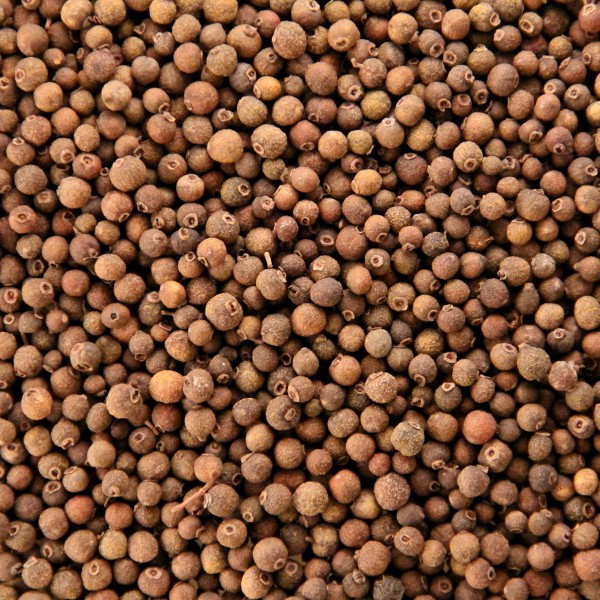
\includegraphics[width=0.3\linewidth]{imgs/spices/allspice-1.jpg}}
% 	\hfill
% 	\subfloat[\centering anise]{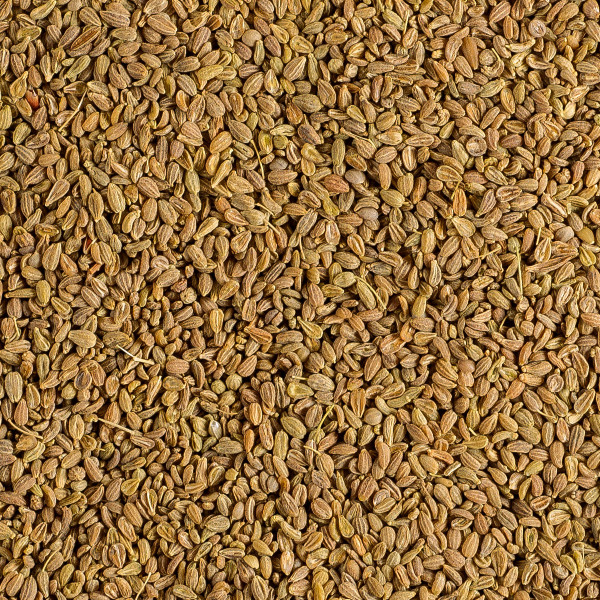
\includegraphics[width=0.3\linewidth]{imgs/spices/anise-1.jpg}}
% 	\hfill
% 	\subfloat[\centering asafoetida*]{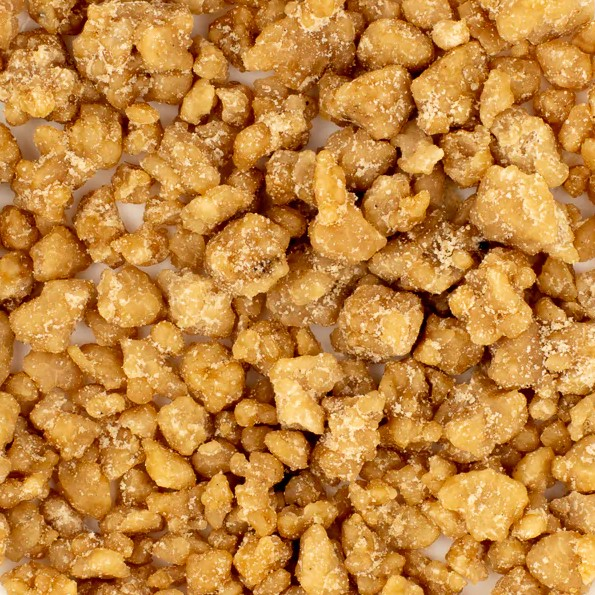
\includegraphics[width=0.3\linewidth]{imgs/spices/asafoetida-1.jpg}}
% 	\hfill
% 	\subfloat[\centering caraway]{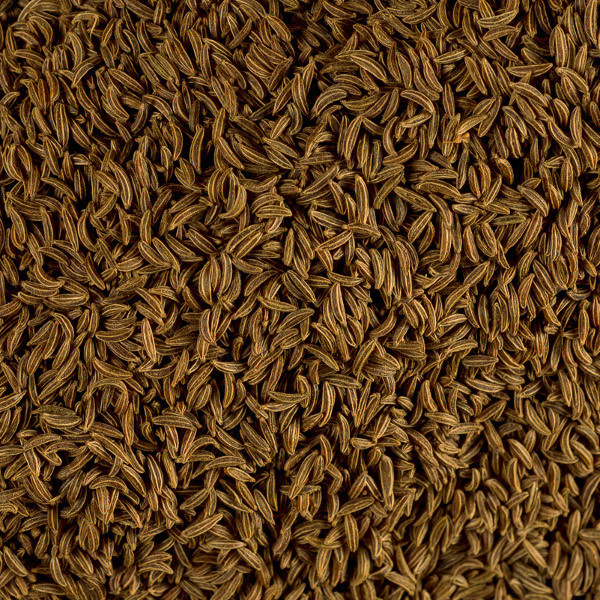
\includegraphics[width=0.3\linewidth]{imgs/spices/caraway-1.jpg}}
% 	\hfill
% 	\subfloat[\centering cardamom]{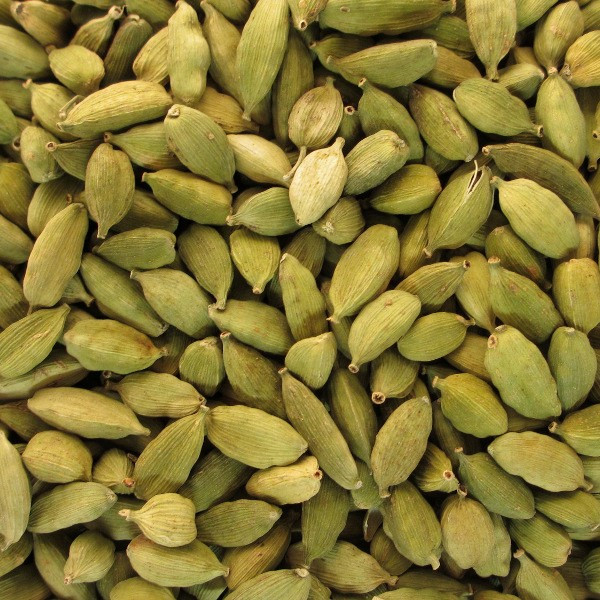
\includegraphics[width=0.3\linewidth]{imgs/spices/cardamom-1.jpg}}
% 	\hfill
% 	\subfloat[\centering cassia]{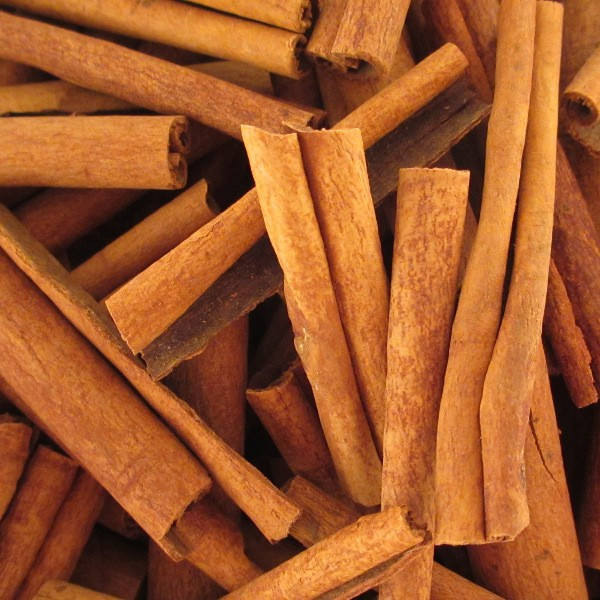
\includegraphics[width=0.3\linewidth]{imgs/spices/cassia-1.jpg}}
% 	\hfill
% 	\subfloat[\centering chile]{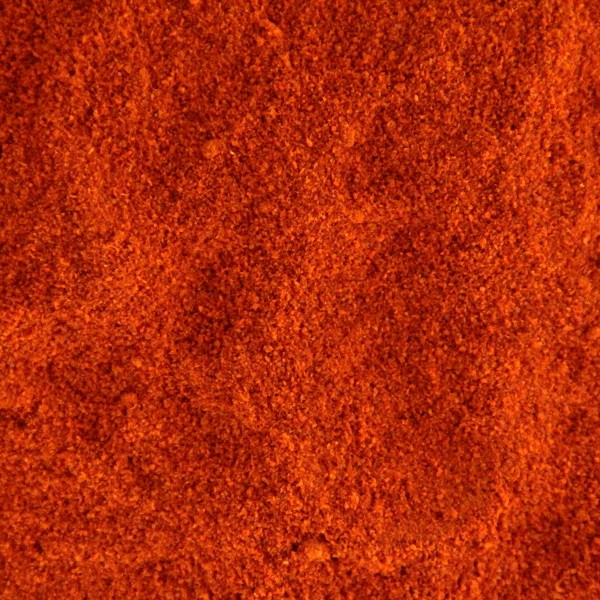
\includegraphics[width=0.3\linewidth]{imgs/spices/chile-1.jpg}}
% 	\hfill
% 	\subfloat[\centering cinnamon]{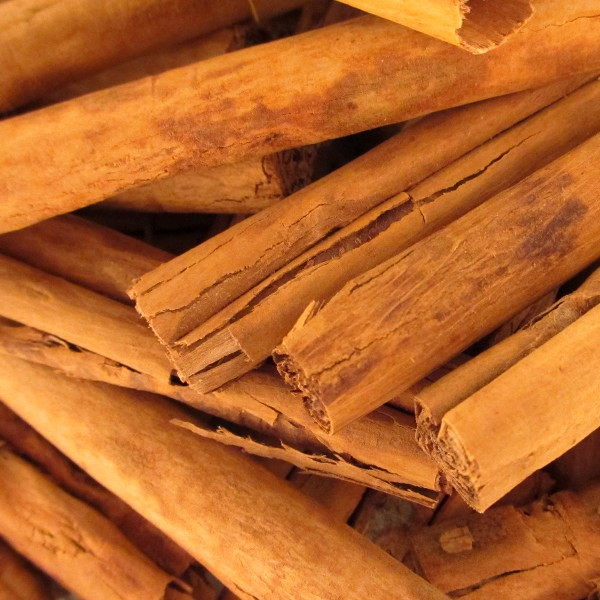
\includegraphics[width=0.3\linewidth]{imgs/spices/cinnamon-1.jpg}}
% 	\hfill
% 	\subfloat[\centering cloves]{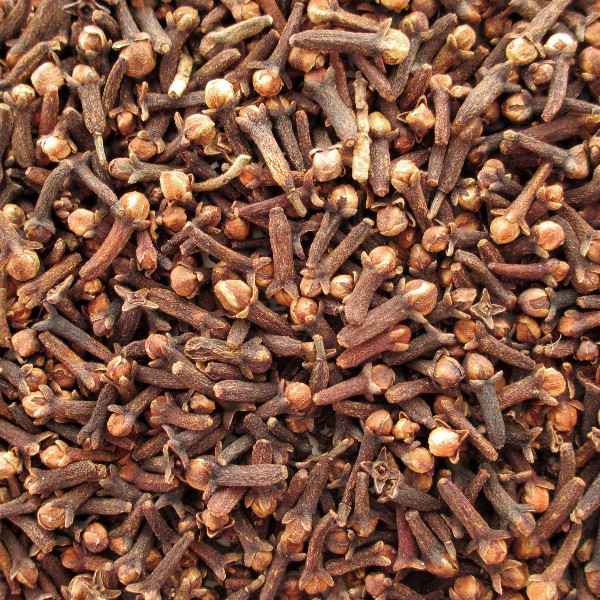
\includegraphics[width=0.3\linewidth]{imgs/spices/cloves-2.jpg}}
% 	\hfill
% 	\subfloat[\centering coriander]{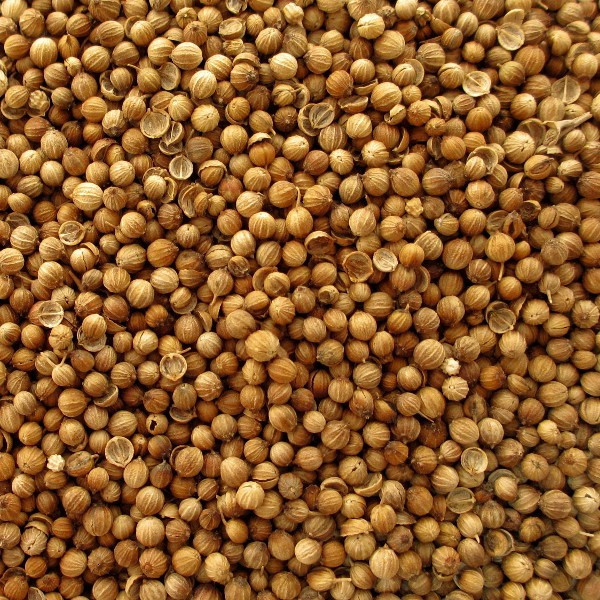
\includegraphics[width=0.3\linewidth]{imgs/spices/coriander-1.jpg}}
% 	\hfill
% 	\subfloat[\centering cumin]{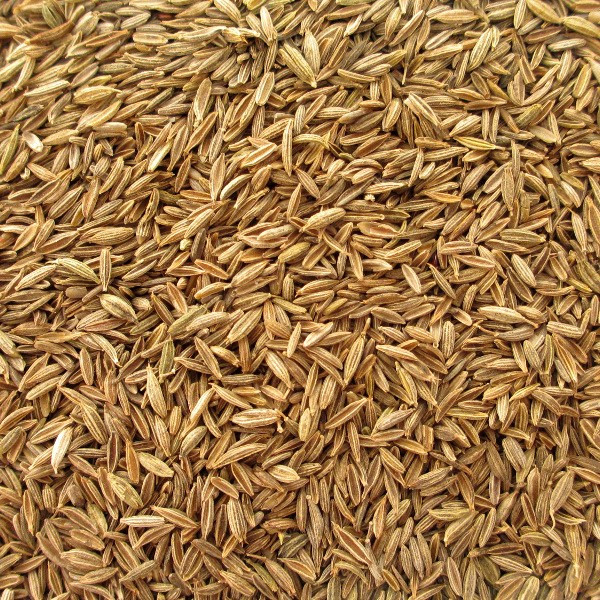
\includegraphics[width=0.3\linewidth]{imgs/spices/cumin-1.jpg}}
% 	\hfill
% 	\subfloat[\centering dill]{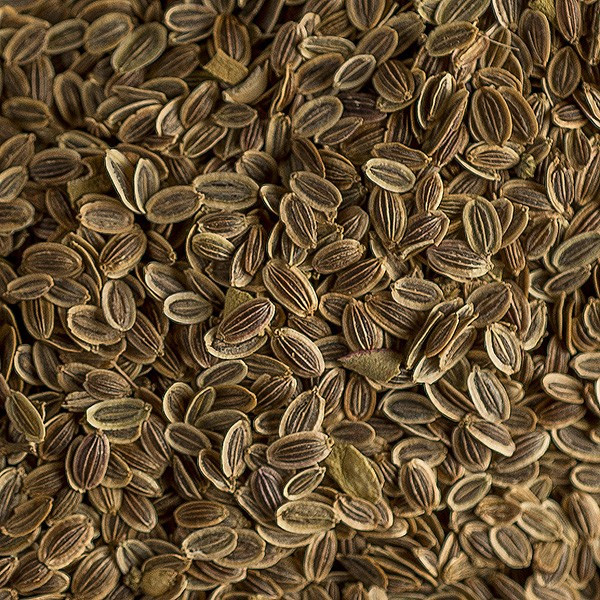
\includegraphics[width=0.3\linewidth]{imgs/spices/dill-1.jpg}}
% 	\caption[Photographs of the spices in this dissertation (I)]{Photographs of the spices in this dissertation (I). Credit: Aromatiques; *Glorian.}
% 	\label{fig:spice_imgs1}
% \end{figure}

% \begin{figure}[!ht]
% 	\centering
% 	\subfloat[\centering fennel]{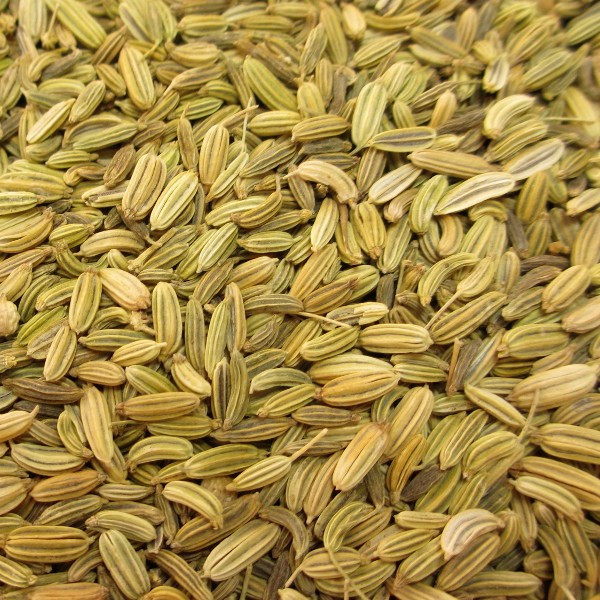
\includegraphics[width=0.3\linewidth]{imgs/spices/fennel-1.jpg}}
% 	\hfill
% 	\subfloat[\centering fenugreek]{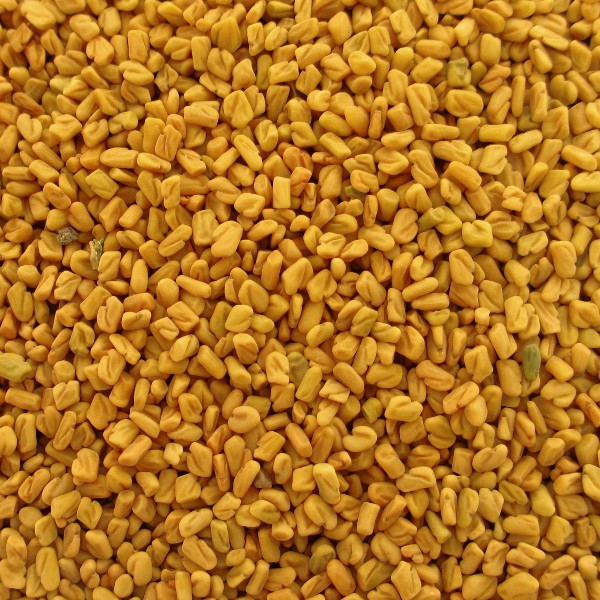
\includegraphics[width=0.3\linewidth]{imgs/spices/fenugreek-1.jpg}}
% 	\hfill
% 	\subfloat[\centering ginger]{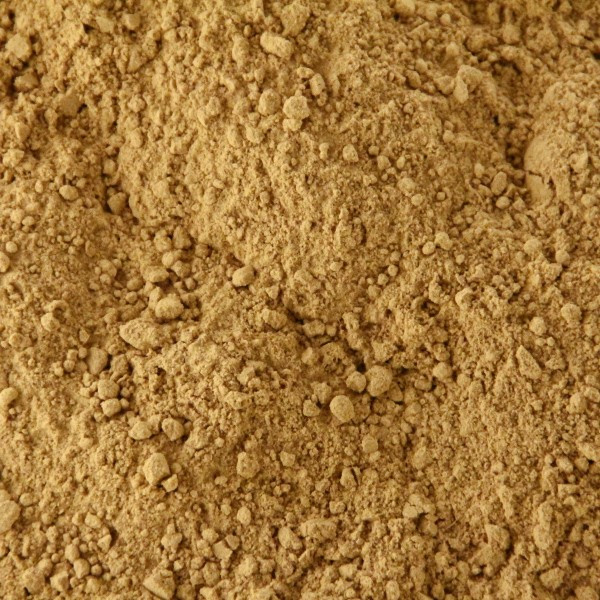
\includegraphics[width=0.3\linewidth]{imgs/spices/ginger-2.jpg}}
% 	\hfill
% 	\subfloat[\centering long pepper]{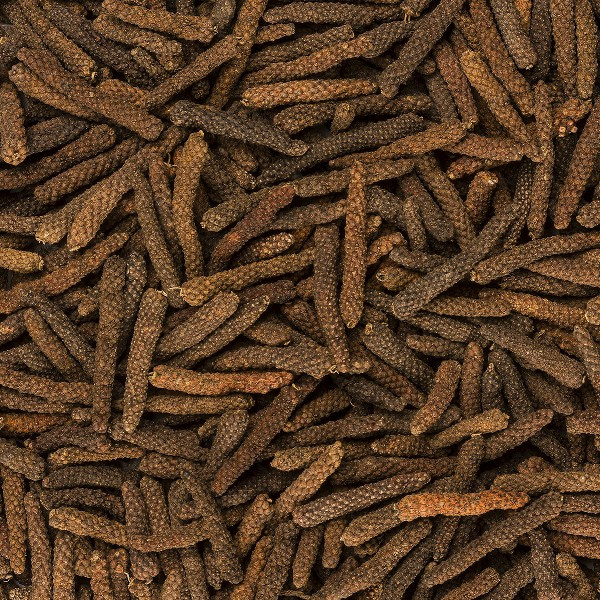
\includegraphics[width=0.3\linewidth]{imgs/spices/pepper-long-2.jpg}}
% 	\hfill
% 	\subfloat[\centering mace]{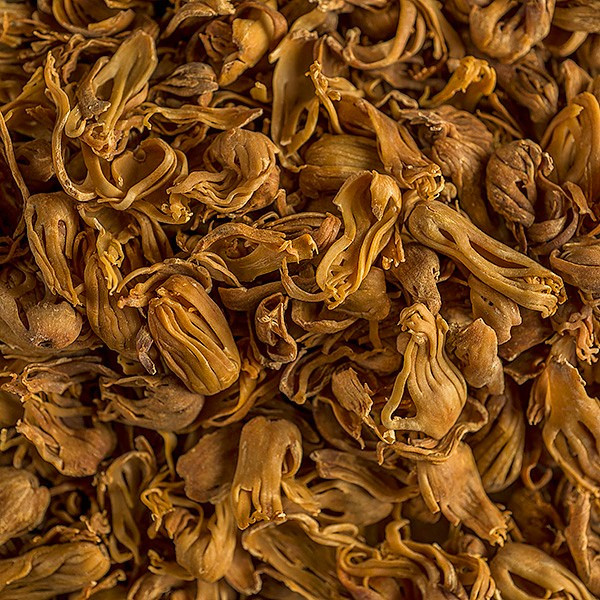
\includegraphics[width=0.3\linewidth]{imgs/spices/mace-2.jpg}}
% 	\hfill
% 	\subfloat[\centering nutmeg]{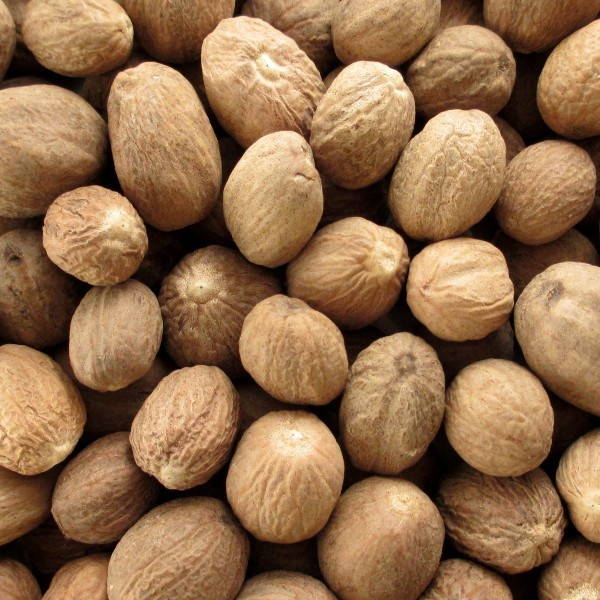
\includegraphics[width=0.3\linewidth]{imgs/spices/nutmeg-2.jpg}}
% 	\hfill
% 	\subfloat[\centering pepper]{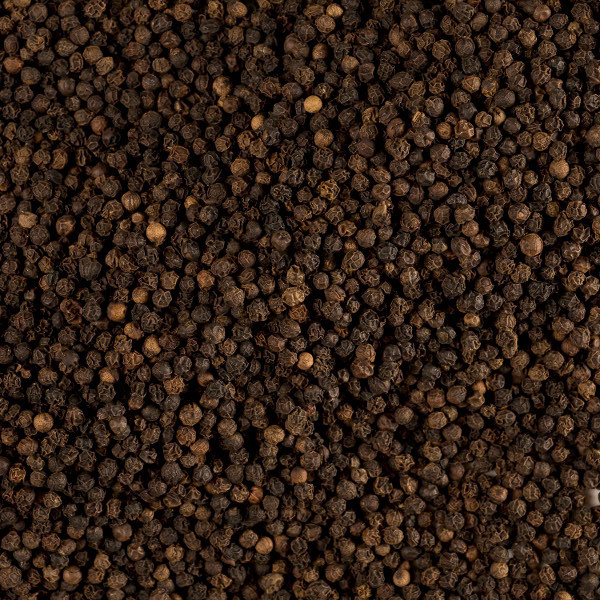
\includegraphics[width=0.3\linewidth]{imgs/spices/pepper-black-1.jpg}}
% 	\hfill
% 	\subfloat[\centering saffron]{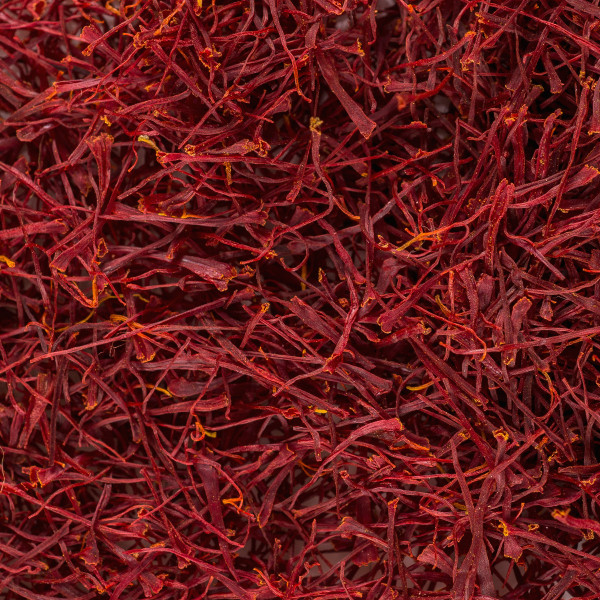
\includegraphics[width=0.3\linewidth]{imgs/spices/saffron-1.jpg}}
% 	\hfill
% 	\subfloat[\centering Sichuan pepper]{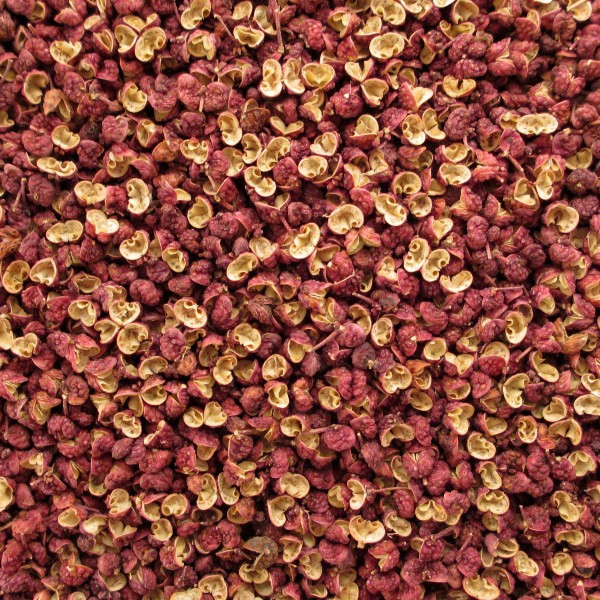
\includegraphics[width=0.3\linewidth]{imgs/spices/sichuan_pepper-2.jpg}}
% 	\hfill
% 	\subfloat[\centering star anise]{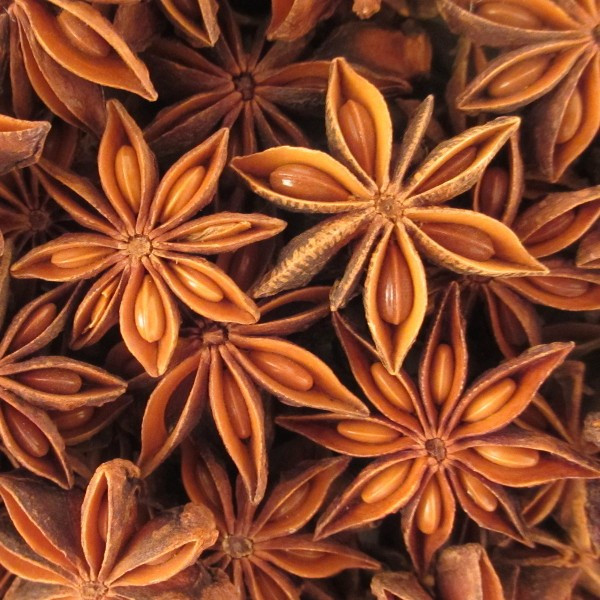
\includegraphics[width=0.3\linewidth]{imgs/spices/star_anise-1.jpg}}
% 	\hfill
% 	\subfloat[\centering turmeric]{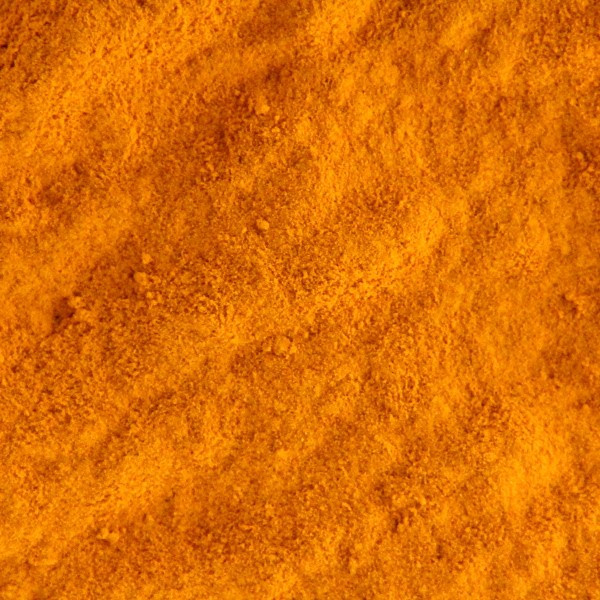
\includegraphics[width=0.3\linewidth]{imgs/spices/turmeric-3.jpg}}
% 	\hfill
% 	\subfloat[\centering vanilla]{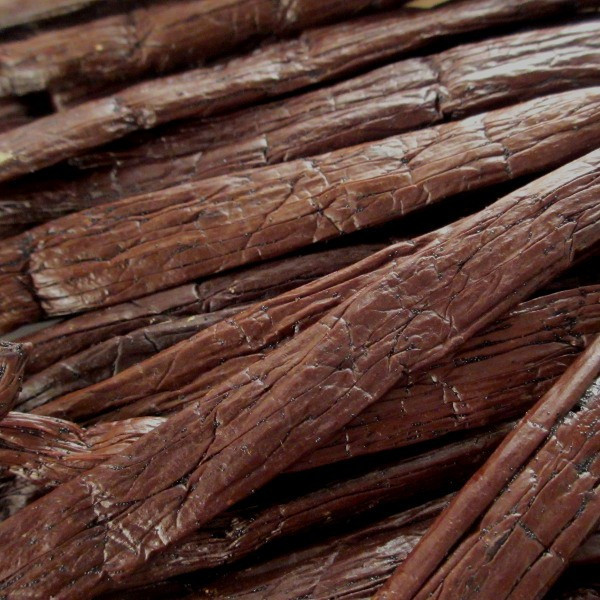
\includegraphics[width=0.3\linewidth]{imgs/spices/vanilla-1.jpg}}
% 	\caption[Photographs of the spices in this dissertation (II)]{Photographs of the spices in this dissertation (II). Credit: Aromatiques.}
% 	\label{fig:spice_imgs2}
% \end{figure}

% \clearpage % % Full page illustration
% \begin{figure}[!hbtp]
%     \centering
%     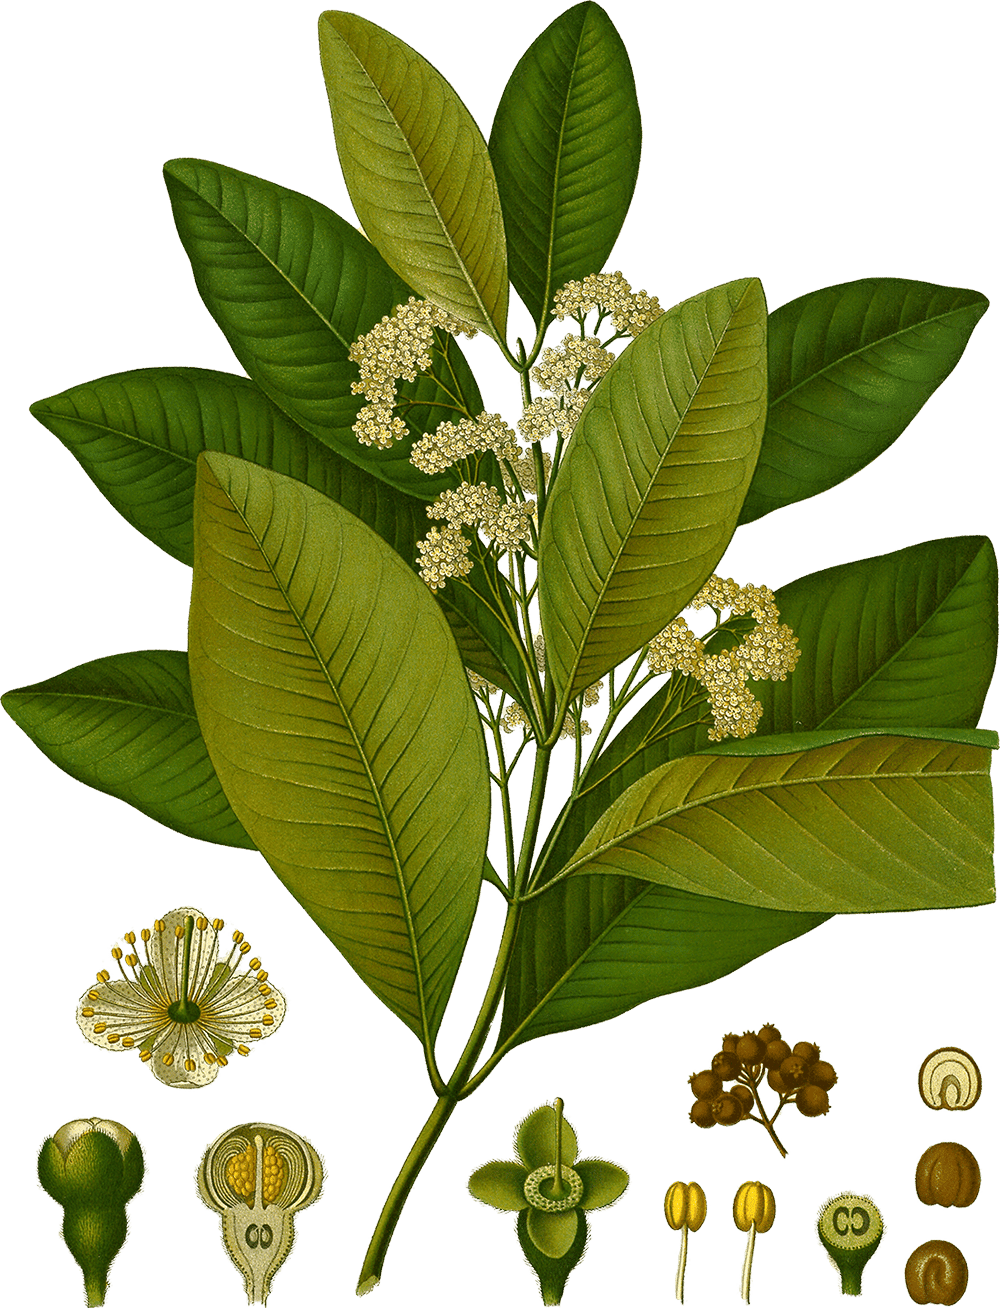
\includegraphics[width=\textwidth]{imgs/kohler/allspice_kohler_min.png}
%     \caption{\taxonn{Pimenta dioica}{(L.) Merr.} (syn. \taxonn{P. officinalis}{ Lindl.}), the allspice tree in Köhler's Medicinal Plants \pvolcite[]{2}[174]{kohler_kohlers_1887}.}
%     \label{fig:kohler_allspice}
% \end{figure}


% \begin{wrapfigure}{O}{0.5\textwidth}
%   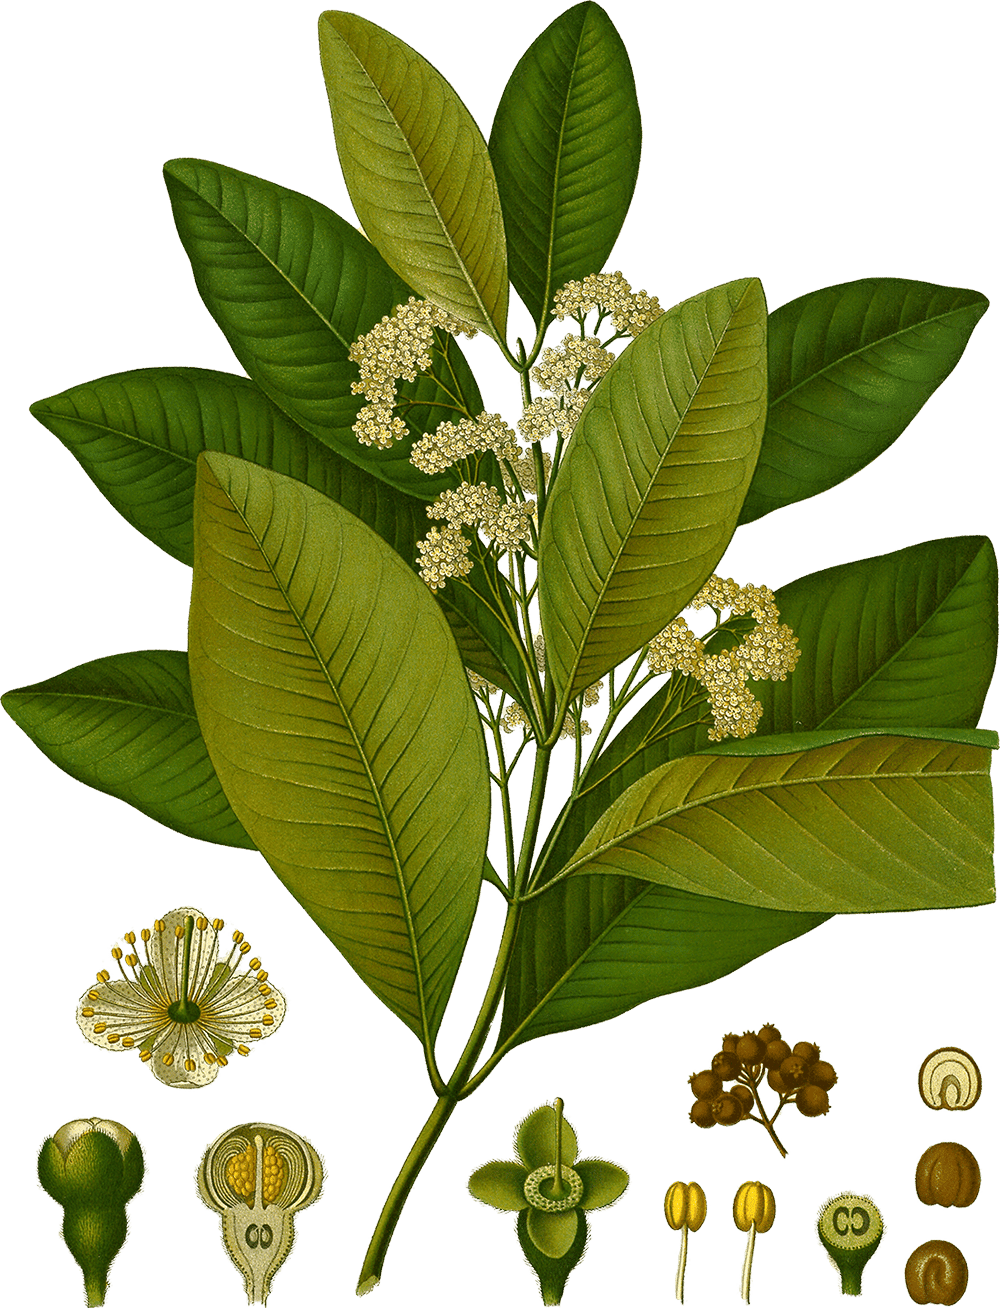
\includegraphics[width=0.5\textwidth]{imgs/kohler/allspice_kohler_min.png}
%   \caption{\textit{Pimenta dioica} {\small(L.) Merr.} syn. \textit{P. officinalis} {\small Lindl.} the allspice tree in Köhler's Medicinal Plants \pvolcite[]{2}[174]{kohler_kohlers_1887}.}
% \end{wrapfigure}


% \begin{wrapfigure}{o}{0.5\textwidth}
%     \includegraphics[width=0.5\textwidth]{imgs/spices/allspice.jpg}
%   \caption{Allspice berries}
% \end{wrapfigure}

\section{Allspice}
\label{sec:allspice}

\begin{spice}\label{spice:allspice}
\textsc{Allspice} \hfill \href{https://powo.science.kew.org/taxon/196799-2}{POWO} \\
\textbf{English:} \textit{allspice}; \textit{pimento; Jamaica pepper}. 
\textbf{Arabic:} {\arabicfont{فلفل إفرنجي}} \textit{fulful ifranjī} [Frankish pepper]. 
\textbf{Chinese:} {\tc{多香果}} \textit{duōxiāngguǒ} [many-spice-fruit]. 
\textbf{Hungarian:} \textit{szegfűbors} [clove-pepper]; \textit{jamaicaibors} [Jamaican-pepper]; \textit{amomummag} [amomum-seed].  \\
\noindent{\color{black}\rule[0.5ex]{\linewidth}{.5pt}}
\begin{tabular}{@{}p{0.25\linewidth}@{}p{0.75\linewidth}@{}}
Plant species: & \taxonn{Pimenta dioica}{(L.) Merr.} (syn. \taxonn{Pimenta officinalis}{Lindl.}) \\
Family: & \textit{Myrtaceae} \\
part used: & unripe fruit; leaf \\
Region of origin: & S. Mexico to C. America; Caribbean \\
Cultivated in: & Jamaica; Mexico; Honduras \\
Color: & dark brown \\
\end{tabular}
\end{spice}

\begin{figure}[!ht]
	\vspace{-4ex}
	\centering
	\subfloat[\centering berries]{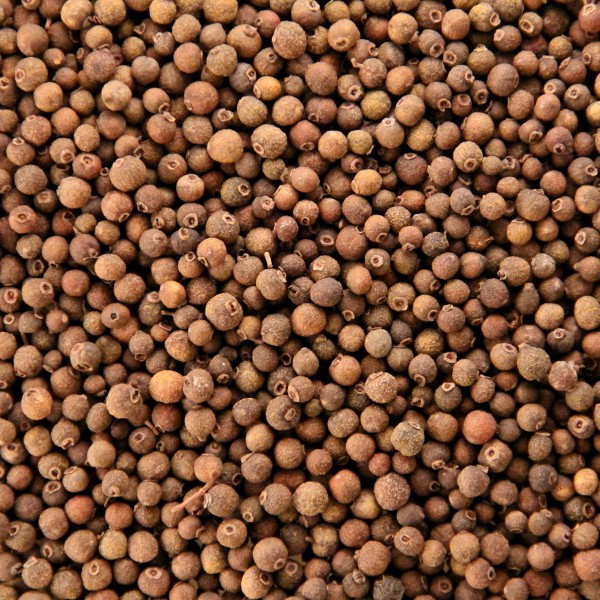
\includegraphics[width=0.3\linewidth]{imgs/spices/allspice-1.jpg}}
	\hfill
	\subfloat[\centering powder]{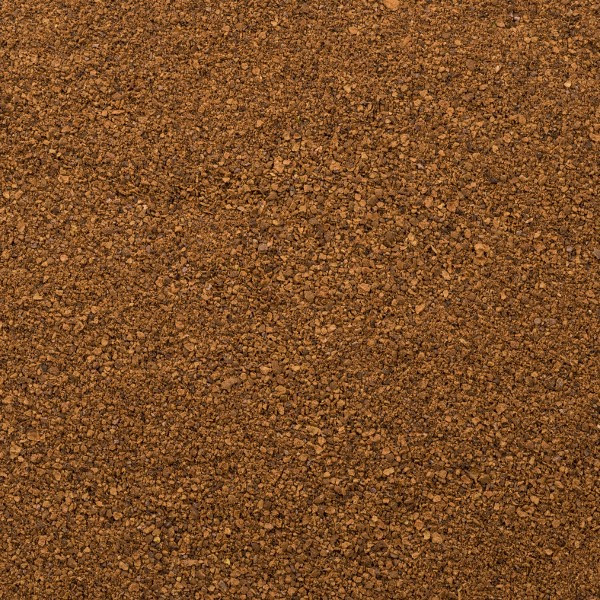
\includegraphics[width=0.3\linewidth]{imgs/spices/allspice-2.jpg}}
	\hfill
	\subfloat[\centering leaves]{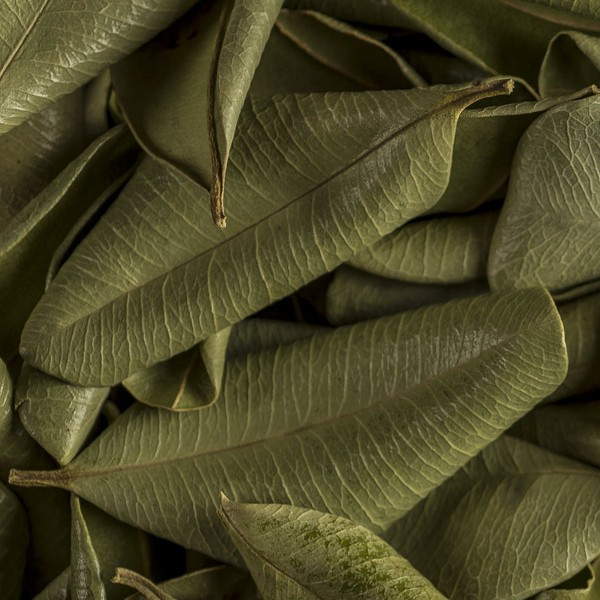
\includegraphics[width=0.3\linewidth]{imgs/spices/allspice-3.jpg}}
	\caption{Allspice berries, powder, and leaves from \textit{Pimenta dioica}.}
	\label{fig:allspice_imgs}
\end{figure}

\begin{note}
	Introducing the \textit{Spice profile box}. As it can be seen above in \textit{Spice profile} \ref{spice:allspice} presenting allspice, this business-card-like environment gives a quick reference of the spice under scrutiny in a concise way. This is intended to be a convenience for the reader to return and glance back at brief, factual information about a particular item whenever necessary. The box also contains a clickable link to the related plant species in a botanical database, \gls{POWO}, where more information can be found, such as the plants' biodiversity, distribution, botanical synonyms, as well as images of specimens.
\end{note}

%DESCRIPTION
Allspice, also known as pimento and Jamaica pepper, refers to the dried unripe fruits of a tropical evergreen tree growing in the Caribbean: the \textit{Pimenta dioica}. The dried berries are dark brown, hard to the touch, and 4--6 mm in diameter (thus larger than black pepper). Their signature crown is by a small ring of the calyx \autocite[210]{van_wyk_culinary_2014}. It is one of the few spices that do not come from the East; chili, vanilla, and allspice are the traditional three when one is listing spice products native to the Americas (disregarding cacao which is not considered a spice today). It is also the only spice that is exclusively cultivated on the western hemisphere \autocite[21]{duke_crc_2002}. The term \textit{allspice} is a coinage playing on the notion that the flavors and aroma of allspice is similar to that of clove, cinnamon, nutmeg, and black pepper \autocite[717]{mabberley_mabberleys_2017}---the most popular spices in Europe at the time when Europeans got in contact with this New World spice. People who only saw ground allspice but not whole, often tend to think that is in fact a spice mixture, after its name and rich flavor profile. Usually ground to powder, allspice is one of the key ingredients of Caribbean cuisine, especially jerk style dry-rub meat preparation. It is also used in European sausage making, pickling, baking, and flavoring liqueurs, it an overall ``handy spice''.\footnote{The Icelandic name is \textit{allrahanda}, literally `of all hands', meaning `for various purposes'; showing its multifaceted uses.} It also found its way into some Middle Eastern spice blends.


\begin{note}
\label{note:pimento}
Allspice is sometimes called pimento, which is also the name of a cultivar of \textit{Capsicum annuum}, famous from the Southern United States appetizer pimento-cheese. It is therefore important not to confuse allspice with the heart-shaped mild cherry peppers that North Americans also call pimiento or pimento. 
\end{note}

\subsection{The Botany, Origin, and  Cultivation of Allspice}

%PLANT
The allspice tree is a small mid-canopy tree or shrub with smooth, bay-like leaves and tiny white flowers. The berries turn dark purple if left to ripe, and the leaves and the bark are also aromatic \autocite[279]{riffle_tropical_1998}. Belonging to the myrtle family (\textit{Myrtaceae}), allspice is related to other aromatic trees, such as clove, eucalyptus, and the bay rum tree. Its binomial name is made up of \textit{pimenta}, the Portuguese (or corrupted Spanish) equivalent of `pepper', and \textit{dioica} `of two houses' (Greek \textit{di-} from \textit{dyo} `two' and \textit{oikos} `house'), indicating that the male and female flowers are found on different plants \pvolcite[]{2}[166]{peter_handbook_2012}.

%ORIGIN
Allspice is indigenous to the regions ranging from Southern Mexico to Central America and the Greater Antilles of the Caribbean, especially Jamaica \autocite[146]{czarra_spices_2009}. Where naturalized, it spreads by birds carrying the seeds. Allspice has been since introduced to a few neighboring places, such as Colombia, Venezuela, and Florida \autocite[][146]{powo_pimenta_2022}. In 1885 it was introduced from Jamaica to Hawaii and Kauai, 
% where it is designated as one of the most invasive horticultural plants of Hawaii \autocite{gisd_pimenta_2022}, 
and it even reached Tonga.

%CULTIVATION
Allspice is cultivated as a crop in a few countries, notably in Jamaica, Mexico, and to a lesser extent in Honduras and Grenada. The primary producer and the source of the highest quality being Jamaica. Saplings are grown from seeds, then soon transplanted when still small. The trees need well-drained soil and humid conditions \autocite[210]{van_wyk_culinary_2014}. It is one of the only spices that no one managed to grow in the East, transplantation efforts were quickly abandoned, and its commercial cultivation is confined to the Americas \autocite[21]{duke_crc_2002}. 
%HARVEST
Harvesting happens similarly to how black pepper is harvested; the still green, unripe fruits are picked by hand, and then dried under the sun.

%CHEMISTRY
The flavor of allspice mainly comes from the component eugenol, which is dominant both in the fruit and the leaves, but other compounds also add to the complexity of its aroma. Eugenol---also called clove oil, for it constitutes 80-90\% of the essential oil from clove buds \autocite[166]{barnes_herbal_2007}---is widely used as a flavoring agent by the food industry and in pharmacology, and is also found in cinnamon, nutmeg, and bay leaves. It has antiseptic, antibacterial, anesthetic, and analgesic properties \autocite{ulanowska_biological_2021}. The leaves of a related plant called the West Indian Bay Tree (\textit{Pimenta racemosa}) is used to produce bay rum, a popular essential oil used by the perfume industry for its spicy notes. 
% \todo{Contrary to popular belief, none of the above seems to be an ingredient in Old Spice\footnote{\url{https://www.fragrantica.com/perfume/Shulton-Company/Old-Spice-Original-14746.html}}}


% %USES
% \subsection{Culinary and Medicinal Uses}


% green 2006

% www.foodreference.com/html/fallspice.html
% The fruit and leaf oil are also used in men's toiletries - any time you see the word 'spice' in the name, such as in 'Old Spice' you can be sure that the fragrance comes at least in part from allspice oil. ??? no proof
% Pimento (Allspice) wood is used in Jamaica to cooked 'jerked' meats.

% Wyk:
% Allspice has become popular in some Western and East European countries, initially as a spice to replace cardamom. It is used to flavor a wide range of dishes, including meat stews, sausages, salted beef, pork, meat pastries, pickles, sauces and stuffings. Allspice is an essential ingredient of Caribbean cuisine (e.g.,jerk seasoning). It is used in Scandinavian smorgasbord, as well as fish, cheese and vegetable dishes. Mexicans use it in moles. Allspice is popular in Great Britain, where it is used in stews, sauces, confectionery, puddings and the traditional Christmas cake. Jamaican pimento dram and French liqueurs such as Benedictine and chartreuse are flavored with allspice.2 The spice, fruit oil or oleoresin extracts are commonly used in food processing, especially to flavor charcuterie items such as sausages, ham, salami and canned meats, as well as curry powders, condiments, relishes, ketchup, pickling spices and gravy mixtures. Leaf oil is used in ice creams, puddings, confectionery and liqueurs. 

% Czarra 146:
% Allspice is primarily used in the food industry in pickles, sausages, ketchup and canning meat. It can be also used as a spiced tea mix, in soups and curries and as a pickling spice.

% The fresh leaves of the allspice tree are used similarly to bay leaves in cooking, but they cannot be stored dry as opposed to the bay leaf; they lose their aroma.

%Where the tree is native, the wood is used to smoke meat.

% Duke 245
% Other Uses (Allspice) — Allspice of commerce is the dried unripe fruit, used as a condiment; in baked goods, chutney, ice cream, ketchup, mixed spices, pickles, sauces, soups; and in flavoring sausages and curing meats. Allspice powder consists of whole ground dried fruit. It’s called “allspice” because it supposedly embraces the aromas of cinnamon, cloves, and nutmeg. To make an allspice substitute, merely combine one part nutmeg, two parts cinnamon, and two parts clove (RIN). Mexican Indians used allspice to flavor chocolate. I use it to flavor eggnog. Allspice is an essential ingredient of the rubs and marinades used in seasoning Jamaican jerked foods, which are also flavored by the smoke of pimento wood fires (FAC). In Jamaica, a local drink called “pimento dram” is made of ripe fruits and rum. It is regarded as a panacea. Allspice is used in such liqueurs as Benedictine and Chartreuse. A volatile oil, extracted from the spice and leaves, is used to flavor essences and perfumes and as a source of eugenol and vanillin. The oil is also used in flavoring beverages, candies, chewing gums, liqueurs, meats and sauces, and in Asian perfumery and shaving lotions. Bahamians make a pleasing tea from the leaves. Costa Ricans use the leaves as a spice. Many ethnic groups use the leaves in tea. Saplings are used as walking sticks and umbrella handles (DAD, FAD).

% Wiki:
% Allspice is also one of the mainly used spices in Polish cuisine (used in most dishes, soups and stews) and is commonly known under the name English herb (Polish: ziele angielskie). 
% At the time allspice was encountered by Christopher Columbus during his second voyage to the New World, it was found only on the island of Jamaica, where the plant was readily spread by birds. Allspice was introduced into European and Mediterranean cuisines in the 16th century. To protect the pimenta trade, Jamaican growers guarded against export of the plant. Many attempts at growing the pimenta from seeds were reported, but all failed. Eventually, passage through the avian digestive tract, whether due to the acidity or the elevated temperature, was found to be essential for germinating the seeds,[7] and successful germination elsewhere was enabled. Today, pimenta grows in Tonga and Hawaii, where it has become naturalized on Kauaʻi and Maui.[8] It continued to be grown primarily in Jamaica, though a few other Central American countries produced allspice in comparatively small quantities.[9]

% Duke 21?

% the allspice fruits were used to preserve meats on long voyages. These preservative activities are due to some of the aromatic and antiseptic compounds which abound in allspice (anethole, caryophyllene, eugenol, linalool, pinene, and terpinene).

\subsection{The History of Allspice}

% https://journals.openedition.org/ethnoecologie/6261

There is not much we know about allspice before the arrival of the Europeans, except that the Aztecs used it to spice up their chocolate drink \autocites[27]{farrell_spices_1985}, although \textcite[145, 177]{dalby_dangerous_2000} doubts this was the case that early on. According to \textcite[21]{duke_crc_2002}, the Maya used allspice for embalming. We know that it reached Europe as a consequence of Christopher Columbus's voyages. Spanish colonizers must have encountered allspice in the West Indies sometime after Columbus and his crew explored the islands of Hispaniola, Cuba, and Jamaica, and the year 1494 is reported \autocite[12]{opara_culinary_2021}. Columbus himself did not find it. In fact, he did not recognize any spice he was so keen on finding---pepper, cloves, nutmeg, cinnamon---but kept himself and his patrons in the delusion that he will. In his first letter to Ferdinand and Isabella he writes: ``On this island there are many spices and great mines of gold and other metals. [...] I believe that I have found rhubarb and cinnamon.'' \autocite[10-18]{columbus_spanish_1893} ---in reality, he had none.\footnote{Columbus's first letter of his first voyage, sent on March 4, 1493 from Lisbon to the Spanish court (and its translation) is also available online at King's College London. Transcription: \url{http://www.ems.kcl.ac.uk/content/etext/e021.html}, translation: \url{http://www.ems.kcl.ac.uk/content/etext/e022.html}}

He was adamant that the islands he \textit{discovered} were full of spices and brought up excuse after excuse (out of season, etc.) after every voyage he returned with no spice \autocite[149]{dalby_dangerous_2000}. He also believed that he was in India or Cathay, on one of the outlying islands. Between apologies, Columbus also promised more gold, silver, cotton, mastic, and slaves. As \textcite[150]{dalby_dangerous_2000} reports, what he recorded in his private journal is a bit more honest and realistic version of events: ``I think that many trees and plants grow here which will be highly valued in Spain for dyes and medicinal spices. But I am sorry to say that I do not recognize them.'' Columbus repeatedly regrets his ignorance in botany in his journal \autocite[see also][57]{columbus_journal_2010}.

Interestingly, authors love to claim that Columbus brought back allspice (together with vanilla and chili): ``He returned with allspice from the West Indies, chilies from Mexico and vanilla from Central America.'' \autocite[17]{craze_spice_1997}, and ``Columbus brought it back to Europe thinking it was pepper.'' \autocite[146]{czarra_spices_2009}, or ``Though he did not find the Spice Islands, Columbus brought allspice, vanilla and red peppers from the West Indies back to his Spanish supporters.'' \autocite[1]{parthasarathy_chemistry_2008}. This is not true, he most likely never even saw allspice, but it was reported him that it is there and can be cultivated, along with cinnamon, and mulberry for silk production \autocites[151]{colon_life_1959}. Columbus returned from his first voyage of 1492--93 with some gold nuggets and jewelry, pearls, a hammock, tobacco, the turkey, and a few poor captured Taínos, but no spices were presented to the Spanish monarchs Ferdinand and Isabella. He did bring back pineapple and cassava \autocite[11]{turner_spice_2004}. 

Diego Álvarez Chanca, the court appointed physician who accompanied Columbus on his second expedition in 1493 is often credited with bringing home both chili, and allspice \autocites[]{mccormick_history_nodate}, but in his 1494 letter describing the flora and fauna, he only mentions \textit{agi}, also \textit{axi}---modern Spanish \textit{ají} from Taíno---\autocite[see][34]{corominas_breve_1987}, and that the natives use it to season their food, with what we now know as \textit{Capsicum annuum}: the chili pepper \autocite[311]{chanca_american_2003}.

In the following century the Spanish tried to turn Mexico into a spice plantation by transplanting eastern spices, an effort that mostly failed. Only after this did the colonizers start to pay proper attention to native spices \autocite[6]{machuca_past_2020}. 

Francisco Hernández de Toledo, King Philip II's court physician and naturalist spent 7 years in New Spain between 1571--1577, studying its species and conducting interviews with the natives. He was the first to formally describe allspice. He called it \textit{Pipere Tavasci} `Tabasco pepper' (today \textit{Pimienta de Tabasco}, after the region of Tabasco, famous today for a brand of hot sauce. Hernández also recorded the Nahuatl name of allspice: \textit{xocoxochitl} `sour flower'.\footcite[cf.][xococ; xochitl]{ond} Hernández likens the flowers to pomegranates, and and the aroma to that of orange blossoms, describing it to be very pleasant and attractive, with a sharp taste of the fruit. \autocite[2]{hernandez_cuatro_1615}. In \textcite{machuca_past_2020}'s translation:

\begin{quote}
    ``Xocoxochitl meaning sour flower, is a large tree, with leaves like those of the oranges, red flowers like a pomegranate, but with an aroma like the orange blossom, and in such a smooth and pleasant way, that even the leaves of the tree add to its attraction: the fruit is round, and hangs in clusters, which at first appear green, and then beige, and finally towards black: it is sharp and scathing to taste, and good-smelling'' 
\end{quote}

According to \textcite{machuca_past_2020}, although allspice was known by the Spanish from early on ``there are few historical records of its production and trade'', and only in the \nth{18} century started they to consider American products to have economic potential.
 
Allspice berries are around 30\% larger then peppercorns, and since their color and shape resembles black pepper, and it gave a spicy taste to food, it is no wonder that the Spanish called them \textit{pimiento} `pepper'. The Portuguese version is \textit{pimento}, and later the botanical name \textit{Pimenta} was given to the genus of plants related to allspice \autocite[26]{farrell_spices_1985}. I disagree with the often repeated trope that the Spanish explorers mistook allspice berries for pepper and called them \textit{pimiento} ``by mistake''\footcite[allspice \link{https://www.britannica.com/plant/allspice}]{britannica_spice_2022}, these people knew exactly what they were looking for, and that what they have found is not the mighty black pepper; but for them it was a kind of pepper. The crew showed samples of pepper and cinnamon to presumably confused Native Americans hoping for directions, and as Columbus wrote in his journal on the \nth{4} of November, 1492, they indicated by sign language that there is a lot of it around \autocites[21]{duke_crc_2002}[67]{columbus_journal_2010}. The Europeans, however, soon recognized the value of allspice, even if it was not the expensive black pepper, but still more pungent and exotic than some cheap Old World substitutes, the juniper and myrtle berries (which are very similar to allspice in appearance and usage)  \autocite[150]{dalby_dangerous_2000}.

In short, allspice was introduced to Europe by the Spaniards in the \nth{16} century, its import was first recorded in 1601, according to \textcite{britannica_allspice_nodate} and \textcite[26]{farrell_spices_1985}. After 1655, when Jamaica became a British colony for nearly three centuries, the Brits developed a taste for allspice and started to use it to season meat dishes, sauces, and pickles \autocite[74]{green_field_2006}. They were also responsible for its spread to some extent which is illustrated by the names of allspice in some languages, e.g.,Polish \textit{ziele angielskie} `English herb'.

% Allspice was first exported to Europe in 1601 as a substitute for cardamom. ?? Farrell 26

% https://www.mexconnect.com/articles/3799-fragrant-flavorful-allspice-an-essential-mexican-seasoning/

% peter 2 167
% The berries reached London in 1601 as described by Clusius in his Liber Exoticorum and the plants were first cultivated in England in a hot house in 1732 (Weiss, 2002). Before World War II, allspice was more widely used than today; however, during the war many trees were cut down and there was a shortage of the spice. Although cultivation was taken up after the war, production never fully recovered.


\subsection{The Names of Allspice}

Allspice is a fascinating case, because it gives us examples for a plethora of names that showcase us many of the motivations, mechanisms, and solutions people choose when naming spices. As I mentioned before, some people are puzzled if allspice is a spice blend or not. The names in some languages often just add to the confusion, for example French \textit{quatre-épices} (lit. `four spices') can have the sense `allspice', but also `a kind of spice mix' made up of four different spices.\footcite[quatre-épices \link{https://www.cnrtl.fr/definition/quatre-\%C3\%A9pices}]{tlfi}


% All these names can be explained by the characteristics, use, and journey of allspice. Let us now consider the names in English, Arabic, and Chinese.

\subsubsection{English}

\begin{etymology}\label{ety:allspice}
\textbf{English} \textit{allspice}, from \textit{all} + \textit{spice}; after the flavor profile that resembles the combined aroma of cloves, nutmeg, cinnamon, and black pepper, 1621\footnote{\textcite[s.v. allspice]{oed}}
\end{etymology}

\begin{note}
	Introducing the \textit{Etymology box}. This environment, as seen above in \textit{Etymology} \ref{ety:allspice}, offers a quick look at a words' origins and development.
\end{note}

Since its introduction to the spice cabinet, allspice has been known by many names from which currently \textit{allspice} \index{allspice|textbf} seems to be prevailing. \textit{Allspice} was formed by compounding \textit{all} and \textit{spice}, for its flavor was perceived to be a combination of four characteristic spices that the Europeans knew and sought after: black pepper, cinnamon, cloves, and nutmeg.\footcites[allspice]{oed}[]{britannica_allspice_nodate} It was first recorded in 1621: ``Ambergreese, nutmegs, and all spice.''\footcite[allspice]{oed}, and probably inspired the French \textit{toute-épice} `all-spice', attested in 1762.\footcite[toute-épice \link{https://www.cnrtl.fr/etymologie/toute-\%C3\%A9pice}]{tlfi}

Sadly, the original word for allspice was lost with the demise of the native Taíno people of the Caribbean, nevertheless we got Taíno\footnote{Taíno is a now extinct Arawakan language.} words such as barbecue, \textit{cassava}, \textit{guava}, \textit{hammock}, and \textit{tobacco} \autocite[229]{rafinesque_american_1836}. As we concluded before, it is assumed that it was the Spanish who first got in contact with the allspice berry, and that they simply called it \textit{pimienta} `pepper'.

\begin{etymology}\label{ety:pimento}
\textbf{English} \textit{pimento} `allspice; sweet pepper', ca. 1660
< partly \textbf{Portuguese} \textit{pimenta} `allspice; sweet pepper; black pepper'
< and partly \textbf{Spanish} \textit{pimiento} `hot and sweet pepper; formerly also black pepper; pepper plant of both kinds', earlier \textit{pimienta} `black pepper; peppercorn; ground pepper' \nth{13} c., 1495
< \textbf{Medieval Latin} \textit{pigmenta} `plant juice; food seasoning; condiment; spices; perfumes', plural of \textit{pigmentum}
< \textbf{Latin} \textit{pigmentum} `colour, paint; ointment; drug; spiced wine', from \textit{pingō} `to paint' + \textit{-mentum} `instrument'\footnote{\textcite[s.v. pimento]{oed}; \textcite[s.v. pimento]{oed}; \textcite[s.v. pimiento]{oed}; \textcites[415]{gomez_de_silva_elseviers_1985}[495]{corominas_breve_1987}; \textcite[s.v. pigmentum]{lewis_latin_1879}}
\end{etymology}

For a long time \textit{pimento} (and to a much lesser extent \textit{pimiento})---the words for `pepper' in Portuguese and Spanish, respectively---was commonly used in English to refer to allspice. This is still the case in Jamaican English for example, where the term \textit{allspice} is not used. In North American English however, \textit{pimento} now rather refers to a small, round variety of chili pepper (\textit{Capsicum annuum}), commonly known as cherry pepper explained in \cref{note:pimento}. 

The corruption and mix-up between the English words \textit{pimento} and \textit{pimiento} and their origins is as confusing as it gets. For the sake of a clear understanding, let us first consider the modern names for allspice in Spanish: \textit{pimienta de Jamaica}, and Portuguese: \textit{pimenta-da-jamaica}. In both cases, \textit{pim\-(i)enta}, with a final \textit{-a}, means `pepper', referring to peppercorns of the usual black and white pepper (\textit{Piper nigrum}). In Spanish and Portuguese, the words endings of \textit{-o} and \textit{-a} mark the grammatical gender, the significance of which dissipates in English. It is important to remember however, that the Spanish form \textit{pimienta} emerged first from a Latin neuter plural suffix in the \nth{13} century. Thus, perhaps a century or so later when the word \textit{pimienta} was already embedded in Spanish, speakers perceived the word as a feminine noun, and a vacuum of a masculine counterpart emerged. This allowed for a practical differentiation by gender between the peppers of the Old Word and the New World. \textcite[459]{corominas_breve_1987} explains that \textit{pimiento} derived from \textit{pimienta}, and it was first applied in the Americas for the red fruits of the chili.

\textcite[415]{gomez_de_silva_elseviers_1985} makes the most compact distinction: ``\textit{pimienta} `(black) pepper; allspice', \textit{pimiento} `(hot and sweet) pepper' ''. In contemporary Spanish, \textit{pimiento} (the masculine form) refers to the fruits and plants of the \textit{Capsicum} family, e.g.,the numerous spicy chilies and mild bell peppers of red, green, and yellow, while \textit{pimienta} (the feminine form) refers to the small round fruits of black and white pepper and its powdered forms. The distinction seems consistent, belonging to this latter group see for example \textit{pimienta dulce} `sweet pepper', and \textit{pimienta gorda} `fat pepper' both of which refers to allspice, not to be confused with \textit{pimiento dulce}, which refers to sweet paprika powder.\footcite[pimiento, -a]{dle}

\textit{Pimento} in English is a partly Portuguese, partly Spanish borrowing, while \textit{pimiento} comes from Spanish. In fact, it is explained in the \gls{OED} that in the `allspice' sense of the word, \textit{pimento}, from Portuguese \textit{pimenta (da Jamaica)}, went through an alteration influenced by the Spanish word form, which is not attested in the `allspice' sense. Ergo, Spanish \textit{pimiento} maybe did not refer to allspice in Spanish at the time when the borrowing happened. And if so, \textit{pimento} is a borrowing from Portuguese \textit{pimenta} meaning `pepper' and, as \textit{pimenta da Jamaica}, `allspice', influenced by Spanish \textit{pimiento} `chili, sweet pepper', also in the sense of the pepper plants of both kinds (chili and black). Spanish \textit{pimiento} formerly had the sense of `black pepper, peppercorns, and ground pepper' (before 1495), with an earlier form \textit{pimienta} (\nth{13} century), now usually in sense ground pepper and peppercorns\footcite[pimento]{oed}. The Portuguese connection is only discussed by the \gls{OED}, other dictionaries do not mention it. A direct Spanish borrowing is also plausible if we consider that it was the Spanish who most likely brought it back first, they probably called it \textit{pimiento/-a}, and they were responsible for its subsequent diffusion in Europe. English spellings varied greatly of this this Romance word, using forms such as \textit{piemente} in the late 1600s. 

The origin of these words is the classical Latin \textit{pigmentum} `a material for coloring, a color, paint, pigment', with a transferred meaning `the juice of plants' in post-classical Latin.\footcite[pigmentum \link{http://www.perseus.tufts.edu/hopper/morph?l=pigmentum\&la=la\&can=pigmentum0\#lexicon}]{lewis_latin_1879} The word \textit{pigmentum} is made up of \textit{pingō} `to paint' and \textit{-mentum}, a suffix denoting an `instrument, medium', well recognizable from Romance languages and English (i.e.,excite\textit{ment}).
According to \textcite[459]{corominas_breve_1987}, Catalan \textit{pimienta} is attested in the \nth{13} century and it comes from the plural (\textit{pigmenta}) of Latin \textit{pigmentum} `coloring, paint', which already meant `drug, ingredient', and later, `condiment' in Medieval Latin. Derived from this, in 1495 \textit{pimiento} was applied to the plants bearing the pungent red fruits of the Americas. \textit{Pigmentum} also entered English as \textit{pigment} `paint, dye, ingredient in an ointment, drug'. According to the \gls{OED}, Medieval Latin \textit{pigmentum} also referred to spiced drinks (\nth{9} century), perfumes, and hence spice in general. Old French cognates support this, \textit{pigment} had the sense of `balm, fragrant spice' in the \nth{12} century, Anglo-Norman \textit{pigment/piment} meant `spice, spice wine'\footcite[pigment]{oed}, and Middle English \textit{pihmentum} (\nth{12} century, later \textit{piment}) had a sense of ``a spiced drink, a remedy or concoction containing spices'',\footcite[pigment]{oe} ``a sweetened, spiced wine used for refreshment and in medical recipes; a medicinal potion''.\footcite[piment]{med} \textit{Piment} in French were later applied for chili, especially the cultivar of cayenne pepper. (The \gls{OED} points to the sense `cayenne pepper' in a ``\nth{10} century French source'', which must be an error.)


Allspice is also known as \textit{Jamaica pepper}, for it mainly grows on the island and the historical reasons described above. Many languages calqued \textit{pimienta de Jamaica} from Spanish, or another transmitting language (e.g.,Italian \textit{pepe della Giamaica}). \textit{Jamaica pepper} was first recorded in 1661: ``A kind of Pepper, that tastes like Cloves, and very Aromatick (known by the name of Iamaica-Pepper)''.\footcite[Jamaica]{oed}

The name \textit{myrtle pepper} \index{pepper!myrtle} echoes the similarities of the allspice tree with European myrtle (\textit{Myrtus communis}), especially after the resemblance of their purple berries. Beyond the physical resemblance, myrtle berries are also edible, and are also dried to add to pepper mills as a spice. Furthermore, the European myrtle has aromatic leaves and wood as well, and it is used to grill and smoke meat in Southern Europe since Roman times, especially on Sardinia and Corsica; the same way the Caribbean people use allspice wood and leaves. The myrtle berry appears in Roman and Greek mythology as well \autocite[186]{van_wyk_culinary_2014}.

The name \textit{clove pepper} has ``chemical reasons'', namely that this name arises from the aroma of allspice that reminded people of clove. This is due to its eugenol content we discussed above. \textit{Szegfűbors} lit. `clove-pepper' is the most common name for allspice in Hungarian still, and it is used in sausage making.

One of the most interesting spice names we can come across in my opinion is \textit{newspice}. The term is now archaic in English, but the idea still exists in a few European languages, such as Serbian and Macedonian \cy{најгвирц} \textit{najgvirc} from German (\textit{Neugewürz}), Czech and Slovak (\textit{nové koření/korenie}), and Turkish \textit{yenibahar} and Romanian \textit{ienibahar} from Ottoman Turkish \ar{یڭیبهار} \textit{yeñibahar}; all the above literally meaning `new spice'.

The reason behind these names is that during the 17-\nth{18} centuries, allspice ``suddenly'' arrived to Central and Eastern Europe as a new (and possible marketed as a trendy) spice. This happened a century after the red hot paprika took the world by storm (by \nth{16} century it reached Hungary from the Ottoman Empire), and while the chili did not conquer northern Europe, allspice---to an extent---did. We could philosophize why the chili did not deserve the name `new spice' when it first arrived, or why the Europeans---except on the south---were reluctant to assimilate it into their cuisines. Was the pungent chili too harsh for a Northern palate to consider? Is it the sophisticated chemical complexity of allspice that made it fashionable in Victorian England? All these questions are leading us to deep waters regarding the human palate and cultural attitudes toward spices and spiciness, as well as environmental and genetic factors deciding the heat of preference explored by interesting papers such as \textcite{tornwall_why_2012,spence_why_2018}.

We know that in the beginning allspice was overlooked by Europeans, and this is possibly the reason why allspice's original name did not survive unlike the Nahuatl word \textit{chīlli}. Allspice was was later sold and used in beverages and cookery, but its rising star never came close to that of chili.
In Asia, where chilies were adopted early on and, eagerly transplanted, they transformed and revolutionized cuisine forever. It is unimaginable to think of Indian, Indonesian, or Chinese dishes without chilies today. Inversely, allspice is mostly unknown in East Asia, and the reasons behind it are just as botanical as historical: In the 16-\nth{17} century nobody knew how to grow allspice, while chili can be grown everywhere effortlessly. In addition, Europeans did not sail to Asia to sell spices, they went to take them. 

As the \nth{20} century came around, allspice---the only spice still exclusively imported from the Western hemisphere---quietly became one of the many, and its fervor faded a little. America was not new anymore, and the name \textit{new spice} as well became obsolete. An English textbook for students of Italian narrates a letter from 1680 about this \textit{Nuova Spezie} and the author's opinion on it:

\begin{quote}
``I Am much obliged to you for the Drug you sent me inclosed in your last letter, about which I cannot tell you any thing but that it is called the New Spice, and it comes as it is said, or as it is guessed, from the West-Indies, and not from the East-lndies; and it is but six months that I had knowledge of it from Count Laurence Magalotti, who showed it me under the abovesaid name of New Spice. How many different tastes are found in it by several honest folks ! that of the clove is the principal ; that of the nutmeg is the second in rank ; the cinnamon comes as it were the third in order ; next the citron ; then the smell of the musk and of the amber, and the most sweet taste of sugar. The truth is, in my opinion, that it is a pretty Drug. I am in Florence, and with for an occasion to do you service ; so command me with all freedom, and be certain that I will count it as good luck to have any power to serve you. I affectionately kiss your hands. Florence, 26th March 1680.'' \autocite[5]{baretti_introduction_1755}
\end{quote}

% \begin{quote}
% ``I Am much obliged to you for the Drug you \lgS ent me inclo\lgS ed in your la\lgS t letter, about which I cannot tell you any thing but that it is called the New Spice, and it comes as it is \lgS aid, or as it is gue\lgSS ed, from the We\lgS t-Indies, and not from the Ea\lgS t-lndies; and it is but \lgS ix months that I had knowledge of it from Count Laurence Magalotti, who \lgS howed it me under the above\lgS aid name of New Spice. How many different ta\lgS tes are found in it by \lgS everal hone\lgS t folks ! that of the clove is the principal ; that of the nutmeg is the \lgS econd in rank ; the cinnamon comes as it were the third in order ; next the citron ; then the \lgS mell of the mu\lgS k and of the amber, and the mo\lgS t \lgS weet ta\lgS te of \lgS ugar. The truth is, in my opinion, that it is a pretty Drug. I am in Florence, and with for an occa\lgS ion to do you \lgS ervice ; \lgS o command me with all freedom, and be certain that I will count it as good luck to have any power to \lgS erve you. I affectionately ki\lgS s your hands. Florence, 26th March 1680.''
% \end{quote}

And so, we have established a few categories when it comes to the names of allspice: (1) names that are made up of \textit{spice} as a headword and a modifying word, (2) names that use \textit{pepper} as a headword with a modifier, and (3) names that are taken from Portuguese and Spanish. See \cref{table:names_allspice_en} for a concise overview.

\begin{table}[!ht]
\caption{Various names for allspice in English.}
\centering
\begin{tabularx}{\textwidth}{@{}l>{\itshape \small}lL>{\small}l@{}}
\toprule
\textbf{\#} & \multicolumn{1}{l}{\textbf{Species}} & \multicolumn{1}{l}{\textbf{Name}} & \multicolumn{1}{l}{\textbf{Source}} \\
\midrule
\textbf{1}	& \textbf{Pimenta dioica}	& \textbf{allspice}	& \textbf{\textcite{van_wyk_culinary_2014}} \\
2	& Pimenta dioica	& clove pepper	& \textcite{duke_crc_2002} \\
3	& Pimenta dioica	& Jamaica pepper	& \textcite{van_wyk_culinary_2014} \\
4	& Pimenta dioica	& myrtle pepper	& \textcite{peter_handbook_2012} \\
5	& Pimenta dioica	& newspice	& \textcite{peter_handbook_2012} \\
6	& Pimenta dioica	& pepper cloves	& \textcite{james_pimento_2022} \\
7	& Pimenta dioica	& pimento	& \textcite{van_wyk_culinary_2014} \\
8	& Pimenta dioica	& pimento berry	& \textcite{oed} \\
9	& Pimenta dioica	& pimiento	& \textcite{oed} \\
\bottomrule
\end{tabularx}
\label{table:names_allspice_en}
\end{table}



\subsubsection{Arabic}

\begin{etymology}\label{ety:fulful ifranji}
\textbf{Arabic} {فلفل إفرنجي} \textit{fulful ifranjī} `allspice' [European pepper], literally `Frankish pepper', named so because it was transmitted by Europeans, 1700?\footnote{\textcite{baalbaki_-mawrid_1995}}
\end{etymology}

Arabic, similarly to English, boasts with a diverse set of names when it comes to allspice. First and foremost, it is known as \textit{filfil ifranjī} `European pepper'. \textit{Ifranjī} literally translates to `Frankish', but it became the epithet of white Europeans, similarly to the term \textit{farang}\footnote{A word of Persian origin, applied for the Franks during the crusades (from Old French \textit{franc}), and later by extension to any white merchant used from Persia to Thailand.} in Southeast Asia. The rationale behind this name is evident: it was Europeans who introduced this spice to the Middle East and North Africa in the centuries following its debut. %18-19 centuries?

Allspice's Middle Eastern history is the topic I have found the least amount of information on, considering every other spice in this chapter. As it is an ingredient that have arrived long after the classical times, it is not discussed in the literature I have consulted, and modern articles only deal with it for its pharmaceutical and health benefits, not with its journey. The challenge to find further Arabic synonyms is also increased, because both English names \textit{allspice} and \textit{pimento} are ambiguous. I have found examples of wrongly glossed entries in both Arabic, and Chinese dictionaries. Be that as it may, I have managed to collect a few other Arabic names for allspice from contemporary dictionaries, these can be seen in \cref{table:names_allspice_ar}. 

Further common vernacular names are \textit{fifil ḥulw} lit. `sweet pepper', and \textit{bahār ḥulw} lit. `sweet spice', where \textit{bahār} `spice', is a loanword from Persian. Persian \fa{بهار} \textit{bahār} means spring (the season), it was borrowed into Arabic with a sense of blossoms and foliage, alluding to the leaves and flowers of plants as the source of many spices.\footcite[121]{dozy_supplement_1881} In the `spice, seasoning, condiment' sense, the word spread regionally via Ottoman Turkish (loaned from Arabic). Similarly to the case of English, the word for spice was associated with the allspice berries, and consequently resulted in the already mentioned Turkish \textit{yenibahar} [newspice] `allspice', and \gr{μπαχάρι} \textit{bachári} `allspice'. Thus, just like English, Arabic propagates allspice names by using the words for `spice' and `pepper' with modifiers indicating qualities of taste, or who carried the spice.

\begin{table}[!ht]
\caption{Various names for allspice in Arabic.}
\centering
\begin{tabularx}{\textwidth}{@{}l>{\itshape \small}lr>{\itshape}lL>{\small}l@{}}
\toprule
\textbf{\#} & \multicolumn{1}{l}{\textbf{Species}} & \multicolumn{1}{l}{\textbf{Name}} & \multicolumn{1}{l}{\textbf{Tr.}} & \multicolumn{1}{l}{\textbf{Gloss}} & \multicolumn{1}{l}{\textbf{Source}} \\
\midrule
1	& Pimenta dioica	& بهار حلو	& bahār ḥulw	& sweet spice	& \textcite{wiktionary} \\
2	& Pimenta dioica	& فلفل البساتين	& fulful al-basātīn	& pepper of the gardens	& \textcite{almaany} \\
\textbf{3}	& \textbf{Pimenta dioica}	& \textbf{فلفل إفرنجي}	& \textbf{fulful ifranjī}	& \textbf{European pepper}	& \textbf{\textcite{baalbaki_-mawrid_1995}} \\
4	& Pimenta dioica	& فلفل تابل	& fulful tābil	& spice pepper	& \textcite{almaany} \\
5	& Pimenta dioica	& فلفل حلو	& fulful ḥulw	& sweet pepper	& \textcite{baalbaki_-mawrid_1995} \\
\bottomrule
\end{tabularx}
\label{table:names_allspice_ar}
\end{table}



\subsubsection{Chinese}

\begin{etymology}\label{ety:duoxiangguo}
\textbf{Mandarin Chinese} {多香果} \textit{duōxiāngguǒ} `allspice' [many-spice-fruit], semantic translation, 1900?
< \textbf{English} \textit{allspice} `allspice', from \textit{all} + \textit{spice}; after the flavor profile that resembles the combined aroma of cloves, nutmeg, cinnamon, and black pepper, 1621\footnote{\textcite{mdbg}}
\end{etymology}

In Chinese, allspice goes by the name \zh{多香果} \textit{duōxiāngguǒ} [many-spice-fruit], supposedly a Chinese rendering of \textit{allspice}. However, in China allspice is practically non-existent; it is not used in dishes, does not feature in \gls{TCM} databases, and generally unknown besides Western specialty grocery shops. A search in Baidu Index yields no results as well. All the names except \zh{甜胡椒} \textit{tián hújiāo} `sweet (black) pepper' shown in \cref{table:names_allspice_zh} are relatively modern semantic translations of presumably English sources. Just like in Arabic, it obviously does not show up in pre-modern corpora, and scarcely present in the modern corpus.

\begin{table}[!ht]
\centering
\begin{tabularx}{\textwidth}{@{}l>{\itshape \small}ll>{\itshape}lL>{\small}l@{}}
\toprule
\textbf{\#} & \multicolumn{1}{l}{\textbf{Species}} & \multicolumn{1}{l}{\textbf{Name}} & \multicolumn{1}{l}{\textbf{Tr.}} & \multicolumn{1}{l}{\textbf{Gloss}} & \multicolumn{1}{l}{\textbf{Source}} \\
\midrule
\textbf{1}	& \textbf{Pimenta dioica}	& \textbf{\tradchinesefont{多香果}}	& \textbf{duōxiāngguǒ}	& \textbf{many-spice-fruit}	& \textbf{\textcite{kleeman_oxford_2010}} \\
2	& Pimenta dioica	& \tradchinesefont{全香子}	& quánxiāngzǐ	& all/whole-spice-seed	&  \\
3	& Pimenta dioica	& \tradchinesefont{甜胡椒}	& tiánhújiāo	& sweet-barbarian-pepper	& \textcite{yellowbridge} \\
4	& Pimenta dioica	& \tradchinesefont{牙買加胡椒}	& yámǎijiāhújiāo	& Jamaica-barbarian-pepper	& \textcite{mdbg} \\
5	& Pimenta dioica	& \tradchinesefont{眾香子}	& zhòngxiāngzǐ	& numerous-spice-seed	& \textcite{mdbg} \\
\bottomrule
\end{tabularx}
\caption{Various names for allspice in Chinese.}
\label{table:names_allspice_zh}
\end{table}



\subsubsection{Summary}

\Cref{table:names_allspice} shows all the names of allspice that can be found in dictionaries, in a trilingual setting.

\begin{table}[!ht]
\centering
\begin{tabularx}{\textwidth}{@{}ll>{\itshape}lLl>{\small}l@{}}
\toprule
\textbf{\#} & \textbf{Language} & \multicolumn{1}{l}{\textbf{Term}} & \textbf{Gloss} & \textbf{Loan} & \multicolumn{1}{l}{\textbf{Source}} \\
\midrule
1	& English	& allspice	& 	& no	& \textcite{oed} \\
2	& English	& Jamaica pepper	& 	& no	& \textcite{oed} \\
3	& English	& pimento	& 	& yes	& \textcite{oed} \\
4	& English	& pimento berry	& 	& no	& \textcite{oed} \\
5	& English	& pimiento	& 	& yes	& \textcite{oed} \\
\midrule
1	& Arabic	& fulful al-basātīn	& pepper of the gardens	& no	& \textcite{almaany} \\
2	& Arabic	& fulful ifranjī	& European pepper	& no	& \textcite{baalbaki_-mawrid_1995} \\
3	& Arabic	& fulful tābil	& spice pepper	& no	& \textcite{almaany} \\
4	& Arabic	& fulful ḥulw	& sweet pepper	& no	& \textcite{baalbaki_-mawrid_1995} \\
\midrule
1	& Chinese	& duōxiāngguǒ	& many-spice-fruit	& yes	& \textcite{kleeman_oxford_2010} \\
2	& Chinese	& tiánhújiāo	& sweet-barbarian-pepper	& no	& \textcite{yellowbridge} \\
3	& Chinese	& yámǎijiā hújiāo	& Jamaica-barbarian-pepper	& yes	& \textcite{mdbg} \\
4	& Chinese	& zhòngxiāngzǐ	& many-spice-seed	& yes	& \textcite{mdbg} \\
\bottomrule
\end{tabularx}
\caption{Conventionalized names for allspice in English, Arabic, and Chinese, found in dictionaries.}
\label{table:names_allspice}
\end{table}







% concoction, french medieval latin dictionary

% ETYMONLINE:pimento (n.)

% 1680s, pimiento (modern form from 1718), "dried, aromatic berries of an evergreen tree native to the West Indies," cultivated mostly in Jamaica, from Spanish pimiento "pepper-plant, green or red pepper," also pimienta "black pepper," from Late Latin pigmenta, plural of pigmentum "vegetable juice," from Latin pigmentum "pigment" (see pigment (n.)). So called because it added a dash of color to food or drink.

%     [I]n med.L. spiced drink, hence spice, pepper (generally), Sp. pimiento, Fr. piment are applied to Cayenne or Guinea pepper, capsicum; in Eng. the name has passed to allspice or Jamaica pepper. [OED]

% The tree itself so called by 1756. The piece of red sweet pepper stuffed in a pitted olive so called from 1918, earlier pimiento (1901), from Spanish. French piment is from Spanish.
% Entries linking to pimento
% pigment (n.)

% late 14c., "a red dye," from Latin pigmentum "coloring matter, pigment, paint," figuratively "ornament," from stem of pingere "to color, paint" (see paint (v.)). By 1610s in the broader sense "any substance that is or can be used by painters to impart color" (technically a dry substance that can be powdered and mixed with a liquid medium).

% Variants of this word could have been known in Old English and Middle English (compare 12c. pyhmentum, laterpiment) with a sense of "a spiced drink, a remedy or concoction containing spices," based on a secondary sense of the Latin word in Medieval Latin. As a verb from 1900. Related: Pigmented. Also pigmental"of or pertaining to pigment" (1836); pigmentary (1835).
% *peig- 

% also *peik-, Proto-Indo-European root meaning "to cut, mark by incision," hence "embroider, paint."

% It forms all or part of: depict; file (n.2) "metal tool for abrading or smoothing;" paint; pictogram; pictograph; pictorial; picture; picturesque; pigment; pimento; pint; pinto.

% It is the hypothetical source of/evidence for its existence is provided by: Sanskrit pimsati "to carve, hew out, cut to measure, adorn;" Greek pikros "bitter, sharp, pointed, piercing, painful," poikilos "spotted, pied, various;" Latin pingere "to embroider, tattoo, paint, picture;" Old Church Slavonic pila "file, saw," pegu "variegated," pisati "to write;" Lithuanian piela "file," piešiu, piešti "to write;" Old High German fehjan "to adorn."






% ‘a color, pigment, the juice of plants’;

% \clearpage % % Full page illustration
% \begin{figure}[!hbtp]
%     \centering
%     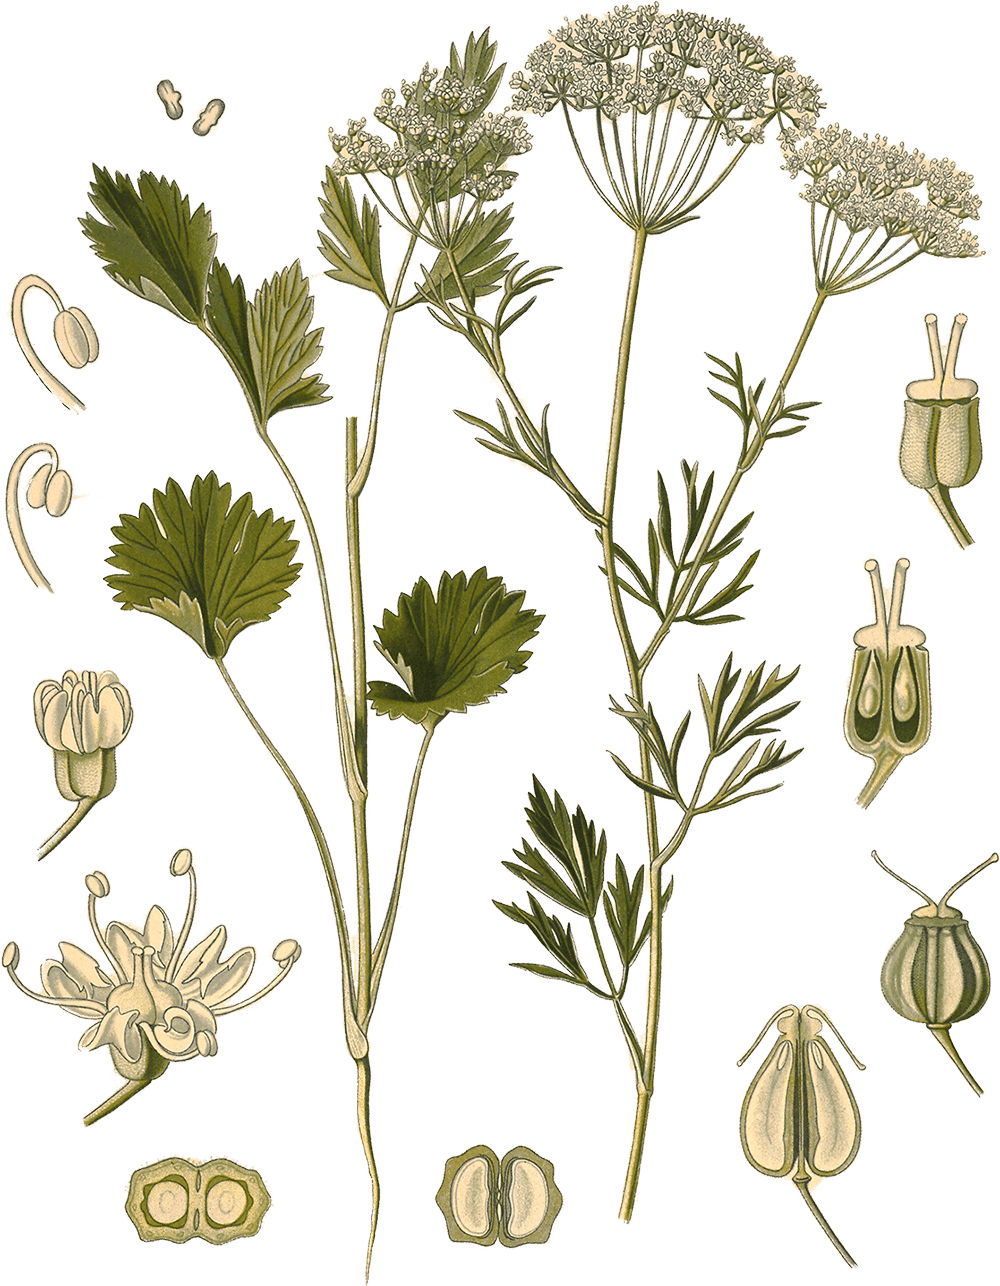
\includegraphics[width=\textwidth]{imgs/kohler/anise_kohler_min.png}
%     \caption{\taxonn{Pimenta dioica}{(L.) Merr.} (syn. \taxonn{P. officinalis}{ Lindl.}), the allspice tree in Köhler's Medicinal Plants \pvolcite[]{2}[174]{kohler_kohlers_1887}.}
%     \label{fig:kohler_anise}
% \end{figure}



\section{Anise}
\label{sec:anise}

\begin{spice}\label{spice:anise}
\textsc{Anise} \hfill \href{https://powo.science.kew.org/taxon/846658-1}{POWO} \\
\textbf{English:} \textit{anise}; \textit{aniseed}. 
\textbf{Arabic:} {\arabicfont{أنيسون}} \textit{anīsūn}; {\arabicfont{{يانسون} \textit{yānsūn}}}. 
\textbf{Chinese:} {\tradchinesefont{茴芹}} \textit{huíqín} [anise-celery]. 
\textbf{Hungarian:} \textit{ánizs}.  \\
\noindent{\color{black}\rule[0.5ex]{\linewidth}{.5pt}}
\begin{tabular}{@{}p{0.25\linewidth}@{}p{0.75\linewidth}@{}}
Plant species: & \taxonn{Pimpinella anisum}{L.} \\
Family: & \textit{Apiaceae} \\
part used: & fruit; oil \\
Region of origin: & E. Mediterranean; W. Asia \\
Cultivated in: & Turkey; Egypt; Spain; Russia; Italy; etc. \\
Color: & light brown \\
\end{tabular}
\end{spice}

% \begin{figure}[!ht]
% 	\vspace{-4ex}
% 	\centering
% 	\subfloat[\centering]{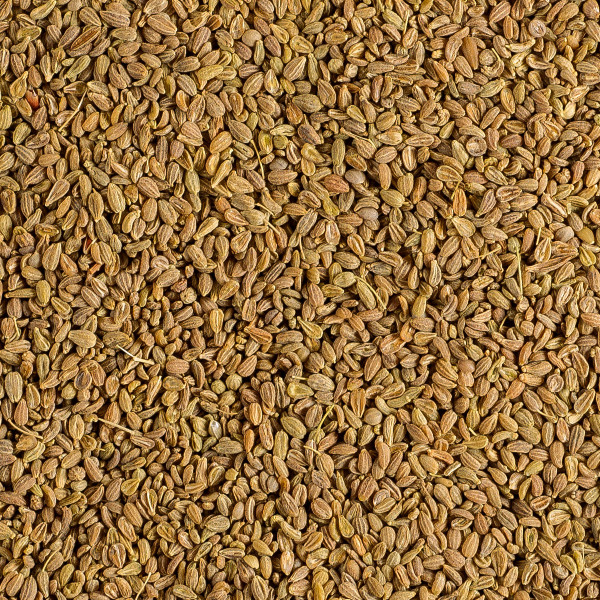
\includegraphics[width=0.3\linewidth]{imgs/spices/anise-1.jpg}}
% 	\hfill
% 	\subfloat[\centering]{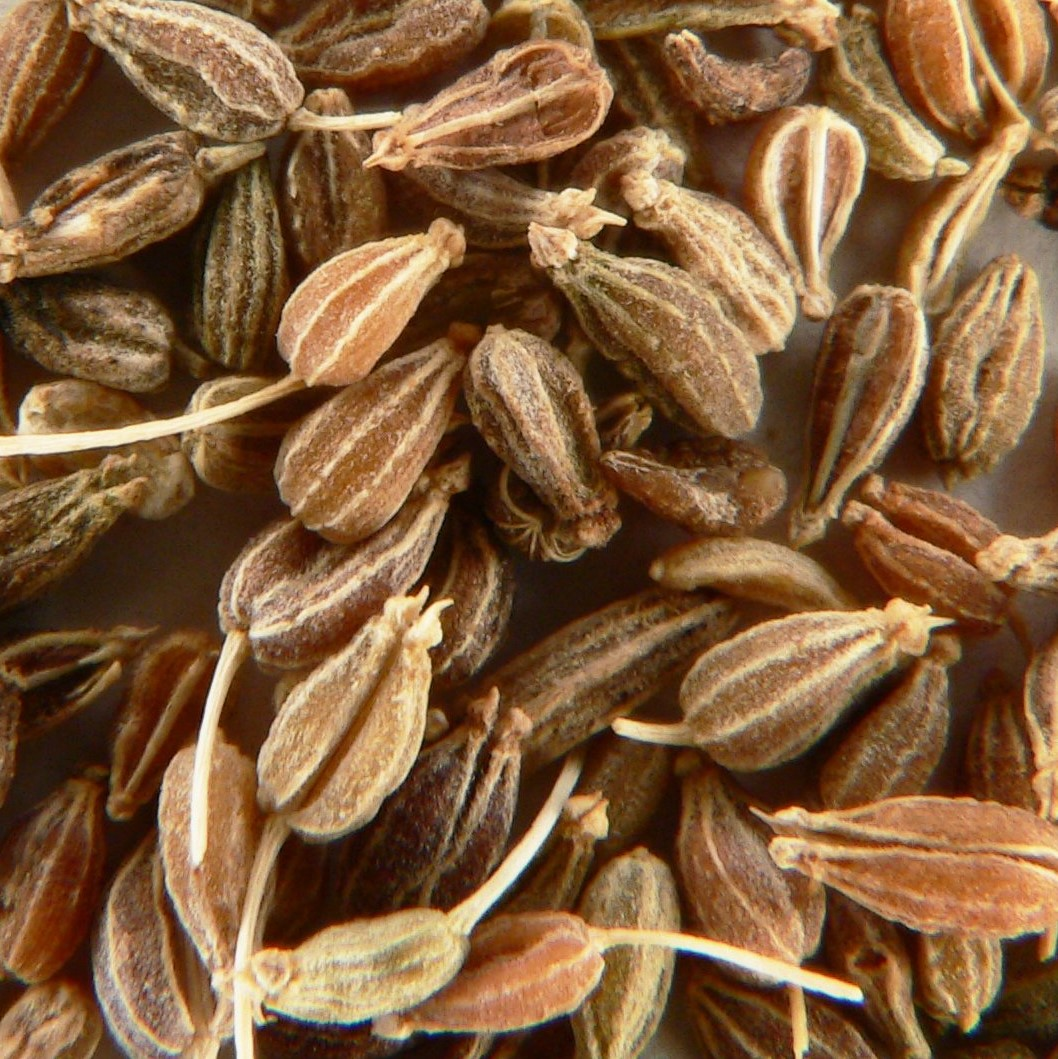
\includegraphics[width=0.3\linewidth]{imgs/spices/anise-11.jpg}}
% 	\hfill
% 	\subfloat[\centering]{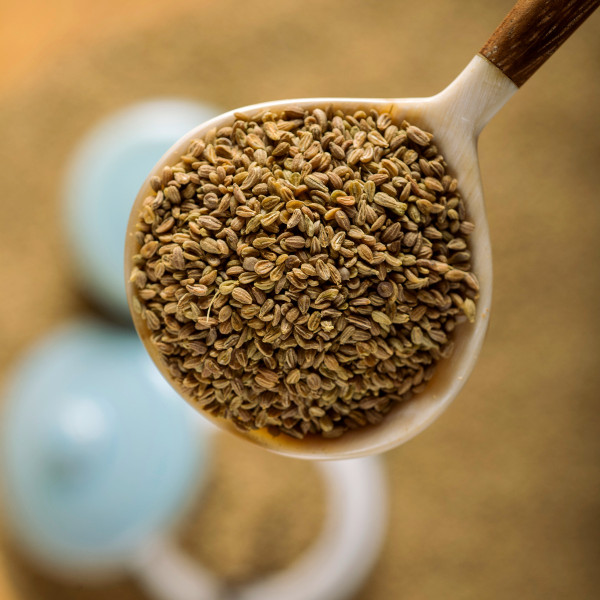
\includegraphics[width=0.3\linewidth]{imgs/spices/anise-3.jpg}}
% 	\caption{Anise \textit{Pimpinella anisum}.}
% 	\label{fig:anise_imgs}
% \end{figure}

\begin{wrapfigure}{R}{0.33\textwidth}
	\vspace{-\baselineskip}
	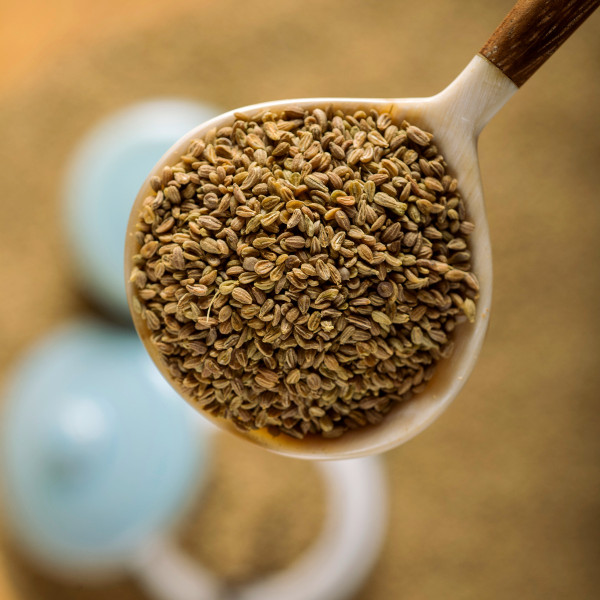
\includegraphics[width=0.33\textwidth]{imgs/spices/anise-s.jpg}
	\caption{Anise ``seeds'' (\textit{Pimpinella anisum}).}
	\label{fig:anise}
\end{wrapfigure}

%DESCRIPTION

Anise (\textit{Pimpinella anisum}) is a herbaceous plant, native to the Eastern Mediterranean and the Levant. It yields downy schizocarps,\footnote{Schizocarp refers to a dry compound fruit which splits into two or more one-seeded carpels (mericarps) without dehiscing} fruits which people call seeds. Hence the popular contracted form of the name, \textit{aniseed}. The seed-like fruits are grayish-green to light brown in color, and around 3--6 mm long \autocite[212]{van_wyk_culinary_2014}. Commercially available anise is usually sold whole, with a bit of stalk attached. Anise has visible \textit{vittae} (oil ducts) embedded in the fruit wall \pvolcite[]{2}[139]{peter_handbook_2012}, which is a feature similarly found on the fruits of related umbelliferous aromatic plants, such as fennel, cumin, caraway, carom/ajwain, and dill seeds.
Anise is sought after for its characteristic, liquorice-like sweet aroma and flavor, used in gastronomy, confectionery, and liqueur making -- especially around the Mediterranean. 
Anise and its essential oil is traditionally used as a flavoring for food, candy, and alcoholic drinks, however star anise oil from China has gradually replaced anise oil in the industry thanks to it being a much cheaper substitute \autocite[212]{van_wyk_culinary_2014}. % By 1999, world production in essential oil obtained from anise was 8 tons, while that of star anise was 400 \autocite{ashurst_food_1999}.

%OPERATIVE
The taste, smell, and even the appearance of anise resembles other---related and unrelated---spices, such as fennel, dill, liquorice, and star anise. This leads to a certain degree of confusion around the names which these plants and their products are known today in various languages. We will introduce this problem in more detail in \cref{sec:case_star_anise} in \nameref{ch:language}.

\begin{note}
	It is important to make the distinction between anise (\textit{Pimpinella anisum}) and star anise (\textit{Illicium verum}) from the beginning. These are two unrelated spices with distant origins. The similarities in name are due to their similarity in flavor, thanks to the organic compound anethole. 
	\end{note}

\subsection{The Botany, Origin, and  Cultivation of Anise}

%PLANT
Anise is an annual herb from the family \textit{Apiaceae/Umbelliferae}. Growing less than a meter tall, it brings small white flowers in umbels, the shape of an umbrella which is typical for this family of parsley, celery, and carrot. This family also contains many other aromatic flowering plants, such as asa\-foetida, coriander, cumin, caraway, dill, and fennel.

%ORIGIN
Anise originates in the Eastern Mediterranean region, growing from South East Turkey through Syria to the coasts of Lebanon, Israel, Palestine, and Egypt, including Cyprus, and in some sources also Greece. It has been cultivated since 2000 \BC{} \autocite[718]{mabberley_mabberleys_2017}.
%CULT
Anise today is naturalized in most of Europe and Central Asia, and it is cultivated as a crop in various regions around the globe, including, Southern Europe, Southern Russia, Turkey, the Middle East and North Africa, Pakistan, India, China, Chile, Mexico and the United States \autocite[32]{farrell_spices_1985}. It requires good soil, lots of sun and warmth, and also arduous to transplant. During harvest at summer's end when the fruits begin to ripen, the plant parts above ground are cut and the ``seeds'' are dried \autocite[212]{van_wyk_culinary_2014}.

\subsection{The History of Anise}

Anise has a long history around the Mediterranean, and its popularity is still concentrated there. It was used both as medicine an a culinary spice, as I mentioned above. The ancient Greeks took it as a breath freshener, and the Romans used it in their cooking \autocite{farrell_spices_1985}.

Pliny wrote a section of remedies with anise in his \textit{Natural History}, where he explains that it was recommended by Pythagoras to take with wine against scorpion stings, but it is also a great ingredient---both green and dried---in sauces and breads. And of course, it sweetens the morning breath with a little honey and smyrnion\footnote{\textit{Smyrnium olusatrum}, an edible pot herb commonly known as \textit{alexanders}} \autocite[20:72 \link{http://www.perseus.tufts.edu/hopper/text?doc=Perseus\%3Atext\%3A1999.02.0137\%3Abook\%3D20\%3Achapter\%3D72}]{pliny_the_elder_natural_1855}.

Medieval European herbals tell of carminative effect: ``The seed wasteth and consumeth winde, and is good against belchings and upbraidings of the stomach, alaieth gripings of the belly, provoketh urine gently, maketh abundance of milke, and stirreth up bodily lust: it staieth the laske (diarrhea), and also the white flux (leukorrhea) in women.'' \autocite[880 \link{https://www.gbif.org/species/113561272}]{gerarde_herball_1597}. Based on modern research, anise oil and anethole is antibacterial, antifungal, antioxidant, carminative, and expectorant \pvolcite[]{2}[144]{peter_handbook_2012}.

The Brits and Arabs use it since the Middle Ages. According to \textcite{wilson_wedding_2005}, 
the tradition of the wedding cake grew out of the customary spiced cakes at the end of feasts during Roman times, which served as digestive. In modern Europe, its use is prevalent in confectionery (such as aniseed balls), but especially liqueurs. From the many Mediterranean alcoholic beverages flavored with anise, we can mention anisette and absinthe (made with \textit{Artemisia absinthium}), from France, sambuca from italy, and ouzo and mastika from Greece. 
% ouzo effect
In the Eastern Mediterranean, it can be found in Turkish rakı, and the many araks of the Levant.

% USES
% culinary uses wyk
% Anise has a strong flavour and is used sparingly as a spice in soufflés, meat dishes (soups, stews, sausages), shellfish, vegetables (cabbage, carrots, turnips), mild cheeses, salad dressings, pickles, fruit dishes, desserts and juices. Chopped fresh leaves can be used in salads, pickled vegetables and fish soups. Star anise is nowadays often used as a substitute but connoisseurs say anise has a more delicate aroma. Anise is well known for its applications in confectionery (breads, biscuits, cakes and sweets) as well as alcoholic and non-alcoholic beverages. Examples of traditional culinary items and sweets are Australian humbugs, Austrian anisbögen, British aniseed balls, Dutch muisjes, German Pfeffernüsse and Springerle, Indian candy-coated saunf (used as mukhwas to freshen the breath after a meal), Italian pizzelle, New Mexican bizcochitos, New Zealand aniseed wheels, Norwegian knotts and Peruvian picarones. Well-known anise liqueurs or brandies/liquors (i.e., respectively with or without sugar) include French anisette, pastis and Pernod, Greek ouzo, Middle Eastern arrack, Italian sambuca, Spanish anís and Turkish raki. These are drunk with a glass of water on the side or more often directly diluted with water, resulting in the familiar ouzo effect (the drink becomes cloudy and milky because the alcohol-soluble anethole is no longer fully soluble and forms an emulsion). 

%Flavour compounds
%The fruits contain 1−4% essential oil with (E)-anethole, also referred to as trans-anethole, as the dominant compound (up to 90% or more) and several minor ingredients such as cis-γ-himachalene, trans-pseudoisoeugenyl 2-methylbutyrate, methylchavicol and p-anisaldehyde.3 Anethole is a phytoestrogen that also occurs in fennel. 

%notes In Pakistani and Indian cuisine, no distinction is made between anise and fennel – both are called saunf. In Southeast Asia, the name for star anise is sometimes shortened to anis.

% Mebberley:
% P. anisum L. (anise, Greece to Egypt) – cult. since 2000 BC, food& drink-flavouring subs. for Artemisia absinthium (absinthe, anis, anisette, arak, ouzo, pastis, raki), distilled oil medic., familiar as aniseed balls;

\subsection{The Names of Anise}

\textit{Anise} is a typical \gls{wanderwort}: emerging from moderately obscure origins, it is now ubiquitous to the languages of Europe and its sphere of influence where it is culturally significant.

\subsubsection{English}

\begin{etymology}\label{ety:anise}
English \textit{anise}, ca. 1325
< French \textit{anis} `anise', 1236
< Latin \textit{anīsum} `anise', (dill is \textit{anēthum})
< Ancient Greek {ἄνισον} \textit{ánison} `anise; dill', and other Greek dialectal variants, e.g.: \textit{ánēthon}; included both plants, only later distinguished (probaby of substrate origin)
<\textss{?} Egyptian (Ancient) \textit{jnst} `a medicinal, edible plant (probably anise)'\footnote{\textcites[anise]{oed}[anise]{ahd}; \textcite[s.v. anis]{tlfi}; \textcite{lewis_latin_1879}; \textcite{liddell_greek-english_1940}; \textcites[99]{erman_worterbuch_1926}[240]{hemmerdinger_noms_1968}}
\end{etymology}

To English, it arrived in the \nth{14} century via French \textit{anis}, which descended from Latin \textit{anīsum}. The Latin word is a borrowing from Ancient Greek ἄνισον \textit{ánison}, which is attested in different forms in various Greek dialects of the time, sometimes with \textit{-nn-} and theta instead of sigma (e.g.,ἄνηθον \textit{anēthon}). We can often read that this word originally referred to dill, but it seems that the Greeks did not distinguish between the two, and the terms included both plants.\footcite[anise]{oed} Hence the scientific name of dill: \textit{Anethum graveolens}. According to \textcite[103,107]{beekes_etymological_2010}, \textit{ánison} is anise, while \textit{anēthon} is dill, but he points out that they probably have the same etymon. The Romans borrowed both words, and the distinction was made explicit in \textit{anīsum} vs. \textit{anēthum}. The modern scientific names bear the Latin names: \textit{Pimpinella anisum} (anise), where meaning of \textit{pimpinella} is uncertain, and \textit{Anethum graveolens} (dill), where \textit{graveolens} means `strong scented' \autocite[184,303]{gledhill_names_2008}. The confusion of the Greek words had an effect on English much later as well, in Matthew 23:23 of the \gls{KJV}\footnote{Source: \url{https://www.biblegateway.com/passage/?search=Matthew+23\%3A23&version=KJV}} talks of anise, while newer, more accurate translations, such as the \gls{NRSV}\footnote{Source: \url{https://www.biblegateway.com/passage/?search=Matthew+23\%3A23&version=NRSVUE}} mention dill. In fact, one of the first attestation in English comes from Wycliffe's Bible in 1382, between mint and cumin: ``That tithen mente, anete [anese], and comyn.''\footcite[anise]{oed} Beyond Greek, the etymology of this word is uncertain, \textcite[103,107]{beekes_etymological_2010} suspects a pre-Greek, substrate origin demonstrated by the phonological variations. Although the \citetitle{erman_worterbuch_1926} in an early Egyptian glossary makes a connection with the Egyptian word rendered as \textit{jnst}\footnote{Transliterated as \textit{ꞽnś.t} in \textcite[99]{erman_worterbuch_1926}, conventional Egyptological pronunciation: /insɛt/} `an edible plant for medicinal use' in the literature of the Middle Kingdom, the assumption is marked with question marks in the original handwritten glossary \autocites[240]{hemmerdinger_noms_1968}[99]{erman_worterbuch_1926}. The \gls{AHD} remarks that the Greek word is ``perhaps from or akin'' to Egyptian \textit{ꞽnśt}---using a different transliteration---which is a kind of plant used in the preparation of refreshing drinks, possibly anise.\footcite[anise \link{https://www.ahdictionary.com/word/search.html?q=anise}]{ahd} 

% An association between dill and the ancient city of Imsety has been made due to the similarity of their names in Old Egyptian. Redford 1:562; more about jnst in Wiktionary

The idea is not far-fetched, anise, dill and other herbs are native to the region and were ``almost surely grown'' for their medicinal properties \pvolcite[]{2}[3]{redford_oxford_2001}. We know that spices and herbs were used to flavour Ancient Egyptian cooking, Egyptologists have identified indigenous ingredients (dill, fenugreek, parsley, thyme, nigella, fennel, marjoram, mint), those imported and transplanted from neighboring Palestine (dill, cumin, coriander, caraway) and those obtained through distant trade (cinnamon and peppercorns from Asia) by the wealthy, later during the New Kingdom times \pvolcite[]{1}[394,540]{redford_oxford_2001}.

Anise is also known as \textit{aniseed}, which is a contraction from \textit{anise} and \textit{seed}, a usage form that emerged in the late \nth{14} century. 

\textit{Sweet cumin} is another conventional name for anise, which shows the primacy of the word \textit{cumin} in English, when it comes to similar aromatic plants and their seeds. Cf. \textit{wild cumin}, \textit{Armenian cumin}, \textit{mountain cumin} (caraway); royal cumin\footnote{Parallel to Indo-Persian \textit{sh\={a}h-j\={i}r\={a} [king-cumin] `caraway'}} (bishop's weed), and the always ambiguous \textit{black cumin}

\begin{table}[!ht]
\centering
\begin{tabularx}{\textwidth}{@{}l>{\itshape \small}lL>{\small}l@{}}
\toprule
\textbf{\#} & \multicolumn{1}{l}{\textbf{Species}} & \multicolumn{1}{l}{\textbf{Name}} & \multicolumn{1}{l}{\textbf{Source}} \\
\midrule
\textbf{1}	& \textbf{Pimpinella anisum}	& \textbf{anise}	& \textbf{\textcite{van_wyk_culinary_2014}} \\
2	& Pimpinella anisum	& aniseed	& \textcite{van_wyk_culinary_2014} \\
3	& Pimpinella anisum	& sweet cumin	& \textcite{peter_handbook_2012} \\
\bottomrule
\end{tabularx}
\caption{Various names for anise in English.}
\label{table:names_anise_en}
\end{table}



\subsubsection{Arabic}

\begin{etymology}\label{ety:anisun}
Arabic {أنيسون} \textit{anīsūn} `anise', (later assimilated as \ar{يانسون} \textit{yānsūn}), a. 791
< Ancient Greek {ἄνισον} \textit{ánison} `anise; dill', and other Greek dialectal variants, e.g.: \textit{ánēthon}; included both plants, only later distinguished (probaby of substrate origin)
<\textss{?} Egyptian (Ancient) \textit{jnst} `a medicinal, edible plant (probably anise)', ca. 2030-1650 BC\footnote{\textcite{wehr_dictionary_1976}; \textcite{liddell_greek-english_1940}; \textcites[99]{erman_worterbuch_1926}[240]{hemmerdinger_noms_1968}}
\end{etymology}

In Arabic, similarly to English, the name of anise is a loanword from Greek. It is known by many spelling variations: \textit{anīsūn}, \textit{ānīsūn}, \textit{ansūn}, \textit{yānsūn}, and \textit{yansūn}. In general, the \textit{a-} forms were the initial loanword taken directly from Greek, then a \textit{y-} form emerged that assimilates better in Arabic phonology. In addition, synonyms for anise are \textit{kammūn ḥulw}, lit. `sweet cumin', and \textit{ḥubba ḥulwa} `sweet grain, sweet seed'.

Anise in Persian, is \fa{بادیان رومی} \textit\textit{bādyān rūmī}\footcite[Vol. 1, p. 197]{hayyim_new_1934}, literally `Roman anise', where \textit{bādyān} is an archaic word for either fennel or anise, the etymon of French \textit{badiane} that begot English \textit{badian} `star anise'. A possible connection between Persian \textit{bādyān} and Mandarin Chinese \tc{八角} \textit{bajiao} `star anise' have been proposed before, % by who
but in my opinion this is merely wishful thinking.

\begin{table}[!ht]
\centering
\begin{tabularx}{\textwidth}{@{}l>{\itshape \small}lr>{\itshape}lL>{\small}l@{}}
\toprule
\textbf{\#} & \multicolumn{1}{l}{\textbf{Species}} & \multicolumn{1}{l}{\textbf{Name}} & \multicolumn{1}{l}{\textbf{Tr.}} & \multicolumn{1}{l}{\textbf{Gloss}} & \multicolumn{1}{l}{\textbf{Source}} \\
\midrule
\textbf{1}	& \textbf{Pimpinella anisum}	& \textbf{أنيسون}	& \textbf{anīsūn}	& \textbf{phonetic}	& \textbf{\textcite{wehr_dictionary_1976}} \\
2	& Pimpinella anisum	& كمون حلو	& kammūn ḥulw	& sweet cumin	& \textcite{wehr_dictionary_1976} \\
3	& Pimpinella anisum	& يانسون	& yānisūn	& phonetic	& \textcite{wehr_dictionary_1976} \\
4	& Pimpinella anisum	& حبة حلوة	& ḥabba ḥulwa	& sweet grain, seed	& \textcite{wehr_dictionary_1976} \\
\bottomrule
\end{tabularx}
\caption{Various names for anise in Arabic.}
\label{table:names_anise_ar}
\end{table}



\subsubsection{Chinese}

\begin{etymology}\label{ety:huiqin}
Mandarin Chinese {茴芹} \textit{huíqín} `anise' [hui-celery], from \textit{hui} `anise/fennel' + \textit{qin} `celery' (茴 \textit{huí} could be interpreted as `Muslim spice', see 茴香 \textit{huíxiāng} `fennel'), 1841\footnote{\textcite{kleeman_oxford_2010; hu_food_2005}}
\end{etymology}

The gathering of names for anise is a bit difficult in Chinese for two reasons. Firstly, anise as a spice is relatively unknown in China except for Xinjiang, and therefore names are hard to find in sources. Since other spices with a similar flavour profile, such as the native star anise and the naturalized fennel are readily available, so anise was never imported into China. Consequently, we cannot find anise in reference works on Chinese food plants nor in Chinese \gls{materia medica} \autocite[see][]{hu_enumeration_1999, hu_food_2005}. It does however appear in the \gls{FOC}\footnote{Source: \url{http://www.efloras.org/florataxon.aspx?flora_id=2&taxon_id=200015767}} Secondly, identifications is problematic and confusing due to the mixing of terms \textit{anise}, \textit{aniseed}, \textit{star anise}, \textit{star aniseed}, etc. in English, and Chinese dictionaries, and in some databases as well. Dictionaries that do not give botanical names are of little help to clarify doubts, but some conclusions can be derived with care. Most dictionary entries in Chinese that translate \textit{anise} to \textit{aniseed} should in fact say \textit{star anise}, as they ar all words referring to the Asian spice, except for one: \tc{茴芹} \textit{huiqin}.

Anise in Chinese is 茴芹 \textit{huiqin} `anise-celery', which appears to be a relatively modern, scientific coinage, and the only \gls{phytonym} that appears in any publication (the \gls{FOC}). It is used in the strict sense of \textit{Pimpinella anisum} and cannot be misunderstood for star anise (\textit{Illicium verum}). It does not appear in historical corpora, and it is not included in the \nth{7} edition of the \textit{Xiandai Hanyu Cidian} [A Dictionary of Modern Chinese] \autocite[]{chinese_academy_of_social_sciences_xiandai_2016}, but it appears in the \gls{CEC}\footnote{Source: \url{https://dictionary.cambridge.org/dictionary/english-chinese-traditional/anise} and \url{https://dictionary.cambridge.org/dictionary/english-chinese-traditional/aniseed}.}, which gives us \textit{huiqin}, along with \tc{洋茴香} \textit{yanghuixiang} `Western anise'. \tc{茴香} \textit{huixiang} really refers to fennel, and the only reason it appears in \textcite{kleeman_oxford_2010} is the confusion between the materials, and their names. The nomenclature and the reasons behind its confusion will be explored in more detail in \cref{sec:case_star_anise}. A few other names are mentioned on the Chinese Wikipedia page of the plant, these all refer to the European origins of this spice, or referring to``Western Ocean'', the Indian Ocean used to denote foreign, western products that have arrived over sea.\footnote{Source: \url{https://zh.wikipedia.org/wiki/\%E8\%8C\%B4\%E8\%8A\%B9}}. 

A Latin-Chinese dictionary from a presbyterian missionary from 1841 lists \textit{huiqin} as \textit{thymus} `thyme',\footcite[715]{goncalves_lexicon_1841} which is rather confusing considering that 10 years earlier, the same author rendered it `oregano' in his Portuguese-Chinese dictionary.\footcite[585]{goncalves_diccionario_1831}. From this, we can speculate that more of the various spice herbs that the Portuguese and other Europeans brought to Macao were first denoted with \textit{huiqin}.

% oregano in 
% https://books.google.com.hk/books?id=BYE-AQAAIAAJ&pg=PA585&dq=%22%E8%8C%B4%E8%8A%B9%22&hl=en&sa=X&ved=2ahUKEwi1xs7slpb5AhWJet4KHe9NCicQ6AF6BAgEEAI#v=onepage&q=%22%E8%8C%B4%E8%8A%B9%22&f=false

% thyme in
% https://books.google.com.hk/books?id=rOBoAAAAcAAJ&pg=PA715&dq=%22%E8%8C%B4%E8%8A%B9%22&hl=en&sa=X&ved=2ahUKEwi1xs7slpb5AhWJet4KHe9NCicQ6AF6BAgJEAI#v=onepage&q=%22%E8%8C%B4%E8%8A%B9%22&f=false

\begin{table}[!ht]
\centering
\begin{tabularx}{\textwidth}{@{}l>{\itshape \small}ll>{\itshape}lL>{\small}l@{}}
\toprule
\textbf{\#} & \multicolumn{1}{l}{\textbf{Species}} & \multicolumn{1}{l}{\textbf{Name}} & \multicolumn{1}{l}{\textbf{Tr.}} & \multicolumn{1}{l}{\textbf{Gloss}} & \multicolumn{1}{l}{\textbf{Source}} \\
\midrule
\textbf{1}	& \textbf{Pimpinella anisum}	& \textbf{\tradchinesefont{茴芹}}	& \textbf{huíqín}	& \textbf{hui-celery}	& \textbf{\textcite{kleeman_oxford_2010}} \\
2	& Pimpinella anisum	& \tradchinesefont{茴香}	& huíxiāng	& hui-spice	& \textcite{kleeman_oxford_2010} \\
3	& Pimpinella anisum	& \tradchinesefont{西洋茴香}	& xīyánghuíxiāng	& western-ocean-hui-spice	& \textcite{wikipedia} \\
4	& Pimpinella anisum	& \tradchinesefont{洋茴香}	& yánghuíxiāng	& ocean-hui-spice	& \textcite{cec} \\
5	& Pimpinella anisum	& \tradchinesefont{歐洲大茴香}	& ōuzhōu dàhuíxiāng	& European-big-hui-spice	& \textcite{wikipedia} \\
\bottomrule
\end{tabularx}
\caption{Various names for anise in Chinese.}
\label{table:names_anise_zh}
\end{table}



\subsubsection{Summary}

\Cref*{table:names_anise} shows the names of anise that can be found in dictionaries.

\begin{table}[!ht]
\centering
\begin{tabularx}{\textwidth}{@{}ll>{\itshape}lLl>{\small}l@{}}
\toprule
\textbf{\#} & \textbf{Language} & \multicolumn{1}{l}{\textbf{Term}} & \textbf{Gloss} & \textbf{Loan} & \multicolumn{1}{l}{\textbf{Source}} \\
\midrule
1	& English	& anise	& 	& yes	& \textcite{oed} \\
2	& English	& aniseed	& 	& no	& \textcite{oed} \\
3	& English	& sweet cumin	& 	& no	& \textcite{oed} \\
\midrule
1	& Arabic	& anīsūn	& phonetic	& yes	& \textcite{wehr_dictionary_1976} \\
2	& Arabic	& kammūn ḥulw	& sweet cumin	& no	& \textcite{wehr_dictionary_1976} \\
3	& Arabic	& yānisūn	& phonetic	& yes	& \textcite{wehr_dictionary_1976} \\
4	& Arabic	& ḥabba ḥulwa	& sweet grain, seed	& no	& \textcite{wehr_dictionary_1976} \\
\midrule
1	& Chinese	& huíqín	& hui-celery	& no	& \textcite{kleeman_oxford_2010} \\
2	& Chinese	& huíxiāng	& hui-spice	& no	& \textcite{kleeman_oxford_2010} \\
\bottomrule
\end{tabularx}
\caption{Conventionalized names for anise in English, Arabic, and Chinese, found in dictionaries.}
\label{table:names_anise}
\end{table}













%==========================================

% EE:
% umbelliferous plant with aromatic seeds. XIV. — (O)F. anis :- L. ánīsum — Gr. ānīson.
% Hence aniseed XIV (anece seed).

% OE:
% anise (n.)
% Levantine plant cultivated for its seeds, which were important sources of chemical oils and flavoring, c. 1300, from Old French anis (13c.), from Latin anisum, from Greek anison. By the Ancients somewhat confused with dill. Related: Anisic.
% Entries linking to anise
% aniseed (n.)
% late 14c., a contraction of anise seed (n.).
% anisette (n.)
% "liqueur flavored with aniseed," 1821, from French Anisette de Bordeaux, from diminutive of anis (see anise).

% MW:
% Middle English anis, from Old French, from Latin anisum, anesum, from Greek anison, anēson
% First Known Use: 14th century (sense 1)

% AH:
% [Middle English anis, from Old French, from Latin anīsum, from Greek annēson, annīson, anīson; akin to anēthon, annēthon, dill, and perhaps from or akin to Egyptian jnś.t, a kind of plant used in preparing refreshing drinks (possibly anise).] 

% WK:
% From Middle English anys, borrowed from Old French anis, from Latin anīsum, from Ancient Greek ἄνισον (ánison), from Egyptian jnst. 

\clearpage % % Full page illustration
% \begin{figure}[!hbtp]
%     \centering
%     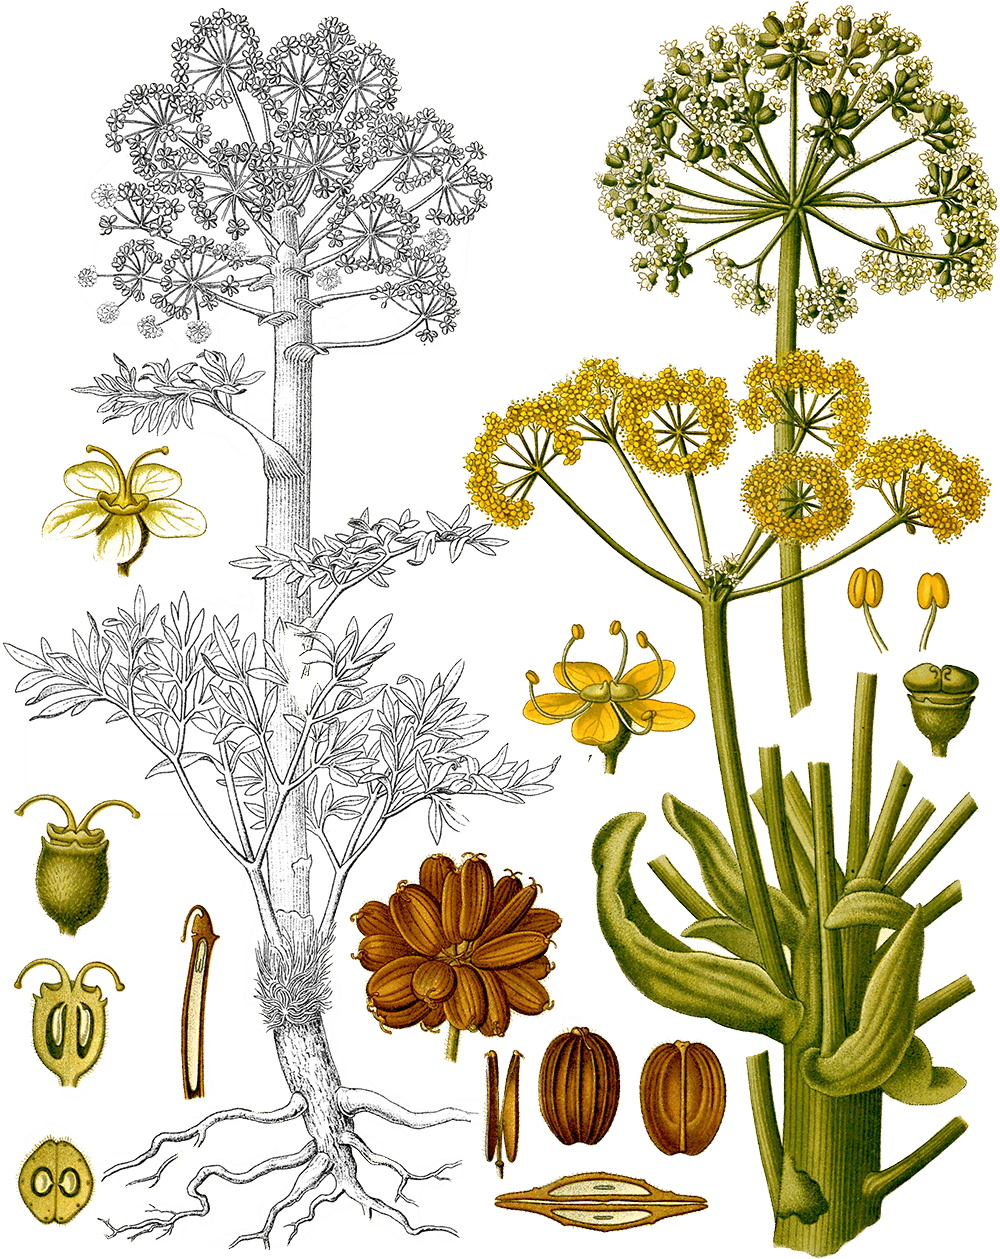
\includegraphics[width=\textwidth]{imgs/kohler/asafoetida_kohler_min.png}
%     \caption{\taxonn{Ferula foetida}{(Bunge) Regel} (syn. \taxonn{Ferula scorodosma}{Benth. \& Hook.}), one of the sources of asafoetida in Köhler's Medicinal Plants \pvolcite[]{2}[147]{kohler_kohlers_1887}.}
%     \label{fig:kohler_asafoetida}
% \end{figure}



\section{Asafoetida}
\label{sec:asafoetida}

\begin{spice}\label{spice:asafoetida}
\textsc{Asafoetida} \hfill \href{https://powo.science.kew.org/taxon/842277-1}{POWO} \\
\textbf{English:} \textit{asafoetida}; \textit{hing; devil's dung}. 
\textbf{Arabic:} {\arabicfont{حلتیت}} \textit{ḥiltīt}. 
\textbf{Chinese:} {\tradchinesefont{阿魏}} \textit{āwèi}. 
\textbf{Hungarian:} \textit{ördöggyökér} [devil's root]; \textit{aszatgyanta} [asat resin]; \textit{bűzös aszat} [stinking asat].  \\
\noindent{\color{black}\rule[0.5ex]{\linewidth}{.5pt}}
\begin{tabular}{@{}p{0.25\linewidth}@{}p{0.75\linewidth}@{}}
Plant species: & \taxonn{Ferula foetida}{(Bunge) Regel}; \textit{\taxonn{Ferula assa-foetida}{L.}; \textit{Ferula narthex}; et al.} \\
Family: & \textit{Apiaceae} \\
part used: & gum-resin (latex) \\
Region of origin: & Iran; W. and C. Asia \\
Cultivated in: & Iran; Afghanistan \\
Color: & from pale yellow to brown \\
\end{tabular}
\end{spice}

\begin{figure}[!ht]
	\vspace{-4ex}
	\centering
	\subfloat[\centering gum-resin ]{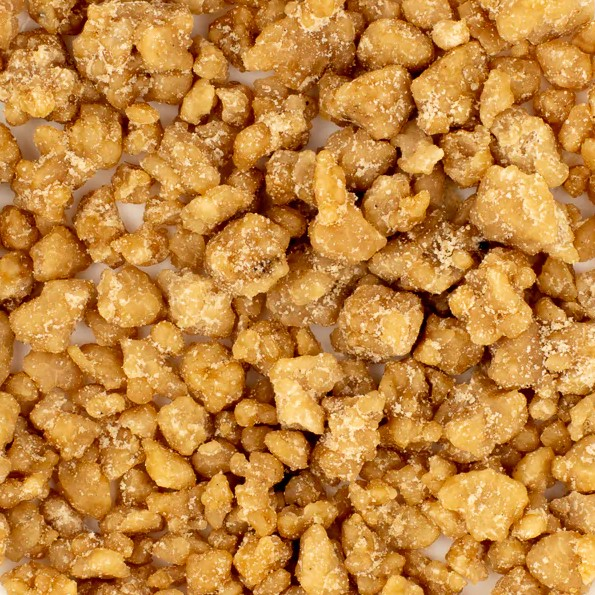
\includegraphics[width=0.3\linewidth]{imgs/spices/asafoetida-1.jpg}}
	\hfill
	\subfloat[\centering powder, colored with turmeric]{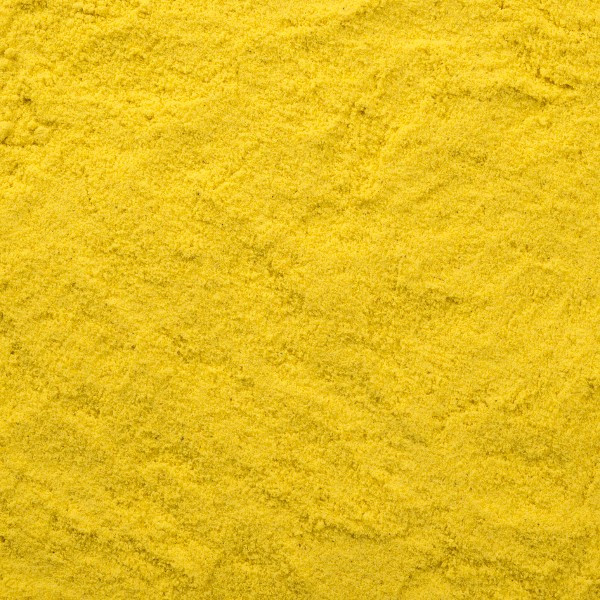
\includegraphics[width=0.3\linewidth]{imgs/spices/asafoetida-2.jpg}}
	\hfill
	\subfloat[\centering plant]{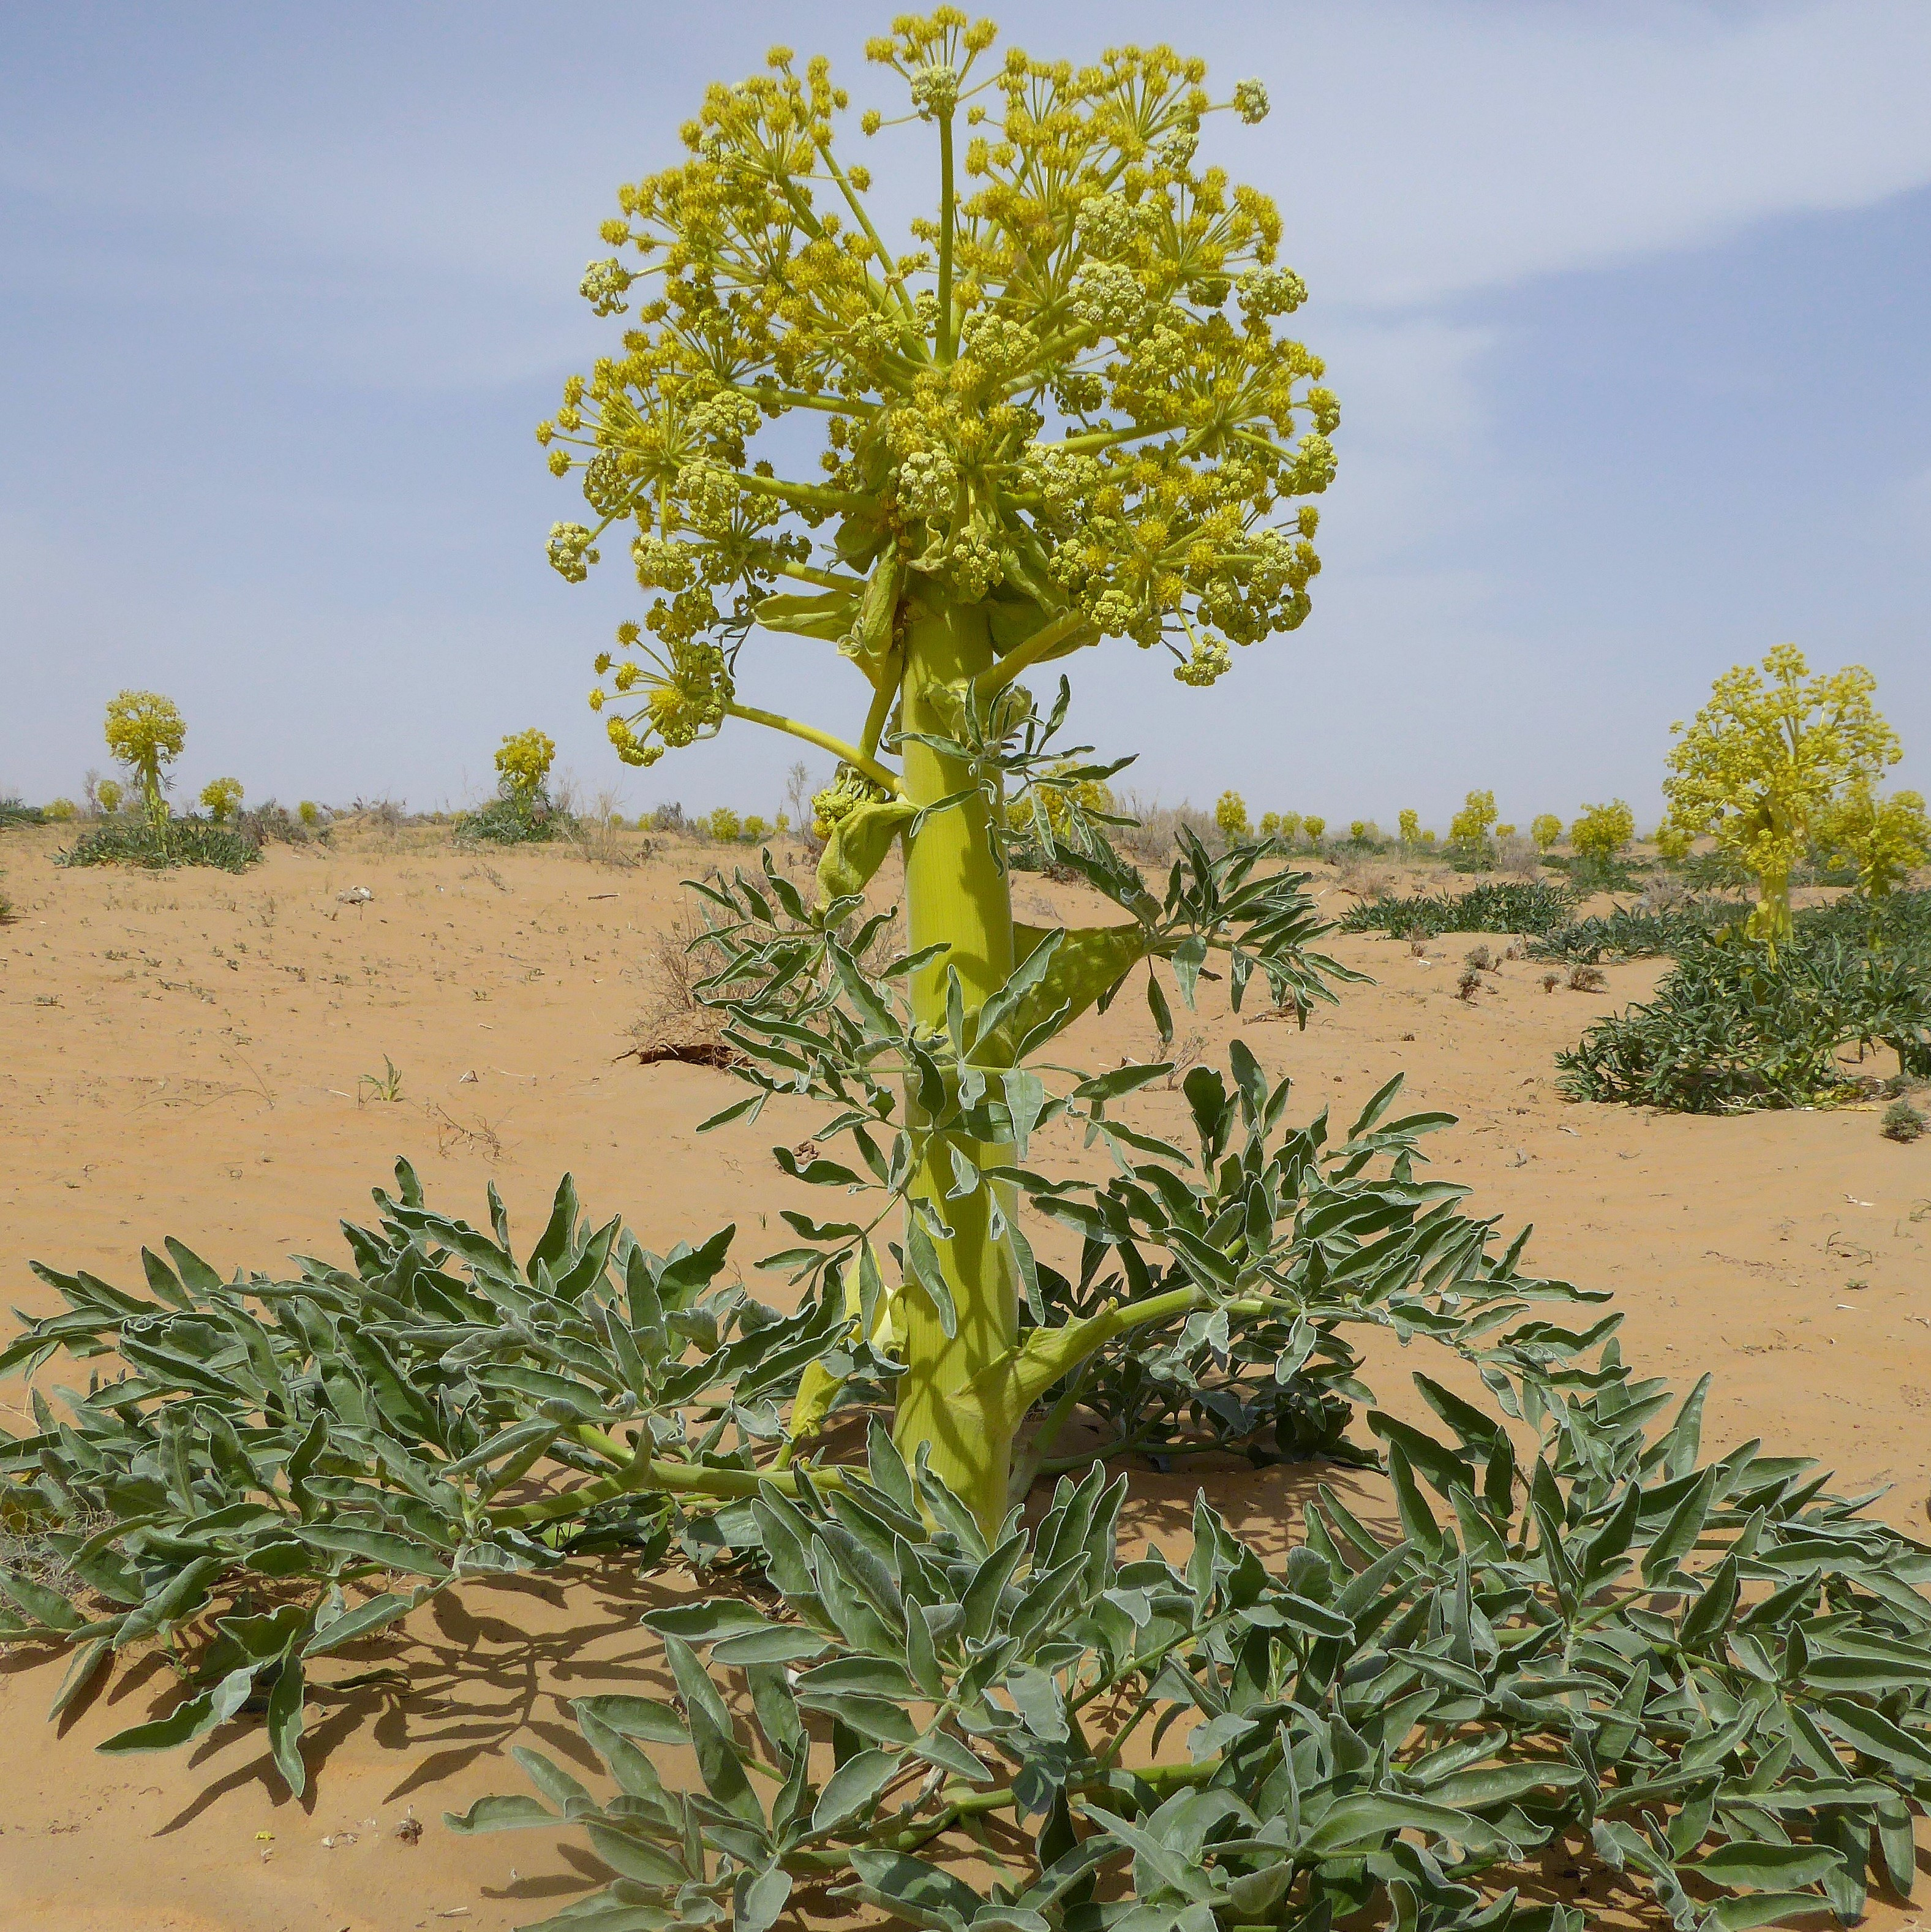
\includegraphics[width=0.3\linewidth]{imgs/spices/asafoetida-3.jpg}}
	\caption{Asafoetida in various forms, and one of its principal sources \taxon{Ferula assa-foetida} in the Kyzylkum Desert. Credit: Glorian; Aromatique; Public Domain}
	\label{fig:asafoetida_imgs}
\end{figure}

Asafoetida is the dried, golden brown oleoresin that forms after cutting the stems of various ferula plants of Central Asia. The material itself is a waxy gum-resin, and it is sold either in gum or powdered form. Asafoetida is an extremely pungent, strong-smelling substance; it is described having a ``garlic-like'' and ``sulphurous odor'' that is sometimes too strong in itself and must be diluted with other materials \autocite[138]{van_wyk_culinary_2014}. Asafoetida is a drug and spice, and was used for centuries in both Asia and Europe \autocite{leung_itinerary_2019}. It is still an integral part of Indian cuisine as an ingredient, while in Europe and East Asia it was mainly utilized as medicine.

Regarding the characteristics and uses of the plant asafoetida, there are parallels with the now extinct giant ferula plant, which is believed to be the source of the lost silphium or laserpitium of antiquity. Silphium was a drug used in ointments of traditional Greek medicine, and a coveted ingredient in Roman cuisine. It was and introduced from Libya in North Africa, and was once a commercially crucial product featured on Roman coins. We now believe that over-harvesting led to its demise \autocites{dalby_dangerous_2000, leung_itinerary_2019, van_wyk_culinary_2014, langenheim_plant_2003}. 

\subsection{The Botany, Origin, and  Cultivation of Asafoetida}

%PLANT
Asafoetida is obtained from species of the genus \textit{Ferula} in the \textit{Apiaceae} family, such as \taxon{Ferula assa-foetida}, \taxon{F. foetida}, and \taxon{F. narthex} \autocite{mabberley_mabberleys_2017}. These plants are ``robust perennial herbs'' that can grow to 2 m high, and as umbelliferous plants surmounted by large yellow flowers \autocite[138]{van_wyk_culinary_2014}.
%ORIGIN
The plants cope well in mountainous and dry, desert-like conditions of Iran (from Yazd to Lar), up to Southern Uzbekistan (Kyzylkum Desert), and the Qandahar region of Afghanistan where they grow wild \autocite{leung_itinerary_2019}.
%CULT
Asafoetida is wild-harvested the same way it has been for thousands of years. The plant is cut before flowering, at the base of the stalk just above the root, and left exposed. The exudate is then collected once it solidifies, and this process is repeated again and again for up to three months, until no more liquid can be tapped \autocite[138]{van_wyk_culinary_2014}.

% culinary uses 
% Asafoetida is an important spice in Middle Eastern and South Asian cuisines and is widely used (especially in India) to flavour meat dishes, stews, gravies, sauces, mushrooms and pickles. When used sparingly, the offensive smell is lost during cooking, leaving a pleasant, garliclike aroma. The spice is not popular in Western cuisine but is (or was) allegedly an essential ingredient of Worcestershire sauce. 

% Used like onion or garlic.
% It was used by Jains and Brahmins because they do not eat onion! ??

% Flavour compounDs 
% The gum or oleoresin is a complex mixture of compounds, including ferulic acid esters, polysaccharide gums based on glucose, galactose and galacturonic acids, as well as terpenoids and coumarins.4,5 The odour is ascribed to various sulphides and sulfanes; secbutyl-propenyl disulphide (both E and Z isomers) are usually the main sulphur compounds.4,5 


% 1. Mabberley, D.J. 2008. Mabberley’s plant-book (3rd ed.). Cambridge University Press, Cambridge. 
% 2. Langenheim, J.H. 2003. Plant resins, pp. 412–417. Timber Press, Portland. 
% 3. Chamberlain, D.F. 1977. The identity of Ferula assa-foetida L. Notes from the Royal Botanic Garden, Edinburgh 35: 229–233. 
% 4. Rajanikanth, B., Ravindranath, B., Shankaranarayana, M.L. 1984. Volatile polysulphides of asafoetida. Phytochemistry 23: 899–900. 
% 5. Degenhardt, A. et al. 2012. Novel insights into the flavour chemistry of asafetida. In: Recent advances in the analysis of food and flavors, Chapter 12, pp. 167–175. American Chemical Society.

%  Teufelsdreck in German.

\subsection{The History of Asafoetida}

A fantastic chapter on the history of asafoetida already exists \citetitle{leung_itinerary_2019} by \textcite{leung_itinerary_2019} 

\subsection{The Names of Asafoetida}

\subsubsection{English}

\begin{etymology}\label{ety:asafoetida}
\textbf{English} \textit{asafoetida}, a. 1398
< \textbf{Medieval Latin} \textit{asafoetida} [stinking asa]
<\textss{?} from \textbf{Persian} \textit{āzā} `mastic', in a Lanized form, \textit{asa}
 + \textbf{Latin} \textit{foetid} `ill-smelling, stinking', (feminine of \textit{fœtidus})\footnote{\textcite[s.v. asafoetida]{oed}; \textcite[353]{laufer_sino-iranica_1919}; \textcite[42]{steingass_comprehensive_1892}}
\end{etymology}

\textit{Asafoetida} \amarginpar{asafoetida} (also spelled \textit{asafetida}) is a term directly from Medieval Latin that found its way into the English lexicon via the early modern European medicinal and botanical literature. Often seen with archaic spellings, such as \textit{``assafœtida''}, the name is made up of the Latinized version of Persian \fa{ازا} \textit{aza/āzā} `mastic'\footnote{Mastic, also known as \textit{tears of Chios} is, a resin exuded from the trees \taxon{Pistacia lentiscus}. The dried, yellowish and translucent brittle pieces of resin resemble teardrops, and turn white when chewed, behaving like nature's (initially bitter) chewing gum. It is traditionally produced on the island of Chios, Greece.} \footcite[][p. 42, \url{https://dsal.uchicago.edu/cgi-bin/app/steingass_query.py?page=42}]{steingass_comprehensive_1892}, and Latin \textit{foetida}, feminine of \textit{foetidus} `stinking, ill-smelling, fetid' \footcite[asafoetida]{oed}. 

The first detailed discussion about asafoetida's name comes from \autocite[353-362]{laufer_sino-iranica_1919}'s \textit{Sino-Iranica}, where he vehemently opposes the theories of Persian origin regarding \textit{aza}, stating that its purported meaning, `mastic' is ``a product entirely different from what we understand by asafoetida'', and prefers the inferred theory first proposed by \textcite[41]{garcia_da_orta_colloquies_1913} that \textit{asa} --- ``mutilated by the druggists of the middle ages'' --- somehow derives from the \textit{laser} or Pliny's \textit{laserpitium} (a synonym for silphium, an important spice, medicine, and aphrodisiac used in antiquity just mentioned above). None of the two explanations are supported with documentary evidence, and he is right in that ``in no oriental language is there a word of the type asa or aza [...]''. I am not sure why did Laufer immediately dismiss the connection between mastic and asafoetida; both are obtained from the dried oleo-resin of Western and Central Asian plants, and even his own descriptions of mastic and its uses are very similar to that of asafoetida \autocite[252]{laufer_sino-iranica_1919}. His reports from a 1610 Chinese source, using the transcribed Arabic name \textit{mastaki} say that it is produced in Turkestan, used ``as \textit{jiao}'' (Sichuan pepper), and that its odor is very strong, and beneficial for digestion. Laufer, an expert in East Asian languages expects \textit{aza} to come up in other oriental languages, but it seems to me that the problem of \textit{aza} starts with Latin and therefore should be searched within the medieval European scientific literature. If \textit{aza}, a Persian term for a dried resinous substance (i.e. mastic) loaned by scribes of Latin existed, why does \textit{asa foetida}, literally `stinking mastic' for a foul smelling dried resinous gum sound so impossible? In fact, one of the Arabic names for asafoetida literally translates to `the mastic of the giant ferula'; but here `mastic' is likely to simply mean `gum'.

Asafoetida was first attested in Middle English, indicating its arrival in Europe. Sometime before 1398, we can read: ``Some stynkynge þinges beþ ydoon in medicyne, as..brymston and asa fetida.'' \footcite[asafoetida]{oed}. This illustrious entrance of asafoetida immediately points out its stench, and to be paired here with brimstone --- once a synonym for sulfur, now a term chiefly used in a Biblical context in the description of hell (cf. ``fire and brimstone'') --- is an apt premonition for the nickname \textit{devil's dung}. It is also worth noting that in English, the word first referred to the material, with the plant producing asafoetida sense only secondary; this is understandable, because no European have seen the ferula plants until the \nth{17} century, and the origins of the drug were obscure.

\begin{etymology}\label{ety:hing}
\textbf{English} \textit{hing} `asafoetida', 1599
< \textbf{Hindi} {हींग} \textit{hīng} `asafoetida'
< \textbf{Sanskrit} {हिङ्गु} \textit{hiṅgu} `asafoetida'; cf. cognates Sogdian 'ynkw
< \textbf{Proto-Iranian} \textit{*aṅgu-ǰatu-} `resin-gum'; cf. Tokharian B, Khotanese\footnote{\textcite[s.v. hing]{oed}; \textcite[s.v. hing]{oed}; \textcite[87]{gharib_sogdian_1995}; \textcite[7]{adams_dictionary_2013}}
\end{etymology}

India was always a big importer and consumer of asafoetida, and also played a role in exporting it to other part of the world. Bombay served as the key port in the \nth{19} century, where the stinking gum would change hands (sometimes after a bit of manipulation and adulteration). Contrary to China and Europe, Indians also developed an affinity to use it in their cooking. Thus, when the British came in contact with asafoetida in India, they adopted the local name: \textit{hing} \footcite[see][p. 418, \link{https://dsal.uchicago.edu/cgi-bin/app/hobsonjobson_query.py?qs=HING&searchhws=yes}]{yule_hobson-jobson_1903}. \textit{Hing} \amarginpar{hing} comes from Hindi \hi{हींग} 
\textit{hīṅg}, through Sauraseni Prakrit \textit{hiṁgu} from Sanskrit \sa{हिङ्गु}
\textit{hiṅgu}\footcite[hing]{ahd}. The Sanskrit term is believed to have derived from an Iranian source reconstructed as Proto-Iranian \textit{*aṅgu-ǰatu-} where \textit{ǰatu-}\footnote{\gls{PIE} \textit{*gʷétu} `resin, gum'} is `gum' (Modern Persian \fa{ژد} \textit{zhad} `gum') and other derivates are Tocharian B \textit{ankwaṣ(ṭ)}, Khotanese \textit{a\d{m}gu\d{s}\d{d}ä}, and Sogdian \textit{*angužat} \autocites[7]{adams_dictionary_2013}[87]{gharib_sogdian_1995}[281]{turner_comparative_1962}, also various Classical Persian forms, both inherited, e.g. \fa{انگدان} \textit{angudān}, \fa{آنغوزه} \textit{ānghuzah} and borrowed, e.g. \fa{انگژد} \textit{angužad} from Parthian \autocite[438]{tremblay_irano-tocharica_2005}. 

In English, \textit{hing} is first attested in Hakluyt's \textit{Principle Navigations} (new ed.): ``One hundred and fourescore boates laden with Salt, Opium, Hinge, Lead, Carpets [etc.].''\footcite[\url{http://www.perseus.tufts.edu/hopper/searchresults?target=en&inContent=true&q=hinge&doc=Perseus\%3Atext\%3A1999.03.0070}]{hakluyt_principall_1589}, and soon identified as a substance identical to asafoetida, as an example from 1662 shows: ``The Hingh, which our Drugsters and Apothecaries call Assa fœtida, comes for the most part from Persia.''\footcite[hing, \url{https://www.oed.com/view/Entry/87092}]{oed} 

Among its many vernacular names in European languages, such as \textit{devil's dung} in English, there is often a hint to the devil, possibly due to the connection between the smell of sulfur and hell in the Biblical tradition (``fire and brimstone''). The name \textit{devil's dung} in its various glosses is popular among European languages (e.g. German \textit{Teufelsdreck} lit. `devil's filth', Finnish \textit{pirunpihka} lit. `devil's resin', or Turkish \textit{şeytanboku} lit. `Satan's shit', which shows the strong aversion this material induces in European people, and why it never gained popularity in cookery. Other vernacular names in English include \textit{devil's dung}, \textit{asant}, \textit{stinking gum} \autocite[cf.][]{george_asafoetida_2012}. On the far opposite, the phrase ``food of the gods'' on Wikipedia actually links to asafoetida, because in an Indian context asafoetida was and is a desirable ingredient. Garcia da Orta, a Portuguese Jewish herbalist and ethnobotanist pioneer who spent much time on Goa wrote in the \nth{16} century:

\begin{quote}
    ``Well, you must know that the thing most used throughout India, and in all parts of it, is that Assa-fetida, as well for medicine as in cookery. A great quantity is used, for every Gentio who is able to get the means of buying it will buy it to flavour his food.'' \autocite[44]{garcia_da_orta_colloquies_1913}
\end{quote}

But as a European, he also notes on the next page: ``The nastiest smell in the world for me is Assa-fetida''.

\begin{table}[!ht]
\centering
\begin{tabularx}{\textwidth}{@{}l>{\itshape \small}lL>{\small}l@{}}
\toprule
\textbf{\#} & \multicolumn{1}{l}{\textbf{Species}} & \multicolumn{1}{l}{\textbf{Name}} & \multicolumn{1}{l}{\textbf{Source}} \\
\midrule
1	& Ferula assa-foetida et al.	& devil's dung	& \textcite{van_wyk_culinary_2014} \\
2	& Ferula assa-foetida et al.	& hing	& \textcite{van_wyk_culinary_2014} \\
3	& Ferula assa-foetida et al.	& stinking gum	& \textcite{peter_handbook_2012} \\
\textbf{4}	& \textbf{Ferula spp.}	& \textbf{asafoetida}	& \textbf{\textcite{van_wyk_culinary_2014}} \\
\bottomrule
\end{tabularx}
\caption{Various names for asafoetida in English.}
\label{table:names_asafoetida_en}
\end{table}



\subsubsection{Arabic}

\begin{etymology}\label{ety:hiltit}
Arabic {حلتيت} \textit{ḥiltīt} `asafoetida resin'; cf. cognates Hebrew \he{חִלְתִּית} \textit{ḥiltiṯ}
< Aramaic {\he{חלתיתא}/\sy{ܚܠܬܝܬܐ}} \textit{ḥeltīṯā} `id.'\footnote{\textcite[140]{fraenkel_aramaischen_1886}; \textcites[36]{low_aramaeische_1881}[vol. 3, p. 452-455]{low_flora_1924}}
\end{etymology}

Arabic terms now make a difference between the material and the plant; asafoetida as a spice/medicine is called \amarginpar{hiltit} \ar{حلتیت}
\textit{ḥiltīt}, while the plant is called \ar{انجدان} \textit{anjudān}.
The word \textit{ḥiltīt} comes from Aramaic \sy{ܚܠܬܝܬܐ} \textit{ḥeltīṯā}, and also exists in a Hebrew cognate as \he{חִלְתִּית} \textit{ḥiltiṯ}
\autocites[140]{fraenkel_aramaischen_1886}[36]{low_aramaeische_1881}[vol. 3, p. 452-455]{low_flora_1924}. It is first attested in Sibawayhi's (ca. 760–796, a Persian native) \textit{al-Kitab [The Book]}, which is the earliest work on Arabic grammar and linguistics. \textit{Ḥiltīt} appears in the first Arabic dictionary, the \citetitle*{al-farahidi_kitab_786} compiled by \textcite{al-farahidi_kitab_786}, simply sending the reader to \textit{al-anjudhān} `asafoetida', which could mean that this word was more widely known than \textit{ḥiltīt} at the time. \textit{Anjudān} is first mentioned in its earlier form \ar{انجذان} 
\textit{anjudhān} in the \citetitle{al-farahidi_kitab_786}, which also tells us that the source (\textit{u\d{s}\={u}l}) of \textit{anjudān} is a plant called \textit{maḥrūt}, which also appears in the poetry of Imru' l-Qays, the most eloquent poet of pre-Islamic Arabia \footcite[see][819]{ibn_manzur_lisan_1979}. Arabic \textit{anjudān} is a loanword from Persian, likely borrowed before the \nth{6} century and it comes from the same Proto-Iranian \textit{*aṅgu-ǰatu-} as Sanskrit, and later English \textit{hing}.

\begin{etymology}\label{ety:anjudan}
Arabic {أنجدان} \textit{anjudān}
< Persian {انگدان} \textit{angudān}
< Proto-Iranian \textit{*aṅgu-ǰatu-} `resin-gum'; cf. Tokharian B, Khotanese\footnote{\textcite[79-80]{lane_arabic-english_1863}; \textcite[114, 106]{steingass_comprehensive_1892}; \textcite[7]{adams_dictionary_2013}}
\end{etymology}

\begin{table}[!ht]
\centering
\begin{tabularx}{\textwidth}{@{}l>{\itshape \small}lr>{\itshape}lL>{\small}l@{}}
\toprule
\textbf{\#} & \multicolumn{1}{l}{\textbf{Species}} & \multicolumn{1}{l}{\textbf{Name}} & \multicolumn{1}{l}{\textbf{Tr.}} & \multicolumn{1}{l}{\textbf{Gloss}} & \multicolumn{1}{l}{\textbf{Source}} \\
\midrule
1	& Ferula spp.	& أبو كبير	& abū kabīr	& big father	& \textcite{wehr_dictionary_1976} \\
2	& Ferula spp.	& أنجدان	& anjudān	& 	& \textcite{baalbaki_-mawrid_1995} \\
3	& Ferula spp.	& صمغ الأجذان	& samgh al-anjudān	& gum of anjudan	& \textcite{baalbaki_-mawrid_1995} \\
4	& Ferula spp.	& صمغ راتيناجي	& samgh rātīnājī	& rātīnājī gum	& \textcite{baalbaki_-mawrid_1995} \\
\textbf{5}	& \textbf{Ferula spp.}	& \textbf{حلتیت}	& \textbf{ḥiltīt}	& \textbf{}	& \textbf{\textcite{wehr_dictionary_1976}} \\
\bottomrule
\end{tabularx}
\caption{Various names for asafoetida in Arabic.}
\label{table:names_asafoetida_ar}
\end{table}



\subsubsection{Chinese}

\begin{etymology}\label{ety:awei}
\textbf{Mandarin Chinese} \tc{阿魏} \textit{āwèi} MC /ʔɑ ŋʉiH/ `asafoetida'
< \textbf{Tokharian B} \textit{ankwaṣ(ṭ)} `asafoetida'
< \textbf{Sogdian} \textit{*angužat} `asafoetida'
< \textbf{Proto-Iranian} \textit{*aṅgu-ǰatu-} `resin-gum'\footnote{\textcite{leung_itinerary_2019}; \textcite[353]{laufer_sino-iranica_1919}; \textcite[438]{tremblay_irano-tocharica_2005}}
\end{etymology}

As for Chinese, \zh{阿魏} \textit{awei} is the term that gained much prevalence in the \nth{7} century \autocite{leung_itinerary_2019}. It seems likely that it was Kuchean traders from around the Tarim basin who first brought asafoetida to Chang'an, the Tang capital on the eastern terminus of the Silk Road. The consensus now among both Sinologists and experts on the languages of the Silk Road is that \textit{awei} is a loan from Tocharian B \textit{ankwaṣ(ṭ)}, originating from the same Proto-Iranian etymon as two of the above Arabic and English examples \autocites[353]{laufer_sino-iranica_1919}[121]{baxter_old_2014}.

\begin{etymology}\label{ety:xingqu}
Mandarin Chinese {興蕖/興渠/興瞿} \textit{xīngqú} \textsc{mc} MC /hɨŋ ɡɨʌ/ `asafoetida', phonetic transcription
< Sanskrit {हिङ्गु} \textit{hiṅgu} `asafoetida'
< Proto-Iranian* \textit{*aṅgu-ǰatu-} `resin-gum'; cf. Tokharian B, Khotanese\footnote{\textcite{leung_itinerary_2019}; \textcite[353]{laufer_sino-iranica_1919}; \textcite[7]{adams_dictionary_2013}}
\end{etymology}

But, there was an earlier name for asafoetida in Chinese: \zh{興蕖/瞿/渠} \textit{xingqu} \amarginpar{xingqu}, doublet of \zh{形虞} \textit{xingyu}. These are direct transcriptions of the Sanskrit \textit{hiṅgu} we mentioned above, and were attested in \nth{5}-century Buddhist sutras \autocite{leung_itinerary_2019}. It is also worth mentioning that in this case, the Chinese monks most likely had no idea what exactly \textit{xingqu} is, just that it some plant resin, and as such, it exemplifies a rare case when the word precedes the thing it refers to. In the \gls{BCGM}, besides the names above, other synonyms can also be found. These are \zh{阿虞} \textit{ayü}, from the transcription of Persian \textit{anguza(d)}, and \zh{哈昔尼} \textit{haxini}, the transcription of Ghazni, a city in Afghanistan where asafoetida was exported from. In the \gls{TPGJ} (citing the \gls{YYZZ}, it is said that \textit{awei} comes from the country of \zh{伽闍那} \gls{MC} /gaʑana/, which is likely a rendering of Ghazna, a variant of Ghazni.\footnote{\gls{CTP} --- \url{https://ctext.org/taiping-guangji/414/awei?searchu=\%E9\%98\%BF\%E9\%AD\%8F&searchmode=showall\#result}}

From all the names, the most successful was unquestionably \textit{awei}, it enjoyed popularity for centuries, and further propagated into Sinoxenic words of Japanese \jp{阿魏 あぎ} \textit{agi}, Korean \ko{阿魏 아위} \textit{awi}, and Vietnamese \textit{ngui} \autocites{leung_itinerary_2019}.

I highly recommend both \textcite[]{laufer_sino-iranica_1919}'s \citetitle{laufer_sino-iranica_1919}, and \textcite{leung_itinerary_2019}'s \citetitle{leung_itinerary_2019} for those who are interested in asafoetida's journey and it names.  

\amarginpar{Say something about Middle Chinese phonology and Zhengzhang, Baxter-Sagart?}

\begin{table}[!ht]
    \caption{Various names for asafoetida in Chinese.}
\centering
\begin{tabularx}{\textwidth}{@{}l>{\itshape \small}ll>{\itshape}lL>{\small}l@{}}
\toprule
\textbf{\#} & \multicolumn{1}{l}{\textbf{Species}} & \multicolumn{1}{l}{\textbf{Name}} & \multicolumn{1}{l}{\textbf{Tr.}} & \multicolumn{1}{l}{\textbf{Gloss}} & \multicolumn{1}{l}{\textbf{Source}} \\
\midrule
1	& Ferula spp.	& \tc{阿虞}	& ayü	& 	& \textcite{leung_itinerary_2019} \\
2	& Ferula spp.	& \tc{哈昔尼}	& hāxīní	& 	& \textcite{leung_itinerary_2019} \\
3	& Ferula spp.	& \tc{黑黎提提}	& hēilítí​tí	& 	& \textcite{rossabi_eurasian_2013} \\
4	& Ferula spp.	& \tc{形虞}	& xíngyú	& 	& \textcite{leung_itinerary_2019} \\
5	& Ferula spp.	& \tc{興蕖/興渠/興瞿}	& xīngqú	& 	& \textcite{leung_itinerary_2019} \\
\textbf{6}	& \textbf{Ferula spp.}	& \textbf{\tc{阿魏}}	& \textbf{āwèi}	& \textbf{}	& \textbf{\textcite{leung_itinerary_2019}} \\
\bottomrule
\end{tabularx}
\label{table:names_asafoetida_zh}
\end{table}



\subsubsection{Summary}

And so, what we see here is that all three languages under scrutiny --- English, Arabic, and Chinese --- have at least one word that goes back to the same Proto-Iranian etymon, from the geographic source of the material it signifies and from the native region of the plant it is harvested from. This is not a surprise, rather evidence showing that the words do follow the material, even with twists and turns, and that tracing their journey correlates with the trade routes thus marking the contact zones where information about the material was transmitted.

\begin{table}[!ht]
\centering
\begin{tabularx}{\textwidth}{@{}ll>{\itshape}lLl>{\small}l@{}}
\toprule
\textbf{\#} & \textbf{Language} & \multicolumn{1}{l}{\textbf{Term}} & \textbf{Gloss} & \textbf{Loan} & \multicolumn{1}{l}{\textbf{Source}} \\
\midrule
1	& English	& devil's dung	& 	& no	& \textcite{oed} \\
2	& English	& hing	& 	& yes	& \textcite{oed} \\
3	& English	& asafoetida	& 	& yes	& \textcite{oed} \\
\midrule
1	& Arabic	& abū kabīr	& big father	& no	& \textcite{wehr_dictionary_1976} \\
2	& Arabic	& anjudān	& 	& yes	& \textcite{baalbaki_-mawrid_1995} \\
3	& Arabic	& samgh al-anjudān	& gum of anjudan	& no	& \textcite{baalbaki_-mawrid_1995} \\
4	& Arabic	& samgh rātīnājī	& rātīnājī gum	& no	& \textcite{baalbaki_-mawrid_1995} \\
5	& Arabic	& ḥiltīt	& 	& yes	& \textcite{wehr_dictionary_1976} \\
\midrule
1	& Chinese	& āwèi	& 	& yes	& \textcite{mdbg} \\
\bottomrule
\end{tabularx}
\caption{Conventionalized names for asafoetida in English, Arabic, and Chinese, found in dictionaries.}
\label{table:names_asafoetida}
\end{table}



\begin{figure}[ht]
    \centering
    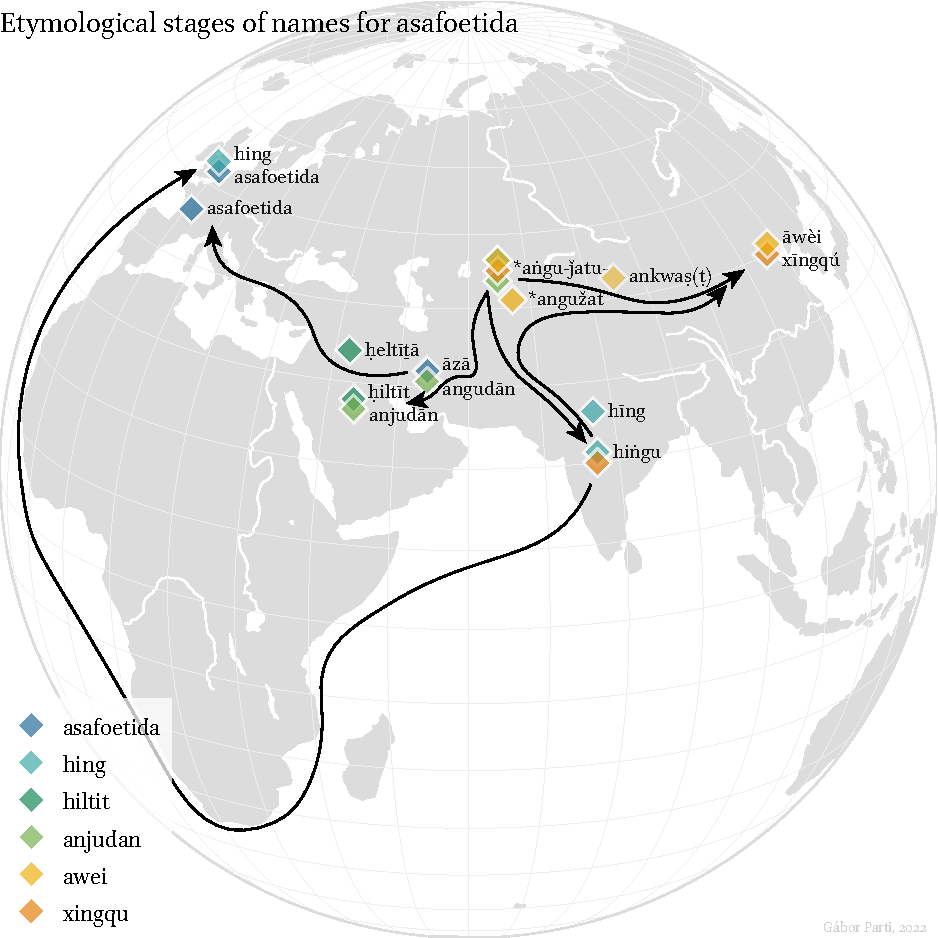
\includegraphics[width=\textwidth]{imgs/plots/diffusion_asafoetida_edited.pdf}
    \caption{Etymological stages in the progression of prototypical names of asafoetida.}
    \label{fig:cardamom_stages}
\end{figure}






% EE:
% asafoetida 
% resinous gum with a strong smell. XIV. — medL., lit. ‘stinking asa’, i.e. asa (usu. derived from a Persian azā mastic, but this word is of doubtful authenticity), fœtida, fem. of fœtidus FETID.

% OE:
% asafoetida (n.)
% alternative spelling of asafetida (q.v.); also see oe.
% asafetida (n.)
% "pungent sap from the roots of several plants native to Persia and Afghanistan," used as a drug, late 14c., from Medieval Latin asa (Latinized from Persian aza "mastic") + foetida, fem. of foetidus "stinking" (see fetid).

% MW:
% Middle English asafetida, from Medieval Latin asafoetida, from asa gum (of Iranian origin; akin to Persian azā mastic) + Latin foetida, feminine of foetidus fetid
% First Known Use: 14th century

% AH:
% [Middle English, from Medieval Latin asafētida : asa, gum (from Persian azā, mastic) + Latin foetida, feminine of foetidus, stinking; see FETID.]

% WK:
% Late Middle English, from Medieval Latin asafoetida, from Persian ازا / آزا (azâ, âzâ, “mastic”) + Latin foetida, feminine of foetidus (“bad-smelling”). 


% Synonyms: asant, hing, devil's dung

% MW:
% Hindi hī̃g, from Sanskrit hiṅgu

% AH:
% [Hindi, hīṁg, from Prakrit hiṁgu-, from Sanskrit hiṅgu, perhaps of Iranian origin; akin to Persian angu- in angužad, asafetida (angu- + žad, gum, tears of sap).]

% WK:
% From Hindi हींग (hīṅg). 





% \clearpage \section{Black Pepper}
\label{sec:pepper}

\begin{spice}\label{spice:pepper}
\textsc{Pepper} \hfill \href{https://powo.science.kew.org/taxon/682369-1}{POWO} \\
\textbf{English:} \textit{pepper}; \textit{black pepper}. 
\textbf{Arabic:} {\arabicfont{فلفل}} \textit{filfil, fulful}. 
\textbf{Chinese:} {\tradchinesefont{胡椒}} \textit{hújiāo} [foreign-pepper]; 黑胡椒 \textit{hēihújiāo} [black-barbarian-pepper]. 
\textbf{Hungarian:} \textit{bors}; \textit{fekete bors} [black pepper].  \\
\noindent{\color{black}\rule[0.5ex]{\linewidth}{.5pt}}
\begin{tabular}{@{}p{0.25\linewidth}@{}p{0.75\linewidth}@{}}
Plant species: & \taxonn{Piper nigrum}{L.} \\
Family: & \textit{Piperaceae} \\
Plant part used: & fruit \\
Region of origin: & Malabar coast (South India) \\
Cultivated in: & Vietnam; Brazil; Indonesia; India; Sri Lanka; etc. \\
Color: & black; white; green \\
\end{tabular}
\end{spice}

% \begin{figure}[!ht]
% 	\vspace{-4ex}
% 	\centering
% 	\subfloat{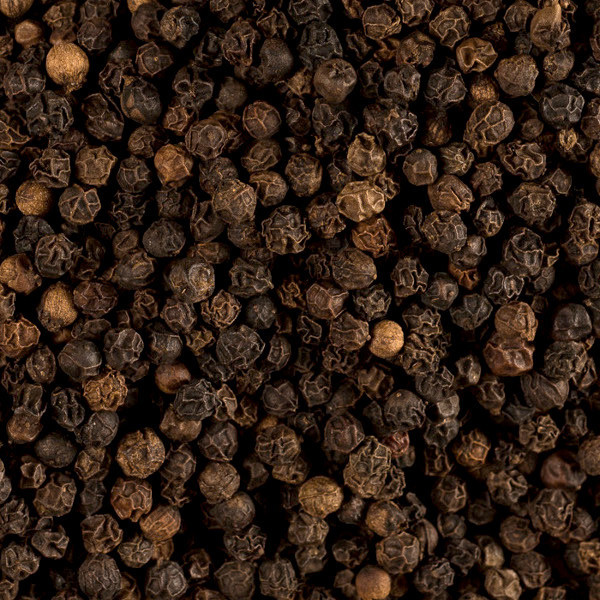
\includegraphics[width=0.3\linewidth]{imgs/spices/pepper-black-2.jpg}}
% 	\hfill
% 	\subfloat{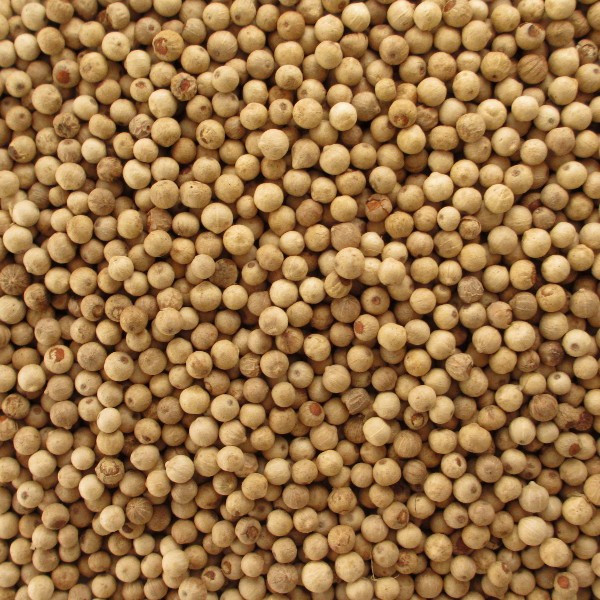
\includegraphics[width=0.3\linewidth]{imgs/spices/pepper-white-penja-2.jpg}}
% 	\hfill
% 	\subfloat{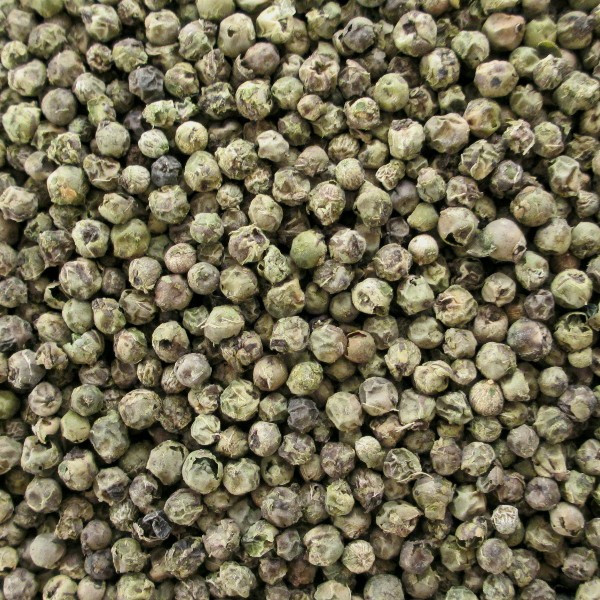
\includegraphics[width=0.3\linewidth]{imgs/spices/pepper-green-1.jpg}}
% 	\caption[Black, white, and green pepper.]{Black pepper from the Malabar coast in India, white pepper from the Penja Valley in Cameroon, and green peppercorns. \taxon{Piper nigrum}. Credits: Aromatiques.}
% 	\label{fig:pepper_imgs}
% \end{figure}

% DESCRIPTION:
Black pepper is the dried fruit (drupe)\footnote{Botanical term: A drupe refers to a type of fleshy fruit with thin skin and a single, central pit containing the seed, also known as a ``stone-fruit'' (e.g.: plum, cherry, peach, nutmeg, olive, mango). It is a term used to denote the contrast to a botanical ``berry'', which contains many seeds (e.g.: blueberry, grape).} of the species \taxon{Piper nigrum}. Pepper fruits are often called peppercorns, and they come in black, white, green, and even red. However, black pepper\index{pepper!black}, white pepper\index{pepper!white}, green\index{pepper!green} and ``true'' red peppercorns\index{pepper!red} are not different varieties, they are the fruits of the same plant. Their difference merely lies in the harvesting and drying process. All of them have a unique, pungent taste and a fresh, spicy aroma that they release when being crushed or ground. 

% INTRO:
Black pepper\index{pepper|textbf}\index{pepper!black} is the most important, most popular, and most consumed spice in the world \autocite[721]{mabberley_mabberleys_2017}. Valued for its pungency and flavor, pepper has been used since ancient times in traditional medicine and gastronomy from East to West, and it is the most influential spice that shaped human history. It is found and used virtually everywhere around the globe \autocite[253]{hill_contemporary_2004}, and most of us are familiar with the biting sensation it causes on the tongue and in the nose. Black pepper was one of the first aromatic substances used medicinally in India, and one of the first products of global commerce to be traded, alongside long pepper, and ginger. It was transplanted to other tropical regions of Asia early on, and cultivated extensively. Black pepper's early diffusion is remarkably interesting, it is the prototype spice for many of us. Also referred to simply as \textit{pepper} from here on, it was among the first oriental spices to reach the Occident \pvolcite[]{1}[86]{peter_handbook_2012}. Pepper was known to the ancient Egyptians, Greeks, and Romans in the West, and have changed medieval Europe. It was even used as currency in small amounts. Today it accounts for more than a third of all spices traded in the world, making it the most traded spice as well \autocite{ravindran_piper_2017}. Its importance is well demonstrated by the many books and monographs about its history \autocite[see][]{shaffer_pepper_2013,wernick_pepper_2014}, agronomy \autocite[see][]{ravindran_black_2000,nair_geography_2020}, and appeal \autocite[see][]{de_kerros_pepper_2016,barth_pepper_2019}.

% EXTRAS
Interestingly, black pepper is the only spice to be traded on the stock market as a commodity, the International Pepper Exchange was established in 1997 in Kochi, India. One result of this is cargo containers of black pepper sitting in warehouses waiting to change hands, leading to a loss in nutritional value and flavour and thus an unnecessary underwhelming experience for future consumers \autocite{madagascar_spices_company_madagascar_2022}. Spice merchants often urge serious customers to buy directly from the producer cutting the middlemen, citing the above inconvenience of product waiting in transit and retail.

\subsubsection{Uses}

% USES
% It was used
% for different purposes by different people in the past, and continue to be so currently and
% will remain so in future as well. For the civilized western people it is a spice, an essential
% additive to their food; for the ancient Egyptians it was an ingredient in the embalming
% mixture; for the ancient Aryans it was a valuable drug, and now for the common Indians
% pepper is a spice as well as a medicine, a sure cure for cold and fever and a component of
% many traditional Ayurvedic drugs. Stories richly coloured with imagination were carried
% by ancient sailors to distant places and its fame reached both Western and Eastern lands.
% The white pepper of commerce is also a product from the same pepper plant,
% produced by removing the pericarp (fruit wall) from ripe pepper fruits, which give the
% buff coloured seeds—the white pepper. White pepper is preferred in certain countries
% and also by the elite users because it gives a uniformly dull white powder; while black
% % pepper powder has the black component resulting from the powdered black pericarp.
% White pepper is traditionally prepared by steeping ripe fruits in water for a few days,
% rubbing to remove the pericarp; washing and drying. Indonesia is the major producer \autocite[1]{ravindran}

Black pepper had and has various uses in multiple areas. Nowadays, we mainly consider its importance in the culinary arts --- from seasoning food in the kitchen to the dining table --- but it is extensively used in the food industry as well for flavouring and preserving processed foods \pvolcite[]{1}[86]{peter_handbook_2012}.
% CULINARY USES:
Often called the ``king of spices'', black pepper is so ubiquitous and well known in cooking that it is essentially pointless to list cuisines and dishes that feature it. It is present in practically all savoury dishes, sauces, marinades, and pickles. It is used whole, crushed, or ground, and its role in Western gastronomy is well marked by the fact that virtually all restaurant table host a pair of salt and pepper mills or shakers. On the other hand, white pepper is a key ingredient in French and Chinese cuisine, where it is much more popular than black pepper, while green pepper is popular in Thai and South Indian cooking. 
% SEE PETER FOR MORE CULINARY
% MEDICINE
But besides just a seasoning, pepper also has roles in perfumery and beauty care, not to mention its use as a home remedy \autocite[467]{ravindran_black_2000}. In fact, as it is true for most spices, pepper in the past was considered primarily a medicine. Black pepper is well known in the traditional herbal systems, whether Ancient Greek, Ayurvedic, or Traditional Chinese Medicine, as well as contemporary pharmacology and phytotherapy (a modern name for chemistry-assisted herbalism). Reviews and updates on the research of \textit{Piper nigrum}, its active components, and their effects on human physiology are being published at a steady pace \autocite[see][]{srinivasan_black_2007, butt_black_2013, meghwal_piper_2013, haq_piperine_2021}. Recent scientific research shows that piperine displays numerous pharmacological effects, such as antimicrobial and antioxidant \autocite{haq_piperine_2021}. It is therefore not surprising that health benefits of black pepper have been recorded in pharmacopoeias since ancient times, and that it has been used for the treating of various illnesses: ranging from stomach pains and digestive problems to fever, cold, and even food poisoning \autocite[2952]{quattrocchi_crc_2014}.

% OPERATIVE
\begin{note}
Throughout this dissertation --- unless stated otherwise --- the term \textit{pepper} alone always denotes the pepper(s) of \taxon{Piper nigrum}, of the genus \textit{Piper}, from the pepper family (\taxon{Piperaceae}) or , originating in India (i.e. black pepper, white pepper, etc.). This is to make an arbitrary distinction with the various kinds of hot chile, or chili peppers of the genus \textit{Capsicum} in the nightshade family (\textit{Solanaceae}), native to the Americas. A partial objective of this dissertation is to untangle the messy nomenclature around these plant and spice names, which is evident if we take into account all the different items we can refer to with the words \textit{pepper} in English, \textit{jiāo} in Chinese, and \textit{filfil} in Arabic; a situation true to many other languages as well. 
% This notion is explored in more detail in \cref{sec:conundrum}
\end{note}

\subsubsection{False peppers}

There are other aromatic, spice yielding plants (other kinds of peppers, if you like) in the \textit{Piperaceae} family, constituting to different species, such as cubebs, tailed peppers, or Java peppers (\taxon{Piper cubeba}), (Indian) long peppers (\taxon{P. longum; P. retrofactum}), ``piper chilies'' (\taxon{P. chaba}), Ashanti/Benin pepper (\textit{P. guineense}), etc., and they will be referred to using these common names throughout. Cubeb, and  long pepper especially, were more common in ancient times but virtually disappeared from the global spice trade in the modern age. Other, less common spices unrelated to the \textit{Piper} genus, such as pink peppercorns from South America (\textit{Schinus molle; S. terebinthifolia}), Sichuan peppers from East Asia (\textit{Zanthoxylum spp.}), and alligator peppers (\taxon{Aframomum danielli}) from Africa are sometimes referred to as ``false peppers''. These will always be referred to with their usual full vernacular names to avoid confusion.
% (America pepper: chili) and peppercorn more to true pepper) explain in the pepper conundrum section.

Do other peppers at the end of this






\subsection{The Botany of Black Pepper} 

% ORIGIN:
Pepper is native to the Malabar region in South India where the Western Ghats, a mountain range parallel to the coastline, traps the monsoon rains. This results in the most humid region in India, making it one of the plant biodiversity hot-spots on Earth \autocite[1]{ravindran_black_2000}. Often called the ``king of spices'', pepper originates here in the evergreen tropical forests of Kerala, which is the origin and centre of plant diversity for the ``queen of spices'' as well: cardamom \autocite[1]{ravindran_black_2000}.
Wild populations of pepper and closely related species grow in the moist, shady forests, up to 1200\,m above sea level \autocite{ravindran_piper_2017}. Pepper is cultivated for thousands of years in these areas, and once South India was the only place that produced it. Due to the human desire for this valuable spice, the crop was slowly transplanted from here to other tropical zones, mainly in the Asia-Pacific: Sri Lanka, Malaysia, Indonesia; but also to the West as far as Madagascar and Brazil. Today it is cultivated in 26 countries \autocite{ravindran_black_2000}. The top five producers in 2020 were Vietnam, Brazil, Indonesia, India, and Sri Lanka.\footnote{In order of production quantity, from highest to lowest. All production data is from FAOSTAT (Food and agriculture data of the Statistics Division, Food and Agriculture Organization of the United Nations): \url{https://www.fao.org/faostat/en/\#home}; license: CC BY-NC-SA 3.0 IGO.}
% THE PLANT:
Pepper grows on a perennial vine, blooming a cluster of small flowers on hanging spikes that bring young, round fruits that are first green, turning to bright red as they ripen; resembling berries. Pepper plants in their native habitats spread on the forest floor, or climb over rocks, shrubs, and trees. Pepper prefers the hot tropics with high humidity, and optimal temperatures of around 20-30°C. Open cultivation is possible in places where rainfall is well distributed (e.g.: Thailand, Vietnam, Malaysia), whereas in India shade is required because of the 6 months of drought between monsoon seasons \autocite{ravindran_piper_2017}. Wild pepper species are dioecious\footnote{Bot.: the male and female reproductive organs are found in separate individuals.}, having male and female individuals, while the domesticated pepper populations became monoecious:\footnote{Bot.: having both the male and female reproductive organs in the same individual; hermaphrodite.} one plant is both male and female. This is probably due to thousands of years of selective multiplication and it leads to greater quantities in production: bisexual flowers mean high fruit yields \autocite[38]{ravindran_black_2000}.
% CULTIVATION:
Pepper lianes are propagated from cuttings, and being climbers, they are usually grown around trees for live support, or with the use artificial poles \autocite[216]{van_wyk_culinary_2014}. 

% HARVESTING:
When it comes to harvesting, the techniques are different depending on the intended end product. In the case of black pepper, the near-ripe (still green) fruits are hand-picked and sun-dried in the course of several days up to two weeks. Oxidization leads to the darkening of the pericarp\footnote{Bot.: In fruit anatomy, pericarp is the collective name for the outer layers around the seed of a fleshy fruit or drupe: the endocarp (innermost covering of the seed; the pit), the mesocarp (flesh), and the exocarp (skin).} (the outside skin and flesh of the fruit) to a hue ranging from deep brown to jet black, while also attaining the signature wrinkles and dimples \autocite[254]{hill_contemporary_2004}. The drying process can be sped up by boiling the pepper fruits in hot water for a short time. Chemical changes induced by the heat hasten the subsequent oxidization process, which causes the outer layer to gradually shrivel and blacken while getting dried \autocite[216]{van_wyk_culinary_2014}. White pepper is obtained by letting moisture and micro-organism dissolve the cellular tissue of the fully ripe red fruits, basically letting them rot in a technique called retting\footnote{}. The fruits' decomposed skin and flesh are easily removed by hand or machine after soaking and gentle washing, and the remaining pale seed is then dried on the sun, or bleached \autocite[216]{van_wyk_culinary_2014}. Green peppercorns are a result of traditional pickling, or in modern times rapid freeze-drying of the unripe fruits as a way to prevent fermentation. This process results in a product with a light weight and seemingly higher price. Occasionally the ripe, red fruits are sold as well to be used fresh, but the ``true'' red peppercorns -- as \textcite{hill_contemporary_2004} calls them -- are rare and mostly found in producing areas: they loose their vigour within days of harvest and so must be used fresh unless preserved in vinegar or brine. As it is a hallmark of spices, the two varieties that are dried (black pepper and white pepper) are much more known worldwide, their dry quality allows them to be transported on longer journeys. If we think of white pepper as de facto decorticated black pepper, we would rightly guess that the flavour of white pepper is weaker than black pepper, as the outer peel of black pepper contains much of the spicy compounds responsible for the heat. Green peppercorns have an even milder taste and a much shorter shelf-life.
%CULTIVARS
Indigenous to the Malabar coast, a well known and popular variant is the Malabar pepper or Malabar black, a commodity sought-after by traders since Roman times \autocite{de_romanis_indo-roman_2020}. Another famous name on the market is the Tellicherry black, which according to spice traders is not a regional designation, but rather a requirement of size. If a peppercorn is larger than 4.25 mm pinhead, it is classified as Tellicherry \autocite{eirinberg_tellicherry_2021}. Other famous and/or protected pepper variants with Geographical Indication (GI) certificates are Kampot pepper from Cambodia, the Muntok white and Sarawak white from Indonesia and Malaysia respectively, and the Penja pepper from Cameroon. A relatively recent publication by pepper grower and merchant \textcite{de_kerros_pepper_2016} accompanied by remarkable photographs aims to present all the dozens of pepper varieties around the world that are available to those with an adventurous taste.
% FLAVOUR COMPOUNDS:
Pepper owes its punch to the alkaloid piperine, while the wrinkly pericarp supplies the complex spicy aroma and flavour thanks to a high number of chemical compounds in the form of volatile oils \autocite[467]{ravindran_black_2000}. The most powerful one of which is rotundone, a highly potent compound also found in Shiraz wines \autocite{wood_wine_2008}. For more on details on the botany, chemistry, cultivation, agronomy, and other aspects of black pepper, please refer to \textcite{ravindran_black_2000, nair_agronomy_2011, parthasarathy_chemistry_2008}.



% HISTORY:
\subsection{The History of Black Pepper}

The history of pepper accompanies the history of mankind from the earliest times of contact and exchange between civilizations. The story of pepper is global and must travel to Ancient Egypt to begin. According to a popular anecdote in books and articles about pepper, peppercorns were used in the embalming process of mummies \autocite{ravindran_black_2000}, and they were found in the nostrils of Ramses II \autocite[168]{turner_spice_2004}. I have read this on many occasions, and I have spend way too much time to find out if this is true or not. In short, I there is no definitive answer, but that the alleged peppercorns were only ``seen'' through X-ray, and that the original reports are dubious at best, as reported by \textcite[206]{bucaille_mummies_1990}. Ramses II died in 1213 \BC{}, and even if these specific are problematic, it is said that peppercorns and cinnamon were imported ``from Southeast Asia and the East Indies'' and thus available to wealthy citizens of Egypt as early as New Kingdom era (\nth{16} c. \BC{}--\nth{11} c. \BC{}) \autocite[394]{salima_diet_2005}.

Pāṇini, the famous Sanskrit grammarian (ca. 4--\nth{6} c. \BC{}) recorded the use of pepper in spiced wine, and pepper appears in early Indian medical texts of Suśruta as well \autocite{ravindran_black_2000}. In the \nth{4} century, Theophrastus recorded and described both black pepper and long pepper, and by the \nth{1} century \AD{} its source was accurately describe by Pliny the Elder; stating that black pepper is from south, long pepper is from north India. Rome conquered Egypt in 30 \BC{}, and with that the pepper trade as well, which was a key enterprise in Rome's later financial success. From here onwards, the history of pepper within the Indo-Roman trade is well studied and documented, for further details please see \textcite{sidebotham_berenike_2011,de_romanis_indo-roman_2020,miller_spice_1969}. 

% Peppercorn in fist century as far as Germany (Czarra)

During the late Middle Ages, pepper also brought great riches to Europe, the former wealth of Venice was due to its trade. After the crusades, European sea powers tried to get ahold on the monopoly of the spice trade, and Vasco de Gama's landing near Calicut in 1498 in the Venetian, Portuguese, Spanish, Dutch, and English vied with each other for centuries up to the modern era. Pepper reached Southeast Asia probably during the t The story of pepper is very well explored in the Age of Exploration as well, there is no need for me to delve into it deeper. I recommend \textcite{shaffer_pepper_2013,turner_spice_2004,dalby_dangerous_2000} for those interested.

% A Chinese envoy visited the Malabar coast in search of pepper. 4th c. BC? Who

% TIMELINE IN RAVINDRAN
% Originally black pepper was a forest produce
% Black pepper was essentially a forest produce in the past, people collected it from
% forests, where it abounded. The collected pepper was brought to local markets for
% retail trade with Arab merchants. Domestication of pepper appears to be a much later
% event. There is, only speculative evidence as to when pepper was introduced to other
% countries as a domesticated crop. Colonists from India are believed to have introduced
% pepper cultivation to Indonesia about 100 B.C. (Rosengarten 1973). Many such
% introductions surely might have taken place subsequently also. The landmarks in the
% colourful history of pepper are given below. Ravindran 2000 

% \autocite{pegolotti_pratica_1936}

% Wyk:
% Pepper featured prominently in the
% ancient world and was a source of fabulous wealth
% during the medieval and colonial spice trade. The
% Dutch and Afrikaans expression “peperduur”
% reflects the high price it once had. Pepper provided
% the pungency (“pep”) of Indian food until it was
% partially replaced by chilli peppers from the New
% World. It nevertheless remains the most important
% and popular of all spices in terms of overall value
% and trade volume.

% Black pepper is the most important and widely used spice. Black pepper (hereafter mentioned simply as pepper) is valued for its characteristic pungency and flavour. It has been used extensively from ancient times as a spice and condiment in a variety of food preparations. Pepper is famous as a traditional medicine; it is also famous as a home remedy. Globally, pepper accounts for 34\% of the total spices traded. In all countries pepper is used for flavouring food and for preserving processed foods. Pepper played a very significant role in shaping the history of mankind. It was the first oriental spice to reach the Western world. The European nations vied with each other to get the monopoly over the spice trade and hegemony over the spice-producing countries of the East that eventually led to the discovery of a sea route to India by Vasco da Gama. This event changed the history of the world radically in the centuries that followed. ENCYC

% Among the spices, black pepper is the king. It is the most important, the most
% popular and the most widely used spice in the world. It has extensive culinary uses
% for flavoring and preserving processed foods and is also important medicinally. Of
% the total spices traded internationally, pepper accounts for about 34 % (throughout
% this chapter, pepper is used to mean black pepper, unless otherwise stated). South
% West India, particularly the Western Ghats regions of the South India, is the centre
% of origin of this important spice. Black pepper was the fi rst oriental spice to be
% introduced into the Western world, and it was well known among the Romans and
% Greeks. In the Middle Ages, pepper, assumed great importance in Europe. Its use
% resulted in revolutionary changes in western cooking. For a comprehensive treatment
% of black pepper, the reader may consult Ravindran (2000a) and Ravindran
% et al. (2006). Bezerra et al. recently (2009) summarized the various aspects of black

\subsection{The Names of Black Pepper}

\subsubsection{English}

\begin{etymology}\label{ety:pepper}
English \textit{pepper}
<\textss{?} West Germanic* \textit{*pipor} `id.'
< Latin \textit{piper} `black pepper, long pepper'
< Ancient Greek {πέπερι} \textit{péperi} `id.'
< Middle Indo-Aryan* {पिप्परी } \textit{pipparī} `long pepper'
< Sanskrit {पिप्पलि } \textit{pippali} `long pepper \textit{Piper longum} (plant and berry); a berry'\footnote{\textcite{oed; med; bosworth_anglo-saxon_2014}; \textcite{oe}; \textcite{lewis_latin_1879}; \textcite{liddell_greek-english_1940}; \textcite[599]{sheth_paia-sadda-mahannavo_1923}; \textcite[626]{monier-williams_sanskrit-english_1899}}
\end{etymology}

The word \textit{pepper} arrived to modern English via Middle English \textit{peper} and Old English \textit{pipor, piper}, from an early, Proto-West Germanic borrowing of Latin \textit{piper}.\footcite[pepper]{oed} The Latin word comes from Greek \gr{πέπερι} \textit{péperi}, a word ``of oriental origin''\footcite[pepper]{hoad_concise_2003} or ``Indic origin''.\footcite[pepper]{ahd} The source is most probably from a Middle Indo-Aryan language, akin to Prakrit \textit{pipparī}\footcite[599]{sheth_paia-sadda-mahannavo_1923}, probably via Pahlavi (Middle Persian)\footcite[pepper]{oe}, ultimately from Sanskrit \textit{pippali} or \textit{pippalī}.\footcite[628 \link{https://www.sanskrit-lexicon.uni-koeln.de/scans/MWScan/2014/web/webtc/servepdf.php?page=0628}]{monier-williams_sanskrit-english_1899}

As for the meaning, we know that in Latin the word \textit{piper} was used for both black pepper and long pepper, and this is true for the Greek word as well. As long pepper gradually disappeared and was completely replaced by black pepper in the Middle Ages, so vaned the that sense of the word. The original word's meaning however was exclusively long pepper, \textit{pippali} did not refer to black pepper. In \textcite{monier-williams_sanskrit-english_1899}, \textit{pippali} is `long pepper', while \textit{pippalī} refers to `a berry; Piper longum (both plant and berry)'. The Sanskrit word for `black pepper' was \sa{मरिच} \textit{marica}\footcite[790]{monier-williams_sanskrit-english_1899}, attested in the \gls{Sushruta}, the foundational text of \gls{Ayurveda}. Hindi-Urdu \sa{मिर्च}/\fa{مرچ} \textit{mirch} is the most obvious descendant of the Sanskrit word, and it is similar in meanings to the word \textit{pepper} in English today: by itself it rather refers to chili, while with a distinguishing word, it refers to black pepper (i.e. \textit{kālī mirc} [black pepper]). The use of both black and long pepper in India can be dated to ancient times, as Ayurvedic texts compiled in Sanskrit, such as the \gls{Sushruta} testify. Together with ginger (\textit{śṛṅgavera} in Sanskrit), these three spices are a base combination in traditional Indian medicine, the name for which is \sa{त्रिकटु} \textit{trikaṭu} `three spices'.

The ancestors of English speakers adopted the word during the Anglo-Saxon period, before they arrived to England, and so its cognates are found in other West Germanic languages as well.\footcite[pepper]{cresswell_oxford_2021} 

% Cognates:  Old Saxon \textit{pipari}, \textit{pepar} (Dutch \textit{peper}, Scots pepar), Old High German \textit{pfeffar} (German \textit{Pfeffer}), Old Norse \textit{piparr} (Danish \textit{peber}, Swedish \textit{peppar}, Icelandic \textit{pipar}).

According to \textcite[695]{mabberley_mabberleys_2017}, the following common names refer to the species \textit{Piper nigrum}: pepper, black pepper, Madagascar pepper, and white pepper. Except the green peppercorns mentioned above, other spices, such as the Sichuan peppers from China, pink peppercorns from Brazil, and Guinea peppers (\textit{Aframomum melegueta}) from tropical West Africa are different, often botanically unrelated species. Only connected by their names and similar uses, looks, or flavour profiles.


% Leaves of P. sarmentosum are the cha plu of Thai cuisine and those of P. auritum the hoja santa of Mexican cuisine. Plus Piper betle = betel? no.

% \begin{table}[!ht]
\centering
\begin{tabularx}{\textwidth}{@{}l>{\itshape \small}lL>{\small}l@{}}
\toprule
\textbf{\#} & \multicolumn{1}{l}{\textbf{Species}} & \multicolumn{1}{l}{\textbf{Name}} & \multicolumn{1}{l}{\textbf{Source}} \\
\midrule
1	& Piper nigrum	& black pepper	& \textcite{van_wyk_culinary_2014} \\
2	& Piper nigrum	& green pepper	& \textcite{oed} \\
\textbf{3}	& \textbf{Piper nigrum}	& \textbf{pepper}	& \textbf{\textcite{van_wyk_culinary_2014}} \\
4	& Piper nigrum	& peppercorn	& \textcite{oed} \\
5	& Piper nigrum	& white pepper	& \textcite{oed} \\
\bottomrule
\end{tabularx}
\caption{Various names for pepper in English.}
\label{table:names_pepper_en}
\end{table}



% \subsubsection{Arabic}

% \begin{etymology}\label{ety:fulful}
Arabic {فلفل} \textit{filfil, fulful} `pepper'
< Persian {پلپل} \textit{pilpil} `id.'; cf. cognates Old Armenian \hy{պղպեղ} \textit{płpeł}, Old Georgian \ka{პილპილი} \textit{ṗilṗili}
<\textss{?} Middle Indo-Aryan \textit{?} `long pepper'
< Sanskrit {पिप्पलि } \textit{pippali} `long pepper \textit{Piper longum} (plant and berry); a berry'\footnote{\textcite[2434]{lane_arabic-english_1863}; \textcite{sq}}
\end{etymology}

% \begin{table}[!ht]
\centering
\begin{tabularx}{\textwidth}{@{}l>{\itshape \small}lr>{\itshape}lL>{\small}l@{}}
\toprule
\textbf{\#} & \multicolumn{1}{l}{\textbf{Species}} & \multicolumn{1}{l}{\textbf{Name}} & \multicolumn{1}{l}{\textbf{Tr.}} & \multicolumn{1}{l}{\textbf{Gloss}} & \multicolumn{1}{l}{\textbf{Source}} \\
\midrule
\textbf{1}	& \textbf{Piper nigrum}	& \textbf{فلفل}	& \textbf{fulful}	& \textbf{pepper}	& \textbf{\textcite{wehr_dictionary_1976}} \\
2	& Piper nigrum	& فلفل أبيض	& fulful abyaḍ	& white pepper	& \textcite{baalbaki_-mawrid_1995} \\
3	& Piper nigrum	& فلفل أسود	& fulful aswad	& black pepper	& \textcite{baalbaki_-mawrid_1995} \\
4	& Piper nigrum	& فلفلة	& fulfula	& peppercorn	& \textcite{wehr_dictionary_1976} \\
\bottomrule
\end{tabularx}
\caption{Various names for pepper in Arabic.}
\label{table:names_pepper_ar}
\end{table}



% \subsubsection{Chinese}

% \begin{etymology}\label{ety:hujiao}
\textbf{Mandarin Chinese} {胡椒} \textit{hú​jiāo} `black pepper' [barbarian-pepper], from 胡 \textit{hú​} `Western barbarians, steppe nomads' + 椒 \textit{jiāo} `pepper, spice' (\textit{jiāo} was the prototype spice in China, originally referring to the local ``Sichuan pepper'' which is now called 花椒 \textit{huājiāo} [flower-pepper]), [Northern and Southern] 420-445\footnote{\textcite{schuessler_abc_2007}}
\end{etymology}

% \begin{table}[!ht]
\centering
\begin{tabularx}{\textwidth}{@{}l>{\itshape \small}ll>{\itshape}lL>{\small}l@{}}
\toprule
\textbf{\#} & \multicolumn{1}{l}{\textbf{Species}} & \multicolumn{1}{l}{\textbf{Name}} & \multicolumn{1}{l}{\textbf{Tr.}} & \multicolumn{1}{l}{\textbf{Gloss}} & \multicolumn{1}{l}{\textbf{Source}} \\
\midrule
1	& Piper nigrum	& \tradchinesefont{白胡椒}	& báihújiāo	& white-barbarian-pepper	& \textcite{mdbg} \\
\textbf{2}	& \textbf{Piper nigrum}	& \textbf{\tradchinesefont{胡椒}}	& \textbf{hújiāo}	& \textbf{barbarian-pepper}	& \textbf{\textcite{hu_food_2005}} \\
3	& Piper nigrum	& \tradchinesefont{黑胡椒}	& hēihújiāo	& black-barbarian-pepper	& \textcite{mdbg} \\
4	& Piper nigrum	& \tradchinesefont{綠胡椒}	& lǜhújiāo	& green-barbarian-pepper	& \textcite{regency_spices_regency_2022} \\
5	& Piper nigrum	& \tradchinesefont{青胡椒}	& qīnghújiāo	& green-barbarian-pepper	& \textcite{regency_spices_regency_2022} \\
\bottomrule
\end{tabularx}
\caption{Various names for pepper in Chinese.}
\label{table:names_pepper_zh}
\end{table}



% \subsubsection{Summary}

% \begin{table}[!ht]
\centering
\begin{tabularx}{\textwidth}{@{}ll>{\itshape}lLl>{\small}l@{}}
\toprule
\textbf{\#} & \textbf{Language} & \multicolumn{1}{l}{\textbf{Term}} & \textbf{Gloss} & \textbf{Loan} & \multicolumn{1}{l}{\textbf{Source}} \\
\midrule
1	& English	& black pepper	& 	& maybe	& \textcite{oed} \\
2	& English	& pepper	& 	& yes	& \textcite{oed} \\
3	& English	& white pepper	& 	& maybe	& \textcite{oed} \\
\midrule
1	& Arabic	& fulful	& pepper	& yes	& \textcite{wehr_dictionary_1976} \\
2	& Arabic	& fulful abyaḍ	& white pepper	& no	& \textcite{baalbaki_-mawrid_1995} \\
3	& Arabic	& fulful aswad	& black pepper	& no	& \textcite{baalbaki_-mawrid_1995} \\
4	& Arabic	& fulfula	& peppercorn	& no	& \textcite{wehr_dictionary_1976} \\
\midrule
1	& Chinese	& báihújiāo	& white-barbarian-pepper	& no	& \textcite{mdbg} \\
2	& Chinese	& hújiāo	& barbarian-pepper	& no	& \textcite{defrancis_abc_2003} \\
3	& Chinese	& hēihújiāo	& black-barbarian-pepper	& no	& \textcite{mdbg} \\
\bottomrule
\end{tabularx}
\caption{Conventionalized names for pepper in English, Arabic, and Chinese, found in dictionaries.}
\label{table:names_pepper}
\end{table}










% \begin{figure}[!hbt]
%     \centering
%     \includegraphics[width=\linewidth]{imgs/pepper.pdf}
%     \caption{Etymology of the English word \textit{pepper}, and an illustration of its approximate route.}
%     \label{map:pepper_etymology}
% \end{figure}



% EE: The Concise Oxford Dictionary of English Etymology:
% OE. piper, -or = OS. pipari, pepar (Du. peper), OHG. pfeffar (G. pfeffer); WGmc. — L. piper — Gr. péperi, of oriental orig.; cf. Skr. pippalī́t berry, peppercorn.

% OE: 
% pepper (n.)
% "dried berries of the pepper plant," Middle English peper, from Old English pipor, from an early West Germanic borrowing of Latin piper "pepper," from Greek piperi, probably (via Persian) from Middle Indic pippari, from Sanskrit pippali "long pepper." The Latin word is the source of German Pfeffer, Italian pepe, French poivre, Old Church Slavonic pipru, Lithuanian pipiras, Old Irish piobhar, Welsh pybyr, etc.
% Application to fruits of the Capsicum family (unrelated, originally native of tropical America) is from 16c. To have pepper in the nose in Middle English was "to be supercilious or unapproachable."
% pepper (v.)
% "to sprinkle as with pepper," 1610s, from pepper (n.). Old English had gepipera. Meaning "to pelt with shot, etc.; hit with what pains or annoys" is from 1640s. Related: Peppered; peppering.

% MW:
% Middle English peper, from Old English pipor; akin to Old High German pfeffar pepper, Old Norse piparr; all from a prehistoric Germanic word borrowed from Latin piper pepper, from Greek peperi, probably from Sanskrit pippali long pepper
% First Known Use: before 12th century (sense 1a)

% AH:
% [Middle English peper, from Old English pipor, from Latin piper, long pepper, black pepper, from Greek peperi, of Indic origin; akin to Prakrit pipparī, long pepper, from Sanskrit pippalī, from pippalam, berry, fruit of the pipal tree, of unknown origin.]

% WK:
% From Middle English peper, piper, from Old English piper, from Proto-West Germanic *piper, from Latin piper, from an Indo-Aryan source; compare Sanskrit पिप्पलि (pippali, “long pepper”). The name was given to the capsicum fruit because of its unusual spicy taste, not unlike the European spice.

% Wo: The Oxford Dictionary of Word Origins:
% The Anglo-Saxons adopted the word for this highly prized spice before they invaded England, for it is found in other West Germanic languages. The word came via Latin from Greek peperi, from Sanskrit pippalī ‘berry, peppercorn’. 
%The phrase peppercorn rent is from the once-common practice of stipulating the payment of a peppercorn as a nominal rent. (true?)
% Cognate with Scots pepar, Saterland Frisian Pieper, West Frisian piper, Dutch peper, German Low German Peper, German Pfeffer, Danish peber, Swedish peppar, Icelandic pipar. Doublet of peepul. 



% The pepper conundrum:

% Before we delve into the chaos of \textit{pepper-linguistics}, we should make the botany and geography absolutely clear. There are essentially three major sources of edibles we can refer to as peppers: (1) \textit{Piper}, a pantropical\footnote{??} genus known for black and white pepper, long pepper, and cubeb pepper from South and South East Asia; (2) \textit{Capsicum}, the genus of both hot chile and mild bell pepper species and their numerous cultivars native to the Americas; and (3) \textit{Zanthoxylum}, a vast and cosmopolitan\footnote{??} genus of various species yielding Sichuan peppers favoured in East Asia. There are many more aromatic products denoted with the name \textit{pepper} in English, but for our task focusing on the above three genera is sufficient. Also, the majority of globally relevant ``peppers'' belong to these groups as well. Nevertheless, for a full paragraph of a detailed list of plants, please see \textcite[695]{mabberley_mabberleys_2017}.

% pepper Piper nigrum; African p. Xylopia aethiopica; Ashanti or Benin p. P. guineense; bell p. Capsicum annuum Grossum Group; p.berry Drimys spp.; betel p. P. betle; bird p. C. a.var.glabriusculum; black p. P. nigrum; bush p. Clethra alnifolia; cayenne p. Capsicum annuum Longum Group; cherry p. C. a. Cerasiforme Group; chilli p. C. a.Longum Group; Chinese p. Zanthoxylum simulans; cone p. C. a. Conoides Group; p.corns, pink or red Schinus terebinthifolius; Ethiopian p. X. aethiopica; green p. C. a. Grossum Group; Guinea p. Aframomum melegueta, X. aethiopica; Indian long p. P. longum; Jamaican p. Pimenta dioica; Japanese p. Z. piperitum; Java p. Piper cubeba; Kawa p. P. methysticum; long p. P. longum; Madagascar p. P. nigrum; malagueta or melegueta p. A. melegueta; negro p. X. aethiopica; red or sweet p. C. a. Grossum Group; Saturday-night p. Euphorbia helioscopia; Sichuan p. Z. simulans; p. tree S. molle, Kirkia wilmsii, P. excelsum; wall p. Sedum acre; water p. Persicaria hydropiper; W African black p. Piper clusii; white p. P. nigrum

% Pepper in English

% ...


The confusion of the two kinds of pepper -- most notably of black pepper and chile pepper in English -- is also present in Chinese, as well Arabic. Whether in culinary or medicinal spice terminology, or just in vernacular names in daily conversation, the curse of ``one word for all peppers'' is present in many languages.

\textit{Jiao} `pepper' in Chinese

In Chinese, the word for `pepper' is \textit{jiao}. And just like in English, \textit{jiao} now can refer to all the three major sources of pepper. So which pepper is it? \st{Who is the O.G. of peppers?}. It would be safe to assume that \textit{jiao} originally referred to indigenous Chinese peppers of various \textit{Zanthoxylum} species, or Sichuan peppers as we today call them. We can find instances of Classical Chinese texts featuring the pepper plant, \textit{jiao} and it's branches appear in a poem from the \textit{Book of Poetry}:

% \poemtitle{Mathematics}
\settowidth{\versewidth}{The clusters of the pepper plant,}
\begin{verse}[\versewidth]
椒聊之實、蕃衍盈升。\\
彼其之子、碩大無朋。\\
椒聊且、~~~~~~遠條且。\\!
The clusters of the pepper plant,\\
Large and luxuriant, would fill a pint.\\
That hero there\\
Is large and peerless.\\
O the pepper plant!\\
How its shoots extend!\\
\end{verse}
\attrib{Translated by James Legge, \\
from the \textit{Shijing}, \\
c. 8--\nth{11} century \BC.}

% Pre-Qin and Han -> Ancient Classics -> Book of Poetry -> Lessons from the states -> Odes Of Tang -> Jiao Liao

% Transl. James Legge
% https://ctext.org/book-of-poetry/jiao-liao?searchu=%E6%A4%92%E8%81%8A%E4%B9%8B%E5%AF%A6%E3%80%81%E8%95%83%E8%A1%8D%E7%9B%88%E5%8D%87%E3%80%82&searchmode=showall#result
% \url{https://en.wikipedia.org/wiki/Classic_of_Poetry}

% Our assumption will only strengthen if we search the word history of black pepper, a native of India. It first appears in
% https://ctext.org/pre-qin-and-han?searchu=%E8%83%A1%E6%A4%92

% Pre-Qin and Han


% The first occurrence of \textit{hujiao}

% The origin of hujiao `black pepper' in Chinese






% \begin{figure}
% \label{fig:pepper}
% \begin{forest}
% for tree={grow'=0,calign=center,font=\footnotesize, s sep=1,inner sep=1,outer sep=1},
% forked edges,
% [Sanskrit\\pippali
%     [Ardhamagadhi Prakrit\\pipparī [Awadhi\\pīpri]]
%     [Gandhari [Middle Iranian\\\textrightarrow [Persian\\pelpel [Arabic\\\textrightarrow filfil [Persian\\\textrightarrow felfel]] [(Arabic)\\\textrightarrow falāfil] [Baluchi\\\textrightarrow pilpil] [Hebrew\\\textrightarrow pilpel] [Swahili\\\textrightarrow pilipili] ] [Old Armenian\\\textrightarrow płpeł [Armenian\\\textrightarrow płpeł]] [Old Georgian\\\textrightarrow ṗilṗili [Georgian\\ṗilṗili]] ]]
%     [Pali\\pipphalī]
%     [Magadhi Prakrit [Assamese\\pipoli] [Bengali\\pipul] [Bhojpuri\\pīpri]]
%     [Maharastri Prakrit [Old Marathi\\piṃpaḷī [Marathi\\pimpḷī]] [Kannada\\\textrightarrow hippali]]
%     [Sauraseni\\Prakrit [Nepali\\piplā] [Gujarati\\pīpar] [Hindustani [Hindi\\pīpal; pīpar] [Urdu\\pīpal] [(English)\\\textrightarrow peepul]] [Punjabi\\pippalī] [Ancient Greek\\\textrightarrow péperi* [Greek\\pipéri [Ottoman\\Turkish\\biber [Turkish\\biber [Armenian\\bibar] [Azerbaijani\\bibər] [Crimean Tatar\\biber] [Macedonian\\biber] [Serbo-Croatian\\biber]]] [Aromanian\\piper]] [Latin\\\textrightarrow piper [Basque\\\textrightarrow piperra] [Middle Irish\\pipur [Irish\\piobar] [Manx\\pibbyr] [Scottish Gaelic\\peabar; piobar] [Old Norse\\piparr [Icelandic\\pipar] [Faroese\\pipar] [Norwegian\\pepar] [Swedish\\peparr [Finnish\\\textrightarrow pippuri [Northern Saami\\bihppor]]]] ] [Dalmatian\\pepro] [Italian\\pepe] [Old French\\poivre [French\\poivre]] [Aragonese;\\Catalan;\\Occitan\\pebre]]]]
%     [Old Tamil\\\textrightarrow [Tamil\\tippili] [Malayalam\\\textrightarrow tippali]]
%     [Telugu\\\textrightarrow pippali]
%     [Thai\\\textrightarrow dii-bplii]
%     [Tibetan\\\textrightarrow pi pi ling]
%     [Middle Chinese\\\textrightarrow MC piɪt̚ bʉɐt̚ [Chinese\\bìbá [Japanese\\\textrightarrow hihatsu] [Korean\\\textrightarrow pilbal]]]
% ]
% \end{forest}
% \caption{Caption}
% \end{figure}





% \small{aguttam, akuttam, alar, alarkay, alarkaycceti, alarmancal,
% alivaliyanmani, amiram, anam, apanam, apayam,
% aricam, aricu, aricuvai, arisu, arittam, arunapakam, arutam,
% aruttakam, aruttam, aruttan, arutti, atittam, aucatikam,
% autatalakamilaku, ayilakikam, bikran, cakankam,
% canucam, canucam, canukam, carapantam, carumapantam,
% catalam, catalamilaku, cattu-molagoi, cavi, cavviyam, cavviyapalam,
% cavyam, celavikacceti, celaviyam, cevviyam,
% ceytakar, chocamirch, cirovikam, ciroviruttam, citamaricam,
% citamarucam, citamarucu, citamarukam, cullituvan,
% cunam, cuppiramaniyam, cur, dhanwantari, dharmapattana,
% dharmavarttana, dolo maricho, eddemunchi, eddemunci,
% fiffile-asvad, fifile-asvad, fifile-gird, filfil aswad, filfil-esiyah,
% filfil siah, filfile-gird, filfile-siyah, filfilgird, filful
% aswad, filfilsiya, filfiluswud, gol mirc, gol-mirch, golmirch,
% golmorich, gulmirch, habush, hapusha, impikam, impilam,
% irambivam, irampikam, irampilam, irampivam, itukam, itukamilaku,
% ivainakitam, ivanattam, jalook, jaluk, kaalimirch,
% kaalu menasu, kadu menasu, kali mirch, kalimirc, kalimirch,
% kalamiri, kalappakacceti, kalappakam, kali mirch, kalimirch,
% kalimirich, kalinai, kalinaikkollu, kalinaimilaku, kalinkam,
% kallinai, kami, kamicakam, kanakam, kanattai, kandanaguli,
% kankola, kantanakuli, kantankuli, kaphavirodhi,
% karam, karee menasu, kari, karikkay, karimenasu, karunelli,
% karutturupayan, karyam, katti, kattirican, katu, katuka, kay,
% kayam, kevakatiraviyam, kevalatiraviyam, kirantikantikam,
% kirusnam, kiruttinam, kola, kolai, kolagam, kolaka, kolakam,
% kolam, kolicam, kolikacceti, krishnam, krishnamushana,
% krsna, kuru-milagu, kuru-mulaka, kurumilagu, kurumilaku,
% kurumulagu, kurumulaka, kurumulaku, maarichamu, maciyam,
% maikkurotikam, maiyi, makaracitakaram, malaittirukkal,
% malaivacapancam, malaiyalam, malaiyali, malaiyaracan,
% malaiyavikam, maliyavikacceti, malaiyinmunivan, malina,
% marica, marica-valli, maricam, maricamu, maricha, maricham,
% marichamu, marichi, marichipatra, marici, marisam,
% mariyal, maruci, marukkam, matankan, meervaela, mellaghoo,
% menasina balli, menasinaballi, menasinakaalu, menasinakalu,
% menasu, mensukaai, milagu, milagu-valli, milaku,
% milakucceti, milakuvalli, mir vel, mirc, mirch, mirch siah,
% mire, mireem, miremu, miri, miricam, miricanam, mirici,
% mirim, miriyaalathige, miriyaalu, miriyal, miriyala-tige,
% miriyalakam, miriyalatige, miriyalu, miriyamu, miriyarkoti,
% miryala-tige, miryalatige, molago-codi, molagacodi, moloovookodi,
% mrishta, mulaku, mulaku koti, mulakukoti, mulatti,
% munchi, munci, muntan, mupparitam, mupparitamilaku,
% murialtiga, musanam, mutanam, nakarenu, nallamilaku,
% nalmilaku, nattumilaku, neriyal, nettakam, nettam, nitiyam,
% olle menasu, ollemenasinaballi, ollemenasu, ollimonasu,
% ooshnam, palini, paluk, paluka, parici, pattuvanestam, pavita,
% pavitam, pilpil, piramamaricam, piramaparicam, pittam,
% pokhlem-mirim, pulipacitam, repam, ruksha, sabe-ricke,
% safedmirch, sarvahita, savyamu, shakanga, shevium, shirovritta,
% shivika, shudha, shyama, siyah mirch, suvrtta, tarapattanam,
% tarmapattanam, tarumapittam, tattuvacam, tavalam,
% tavalamilaku, thinghmarcha, ticcanam, tikshna, tiksna,
% tiraipokki, tirankal, tirankalam, tirankam, tirankanal, tirkuta,
% titcanam, tuvinam, ucakam, ucanam, uciram, usakam, usana,
% usanaka, usanam, ushanam, utanam, uttanam, vacampu,
% vacankiyam, vacikam, vacitam, vallacam, vallicam, vallija,
% vallijam, vallikacceti, valliyam, vara, varishtha, vatamarukkinron,
% vatanacani, vellaiccatikam, vellaiccatikamilaku,
% vellaimilaku, vellaja, vellajam, vellija, venkakkiyam, venkakkiyamilaku,
% venmilaku, venticam, venticamilaku, venuja,
% venuka, venunam, villajam, virani, viruttapalam, viruttapam,
% volloymenasu, vrittaphala, wollemenasu, yavanappiriyam,
% yavanapriya, yavaneshtha, yeddemunci, zira siyah}
% \clearpage 
\section{Caraway}
\label{sec:caraway}

\begin{spice}\label{spice:caraway}
\textsc{Caraway} \hfill \href{https://powo.science.kew.org/taxon/839677-1}{POWO} \\
\textbf{English:} \textit{caraway}. 
\textbf{Arabic:} {\arabicfont{كراويا}} \textit{karāwiyā}. 
\textbf{Chinese:} {\tradchinesefont{葛縷子}} \textit{gě​lǚ​zi}. 
\textbf{Hungarian:} \textit{fűszerkömény } [spice-cumin].  \\
\noindent{\color{black}\rule[0.5ex]{\linewidth}{.5pt}}
\begin{tabular}{@{}p{0.25\linewidth}@{}p{0.75\linewidth}@{}}
Plant species: & \taxonn{Carum carvi}{L.} \\
Family: & \textit{Apiaceae/Umbelliferae} \\
Plant part used: & fruit \\
Region of origin: & Mediterranean; Eurasia \\
Cultivated in: & Denmark, Lebanon, The Netherlands, Poland \\
Color: & nan \\
\end{tabular}
\end{spice}

% \begin{figure}[!ht]
% 	\vspace{-4ex}
% 	\centering
% 	\subfloat[\centering a]{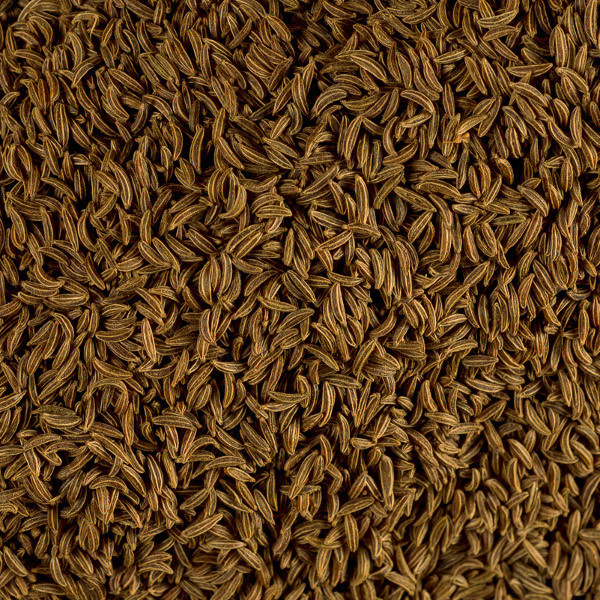
\includegraphics[width=0.3\linewidth]{imgs/spices/caraway-1.jpg}}
% 	\hfill
% 	\subfloat[\centering b]{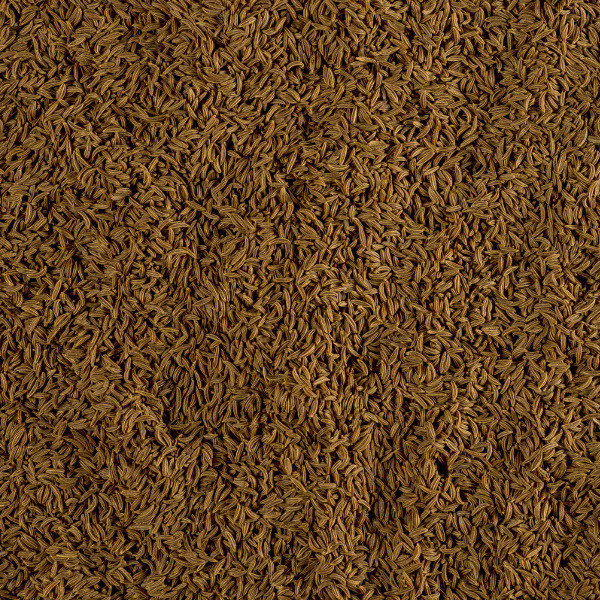
\includegraphics[width=0.3\linewidth]{imgs/spices/caraway-2.jpg}}
% % 	\hfill
% % 	\subfloat[\centering c]{\includegraphics[width=0.3\linewidth]{imgs/spices/caraway3.jpg}}
% 	\caption{Caraway \textit{Carum carvi}.}
% 	\label{fig:caraway_imgs}
% \end{figure}

\begin{wrapfigure}{R}{0.33\textwidth}
	\vspace{-\baselineskip}
	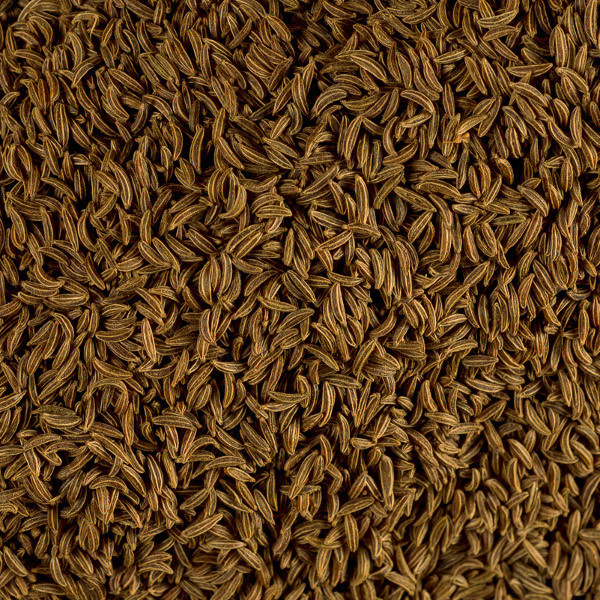
\includegraphics[width=0.33\textwidth]{imgs/spices/caraway-1.jpg}
	\caption{Caraway-seeds (fruits, \textit{Carum carvi}).}
	\label{fig:caraway}
\end{wrapfigure}

Caraway-seeds are in fact the fruits of the plant \textit{Carum carvi}, and they are longer, narrower, and darker than cumin (\textit{Cuminum cyminum}). The two are often confused, both in language and in the kitchen. Caraway hs a visible ``rib'' along the curve that makes the two mericaps (two halves of a compact fruit) better observable \autocite[100]{van_wyk_culinary_2014}. Caraway has a somewhat peppery and bitter, but mild aroma that makes it a popular choice of spice on the vast regions it grows. 

As a spice, caraway is popular in European cuisines, it is used to flavor bread, cheese, sausages, soups, the famous German \textit{sauerkraut} and even alcoholic beverages \autocite{van_wyk_culinary_2014}.

% Caraway has often been confused with the similar-looking cumin, as can be seen in vernacular names that originally referred to cumin (derived from the Latin Cuminum), such as Kümmel (German). Similarly, the Hindi name jeera is sometimes used for caraway but actually refers to cumin and black cumin (see Cuminum cyminum). 



% culinary uses Caraway is a typical spice of German-speaking countries and is an important flavour ingredient of rye bread, sauerkraut, Schweinsbraten (roast pork), goulashes, vegetables, potatoes, cheeses (e.g.,Munster), cakes and biscuits as well as alcoholic beverages such as kümmel, schnapps and vespétro.4 In the Netherlands, it is an ingredient of Leyden cheese, the most common type of kominjekaas. It is also a popular spice in Scandinavia, used to flavour food, confectionery, cheeses (e.g.,Swedish bondost and Danish harvati) and beverages (akvavit). In France, caraway is used to flavour dragées (sugarcoated almonds).4 In Britain it is often included in pickles and cabbage and traditionally served as a condiment (in a small dish) along with baked apples.2 It is popular in confectionery (e.g.,British caraway seedcake and Serbian scones) and desserts (e.g.,Middle Eastern caraway pudding). Flavour compounDs The warm, aromatic flavour of caraway fruits is due to essential oil rich in R-(+)-carvone (60\%) and limonene (40\%)5. S-(–) carvone smells like spearmint and is the main compound of spearmint oil (see Mentha spicata). Only the R-enantiomer of limonene occurs in nature. notes The fruits and essential oil are used to alleviate flatulence and stomach complaints.

% 1. Mabberley, D.J. 2008. Mabberley’s plant-book (3rd ed.). Cambridge University Press, Cambridge. 2. Kiple, K.F., Ornelas, K.C. (Eds). 2000. The Cambridge world history of food. Cambridge University Press, Cambridge. 3. Farrel, K.T. 1999. Spices, condiments and seasonings. Aspen Publishers, Gaithersburg, USA. 4. Larousse. 1999. The concise Larousse gastronomique. Hamlyn, London. 5. Harborne, J.B., Baxter, H. 2001. Chemical dictionary of economic plants. Wiley, New York.

\subsection{The Botany, Origin, and  Cultivation of Caraway}

Similarly to other spice plants in the umbelliferous family, the caraway plant is a small biennial herb with soft stems and umbels of small white flowers that bear the fruits people call seeds \autocite[100]{van_wyk_culinary_2014}. Caraway is indigenous in large areas of Eurasia: central Europe, the Mediterranean region, western and central Asia \autocite{mabberley_mabberleys_2017}. 
% The Romans used the roots as a vegetable. Caraway is now a popular spice in many parts of the world. 
Caraway is widely cultivated in Eastern Europe and German speaking areas, as north as Finland, but the bulk of caraway nowadays comes from Egypt \autocite{farrell_spices_1985}. The plants are grown from seeds, harvesting happens in the second year when the fruits ripen and turn brown \autocite{van_wyk_culinary_2014}.

\subsection{The History of Caraway}

Caraway is an ancient spice as indicated by neolithic samples, and according to \textcite[436]{kiple_cambridge_2000} it was always popular as a local alternative to expensive exotic spices.

\subsection{The Names of Caraway}

\subsubsection{English}

\begin{etymology}\label{ety:caraway}
English \textit{caraway}
< Medieval Latin \textit{carui} `id.', or some allied Romanic form; cf. cognates French carvi, Italian carvi, Spanish carvi (whence Scots carvy, kervie), Old Spanish alcaravea, alcarahueya, Portuguese alcaravia, alcorovia
< Arabic \textit{karawiyā} `id.', (loaned to some Eurropean languages with \textit{al-} definite article; via Andalusian Arabic)
< Aramaic {\he{כַרְוָיָא‎}/\sy{ܟܲܪܘܵܝܵܐ}} \textit{karwāyā} `id.'
< Ancient Greek {καρώ} \textit{karṓ} `id.', a form of the word \textit{káron}, derived from \textit{káre} `head'; -ṓ form seems Pre-Greek (these forms could not immediately give the Arabic, hence possibly via *καρυΐα \textit{*karuḯa} a typical plant derivation form of καρώ \textit{karṓ}, κάρον \textit{káron}); cf. cognates Latin \textit{carum, careum}\footnote{\textcite[s.v. caraway]{oed}; \textcite[s.v. caraway]{ahd}; \textcite[74]{corriente_dictionary_2008}; \textcites[207]{low_aramaeische_1881}[437-438]{low_flora_1924}; \textcites[653]{beekes_etymological_2010}[599]{sokoloff_dictionary_2002}}
\end{etymology}

English \textit{caraway} comes from a Romance language, such as  French \textit{carvi} (attested in 1256)\footcite[carvi]{tlfi} or the equivalent Medieval Latin \textit{carui} (ca. 1080), whence the scientific name.\footcites[caraway]{oed}[carvi]{tlfi} The Romance languages borrowed this word from Arabic \ar{كراويا} \textit{karāwiyā}, sometimes with the definite article \textit{al-}.\footcite{corriente_dictionary_2008} (Many Arabic loanwords in Spanish contain the definite article, and many of these borrowings go back to the times of Muslim Spain in al-Andalus, otherwise know as \textit{La Convivencia}; e.g., \textit{almohada} `pillow', \textit{alcatraz} `cormoran', \textit{alcohol} `alcohol', \textit{álgebra} `algebra', etc.)

The Arabic term has Semitic cognates in Aramaic, which is thought to be a loanword from Ancient Greek \gr{καρώ} \textit{karṓ}, (also etymon of \textit{carrot}), which shows sign of being pre-Greek.\footcite{beekes_etymological_2010}. According to \textcite{sokoloff_dictionary_2002}, the development of the Greek word follows typical plant name derivation patterns. The spice ajowan/ajwain \textit{Trachyspermum ammi} also has a synonym from this etymon: \textit{carom}.

Further English vernacular names use \textit{cumin} as the prototype word, and modify it with distinguishing words that Indicate the general direction and places where caraway was arriving from: the mountainous regions of Armenia and Persia. \textit{Royal cumin}---attested in 1614---seems to be a semantic translation of Hindustani \sa{शाह जीरा}/\fa{شاه جيرا} \textit{shāhjīrā}, a Persianate term that is modeled from the Farsi words \textit{shāh}
`king' (origin of the word \textit{check} in the ``checkmate'' of chess) and \textit{jīrā} `cumin', but its use is restricted to South Asia and not Iran. However, in the first record of it in ``A \lgS hort Table expounding all the hard words in this book'', it refers to bishop's weed, bullwort, or \textit{ammi} (ameos) (\textit{Ammi majus}), which another umbelliferous herb with similar seeds \autocite[]{markham_cheap_1614}.

\begin{table}[!ht]
\centering
\begin{tabularx}{\textwidth}{@{}l>{\itshape \small}lL>{\small}l@{}}
\toprule
\textbf{\#} & \multicolumn{1}{l}{\textbf{Species}} & \multicolumn{1}{l}{\textbf{Name}} & \multicolumn{1}{l}{\textbf{Source}} \\
\midrule
1	& Carum carvi	& Armenian cumin	& \textcite{oed} \\
\textbf{2}	& \textbf{Carum carvi}	& \textbf{caraway}	& \textbf{\textcite{van_wyk_culinary_2014}} \\
3	& Carum carvi	& caraway-seed	& \textcite{oed} \\
4	& Carum carvi	& meredian fennel	& \textcite{wikipedia} \\
5	& Carum carvi	& mountain cumin	& \textcite{oed} \\
6	& Carum carvi	& Persian cumin	& \textcite{wikipedia} \\
7	& Carum carvi	& royal cumin	& \textcite{oed} \\
\bottomrule
\end{tabularx}
\caption{Various names for caraway in English.}
\label{table:names_caraway_en}
\end{table}



\subsubsection{Arabic}

% \begin{etymology}\label{ety:karawiya}
\textbf{Arabic} \textit{karawiyā} `caraway', (loaned to some Eurropean languages with \textit{al-} definite article; via Andalusian Arabic)
< \textbf{Aramaic} {\he{כַרְוָיָא}/\sy{ܟܲܪܘܵܝܵܐ}} \textit{karwāyā} `caraway'
< \textbf{Ancient Greek} {καρώ} \textit{karṓ} `caraway', a form of the word \textit{káron}, derived from \textit{káre} `head'; -ṓ form seems Pre-Greek (these forms could not immediately give the Arabic, hence possibly via *καρυΐα \textit{*karuḯa} a typical plant derivation form of καρώ \textit{karṓ}, κάρον \textit{káron}); cf. cognates Latin \textit{carum, careum}\footnote{\textcite[74]{corriente_dictionary_2008}; \textcites[207]{low_aramaeische_1881}[437-438]{low_flora_1924}; \textcites[653]{beekes_etymological_2010}[599]{sokoloff_dictionary_2002}}
\end{etymology}

The Arabic word for caraway is \ar{كراويا} \textit{karāwiyā}, the etymology of which was discussed under Etymology \ref{ety:caraway}, just above. Caraway was known to the Arabs early on, it appears in the \gls{Hawi}, the monumental tenth-century medical encyclopedia of al-Razi.

\begin{table}[!ht]
\centering
\begin{tabularx}{\textwidth}{@{}l>{\itshape \small}lr>{\itshape}lL>{\small}l@{}}
\toprule
\textbf{\#} & \multicolumn{1}{l}{\textbf{Species}} & \multicolumn{1}{l}{\textbf{Name}} & \multicolumn{1}{l}{\textbf{Tr.}} & \multicolumn{1}{l}{\textbf{Gloss}} & \multicolumn{1}{l}{\textbf{Source}} \\
\midrule
\textbf{1}	& \textbf{Carum carvi}	& \textbf{كراويا}	& \textbf{karāwiyā}	& \textbf{}	& \textbf{\textcite{wehr_dictionary_1976}} \\
\bottomrule
\end{tabularx}
\caption{Various names for caraway in Arabic.}
\label{table:names_caraway_ar}
\end{table}



\subsubsection{Chinese}

\begin{etymology}\label{ety:geluzi}
\textbf{Mandarin Chinese} \traditionalchinesefont{葛縷子} \textit{gě​lǚ​zi} `caraway' [bean-hemp-seed?], phono-semantic matching; see \textit{shilo} `cumin and caraway'
< \textbf{Japanese} \traditionalchinesefont{葛縷子} \textit{karyuushi} `caraway', probably a transcription of Latin \textit{Carui}, or English \textit{caraway} + \textit{zi} (also キャラウェイ \textit{kyarawei} and \traditionalchinesefont{姫茴香} [princess-fennel-spice]), 1822
<\textss{?} from \textbf{English} \textit{caraway} `caraway', ca. 1440
 or from \textbf{Medieval Latin} \textit{carui} `caraway', or some allied Romanic form; cf. cognates French carvi, Italian carvi, Spanish carvi (whence Scots carvy, kervie), Old Spanish alcaravea, alcarahueya, Portuguese alcaravia, alcorovia
< \textbf{Arabic} {كراويا} \textit{karāwiyā} `caraway', (loaned to some Eurropean languages with \textit{al-} definite article; via Andalusian Arabic)
< \textbf{Aramaic} {\he{כַרְוָיָא}/\sy{ܟܲܪܘܵܝܵܐ}} \textit{karwāyā} `caraway'
< \textbf{Ancient Greek} {καρώ} \textit{karṓ} `caraway', a form of the word \textit{káron}, derived from \textit{káre} `head'; -ṓ form seems Pre-Greek (these forms could not immediately give the Arabic, hence possibly via *καρυΐα \textit{*karuḯa} a typical plant derivation form of καρώ \textit{karṓ}, κάρον \textit{káron}); cf. cognates Latin \textit{carum, careum}\footnote{\textcite[100]{kleeman_oxford_2010}; \textcite[s.v. caraway]{oed}; \textcite[s.v. caraway]{ahd}; \textcite[74]{corriente_dictionary_2008}; \textcites[207]{low_aramaeische_1881}[437-438]{low_flora_1924}; \textcites[653]{beekes_etymological_2010}[599]{sokoloff_dictionary_2002}}
\end{etymology}

In Chinese, the modern word for caraway is \tc{葛縷子} \textit{geluzi}, but this does not appear in historical documents or corpora. We know from \textcite{laufer_sino-iranica_1919} and \textcite{schafer_golden_1985} that caraway was not distinguished from cumin, and the same words were used for both. An any case, the first record of this word is from a 1822 Japanese book on Western medicinal products, where it appears to be the rendering of the Latin name \textit{carui}, probably informed by English \textit{caraway} (in modern Japanese caraway is \jp{キャラウェイ} \textit{kyarawei} and \jp{姫茴香} [princess-fennel-spice]). The kanjis in the 1822 book are annotated with a katakana reading of \jp{カリュイ} \textit{karyui}. I can not say for certain that Chinese loaned the Japanese term, but until I come across nineteenth-century attested forms in Chinese publications, I will assume so.

\begin{table}[!ht]
\centering
\begin{tabularx}{\textwidth}{@{}l>{\itshape \small}ll>{\itshape}lL>{\small}l@{}}
\toprule
\textbf{\#} & \multicolumn{1}{l}{\textbf{Species}} & \multicolumn{1}{l}{\textbf{Name}} & \multicolumn{1}{l}{\textbf{Tr.}} & \multicolumn{1}{l}{\textbf{Gloss}} & \multicolumn{1}{l}{\textbf{Source}} \\
\midrule
\textbf{1}	& \textbf{Carum carvi}	& \textbf{\tradchinesefont{葛縷子}}	& \textbf{gě​lǚ​zi}	& \textbf{phonetic?}	& \textbf{\textcite{kleeman_oxford_2010}} \\
2	& Carum carvi	& \tradchinesefont{頁蒿}	& yèhāo	& leaf-wormwood	& \textcite{mdbg} \\
3	& Carum carvi	& \tradchinesefont{藏茴香}	& zànghuíxiāng	& Tibetan-hui-spice	& \textcite{mdbg} \\
\bottomrule
\end{tabularx}
\caption{Various names for caraway in Chinese.}
\label{table:names_caraway_zh}
\end{table}



\subsubsection{Summary}

\begin{table}[!ht]
\centering
\begin{tabularx}{\textwidth}{@{}ll>{\itshape}lLl>{\small}l@{}}
\toprule
\textbf{\#} & \textbf{Language} & \multicolumn{1}{l}{\textbf{Term}} & \textbf{Gloss} & \textbf{Loan} & \multicolumn{1}{l}{\textbf{Source}} \\
\midrule
1	& English	& Armenian cumin	& 	& no	& \textcite{oed} \\
2	& English	& caraway	& 	& yes	& \textcite{oed} \\
3	& English	& caraway-seed	& 	& no	& \textcite{oed} \\
4	& English	& mountain cumin	& 	& no	& \textcite{oed} \\
5	& English	& royal cumin	& 	& no	& \textcite{oed} \\
\midrule
1	& Arabic	& karāwiyā	& 	& yes	& \textcite{wehr_dictionary_1976} \\
\midrule
1	& Chinese	& gělǚzi	& 	& yes	& \textcite{kleeman_oxford_2010} \\
2	& Chinese	& yèhāo	& leaf-wormwood	& no	& \textcite{mdbg} \\
3	& Chinese	& zànghuíxiāng	& Tibetan-hui-spice	& no	& \textcite{mdbg} \\
\bottomrule
\end{tabularx}
\caption{Conventionalized names for caraway in English, Arabic, and Chinese, found in dictionaries.}
\label{table:names_caraway}
\end{table}




% \clearpage % % Full page illustration
% \begin{figure}[!hbtp]
%     \centering
%     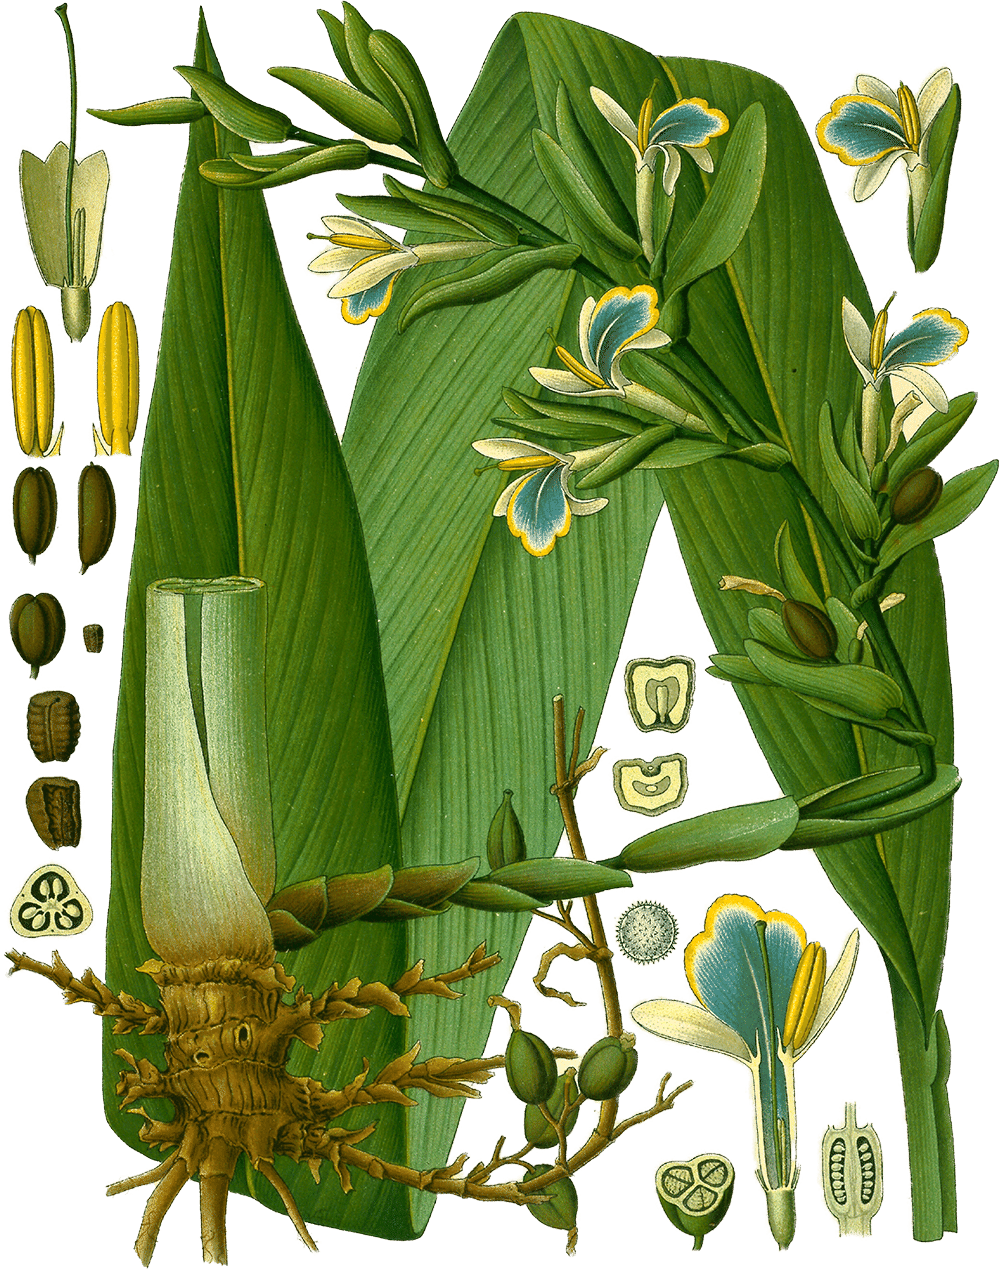
\includegraphics[width=\textwidth]{imgs/kohler/cardamom_kohler_min.png}
%     \caption{\taxonn{Elettaria cardamomum}{(L.) Maton} (syn. \taxonn{Amomum cardamomum}{L.}), the cardamom plant in Köhler's Medicinal Plants \pvolcite[]{2}[186]{kohler_kohlers_1887}.}
%     \label{fig:kohler_cardamom}
% \end{figure}



\section{Cardamom}
\label{sec:cardamom}\label{sec:black_cardamom}

\begin{spice}\label{spice:cardamom}
\textsc{Cardamom} \hfill \href{https://powo.science.kew.org/taxon/796556-1}{POWO} \\
\textbf{English:} \textit{cardamom}. 
\textbf{Arabic:} {\arabicfont{هال}} \textit{hāl}; {هيل} \textit{hayl}. 
\textbf{Chinese:} {\tradchinesefont{豆蔻}} \textit{dòukòu} [bean-cardamom]; 荳蔻. 
\textbf{Hungarian:} \textit{kardamom}.  \\
\noindent{\color{black}\rule[0.5ex]{\linewidth}{.5pt}}
\begin{tabular}{@{}p{0.25\linewidth}@{}p{0.75\linewidth}@{}}
Plant species: & \taxonn{Elettaria cardamomum}{(L.) Maton} (syn. \taxonn{Amomum cardamomum}{L.}) \\
Family: & \textit{Zingiberaceae} \\
part used: & fruit (seed pods, capsules) \\
Region of origin: & India \\
Cultivated in: & Guatemala; India; Sri Lanka; Tanzania; Papua New Guinea \\
Color: & green seed pods, brown seeds \\
\end{tabular}
\end{spice}

\begin{figure}[!ht]
	\vspace{-2ex}
	\centering
	\subfloat{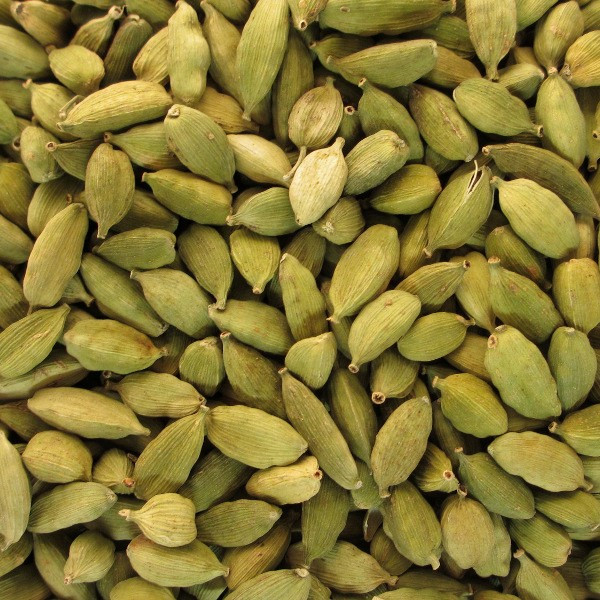
\includegraphics[width=0.3\linewidth]{imgs/spices/cardamom-1.jpg}}
	\hfill
	\subfloat{\includegraphics[width=0.3\linewidth]{imgs/spices/cardamom-2.jpg}}
	\hfill
	\subfloat{\includegraphics[width=0.3\linewidth]{imgs/spices/cardamom-3.jpg}}
	\caption[True cardamom]{Cardamom fruits cured, and powdered (\taxon{Elettaria cardamomum}). Credit: Aromatiques.}
	\label{fig:cardamom_imgs}
\end{figure}

Cardamoms are the dried, ripe fruits of the cardamom plant \taxon{Elettaria cardamomum}. These fruits are sometimes called seeds, but they are in fact the seed pods, ``three-valved capsules'' \autocite[132]{van_wyk_culinary_2014}, containing several brown-colored small seeds, as it can be seen in \cref{fig:cardamom_imgs}. The cardamom of commerce is widely used in Asia as medicine and spice, and is valued for its unique, minty and eucalyptus-like flavor. It is most prevalent in Indian cooking, but also known from the Arabic coffee tradition where it is sometimes added to the beverage. Indian restaurants often place a bowl of cardamoms at the entrance, so customers can take one as a masticatory on their way out, and chew on the refreshing capsules as they were nature's breath mints. Native to the same region as the mighty black pepper in India, cardamom is sometimes referred to as the ``queen of spices'' \autocite[1]{ravindran_cardamom_2002}. Cardamom was imported to Europe since the Roman era, and it is still used in meat dishes, sausages, Swedish meatballs, Danish pastries, ice-cream and liqueurs \autocite[326]{mabberley_mabberleys_2017}. It is the third most expensive spice of our times, after saffron and vanilla \autocite{business_insider_why_2021}.

Although \textit{cardamom} usually refers to the fruits of \taxon{E. cardamom} from India---also sometimes known as green cardamom and true cardamom---there are numerous other cardamoms, similarly segmented capsule-like fruits used as spices and medicine in South, Southeast, and East Asia, and even in Africa. Many of these belong to the \taxon{Amomum} genus of the ginger family (\taxon{Zingiberaceae}), such as the black cardamom from the Himalayas (\taxon{Amomum subulatum}), and the round cardamom from Java (\taxon{Amomum compactum}). See them in detail below in \cref{sec:crowd_of_cardamoms}.

% Aromatiques:

% Elettaria cardamomum

% Green cardamom, "queen of spices" in India, is indeed one of the most original and enchanting ones. From the zingiberaceae family, this beautiful plant is grown mainly in India, Sri Lanka or Guatemala. Naturally green and perfumed, the pods are only dried. Their powerful fragrance is very aromatic, hot and peppery but also camphor and menthol, durable and slightly numbing, making it a sovereign spice. We sometimes find white cardamom, these are the same pods, originally green, discoloured with sulfur and soap baths for an aesthetic purpose, they are less aromatic than green ones. Cardamom is used, either peeled: by opening the fruit to release the small black-grey seeds to be mortared (10-20 per pod); or whole in infusion in simmered dishes or cooking water.

% Traditionally used in Indian cuisine, green pods are an essential element of many dishes such as curry, dhal, rice. Cardamom powder is also present in classic mixtures such as masal garam or some curries. In sweet and savoury we find it in chutneys recipes. In Europe, cardamom is associated in salted with charcuterie or fish.

% Desserts are also greatly improved by cardamom: fruit salads, cakes, lassis, ice cream, gingerbread. It goes perfectly with chocolate: mousse, fondant, ice cream...

% Green cardamom is used in several traditional drinks in different parts of the world: it is added to coffee in the Middle East, mixed with other spices to prepare chaï masala in India, mulled wine in Europe or hypocras since the Middle Ages. It is also an ingredient of choice for flavoring punch and rhum arrangé.

% Chewing green cardamom seeds is very pleasant and refreshes the breath thanks to its fresh and minty aroma. It is also possible to neutralize the stubborn smell of garlic by this means.

% Cardamom has been recognized for millennia in Indian Ayurvedic medicine and Chinese medicine for its anti-acide, carminative, stomachic, appetizer and anti-nausea digestive properties.

% Amomum subulatum

% Also known as cardamom from China or Nepal, or fake cardamom, these large brown pods have a strong smoky scent and a very pronounced camphor taste. Smoked in wood fire, the coarse shell that contains the seeds concentrates essentially this smoky aroma, so we keep the whole pod, with its bark, to benefit the best in the kitchen. We only keep the seeds, possibly crushed in a mortar, if we want to highlight the camphor flavor

% Brown cardamom is mainly used as a spice in the preparation of Indian curry and other savory dishes from India that simmer for a long time. It is also associated with green cardamom in some recipes. To be added to chickpea, coral lentil or potato dishes to give a slightly raw and woody note.


% WIKI
%     True or green cardamom (or when bleached, white cardamom[12]) comes from the species Elettaria cardamomum and is distributed from India to Malaysia. What is often referred to as white cardamon is actually Siam cardamom, Amomum krervanh.[13]
%     Black cardamom, also known as brown, greater, large, longer, or Nepal cardamom, comes from species Amomum subulatum and is native to the eastern Himalayas and mostly cultivated in Eastern Nepal, Sikkim, and parts of Darjeeling district in West Bengal of India, and southern Bhutan.

% The two types of cardamom, καρδάμωμον and ἄμωμον, were distinguished in the fourth century BCE by Theophrastus. He reports that some people believed they came from Media, others from India.[14] 


% wiki:
% Amomum subulatum, also known as Black cardamom, hill cardamom,[1] Bengal cardamom,[1] greater cardamom,[1] Indian cardamom,[1] Nepal cardamom,[1] winged cardamom,[1] big cardamon,[2][3] or brown cardamom, is a perennial herbaceous plant in the family Zingiberaceae. Its seed pods have a strong, camphor-like flavour, with a smoky character derived from the method of drying. In Hindi it is called बड़ी इलाइची (baḍī ilāichī).
% Contents

%     1 Characteristics
%     2 Species
%     3 Medical production
%     4 See also
%     5 References

% Characteristics

% The pods are used as a spice, in a similar manner to the green Indian cardamom pods, but with a different flavour. Unlike green cardamom, this spice is rarely used in sweet dishes. Its smoky flavour and aroma derive from traditional methods of drying over open flames.
% Species

% At least two distinct species of black cardamom occur: Amomum subulatum (also known as Nepal cardamom) and Amomum tsao-ko. The pods of A. subulatum, used primarily in the cuisines of India and certain regional cuisines of Pakistan, are the smaller of the two, while the larger pods of A. tsao-ko (Chinese: wiktionary:草果; pinyin: cǎoguǒ; Vietnamese: thảo quả) are used in Vietnamese cuisine and Chinese cuisine, particularly that of Sichuan province.
% Medical production

% The largest producer of the black cardamom is Nepal, followed by India and Bhutan. In traditional Chinese medicine, black cardamom is used for stomach disorders and malaria.[dubious – discuss] In the traditional medicine of India, decoction of Amomum subulatum rhizomes is used in the therapy of jaundice.[4] 

\subsection{The Botany, Origins, and Cultivation of Cardamom}

The cardamom plant is a tall perennial herb from the ginger family (\taxon{Zingiberaceae}) with pink white flowers that grow at the base of the stem in clusters \autocite[132]{van_wyk_culinary_2014}. \taxon{Elettaria cardamomum} is indigenous to the Western Ghats region in South India, the same area that gave us black pepper and the center of its production and biodiversity \autocite[1]{ravindran_cardamom_2002}. Together with black pepper and ginger, it has been wild-harvested since time immemorial, and formed the livelihood of many from the beginnings of the ancient spice trade around the \nth{3} century \BC{}, until today \autocite[132]{van_wyk_culinary_2014}. Cardamom can only grow in a tropical climate, thriving in higher altitudes in the shade of trees, similarly to black pepper (which is a climbing vine) and thus modern cultivation does not differ much from traditional wild harvesting \autocite[132]{van_wyk_culinary_2014}. Cardamom is hand picked when ripe or near-ripe one by one---explaining its relatively high price---and then dried. It generally comes in light green, but one can also find them in white, which is a result of an extra step of steaming or bleaching before the drying process \autocite[132]{van_wyk_culinary_2014}. From the 1920s, Guatemala gradually became a major cardamom exporter, surpassing India in production. It is also grown in Tanzania and Papua New Guinea on a small scale.

\subsection{The History of Cardamom}

It is difficult to trace the history of cardamoms with certainty because of the confusion in nomenclature \autocite{cumo_encyclopedia_2013}. However, the cardamom described in \nth{4} century \BC{} in Indian Ayurvedic literature is probably the green or true cardamom of today, called \textit{el\={a}}\footcite[232]{monier-williams_sanskrit-english_1899} in Sanskrit. Cardamom was also described by Theophrastus in the \nth{4} century \BC{}. He reports that \textit{kardamomon} and \textit{amomon} (cardamom and black cardamom) come from Media, or according to some, from India---just like spikenard and most other spices \autocite[249]{theophrastus_enquiry_1916}. Pliny connects amomum to North India, which is quite a punctual source for black cardamom. Cardamom was known to Dioscorides and Hippocrates, who have both written on its health benefits, e.g. aiding digestion. In Modern Greek, there is an informal way of saying `to strengthen, get strong': \gr{καρδαμώνω} \textit{kardamóno}\footnote{\url{https://www.greek-language.gr/greekLang/modern_greek/tools/lexica/triantafyllides/search.html?lq=\%CE\%BA\%CE\%B1\%CF\%81\%CE\%B4\%CE\%B1\%CE\%BC\%CF\%8E\%CE\%BD\%CF\%89\&dq=}} deriving from the name of the spice.

Medieval Arab doctors wrote about cardamom in similar ways, and the geographer al-Idrīsī described  ca. 1150 that it is brought to the port of Aden from Sindh, India and China, whereas in China, black cardamoms were important in the economy of the Song period (960–1279) \autocite[158-159]{prance_cultural_2005}. Green cardamom reached China from Southeast Asia, in Hong Kong it is consumed primarily by the Indians and the Portuguese. It is cultivated in Guangdong, Guangxi, and Yunnan, rather used in medicine than cooking \autocite[325-326]{hu_food_2005}. For more on cardamom's history, see \textcite[102-106]{dalby_dangerous_2000}.

% USES
% wyk
% culinary uses The delicious sweetish and pungent taste of cardamom has found its way into many different culinary traditions. In its native India, cardamom forms an important component of curries and curry powders. It is also widely used in rice, vegetable and meat dishes, as well as sweet desserts. The seeds are traditionally used to flavour Arabian coffee and black Turkish tea.3 In Europe and America, cardamom is well known as an essential ingredient of gingerbread and sweet pastries. Scandinavians (especially Swedes and Finns) are particularly fond of cardamom and large amounts are used in confectionery, desserts, stewed fruits, mulled wines, meat dishes and sausages.3 Ground cardamom is added to hamburger patties and meatloaf – one teaspoon per kg (2.2 lb.), while roughly bruised seeds are used in sausages as well as in breads, buns and brioches.3 Flavour compounDs The essential oil contains 1,8-cineole (eucalyptol) and α-terpinyl acetate as major compounds, but the typical aroma of cardamom is ascribed to trace amounts of unsaturated aliphatic aldehydes such as (E)-4-decenal.4 notes For Ethiopian cardamom (korarima), see Aframomum corrorima.

\subsection{A Crowd of Cardamoms: Identity and Confusion with Other Spices}
\label{sec:crowd_of_cardamoms}

% \begin{spice}\label{spice:black cardamom}
\textsc{Black cardamom} \hfill \href{https://powo.science.kew.org/taxon/urn:lsid:ipni.org:names:872166-1}{POWO} \\
\textbf{English:} \textit{black cardamom}; \textit{brown cardamom; greater cardamom; Indian cardamom; Nepal cardamom; Indian black cardamom; Bengal cardamom; big cardamom; hill cardamon; winged cardamom; fake cardamom; false cardamom; amomum*}. 
\textbf{Arabic:} {\arabicfont{قاقلة}} \textit{qāqulla}. 
\textbf{Chinese:} {\tc{香豆蔻}} \textit{xiāngdòukòu} [fragrant-cardamom]; \tc{嘎哥拉} \textit{gāgēlā}. 
\textbf{Hungarian:} \textit{fekete kardamom} [black cardamom].  \\
\noindent{\color{black}\rule[0.5ex]{\linewidth}{.5pt}}
\begin{tabular}{@{}p{0.25\linewidth}@{}p{0.75\linewidth}@{}}
Plant species: & \taxonn{Amomum subulatum}{Roxb.} \\
Family: & \textit{Zingiberaceae} \\
Plant part used: & fruit & seed \\
Region of origin: & Nepal to Central China \\
Cultivated in: & Himalayas \\
Color: & dark brown \\
\end{tabular}
\end{spice}

%picture of red cardamom and korarima?

\begin{figure}[!ht]
	\vspace{-2ex}
	\centering
	\subfloat[]{\includegraphics[width=0.3\linewidth]{imgs/spices/cardamom-black-1.jpg}}
    \hfill
	\subfloat[]{\includegraphics[width=0.3\linewidth]{imgs/spices/cardamom-chinese-1.jpg}}
    \hfill
	\subfloat[]{\includegraphics[width=0.3\linewidth]{imgs/spices/cardamom-white-1.jpg}}
	\caption[False cardamoms]{False cardamoms: (a) Black cardamom from the Himalayas (\taxon{Amomum subulatum}), (b) Chinese black cardamom or \textit{tsao-ko} from Yunnan, China (\taxon{Amomum tsao-ko}), and (c) round cardamom from Java (\taxon{Amomum compactum}). Credit: Aromatiques, NAI.}
	\label{fig:black_cardamom_imgs}
\end{figure}

When it comes to cardamoms most of us are only familiar with one or two kinds, however, there is a multitude of plant species that are harvested for their fruit known by their common names as some kind of cardamom. All of these belong to \taxon{Zingiberaceae}. True cardamom---commercially the most important species---belongs to the genus \taxon{Elettaria}, a name derived from the Tamil root \textit{elettari}, meaning cardamom seeds \autocite[1]{ravindran_cardamom_2002}. Besides the genus \textit{Elettaria}, ``false'' cardamoms are found in two other genera: \taxon{Amomum} and \taxon{Aframomum}. Following \textcite[290-308]{van_wyk_culinary_2014}'s checklist, these are listed in \cref{table:amomum_aframomum}.

% >{\small}

\begin{table}[!ht]
\centering
\begin{tabularx}{\linewidth}{@{}lXl@{}}
\toprule
\taxon{Amomum aromaticum} & Bengal cardamom; Nepal card.; large card. & Bangl.; Nepal \\
\taxon{Amomum compactum}⁑ & Indonesian cardamom & SE. Asia \\
\taxon{Amomum costatum}* & Chinese black cardamom & E. Asia \\
\taxon{Amomum globosum} & round Chinese cardamom & China \\
% \taxon{Amomum gracile} & slender cardamom & Southeast Asia, leaf
\taxon{Amomum kepulaga}⁑ & round cardamom & Trop. Asia \\
\taxon{Amomum krervanh} & Cambodian cardamom; krervanh & Trop. Asia \\
\taxon{Amomum maximum} & Java cardamom & Trop. Asia \\
% \taxon{Amomum ochreum} & tepus batu & Asia \\
\taxon{Amomum subulatum} & brown cardamom; greater card.; Indian card. & Asia \\
% \taxon{Amomum testaceum} & ka tepus & Asia \\
\taxon{Amomum tsao-ko}* & tsao-ko cardamom; large cardamom & Asia \\
\taxon{Amomum villosum} & Malabar cardamom; Tavoy card.; wild Siamese card. & Asia \\
\taxon{Amomum xanthioides} & bastard Siamese cardamom; wild Siamese card. & Asia \\
% \taxon{Amomum xanthophlebium} & elach & Asia, flower \\
% \midrule
\taxon{Aframomum alboviolaceum} & Cameroon cardamom & Trop. Africa \\
\taxon{Aframomum angustifolium} & Madagascar cardamom & Madagascar \\
\taxon{Aframomum daniellii} & bastard Melegueta; Cameroon cardamom & Trop. W. Af. \\
% \taxon{Aframomum exscapum} & alligator pepper; grains of paradise & Trop. W. Af. \\
% \taxon{Aframomum granumparadisi} & grains of paradise & W. Af. \\
\taxon{Aframomum hanburyi} & Cameroon cardamom & Trop. W. Af. \\
\taxon{Aframomum corrorima} & Ethiopian cardamom; korarima & Trop. NE. Af. \\
\taxon{Aframomum macrospermum} & Guinea cardamom & W. Af. \\
% \taxon{Aframomum melegueta} & Melegueta pepper; grains of paradise; alligator pepper & Trop. West Africa \\
% \taxon{Aframomum sceptrum} & black amomum & W. Africa \\
\bottomrule
\end{tabularx}
\caption[Cardamoms in the genera \taxon{Amomum}, and \taxon{Aframomum}.]{Spice plants with a common name that includes \textit{cardamom} from the \taxon{Amomum} genus in Asia cultivated for their fruit \& seed, and those from the \taxon{Aframomum} genus of Africa, cultivated for their seed \autocite{van_wyk_culinary_2014}. Items marked with asterisks are identified as botanical synonyms by me.}
\label{table:amomum_aframomum}
\end{table}

\taxon{Amomum}\footcite[Amomum Roxb. \link{https://www.gbif.org/species/7434655}]{gbif} is a genus home to a remarkable number of plants that yield pungent fruits and seeds, most known for \taxon{Amomum subulatum}. The \taxon{Amomum} genus contains of dozens of aromatic, spice-yielding and medicinal plant species primarily growing in India and China, and elsewhere in tropical and subtropical Asia, New Guinea, and North Queensland. Commonly called black cardamom or brown cardamom, but also referred to in various other names in English, such as Nepal cardamom, greater cardamom, Indian cardamom, Indian black cardamom, fake cardamom, Bengal cardamom, big cardamom, hill cardamon, and winged cardamom, the fruits of \taxon{A. subulatum} are larger than green cardamom, and it is native to the eastern Himalayan region; North India, Nepal, Bhutan, and Tibet. In Hindi it is called \hi{बड़ी इलाइची}
\textit{baḍī ilāichī} `big cardamom' or \hi{काली इलाइची}
\textit{k\={a}lī ilāichī} `black cardamom'. In Chinese it is known as \tc{香豆蔻} \textit{xiāngdòukòu} `fragrant cardamom', and \textcite[327]{hu_food_2005} also reports a local name in eastern Tibet for it: \zh{嘎哥拉} \textit{gágēlā} (ka-ko-la), which we will return to later. The dried fruits of this plant (see \cref{fig:black_cardamom_imgs}) are used in savory dishes of northern India and Pakistan, and have a heavy smoky aroma and camphor-like taste. The brown color is a result of roasting and smoking on open fires \autocite[132]{van_wyk_culinary_2014}.

There are even larger (black) cardamoms, growing in the mountainous Vietnam-China borderlands, important in the cuisines of Vietnam, Yunnan, and Sichuan, such as \taxon{A. tsao-ko}\footnote{\url{https://herbaltcm.sn.polyu.edu.hk/herbal/caoguo}} (recently renamed as \taxonn{Lanxangia tsao-ko}{(Crevost \& Lemarié) M.F.Newman \& Skornick.}), which \textcite[326]{hu_food_2005} calls Yunnan cardamom, and explains that in Yunnan, it goes into the chicken soup whole, as a flavoring agent. It is also used medicinally\footnote{\gls{FOC}---\url{http://www.efloras.org/florataxon.aspx?flora_id=2&taxon_id=240001100}}, and the scientific species name comes from the transcribed Chinese name \zh{草果} \textit{cǎoguǒ}. In English it is called \textit{tsao-ko cardamom}. \textcite[326]{hu_food_2005} distinguishes an \taxonn{A. hongtsaoko}{Liang et Fang} (red cardamom), which appears to be a synonym for \taxon{A. tsaoko} after consulting botanical databases. If one searches for ``red cardamom'' online, spice vendors' advertisements would appear offering tsao-ko cardamom, also named ``cao guo''. \textcite{putzel_spice_2017} calls tsao-ko cardamom simply as black cardamom, and explores its cultivation and trade in Yunnan in great detail. He explains that in the last 50 years it has become a cash crop, and it is now the primary source of cardamom in Yunnan, together with \taxon{A. villosum}\footnote{\url{https://herbaltcm.sn.polyu.edu.hk/herbal/villous-amomum-fruit}}, known as Tavoy cardamom, or \zh{砂仁} \textit{shārén} in Chinese \autocite[41]{putzel_spice_2017}.

Lastly, there are cardamoms that are round and white, indigenous to Southeast Asia. \taxon{Amomum krervanh} (newly reassigned as \taxonn{Wurfbainia vera}{(Blackw.) Skornick. \& A.D.Poulsen}) is Siam cardamom, Cambodian cardamom, or krervanh in English, and \tc{白豆蔻} \textit{báidòukòu} `white cardamom' in Chinese. \taxon{A. compactum} (newly reassigned as \taxonn{Wurfbainia compacta}{(Sol. ex Maton) Skornick. \& A.D.Poulsen} is known as round cardamom, Indonesian cardamom, or Java cardamom in English, and \tc{爪哇白豆蔻} \textit{Zhǎowā báidòukòu} `Java white cardamom' in Chinese, a spice used in \gls{TCM}, and botanically very similar to \taxon{A. maximum}, which is \tc{九翅豆蔻} \textit{jiǔchìdòukòu} `nine-winged cardamom' in Chinese. These are the first cardamoms that were imported to China from mainland Southeast Asia, together with nutmegs that caused an initial confusion we will shortly see. Cardamom in Indonesian is called \textit{kapulaga} (Javanese \jv{ꦏꦥꦸꦭꦒ} 
\textit{kapulaga}), primarily referring to \taxon{A. compactum} (more specifically \textit{kapulaga jawa} `Javanese cardamom', with an Old Javanese word\footnote{\gls{SEAL}---\url{http://sealang.net/ojed/index.htm}} that people on the Wiktionary try to connect with Sanskrit \sa{कक्कोल} \textit{kakkola} \footcite[241. \link{https://www.sanskrit-lexicon.uni-koeln.de/scans/MWScan/2020/web/webtc2/index.php}]{monier-williams_sanskrit-english_1899}. Wyk's \taxon{A. kepulaga} is a synonym for \taxon{A. compactum}.

Moving on to Africa, the genus \taxon{Aframomum}\footcite[Aframomum K.Schum. \link{https://www.gbif.org/species/2758799}]{gbif} contains around 50 species from the tropical regions of Africa, including Madagascar, Mauritius, and the Seychelles on the Indian ocean. The most important spice crop of this genus is \taxon{Aframomum melegueta} (grains of paradise, Melegueta pepper), and \taxon{A. exscapum} (alligator pepper), and staying on cardamoms: \taxon{A. corrorima}, commonly known as Ethiopian cardamom, or korarima. The latter is also often referred to as false cardamom, because the structure of the fruit imitates the true cardamom. One difference between the African and Asian cardamoms, is that in Africa, mostly the seeds are used, while in Asia, the whole seed pods are made use of \autocite{van_wyk_culinary_2014}.



What is common in all these different spice plants spanning from Asia to Africa? What connects them and makes us discuss them under cardamom? Their physical (and biochemical) properties. Not only are these plants related botanically, but the anatomy of their fruits are quite similar. Consequently, we can deduct that cardamom as a prototype has two features: (1) it is aromatic, (2) it is a capsule containing edible seeds. And just as cardamom is a prototypical object, \textit{cardamom}---as a name---is a prototypical word that is used and reused as a headword to propagate spice names. There is also a certain dichotomy at play, the dynamics of adjectives that describe, distinguish, and evaluate a type of cardamom. Think of: green vs. black, Indian vs. Nepal, lesser vs. greater, true vs. false.

\subsubsection{Some Remarks on Common Names}

When combing through the literature of cardamoms, there is small degree of conflict and overlap in the English common names that authors give to a plant and its spice. The vernacular names contend each other because authors come from different backgrounds, where one name might exist, but another does not, and---as mentioned in the introduction of this thesis---there are no rules governing this; it is up to each author. Scholars such as \citeauthor{van_wyk_culinary_2014} from South Africa, \citeauthor{ravindran_cardamom_2002} from India, and \citeauthor{hu_food_2005} from China all bring a layer of diversity to the discussion of spices with their mentions and omissions of various common names of the plants/spices they so systematically try to present. This is expected, writers with a botanical focus pay attention to the strictly regulated scientific names in plant identification, so sometimes the included and excluded vernacular names are chosen on a whim, or depend on how much space is there left on the page. Some authors just note one common name, while some try to include as many as there are. A more interesting question would be: how do authorities on plant science go about the selection process? Where do they gather the vernacular names from?

Often, botanical and gastro writers have to make up what I call ``speculative names'', where an author feels the need to devise/translate a common name for a plant that does not necessarily exist in the target language they write. In this section, \textit{red cardamom} is certainly a case on point. This is not a judgment, rather an observation; sometimes these inventions come to life and begin their journey as ``real'' plant/spice names that people will use if it fills a need. Further examples are found in \textcite[64]{raghavan_handbook_2007}, who calls allspice \textit{English spice} in English, which is an obvious translation from other languages that do in fact call it ``English spice'' (for the English fleet disseminated it from their colony of Jamaica).

\subsection{The Names of Cardamom}

\subsubsection{English}

\begin{etymology}\label{ety:cardamom}
English \textit{cardamom} `cardamom', (via post-classical Latin \textit{cardimomum}, a. 1398), ?ca. 1425
< later also from Old French \textit{cardemome} `cardamom', ca. 1170; cf. modern French \textit{cardamome}
< Latin \textit{cardamōmum} `cardamom', \nth{1} c. \AD{}
< Hellenistic Greek {καρδάμωμον} \textit{kardámōmon} `cardamom', haplological \gr{κάρδαμ-} \textit{kárdam-} `cress' + \gr{ἄμωμον} \textit{ámōmon} `an Indian spice plant', \nth{3} c. \BC{}
< Ancient Greek {κάρδαμον} \textit{kárdamon} `garden cress \taxon{Lepidium sativum}', prehaps a loanword (many plant names with \textit{-amon} are clear loanwords; the suffIx \textit{-amon} is known from Pre-Greek), \nth{4} c. \BC{}; cf. cognates classical Latin \textit{cardamum}
<\textss{?} unknown \textit{*}\footnote{\textcite[s.v. cardamom]{oed}; \textcite[s.v. cardamome]{tlfi}; \textcite[s.v. cardamomum]{lewis_latin_1879}; \textcite[s.v. καρδάμωμον]{liddell_greek-english_1940}; \textcite[s.v. κάρδαμον]{liddell_greek-english_1940}; \textcite[644]{beekes_etymological_2010}}
\end{etymology}

\begin{table}[!ht]
\centering
\begin{tabularx}{\textwidth}{@{}l>{\itshape \small}lL>{\small}l@{}}
\toprule
\textbf{\#} & \multicolumn{1}{l}{\textbf{Species}} & \multicolumn{1}{l}{\textbf{Name}} & \multicolumn{1}{l}{\textbf{Source}} \\
\midrule
\textbf{1}	& \textbf{Elettaria cardamomum}	& \textbf{cardamom}	& \textbf{\textcite{van_wyk_culinary_2014}} \\
2	& Elettaria cardamomum	& green cardamom	& \textcite{ravindran_cardamom_2002} \\
3	& Elettaria cardamomum	& true cardamom	& \textcite{ravindran_cardamom_2002} \\
\bottomrule
\end{tabularx}
\caption{Various names for cardamom in English.}
\label{table:names_cardamom_en}
\end{table}



The word \textit{cardamom} came from Latin \textit{cardamōmum} via a Late Latin form attested in the late \nth{14} century, and was later also influenced by French \textit{cardamome}, which has the same Latin etymon. \textit{Cardamōmum} is the Latinized form of Greek \gr{καρδάμωμον} \textit{kardámōmon}, a word that was formed by compounding the Ancient Greek \gr{κάρδαμον} \textit{kárdamon} `cress', which is of unknown origin, and \gr{ἄμωμον} \textit{ámōmon} `amomum', signifying an unidentified Indian spice plant, formed with haplology (\textit{*kardamamōmom}). \footcites[cardamom]{oed}[cardamom]{ahd} The \gls{OED} also lists many other European cognates of the English word, such as Spanish \textit{cardamomo} (mid \nth{13} c. or earlier), Italian \textit{cardamomo} (late \nth{13} c.), and Middle High German \textit{kardamōm} (\nth{13} c., modern German \textit{Kardamom}).
In some cases, the form shows a dissimilation of the two final nasals, and so we can come across forms, such as \textit{cardamon}.

% ``Cardamomum [...] the better is some deale réd with sharp sauour medled with swéetnesse, and hath vertue to comfort and to wast, \& helpeth therefore against the Cardiacle passion, \& against wamblings and indignation of the stomacke, and exciteth appetite, and abateth spuing, and comforteth féeble braine, as Dioscorides and Platearius say.'' \autocite[\link{https://quod.lib.umich.edu/e/eebo/A05237.0001.001/1:28.33?rgn=div2;view=fulltext}]{bartholomaeus_batman_1582}

\textcite[644]{beekes_etymological_2010} does not speculate on the origin of \textit{kárdamon}, but explains that plant names ending in \textit{-amon} are clearly and frequently loanwords, and that the suffix \textit{-anon} is a known pre-Greek element. He also mentions some doubtful attempts to explain the word by previous authors, and mentions that it has been connected with a Hittite word: \textit{karšani} `an alcalic plant'. \textit{Kárdamon} was identified with the word \lb{\KADAMIJA} \textit{ka-da-mi-ja}\footnote{Palaeolexicon---\url{http://www.palaeolexicon.com/Word/Show/16764}}, (\textit{kardamia} as a feminine form of \textit{kardamon}) appearing on Mycenaean tablets listing spices in Linear B, excavated in the ``House of the Sphinxes'' in 1950s, and dated to the 1200s \BC{} \autocite[107]{bennett_mycenae_1958}. Meaning `garden cress' (\taxon{Lepidium sativum}), of which the pungent seeds were consumed similarly to that of mustard and was popular in ancient Persia, it has been suggested that this is a Near Eastern \gls{wanderwort}, related to to Middle Armenian \hy{կոտեմ} \textit{kotem} `garden cress', and Classical Persian \fa{كودم} \textit{kūdim} `a sort of plant (water-cress?)', and Akkadian \textit{kudimmu(m)} `a herb, perhaps cress'.\footcites[cf.][p. 371 \link{http://www.nayiri.com/search?dt=HY_EN&r=0&l=en&query=\%D5\%AF\%D5\%B8\%D5\%BF\%D5\%A5\%D5\%B4+}]{kouyoumdjian_comprehensive_1970}[]{asatrian_marginal_2012}[L14]{black_concise_2000}

\begin{etymology}\label{ety:amomum}
\textbf{English} \textit{amomum} `any of several spices of genus Amomum, family Zingiberaceae, including cardamom.', An odoriferous plant. The Amomum of the ancients not being certainly identified, the word was used with uncertain denotation by earlier writers;, a. 1398
< \textbf{Latin} \textit{amomum} `amomum and a balm containing this spice'
< \textbf{Ancient Greek} {ἄμωμον} \textit{ámōmon} `an Indian spice-plant, black cardamom (Amomum subulatum)', an Oriental loanword, cf. κιννάμωμον
< \textbf{Semitic} `id.'; cf. cognates Classical Syriac \sy{ܚܡܵܡܵܐ} \textit{ḥəmāmā} → Arabic \ar{حماما} \textit{ḥamāmā}; Akkadian \textit{ḫamīmu}\footnote{\textcite[s.v. amomum]{oed}; \textcite{lewis_latin_1879}; \textcites[]{liddell_greek-english_1940}[97]{beekes_etymological_2010}; \textcites[169]{low_aramaeische_1881}[100]{lev_practical_2008}[vol. 6, p. 66]{roth_assyrian_2004}}
\end{etymology}

As for the identity of Greek \textit{ámōmon} (Latin \textit{amomum})\footcite[amomum]{lewis_latin_1879}, it is one of the more perplexing ancient spices. Although some consider it unidentified, the amomum of antiquity was probably what we call today as black cardamom. In the \gls{LSJ} entry, it is defined as ``an Indian spice plant, prob.'', but nevertheless recognized as \taxon{Amomum subulatum}, ``Nepaul cardamom''.\footcite[ἄμωμον]{liddell_greek-english_1940} \textcite[103]{dalby_dangerous_2000} thinks that Linnaeus made a good guess about the identity of the spice plant when he aptly named the Asian genus \taxon{Amomum}, in which several other spice yielding plants we discussed above bear fruits known as ``false cardamom'' and ``bastard cardamom''. The Greek word of \textit{ámōmon} is a loan from Semitic languages whose further origin is uncertain, akin to and Akkadian \textit{ḫamīmu}, Classical Syriac \sy{ܚܡܵܡܵܐ} \textit{ḥəmāmā}, Arabic \ar{حماما} \textit{ḥamāmā}\footcites[cf.][vol. 6, p. 66]{roth_assyrian_2004} [cardamom \link{https://www.ahdictionary.com/word/search.html?q=cardamom}]{ahd}[169]{low_aramaeische_1881}[100]{lev_practical_2008}, and Hebrew \he{חֲםָם} 
\textit{hămām}, which are not re-borrowings from Greek according to \textcite[123]{low_aramaeische_1881}. Denoting `a spice-plant', these are probably from the Semitic root \textit{h-m-m} `to be hot' \parencite[222]{klein_comprehensive_1987}. Thus, rendering the Greek word to be a loanword, just like in the case of \textit{cinnamon}, which is clearly marked as an ``oriental loanword'' in Greek etymological dictionaries.

If most likely candidate for this ``lost spice'' is black cardamom, what happened to the name? One of the last reports on it comes from 1834, when Edmund Roberts traveling on a diplomatic mission sent by United States president Andrew Jackson listed items of Chinese trade lesser known in the West, and among them: amomum. He notes in his account that amomum is a seed, with ``strong pungent taste, and a penetrating aromatic smell; […] used to season sweet dishes'' \parencite[135]{roberts_embassy_1837}, which can easily describe any kind of cardamom people nowadays use. The term \textit{amomum} is not used anymore; no prevailing spice, seed, or medicinal herb today is called the sort, however the Latin name for the genus \taxon{Amomum} from the ginger family (\taxon{Zingiberaceae}) carries on the name. The question of amomum will come up again in the discussion of \textit{cinnamon}'s origins in \cref{sec:cinnamon_names_en}. Cardamom is also referred to as the queen of spices, as it can be seen on the book title of \textcite{nair_agronomy_2011}, \textit{Agronomy and Economy
of Black Pepper and Cardamom: The ``King'' and ``Queen'' of Spices}, and we can come across green cardamoms advertised using its Hindi name spelled in English: \textit{ilaichi/elaichi}, especially in the locales of the Indian diaspora.

And so, reflecting on \cref{table:names_cardamom_en} which shows all the names using the headword \textit{cardamom}, we identified \textit{cardamom} as a prototype word used in the propagation of other, related spice-names.

\subsubsection{Arabic}

\begin{etymology}\label{ety:hal}
Arabic {هال} \textit{hāl} `cardamom'
< Persian {هیل} \textit{hil} `the lesser cardamoms'
< Sanskrit {एला} \textit{elā} `cardamom'
< Proto-Dravidian \textit{*ēla} `cardamom'; cf. Tamil \textit{ēlam}\footnote{\textcite[1223]{wehr_dictionary_1976}; \textcite[1521]{steingass_comprehensive_1892}; \textcite[104]{dalby_dangerous_2000}; \textcite[87]{burrow_dravidian_1984}}
\end{etymology}

In Arabic, cardamom is known by many different names varying from dialect to dialect, but the most common to come across in both modern and historical dictionaries is \ar{هال} \textit{hāl} or\ar{هيل} \textit{hayl}.
\textit{Hāl} is from Persian \fa{هیل} \textit{hil} `id.' which goes back to a Sanskrit etymon, \sa{एला}  \textit{elā}, which is ultimately a Dravidian loanword, reconstructed as \textit{*ēla}. In modern Arabic dialects, an occasional /l/ to /n/ sound change can be observed, resulting in a version with a final /n/. Sometimes it is also prefixed by the word for `seed', as in \textit{ḥabb al-hāl} [cardamom seed], referring to true cardamom, hence the contracted modern Egyptian Arabic \textit{ḥabhān}. \textit{Hāl} appears in Ibn Sina's \textit{Canon of Medicine} (1025), in a passage on how to prepare a concoction made with \textit{hāl} (cardamom), \textit{qāqulla} (black cardamom?), \textit{qaranful} (clove), \textit{dār filfil} (long pepper), using one \textit{dirham} (\textasciitilde 3\,gr) each.\footnote{SkE}

\begin{etymology}\label{ety:qaqulla}
Arabic {قاقلة} \textit{qāqulla}
< Classical Syriac {{קָקוּלָא}/\sy{ܩܳܩܘܽܠܴܐ‎}} \textit{qāqullā}
< Akkadian {\cu{𒋡𒄣𒌌𒇻𒊬} (qa-qu-ul-lu.SAR)} \textit{qāqullu} `cardamom'
<\textss{?} Sanskrit {तक्कोल, कक्कोल} \textit{takkola, kakkola} `plant with aromatic berry; the perfume made from it'; cf. Pali \textit{takkola}; Tibetan \ti{ཀ་ཀོ་ལ} \textit{kakola}\footnote{\textcite[863]{wehr_dictionary_1976}; \textcite[vol. 1, p. 489]{low_flora_1924}; \textcite[58]{zimmern_akkadische_1915}; \textcite[431, 241]{monier-williams_sanskrit-english_1899}}
\end{etymology}

Whether we consult dictionaries, explore the spice terminology of modern dialects, or read medieval travel writers, the word \ar{قاقلة} \textit{qāqulla} emerges often. This word is unmistakably a loanword, indicated by its distinct, alien form deviating from the usual Arabic word patterns. It is first attested in \nth{8}-century medical literature.\footnote{SkE} In contemporary dictionaries it is usually glossed simply as `cardamom'. If we look at the origins of names for cardamom in modern languages, \textit{qāqulla} is not a remarkably ``successful'' word; in terms of distribution, words originating in Greek surpass this and most others. However, if we dig deeper, we will find that \textit{qāqulla} is likely a prominent ancient \gls{wanderwort}, possibly exhibiting a long journey in its history. Modern Turkish \textit{kakule} is one of the few breadcrumbs to hint that we are dealing with a regional \gls{wanderwort}. According to the \gls{NS}, \textit{kakule} is attested in the \nth{15} century, and comes from Arabic whose etymon is Aramaic \textit{qāqūlā}, a word going back to Akkadian \textit{qāqullu}, thus stretching our investigation to quite the time depth.\footcite[kakule \link{https://www.nisanyansozluk.com/kelime/kakule}]{ns}. The \gls{CAD}'s only information on it that it was a plant, growing in the garden of Merodach-Baladan II, a king of Babylon who ruled in the \nth{8} century \BC{}.\footcite[Vol. 13, p. 124]{roth_assyrian_2004}. The Arabic word later entered the vocabulary of Latin, and survives today as the name for the genus \taxon{Cakile}.

Similarly to amomum, we are not entirely sure what Arabic \textit{qāqulla} denoted in the past, but due to the fact that some medicinal recipes list both \textit{hāl} and \textit{qāqulla} as ingredients, we can be certain that they denoted different materials. Furthermore, it is likely that similarly to the word \textit{cardamom}, \textit{qaqulla} was an umbrella term. Consulting Ibn S\={i}na confirms this approach, he distinguishes a greater and a lesser kind of qaqulla, and describes their appearance, taste, and uses:

\begin{quote}
% \selectlanguage{arabic}
% {قاقلة. الماهية: منها كبار ومنها صغار. والكبار مثل الجوزة الصغيرة أسود يتفرك عن حب أبيض يحذو اللسان كالكبابة فيه عطرية. والصغار مثل القرنفل في الشكل عطرة أيضا.}
% \\
% \selectlanguage{english}
{\small``Q\={a}qulla. Its nature: There are big ones and there are small ones. The big ones are like small black walnuts [...] reminding the tongue of aromatic cubebs. The small ones are like cloves in shape, and also aromatic \autocite{ibn_sina_-qanun_1329}.}
\end{quote}

In \textcite[66-68]{amar_arabian_2017}'s work, the big q\={a}qulla is identified as \taxon{Amomum melegueta} [sic] (grains of Paradise) with a question mark attached to it, while the small q\={a}qulla is identified as true cardamom \taxon{E. cardamomum}. I would argue with the first. Both items appear in the book of Ibn Rushd (1126--1198), also known as Averroes.

% {قاقلة. الماهية: منها كبار ومنها صغار. والكبار مثل الجوزة الصغيرة أسود يتفرك عن حب أبيض يحذو اللسان كالكبابة فيه عطرية. والصغار مثل القرنفل في الشكل عطرة أيضا.}

\begin{table}[!ht]
\centering
\begin{tabularx}{\textwidth}{@{}l>{\itshape \small}lr>{\itshape}lL>{\small}l@{}}
\toprule
\textbf{\#} & \multicolumn{1}{l}{\textbf{Species}} & \multicolumn{1}{l}{\textbf{Name}} & \multicolumn{1}{l}{\textbf{Tr.}} & \multicolumn{1}{l}{\textbf{Gloss}} & \multicolumn{1}{l}{\textbf{Source}} \\
\midrule
\textbf{1}	& \textbf{Elettaria cardamomum}	& \textbf{هال}	& \textbf{hāl}	& \textbf{}	& \textbf{\textcite{wehr_dictionary_1976}} \\
2	& Elettaria cardamomum	& خير بواء	& khayr buwwā'	& good-scent	& \textcite{lane_arabic-english_1863} \\
3	& Elettaria cardamomum	& قاقلة صغيرة	& qāqulla ṣaghīra	& small cardamom	& \textcite{amar_arabian_2017} \\
4	& Elettaria cardamomum	& حب الهال	& ḥabb al-hāl	& cardamom-seed	& \textcite{baalbaki_-mawrid_1995} \\
5	& Elettaria cardamomum	& حبهان	& ḥabhān	& cardamom-seed	& \textcite{wehr_dictionary_1976} \\
\bottomrule
\end{tabularx}
\caption{Various names for cardamom in Arabic.}
\label{table:names_cardamom_ar}
\end{table}



\subsubsection{Chinese}

\begin{etymology}\label{ety:doukou}
Mandarin Chinese {\tc{豆蔻}} \textit{dòukòu} \gls{MC} /dəuH həuH/ `cardamom' [bean-cardamom], compound of 豆 `bean(-like)' + \tc{蔻} `many; profusion' (BCGM); or phono-semantic matching (confused with nutmeg at first), ca. 863
<\textss{?} Middle Chinese {多骨} \textit{duōgǔ} \gls{MC} /tɑ kuət/ `round cardamom'
<\textss{?} unknown\footnote{\textcite[22]{donkin_between_2003}; \textcite[18:55]{yyzz}; \textcite[292]{pali_text_society_pali_1921}; \textcite[431, 241]{monier-williams_sanskrit-english_1899}}
\end{etymology}

In Chinese, the word equivalent to English \textit{cardamom} is \tc{豆蔻} \textit{doukou} [bean-cardamom], sometimes with a variant of the first character meaning `bean' containing the grass radical \tc{荳}. As \textcite[22]{donkin_between_2003} points out, cardamom and nutmeg were initially confused in classical Chinese literature. Probably on account of their similar appearance, and the fact that Chinese merchants imported both from somewhere around mainland Southeast Asia, more specifically, from the Malay Peninsula. Initially \textit{doukou} referred to both spices (attested ca. 863), then in later sources, nutmeg was distinguished as \tc{肉豆蔻} \textit{roudoukou}, literally meaning `fleshy-cardamom'. 

\textit{Doukou} appears in 9 and \nth{10}-century sources, such as the \gls{YYZZ} and the \gls{TPGJ}, as \tc{白豆蔻} \textit{baidoukou} [white-cardamom] reportedly called \zh{多骨} (\gls{MC} /tɑ kuət/) from the land of \zh{伽古羅} \textit{jiaguoluo} (Kakola?), describing the round cardamom sourced from either in Siam (\taxon{Amomum kravanh}) or Java (\taxon{Amomum compactum}).\footcite[18:55]{yyzz} This country refers to Kakola/Takola, a settlement on the western coast of the Malay Peninsula, where cardamoms were marketed together with nutmegs from the Moluccas \autocite[22]{donkin_between_2003}. This word is said to be connected to Sanskrit \sa{तक्कोल} \textit{takkola} `a kind of perfume', \sa{कक्कोल} \textit{kakkola} `a kind of aromatic plant; and a perfume made from its berries'\footcite[431,241]{monier-williams_sanskrit-english_1899}, a word that is the proposed etymon for others, such as Tibetan \ti{ཀ་ཀོ་ལ} 
\textit{kakola}, referring to black cardamom, or Pali \textit{takkola}. The Pali word is given as `a perfume made from an aromatic berry', and also the name of a country.\footcites[292]{pali_text_society_pali_1921}[59]{trenckner_pali_1879} \zh{嘎哥拉} \textit{gagela/kakola}, a local name for red cardamom mentioned by \textcite{hu_food_2005} also fits in here. Takola as a place name for a trading settlement on the Malay peninsula appears in Ptolemy's \textit{Geography}, better known as ``Golden Chersonese'' in antique writings. For more on the mystery of Kakola, see \textcite{wheatley_golden_1961}. It has not yet been established if \textit{doukou} derives from a foreign name, such as the one reported in the \gls{YYZZ}, or the phonological similarity is coincidental, but I hope an expert Sinologist will one day give an expert opinion. It is a plausible assumption for the following reasons: The character \tc{蔻} \textit{kou} does not appear in any other context or meaning, consulting the \gls{CTP}, the first mention is a Tang dynasty poem about Jiangnan\footnote{Historical region of China south of the Yangtze river} cardamom. The \gls{NFCM}, traditionally dated to the \nth{4} century \BC{} mentions cardamom but the authenticity and dating of this particular botanical treatise has been questioned over a hundred years before \autocite{ma_authenticity_1978}. Moreover, the character itself seems to have been utilized on purely phonetic grounds, and the attached grass/herb radical hinted on the new meaning (\tc{艹} \textit{cao} `grass' + \tc{寇} \textit{kou} `bandit'). On the other hand, the few Chinese etymological dictionaries I could access did not discuss \textit{kou}. The \gls{BCGM} interprets \textit{doukou} as `bean' + `many; profusion' ??, which does not explain its use for nutmeg.

\begin{table}[!ht]
    \caption{Various names for cardamom in Chinese.}
\centering
\begin{tabularx}{\textwidth}{@{}l>{\itshape \small}ll>{\itshape}lL>{\small}l@{}}
\toprule
\textbf{\#} & \multicolumn{1}{l}{\textbf{Species}} & \multicolumn{1}{l}{\textbf{Name}} & \multicolumn{1}{l}{\textbf{Tr.}} & \multicolumn{1}{l}{\textbf{Gloss}} & \multicolumn{1}{l}{\textbf{Source}} \\
\midrule
\textbf{1}	& \textbf{Amomum spp.}	& \textbf{\tc{豆蔻}}	& \textbf{dòukòu}	& \textbf{bean-cardamom}	& \textbf{\textcite{hu_food_2005}} \\
2	& Elettaria cardamomum	& \tc{綠豆蔻}	& lǜdòukòu	& green-cardamom	& \textcite{wikipedia} \\
3	& Elettaria cardamomum	& \tc{青砂仁}	& qīngshā​rén	& green-gravel-kernel	& \textcite{wikipedia} \\
4	& Elettaria cardamomum	& \tc{小豆蔻}	& xiǎodòukòu	& little-cardamom	& \textcite{defrancis_abc_2003} \\
\bottomrule
\end{tabularx}
\label{table:names_cardamom_zh}
\end{table}



\textcite[729]{zhang_dictionary_2015} identifies \tc{豆蔻} with \taxonn{Alpinia hainanensis}{K.Schum.} (syn. \taxonn{Alpinia katsumadai}{Hayata})\footnote{\url{https://herbaltcm.sn.polyu.edu.hk/herbal/katsumada-galangal-seed}}, a medicinal plant bearing round compact fruits, commonly referred to now as \tc{草豆蔻} \textit{caodoukou} [herb-cardamom]. In modern \gls{TCM}, \textit{doukou} is either \taxon{Amomum kravanh} or \taxon{Amomum compactum}\footnote{\url{https://herbaltcm.sn.polyu.edu.hk/herbal/round-cardamon-fruit}}, while the green cardamoms of \taxon{Elettaria cardamomum} are designated as \zh{小豆蔻} \textit{xiaodoukou} [little cardamom]. Finally, the seeds of the greater galangal (\taxon{Alpinia galanga}\footnote{\url{https://herbaltcm.sn.polyu.edu.hk/herbal/galangal-fruit}} are referred to in Chinese as \tc{红豆蔻}	\textit{hóngdòukòu} [red cardamom]. See \cref{table:names_cardamom_zh} for an overview.



% ChenJing:

% It was first used in classic poems which metaphorically and implicitly expressed the beauty of the young girls(around 13 years, girls married around 13-15 years in anicent times), and further extended to the love or appreciation to the young girls. Later, modern people directly pick the word 豆蔻 in the poems to refer to girls in that age.

% Youyin:
% 杜牧「娉娉裊裊十三餘,豆蔻梢頭二月初。」It used the buds to refer to young ladies

% Literally, in the poem it only mentions “the tip of the plant” and people think it’s referring to the buds

% not really metaphor but simile

\subsubsection{Summary}

To summarize, I have presented the way of \textit{cardamom} into English, and on the journey I was led astray by the spice amomum, its etymology and possible identity. I have then presented a multitude of spice names, propagated using the word \textit{cardamom} as prototype. In Arabic, I have identified \textit{hal/hayl} and \textit{qaqulla} as important words in the history of cardamom(s) in a Middle Eastern context, the latter term possibly having an obscure but potentially incredible history. According to authors, such as \textcite{donkin_between_2003}, Sanskrit seems to be the origin of \textit{qaqulla} and its cognates in the Near East, and there is a possibility that Chinese \textit{doukou} as well is a loanword from the same region: the Malay Peninsula from where the spice were sourced, and country called Kakola/Takola. Product names derived from toponyms are a well known historical linguistic phenomenon (e.g. cologne, hamburger), but here the connection between the Sanskrit plant name and the toponym Kakola is unclear and needs further investigation.

Spice names that are found in general dictionaries can be consulted in \cref{table:names_cardamom}, and \cref{fig:diffusion_cardamom} illustrates the journeys I discussed above. 

\begin{table}[!ht]
    \caption{Conventionalized names for cardamom in English, Arabic, and Chinese, found in dictionaries.}
\centering
\begin{tabularx}{\textwidth}{@{}ll>{\itshape}lLl>{\small}l@{}}
\toprule
\textbf{\#} & \textbf{Language} & \multicolumn{1}{l}{\textbf{Term}} & \textbf{Gloss} & \textbf{Loan} & \multicolumn{1}{l}{\textbf{Source}} \\
\midrule
1	& English	& cardamom	& 	& yes	& \textcite{oed} \\
\midrule
1	& Arabic	& hāl	& 	& yes	& \textcite{wehr_dictionary_1976} \\
2	& Arabic	& khayr buwwā'	& good-scent	& yes	& \textcite{lane_arabic-english_1863} \\
3	& Arabic	& ḥabb al-hāl	& cardamom-seed	& no	& \textcite{baalbaki_-mawrid_1995} \\
4	& Arabic	& ḥabhān	& cardamom-seed	& no	& \textcite{wehr_dictionary_1976} \\
\midrule
1	& Chinese	& dòukòu	& bean-cardamom	& maybe	& \textcite{defrancis_abc_2003} \\
2	& Chinese	& xiǎodòukòu	& little-cardamom	& no	& \textcite{defrancis_abc_2003} \\
\bottomrule
\end{tabularx}
\label{table:names_cardamom}
\end{table}



\subsection{The Diffusion of Cardamoms}

\begin{figure}[ht]
    \centering
    \includegraphics[width=\textwidth]{imgs/plots/diffusion_cardamom_edited.pdf}
    \caption{Etymological stages in the progression of prototypical names of cardamom.}
    \label{fig:diffusion_cardamom}
\end{figure}







% MW:
% Latin cardamomum, from Greek kardamōmon, blend of kardamon garden peppergrass \& amōmon, an Indian spice plant


% \clearpage \section{Chile}
\label{sec:chile}



\begin{spice}\label{spice:chile}
\textsc{Chile} \hfill \href{https://powo.science.kew.org/taxon/316944-2}{POWO} \\
\textbf{English:} \textit{chile}. 
\textbf{Arabic:} {\arabicfont{فلفل حار}} \textit{fulful hārr} [hot pepper]. 
\textbf{Chinese:} {\tradchinesefont{辣椒}} \textit{làjiāo} [pungent-pepper]. 
\textbf{Hungarian:} \textit{paprika}; \textit{pirospaprika} [red-pepper]; \textit{fűszerpaprika} [spice-pepper]; \textit{erős-paprika} [strong-pepper]; \textit{csilipaprika} [chili-pepper]; \textit{Cayenne bors} [Cayenne pepper]; \textit{törökbors} [Turkish-pepper] (historic).  \\
\noindent{\color{black}\rule[0.5ex]{\linewidth}{.5pt}}
\begin{tabular}{@{}p{0.25\linewidth}@{}p{0.75\linewidth}@{}}
Plant species: & \taxonn{Capsicum annuum}{L.}; \textit{\taxonn{Capsicum frutescens}{L.}; \taxonn{Capsicum chinense}{Jacq.}; et al.} \\
Family: & \textit{Solanaceae} \\
part used: & fruit \\
Region of origin: & Central America \\
Cultivated in: & Ethiopia; India; Kenya; Mexico; Nigeria; Pakistan; Tanzania; etc. \\
Color: & red and green in many shades \\
\end{tabular}
\end{spice}

% \begin{figure}[!ht]
% 	\vspace{-4ex}
% 	\centering
% 	\subfloat[\centering a]{\includegraphics[width=0.3\linewidth]{imgs/spices/chile-1.jpg}}
% % 	\hfill
% % 	\subfloat[\centering b]{\includegraphics[width=0.3\linewidth]{imgs/spices/chile-2.jpg}}
% % 	\hfill
% % 	\subfloat[\centering c]{\includegraphics[width=0.3\linewidth]{imgs/spices/chile-3.jpg}}
% 	\caption{Chile \taxon{}.}
% 	\label{fig:chile_imgs}
% \end{figure}

\begin{wrapfigure}{R}{0.33\textwidth}
	\vspace{-\baselineskip}
	\includegraphics[width=0.33\textwidth]{imgs/spices/chile-1.jpg}
	\caption{Chili powder (\taxon{Capsicum annuum}, et al.).}
	\label{fig:chile}
\end{wrapfigure}

Chile, chili, or chilli, is the pod-like fruit of various species of \textit{Capsicums}, most prominently \taxon{Capsicum annuum}, \taxon{C. frutescens} their countless \glspl{cultivar}, but other species are used as a spice as well. The chili pepper---as it is conventionally called---is used both fresh and dry, and it is the most recognizable spice of our time. Since its rapid diffusion across the globe with the \gls{Columbian}, it dominates many of the world's dishes and cuisines with its heat and aromatic flavour. 
% Many books have been written about the success of chili, and I do not want to enumerate the words 

\subsection{The Botany, Origins, and Cultivation of Chile}

\subsection{The History of Chile}

The history of the chili is very well documented, and its diffusion is a well known historical phenomenon after the initial European contact. In his writings Columbus only mentions \textit{ají}, and its extreme heat, but the Europeans were so set on finding spices that was already known to them, that the excitement of this new spice---the chile pepper---evaded them at first. The Spanish had no idea that chile will soon take over the world by storm. Ají, the Taíno word for chile is still used today in the Caribbean. In January 15 of 1942, he wrote in his personal log about the island of Hispaniola: ``There is also plenty of ají, which is their pepper, which is more valuable than [black] pepper, and all the people eat nothing else, it being very wholesome. Fifty caravels might be annually loaded with it.'' \autocites[11]{turner_spice_2004}. For the story, I recommend \textcite{wright_medieval_2007}'s \textit{The Medieval Spice Trade and the Diffusion of the Chile}, and for the history of chile in a Chinese context, there is a great new monograph by \textcite[]{dott_chile_2020}.

% Dalby 150:
% One of the things that Columbus particularly wished to do was to find pepper - not quite the most expensive spice in medieval Europe, but the one in most demand. He and his followers came to call the capsicum species 'pepper of the Indies'. 




% Turner 11:
% Peter Martyr, the Italian humanist at the Spanish court, noted that five grains of the new plant brought back by Columbus were hotter and more flavorful than twenty grains of Malabar pepper. Columbus himself was taken aback by its heat, reporting to the king and queen (like many an unwary newcomer since) that he found Caribbean food “extremely hot.” The natives seemed to put their pepper into everything.
%  Not even such a dreamer as Columbus could have foreseen the future success of his aji: It was, of course, the chili, and it was growing wild all over Spain’s new possessions. Within decades the plant had spread so rapidly around the world that Europeans traveling in Asia expressed confusion as to its origin,

\subsection{The Names of Chile}

\subsubsection{English}

\begin{etymology}\label{ety:chile}
English \textit{chilli}, XVII Ee 1660 Et 1604 Mw
< Spanish \textit{chile} `id.'
< Classical Nahuatl \textit{chīlli} `id.'\footnote{}
\end{etymology}

\begin{etymology}\label{ety:paprika}
\textbf{English} \textit{paprika}
< \textbf{Hungarian} \textit{paprika}, diminutive?
< \textbf{Serbian-Croatian-Bosnian} \textit{paprika} `little pepper', (papar+ika) papar = pepper; -ika = Suffix appended to words to create a feminine noun, usually denoting a plant.
< \textbf{Slavic} {*pьpьrь} \textit{*pĭpĭrĭ }
< \textbf{Latin} \textit{piper}
< \textbf{Ancient Greek} {πέπερι} \textit{péperi}
< \textbf{Pahlavi} \textit{?}
< \textbf{Middle Indo-Aryan} \textit{pipparī}
< \textbf{Sanskrit} \textit{pippalī}\footnote{; }
\end{etymology}

\begin{table}[!ht]
\centering
\begin{tabularx}{\textwidth}{@{}l>{\itshape \small}lL>{\small}l@{}}
\toprule
\textbf{\#} & \multicolumn{1}{l}{\textbf{Species}} & \multicolumn{1}{l}{\textbf{Name}} & \multicolumn{1}{l}{\textbf{Source}} \\
\midrule
1	& Capsicum annuum	& paprika	& \textcite{van_wyk_culinary_2014} \\
2	& Capsicum annuum Grossum	& bell-pepper	& \textcite{oed} \\
3	& Capsicum annuum Grossum	& green pepper	& \textcite{van_wyk_culinary_2014} \\
4	& Capsicum annuum Longum	& paprika pepper	& \textcite{oed} \\
5	& Capsicum annuum Longum	& sweet pepper	& \textcite{oed} \\
6	& Capsicum annuum var. glabriusculum	& bird pepper	& \textcite{oed} \\
7	& Capsicum annuum; C. frutescens	& Cayenne pepper	& \textcite{van_wyk_culinary_2014} \\
8	& Capsicum annuum; C. frutescens	& Guinea pepper	& \textcite{oed} \\
9	& Capsicum annuum; C. frutescens	& Indian pepper	& \textcite{oed} \\
10	& Capsicum cerasiforme	& cherry-pepper	& \textcite{oed} \\
11	& Capsicum frutescens	& bird chili	& \textcite{van_wyk_culinary_2014} \\
12	& Capsicum frutescens	& hot pepper	& \textcite{van_wyk_culinary_2014} \\
13	& Capsicum frutescens	& piri piri	& \textcite{van_wyk_culinary_2014} \\
14	& Capsicum frutescens	& Tabasco pepper	& \textcite{van_wyk_culinary_2014} \\
15	& Capsicum spp.	& capsicum	& \textcite{oed} \\
\textbf{16}	& \textbf{Capsicum spp.}	& \textbf{chili}	& \textbf{\textcite{van_wyk_culinary_2014}} \\
17	& Capsicum spp.	& chili pepper	& \textcite{van_wyk_culinary_2014} \\
18	& Capsicum spp.	& pepper	& \textcite{oed} \\
19	& Capsicum spp.	& pod pepper	& \textcite{oed} \\
20	& Capsicum spp.	& red pepper	& \textcite{van_wyk_culinary_2014} \\
\bottomrule
\end{tabularx}
\caption{Various names for chile in English.}
\label{table:names_chile_en}
\end{table}



\subsubsection{Arabic}

\begin{etymology}\label{ety:fulful harr}
\textbf{Arabic} {فلفل حار } \textit{fulful ḥārr} `chili pepper' [hot pepper]\footnote{\textcite{wehr_dictionary_1976}}
\end{etymology}

\begin{table}[!ht]
\centering
\begin{tabularx}{\textwidth}{@{}l>{\itshape \small}lr>{\itshape}lL>{\small}l@{}}
\toprule
\textbf{\#} & \multicolumn{1}{l}{\textbf{Species}} & \multicolumn{1}{l}{\textbf{Name}} & \multicolumn{1}{l}{\textbf{Tr.}} & \multicolumn{1}{l}{\textbf{Gloss}} & \multicolumn{1}{l}{\textbf{Source}} \\
\midrule
1	& Capsicum spp.	& بابريكا	& bābrīkā	& paprika	& \textcite{wikipedia} \\
2	& Capsicum spp.	& فليفلة	& fulayfila	& little pepper	& \textcite{wehr_dictionary_1976} \\
3	& Capsicum spp.	& فلفل أخضر	& fulful akhḍar	& green pepper	& \textcite{wehr_dictionary_1976} \\
4	& Capsicum spp.	& فلفل أحمر	& fulful aḥmar	& red pepper	& \textcite{baalbaki_-mawrid_1995} \\
5	& Capsicum spp.	& فلفل حلو	& fulful ḥulw	& sweet pepper	& \textcite{baalbaki_-mawrid_1995} \\
\textbf{6}	& \textbf{Capsicum spp.}	& \textbf{فلفل حار }	& \textbf{fulful ḥārr}	& \textbf{hot pepper}	& \textbf{\textcite{baalbaki_-mawrid_1995}} \\
7	& Capsicum spp.	& فلفل	& fulful, filfil	& 	& \textcite{wehr_dictionary_1976} \\
8	& Capsicum spp.	& شطة، شطيطة	& shaṭṭa, shaṭīṭa	& 	& \textcite{wehr_dictionary_1976} \\
9	& Capsicum spp.	& حريف	& ḥirrīf	& pungent; acrid (taste)	& \textcite{baalbaki_-mawrid_1995} \\
10	& Capsicum spp.	& حار	& ḥārr	& heat	& \textcite{baalbaki_-mawrid_1995} \\
\bottomrule
\end{tabularx}
\caption{Various names for chile in Arabic.}
\label{table:names_chile_ar}
\end{table}



\subsubsection{Chinese}

Regarding the Chinese names of the chili pepper, there is nothing for me to say that was not already published much more eloquently by \textcite[]{dott_chile_2020}, in his \textit{The Chile Pepper in China: A Cultural Biography}.

\begin{etymology}\label{ety:lajiao}
Mandarin Chinese {辣椒} \textit{làjiāo} `chili pepper' [pungent-pepper]\footnote{\textcite{defrancis_abc_2003}}
\end{etymology}

\begin{table}[!ht]
\centering
\begin{tabularx}{\textwidth}{@{}l>{\itshape \small}ll>{\itshape}lL>{\small}l@{}}
\toprule
\textbf{\#} & \multicolumn{1}{l}{\textbf{Species}} & \multicolumn{1}{l}{\textbf{Name}} & \multicolumn{1}{l}{\textbf{Tr.}} & \multicolumn{1}{l}{\textbf{Gloss}} & \multicolumn{1}{l}{\textbf{Source}} \\
\midrule
1	& Capsicum annuum	& \tradchinesefont{番薑}	& fānjiāng	& foreign-ginger	& \textcite{dott_chile_2020} \\
2	& Capsicum annuum	& \tradchinesefont{番椒}	& fānjiāo	& foreign-pepper	& \textcite{dott_chile_2020} \\
3	& Capsicum annuum	& \tradchinesefont{海椒}	& hǎijiāo	& sea-pepper	&  \\
\textbf{4}	& \textbf{Capsicum annuum}	& \textbf{\tradchinesefont{辣椒}}	& \textbf{làjiāo}	& \textbf{pungent-pepper}	& \textbf{\textcite{defrancis_abc_2003}} \\
5	& Capsicum annuum	& \tradchinesefont{辣茄}	& làqié	& spicy-eggplant	& \textcite{dott_chile_2020} \\
6	& Capsicum annuum	& \tradchinesefont{秦椒}	& qín​jiāo	& Qin-pepper	& \textcite{dott_chile_2020} \\
7	& Capsicum spp.	& \tradchinesefont{紅椒}	& hóngjiāo	& red-pepper	& \textcite{defrancis_abc_2003} \\
8	& Capsicum spp.	& \tradchinesefont{紅辣椒}	& hónglàjiāo	& red-pungent-pepper	&  \\
9	& Capsicum spp.	& \tradchinesefont{紅甜椒粉}	& hóngtiánjiāofěn	& red-sweet-pepper-powder	&  \\
10	& Capsicum spp.	& \tradchinesefont{辣胡椒}	& làhújiāo	& pungent-barbarian-pepper	& \textcite{mdbg} \\
11	& Capsicum spp.	& \tradchinesefont{辣子}	& làzi	& pungent-ZI	& \textcite{defrancis_abc_2003} \\
12	& Capsicum spp.	& \tradchinesefont{青椒}	& qīng​jiāo	& green-pepper	& \textcite{defrancis_abc_2003} \\
13	& Capsicum spp.	& \tradchinesefont{柿子椒}	& shìzijiāo	& persimmon-ZI-pepper	& \textcite{mdbg} \\
14	& Capsicum spp.	& \tradchinesefont{甜辣椒}	& tiánlàjiāo	& sweet-pungent-pepper	& \textcite{defrancis_abc_2003} \\
\bottomrule
\end{tabularx}
\caption{Various names for chile in Chinese.}
\label{table:names_chile_zh}
\end{table}



\subsubsection{Summary}

\begin{table}[!ht]
\centering
\begin{tabularx}{\textwidth}{@{}ll>{\itshape}lLl>{\small}l@{}}
\toprule
\textbf{\#} & \textbf{Language} & \multicolumn{1}{l}{\textbf{Term}} & \textbf{Gloss} & \textbf{Loan} & \multicolumn{1}{l}{\textbf{Source}} \\
\midrule
1	& English	& paprika	& 	& yes	& \textcite{oed} \\
2	& English	& bell-pepper	& 	& 	& \textcite{oed} \\
3	& English	& green pepper	& 	& no	& \textcite{oed} \\
4	& English	& paprika pepper	& 	& no	& \textcite{oed} \\
5	& English	& sweet pepper	& 	& 	& \textcite{oed} \\
6	& English	& bird pepper	& 	& no	& \textcite{oed} \\
7	& English	& Cayenne pepper	& 	& yes	& \textcite{oed} \\
8	& English	& Guinea pepper	& 	& yes	& \textcite{oed} \\
9	& English	& Indian pepper	& 	& no	& \textcite{oed} \\
10	& English	& cherry-pepper	& 	& no	& \textcite{oed} \\
11	& English	& capsicum	& 	& 	& \textcite{oed} \\
12	& English	& chili	& 	& yes	& \textcite{oed} \\
13	& English	& chili pepper	& 	& yes	& \textcite{oed} \\
14	& English	& pepper	& 	& yes	& \textcite{oed} \\
15	& English	& pod pepper	& 	& 	& \textcite{oed} \\
16	& English	& red pepper	& 	& no	& \textcite{oed} \\
\midrule
1	& Arabic	& fulayfila	& little pepper	& 	& \textcite{wehr_dictionary_1976} \\
2	& Arabic	& fulful akhḍar	& green pepper	& 	& \textcite{wehr_dictionary_1976} \\
3	& Arabic	& fulful aḥmar	& red pepper	& 	& \textcite{baalbaki_-mawrid_1995} \\
4	& Arabic	& fulful ḥulw	& sweet pepper	& 	& \textcite{baalbaki_-mawrid_1995} \\
5	& Arabic	& fulful ḥārr	& hot pepper	& no	& \textcite{baalbaki_-mawrid_1995} \\
6	& Arabic	& fulful, filfil	& phonetic loan	& 	& \textcite{wehr_dictionary_1976} \\
7	& Arabic	& shaṭṭa, shaṭīṭa	& phonetic loan	& 	& \textcite{wehr_dictionary_1976} \\
8	& Arabic	& ḥirrīf	& pungent; acrid (taste)	& no	& \textcite{baalbaki_-mawrid_1995} \\
9	& Arabic	& ḥārr	& heat	& no	& \textcite{baalbaki_-mawrid_1995} \\
\midrule
1	& Chinese	& làjiāo	& pungent-pepper	& no	& \textcite{defrancis_abc_2003} \\
2	& Chinese	& hóngjiāo	& red-pepper	& no	& \textcite{defrancis_abc_2003} \\
3	& Chinese	& làhújiāo	& pungent-barbarian-pepper	& no	& \textcite{mdbg} \\
4	& Chinese	& làzi	& pungent-ZI	& no	& \textcite{defrancis_abc_2003} \\
5	& Chinese	& qīng​jiāo	& green-pepper	& no	& \textcite{defrancis_abc_2003} \\
6	& Chinese	& shìzijiāo	& persimmon-ZI-pepper	& 	& \textcite{mdbg} \\
7	& Chinese	& tiánlàjiāo	& sweet-pungent-pepper	& no	& \textcite{defrancis_abc_2003} \\
\bottomrule
\end{tabularx}
\caption{Conventionalized names for chile in English, Arabic, and Chinese, found in dictionaries.}
\label{table:names_chile}
\end{table}













% DOTT P. 19 
% Map 1.2 Dates of the earliest texts with chiles by province. Created by author using China Historical GIS, v. 4.0 (1820 boundaries), and ESRI ArcMap, v. 10.0.

% Map 1.3 Entry points for chiles. Created by author using China Historical GIS, v. 4.0 (1820 boundaries), and ESRI ArcMap, v. 10.0.

% The chile was probably introduced shortly after this, perhaps in the 1520s, for “by 1542, three separate varieties of chilli were growing in India, mainly on the west coast and especially in Goa. Chillis first became well known in Bombay under the name Gowai mirchi (Goan pepper). According to Clusius in his Exoticorum (1605), the chilli pepper was also cultivated in India under the name Pernambuco [a Brazilian port city] pepper.”15


% Exactly when each of these introductions occurred is difficult to pinpoint. As mentioned above, gazetteers are generally an excellent source for tracing the introduction of other new crops. However, as is evidenced in the large lag in the record between the earliest source to mention the chile (1591) and the first appearance in a gazetteer (1671), gazetteers are not a particularly reliable source for Map 1.2 Dates of the earliest texts with chiles by province. Created by author using China Historical GIS, v. 4.0 (1820 boundaries), and ESRI ArcMap, v. 10.0

% 20 NAMES AND PLACES precisely isolating the introduction dates of the chile.




% EE:
% dried pod of capsicum. XVII. — Sp. chile, chili — Nahuatl chilli.

% OE:
% chili (n.)
% also chilli, "pod or fruit of a type of American pepper, used as a condiment," 1660s, from Nahuatl (Aztecan) chilli, native name for the peppers. Not named for the South American country. As short for chile con carne and similar dishes, attested by 1846.

% MW:
% borrowed from Spanish chile, borrowed from Nahuatl chīlli
% First Known Use: 1604 (sense 1a)

% AH:
% [Spanish chile, from Nahuatl chīlli.]

% WK:
% Borrowed from Spanish chile, from Classical Nahuatl chīlli. 










% OE:
% paprika (n.)
% condiment made from types of dried, ground sweet red peppers, 1839, from Hungarian paprika, a diminutive from Serbo-Croatian papar "pepper," from Latin piper or Modern Greek piperi (see pepper (n.)). A condiment made from a New World plant, introduced into Eastern Europe by the Turks; known in Hungary by 1569.

% MW:
% Hungarian, from Serbian, from papar pepper, from Greek peperi — more at pepper
% First Known Use: 1830 (sense 1)

% AH:
% [Hungarian, from Serbian, from papar, ground pepper, from Slavic *piprŭ, from Latin piper; see PEPPER.]

% WK:
% Borrowed from Hungarian paprika, from Serbo-Croatian pàprika, from pȁpar, from Proto-Slavic *pьpьrь, from Latin piper, from Ancient Greek πέπερι (péperi, “pepper”), from Indo-Aryan; compare Sanskrit पिप्पलि (pippali, “long pepper”). Akin to paprikash.



% \clearpage % % Full page illustration
% \begin{figure}[!hbtp]
%     \centering
%     \includegraphics[width=\textwidth]{imgs/kohler/cardamom_kohler_min.png}
%     \caption{\taxonn{Cinnamomum verum}{J.Presl.} (syn. \taxonn{C. zeylanicum}{Blume}), the cinnamon tree in Köhler's Medicinal Plants \pvolcite[]{1}[78]{kohler_kohlers_1887}.}
%     \label{fig:kohler_cinnamon}
% \end{figure}



\section{Cinnamon \& Cassia}
\label{sec:cinnamon}
\label{sec:cassia}

\begin{spice}\label{spice:cinnamon}
\textsc{Cinnamon} \hfill \href{https://powo.science.kew.org/taxon/463752-1}{POWO} \\
\textbf{English:} \textit{cinnamon}. 
\textbf{Arabic:} {\arabicfont{قرفة}} \textit{qirfa} [rind; bark]; {دارصيني} \textit{dārsīnī}. 
\textbf{Chinese:} {\tc{錫蘭肉桂}} \textit{xīlánròuguì} [Ceylon-flesh-cinnamon]. 
\textbf{Hungarian:} \textit{fahéj} [tree-bark].  \\
\noindent{\color{black}\rule[0.5ex]{\linewidth}{.5pt}}
\begin{tabular}{@{}p{0.25\linewidth}@{}p{0.75\linewidth}@{}}
Plant species: & \taxonn{Cinnamomum verum}{J.Presl.} (syn. \taxonn{Cinnamomum zeylanicum}{Blume}) \\
Family: & \textit{Lauraceae} \\
part used: & bark; leaf \\
Region of origin: & Sri Lanka; SW. India \\
Cultivated in: & Sri Lanka; Seychelles; Madagascar; India \\
Color: & warm yellowish-brown, cinnamon \sample{cinnamon} \\
\end{tabular}
\end{spice}

\begin{figure}[!ht]
	\vspace{-4ex}
	\centering
	\subfloat[quills]{\includegraphics[width=0.3\linewidth]{imgs/spices/cinnamon-1.jpg}}
	\hfill
	\subfloat[quills]{\includegraphics[width=0.3\linewidth]{imgs/spices/cinnamon-2.jpg}}
	\hfill
	\subfloat[leaves]{\includegraphics[width=0.3\linewidth]{imgs/spices/cinnamon-4.jpg}}
	\caption{Cinnamon quills, powder, and leaves from \taxon{Cinnamomum verum}.}
	\label{fig:cinnamon_imgs}
\end{figure}

Cinnamon is well-known around the world for its sweet aroma and flavor, and as one of the oldest spices of commerce. It was a sought-after substance in rituals and traditional medicine systems of different cultures, and today it is an essential spice of several cuisines---both Eastern and Western. Cinnamon has maintained its level of demand ever since humans first traded it, and even in contemporary times it is the second most important spice in the markets of Europe and the United States (including cassia cinnamon), falling only behind black pepper \parencite[]{ravindran_cinnamon_2004}.

Cinnamon comes from the inner bark (cortex) of the tropical tree \taxonn{Cinnamomum verum}{J.Presl} (syn. \taxonn{C. zeylanicum}{Blume})\footnote{It is difficult to navigate between the hundreds of species and subspecies of cinnamon and their overlapping botanical taxons and binomial synonyms, \taxon{C. verum} for example has 51 scientific synonyms, mainly a result of botanical history and competing naturalists. In plant taxonomy, species often have dozens of scientific names called ``synonyms''. If there is consensus on the name within the scientific community, that binomial name (appended with the abbreviated name of the person who coined it) will be marked as ``accepted'', while the status of the other names will be ``synonym'', or ``unresolved''. This is the product of the efforts of the last couple hundred years, when botanists tried to collect, describe, name, and categorize plant life around the world. As the consensus changes with time, competing names can appear in the literature. Botanical databases, such as the \gls{WFO} and \gls{POWO}, or specialized plant name checklists usually list all synonyms of a species to help us orientate in the jungle of plant nomenclature. Synonyms (abbreviated as syn.) are only given if a plant is known by multiple names in non-specialist literature, such as the case above.}, which are stripped and rolled into quills of several tightly packed layers by skilled peelers of (mostly) Sri Lanka, where the plant is native. In a rare example, the literal translations of the binomial names \taxon{C. verum} meaning `true cinnamon', and \taxon{C. zeylanicum} meaning `Ceylon cinnamon'\footnote{Ceylon is the former name of Sri Lanka} are used as common names for cinnamon in several languages. 

% etymology of Ceylon/serendipity

\begin{spice}\label{spice:cassia}
\textsc{Cassia} \hfill \href{https://powo.science.kew.org/taxon/463288-1}{POWO} \\
\textbf{English:} \textit{cassia}. 
\textbf{Arabic:} {\arabicfont{سليخة}} \textit{salīkha} [peel; bark]. 
\textbf{Chinese:} {\traditionalchinesefont{肉桂}} \textit{ròuguì} [flesh-cinnamon]. 
\textbf{Hungarian:} \textit{kasszia(fahéj)} [cassia (tree-bark)].  \\
\noindent{\color{black}\rule[0.5ex]{\linewidth}{.5pt}}
\begin{tabular}{@{}p{0.25\linewidth}@{}p{0.75\linewidth}@{}}
Plant species: & \taxonn{Cinnamomum cassia}{(L.) J.Presl.} (syn. \taxonn{Cinnamomum aromaticum}{Nees}); \textit{et al.} \\
Family: & \textit{Lauraceae} \\
part used: & bark; fruit \\
Region of origin: & nan \\
Cultivated in: & Indonesia; China; Vietnam; Timor-Leste; etc. \\
Color: & reddish brown \\
\end{tabular}
\end{spice}

\begin{figure}[!ht]
	\vspace{-4ex}
	\centering
	\subfloat[stick]{\includegraphics[width=0.3\linewidth]{imgs/spices/cassia-1.jpg}}
	\hfill
	\subfloat[powder]{\includegraphics[width=0.3\linewidth]{imgs/spices/cinnamon-3.jpg}}
	\hfill
	\subfloat[buds (dried unripe fruits)]{\includegraphics[width=0.3\linewidth]{imgs/spices/cassia-2.jpg}}
	\caption{Cassia sticks and ``buds'' from \taxon{Cinnamomum cassia}.}
	\label{fig:cassia_imgs}
\end{figure}

The phrase \textit{true cinnamon} implies that there is a false cinnamon as well, and that would be cassia. Cassia, also knows as Chinese cinnamon, Chinese cassia, cassia cinnamon, and---somewhat harshly---bastard cinnamon, is obtained similarly from the aromatic inner barks of closely related species, especially \taxonn{Cinnamomum cassia}{(L.) J.Presl.} (syn. \taxonn{C. aromaticum}{Nees}), which is produced in Southeast China and Vietnam. Although seemingly very similar to the uninitiated eye, the two spices are different in many ways. Cassia is more hard and coarse, it is made up of a single layer of thicker rind that have curled up in the heat of the day after harvesting, in the shape of a scroll. This is the cinnamon stick that most of us are familiar with, and it is capable to damage a home grinder. It is also a bit more darker reddish brown in color, and more pungent in flavor. Ceylon cinnamon on the other hand is more fragile, slightly pale in color, and supposedly more delicate in taste because it offers a combination of different essential oils besides cinnamaldehyde (the principal component responsible for its aroma and flavor). Both are marketed in powdered form as well, and as such they are indistinguishable; creating room for adulteration. Since the Europeans took over the cinnamon trade of Sri Lanka and tapping the source of ``true cinnamon'' (first by the Portuguese, who got a foothold in the city of Colombo in 1518 together with trading concessions), there is a still ongoing notion that cassia is an inferior product \parencite{chennault_reclusive_2006}. And this belief eventually became reflected on the plant's Linnaean name. A few cuisines also make use of the leaves (usually from \taxon{C. verum}), and the dried, immature fruits called cinnamon buds (usually from \taxon{C. cassia}).

% French \textit{baies de cannelier}

There are a handful of other species that are cultivated as a source of commercial cassia, such as \taxon{C. burmannii} (Indonesian cassia/cinnamon, Padang cassia, Batavia cassia, Korintje (cassia)), \taxon{C. loureiroi} (Vietnamese cassia/cinnamon, Saigon cinnamon), and \taxon{C. tamala} (Indian cassia (lignea), Indian bark, Malabathri bark), which is more know for its leaf as Indian bay leaf, malabathrum, or tejpat. As reported in \textcite[10]{ravindran_cinnamon_2004}, \taxon{C. loureiroi} is extremely rare, and in actuality most of what is known as Vietnamese cassia or Saigon cinnamon is in fact \taxon{C. cassia}, contrary to what is claimed in most of the literature. This is supported by reports from botanists of French Indochina who insisted that Saigon cinnamon is brought from the north by Chinese and Annamese merchants \parencite[400]{hu_food_2005}. \textcite{hu_food_2005} recounts us a personal experience from the 1960s, regarding a professor of pharmacy asking assistance in the identification of a cassia shipment from Hong Kong to the United States, stopped at maritime customs. If the cinnamon specimens are from \taxon{C. cassia}, it must be sent back. If it is \taxon{C. loureiroi}, it will be accepted. With no certain indicator or characteristics on the species, Dr. Hu's team made a decision ``for humanitarian reasons'' and opted for \taxon{C. loureiroi}. It is fascinating to see behind the curtain and see how difficult it is sometimes to actually know the identity of plant products circulating in global trade, and what decisions plant taxonomists must make. This is also a good anecdote to demonstrate that for the average consumer, the primary difference between these \taxon{Cinnamomum} species are purely geographic. The reason behind the hesitation to accept cassia was presumably due to its high coumarin content, a compound that is toxic in large quantities, and therefore cassia has often been portrayed as the less healthy option \autocite{dinesh_controversies_2015}.

\begin{note}
In this dissertation the word \textit{cinnamon} usually refers to all products from the species mentioned above---both cinnamon and cassia---following the everyday common usage in language. However, where a distinction is made between \textit{cinnamon} and \textit{cassia}, \textit{cinnamon} only refers to that of \taxon{C. verum}, the ``true cinnamon'' of Sri Lanka, and \textit{cassia} refers to cassia of any source (China, Indonesia, Vietnam, etc.).
\end{note}

\subsection{The Botany, Origin, and Cultivation of Cinnamon and Cassia}

The plant itself, (\taxon{C. verum}) is a medium-sized, evergreen tree in the laurel family (\taxon{Lauraceae}), with glossy leaves, small white flowers, and oblong, acorn-like fruits \parencite[104]{van_wyk_culinary_2014}. New trees are propagated both from seeds and cuttings, and are often multi-stemmed due to practice of \textit{coppicing}: the chopping of younger shoots to ground level to stimulate growth. Cinnamon is indigenous to Sri Lanka. Cultivation of high quality true cinnamon is historically important on the island of Sri Lanka, who is the main producer and exporter until this day. It is followed by Madagascar and the Seychelles with minute amounts. Cassia (\taxon{C. cassia}) is believed to be native to the borderlands between northern Vietnam and southern China, south of the Nanling mountain range where the ethnic people used its bark as medicine and spice from ``time immemorial'' \parencite[400]{hu_food_2005}. Some sources also mention Myanmar, but others refute this \parencite[see][]{haw_cinnamon_2017}. Cassia of various kinds is widely cultivated now in many countries and regions, including India, Indonesia, Laos, Malaysia, Taiwan, Thailand, Vietnam, and tropical and subtropical provinces on the south of China: Guangdong, Guangxi, Guizhou, and Yunnan, where it is indigenous, and Fujian, Hainan where it has been introduced to \parencite{ford_cinnamon_2019, chennault_reclusive_2006}. It is hard to find detailed statistics on production, because most indexes such as the \gls{FAOSTAT} do not differentiate between true cinnamon and cassia varieties. In any case, most of the world's ``cinnamon'' is actually cassia grown on a large scale in Indonesia, Mainland China, and Vietnam. I believe that it is impossible to discuss cinnamon without including cassia as well, since the two are often interchanged---not only in discourse, but also in the shelves of stores and in kitchens around the world. Popular spice compendiums often blend information of cassia and cinnamon, or just ignore it altogether.

\subsection{The Identity of Cinnamon and Cassia}
\label{sec:identity_cinnamon}

\textit{Cinnamon} is often used as an umbrella term and includes both the true cinnamon of Sri Lanka, and cassia varieties of different origins. \textit{Cassia} or \textit{cassia cinnamon} is used as hypernym to refer to any cassia (sometimes explained as a lesser quality cinnamon), unless there is a need to specify the exact variety (e.g.: \textit{Indonesian cassia}). There is a degree of perplexity between the two terms, and the material cinnamon was, and still is often confused with cassia. Evidently, the two products have a high degree of resemblance and their methods of procurement are almost identical; and so they are essentially the two main varieties of a spice product made from aromatic tree bark. Confusion in terminology also arises from the fact that while most of the European market differentiates between culinary cinnamon and cassia, North America does not. In Europe, Australia, New Zealand, and Mexico, where the higher quality---and definitely more expensive---true cinnamon is desired and preferred, sellers must indicate if the product is cinnamon or cassia. Meanwhile, United States laws (or rather the lack of certain regulations) allow for cassia to be labeled and marketed as ``cinnamon''; distributors are not legally required to label their product accurately. Consequently, most of cinnamon sold in the United States is in fact cassia \autocite[124]{czarra_spices_2009}. Cassia is the main product of choice not only in the United States and Canada, but in South East Asia, and China as well, where it is a native spice \parencite[104]{van_wyk_culinary_2014}.

Different disciplines use varying levels of rigidity when it comes to the choice of names \textit{cinnamon} and \textit{cassia}. \textcite{wijesekera_chemistry_1978} consistently refers to \taxon{C. verum} as \textit{cinnamon}, and to \taxon{C. cassia} as \textit{cassia}, only discussing the cinnamon grown in Sri Lanka in their historical overview of the cinnamon industry, calling it ``genuine'' as opposed to cassia, a ``substitute for cinnamon'' which was flooding to London in large quantities starting from the second half of the \nth{19} century, drastically lowering the prices for cinnamon from Ceylon \parencite{wijesekera_chemistry_1978}. The practice of distinguishing the two as such is still commonly used and preferred among spice sellers, however one can find studies where researchers use the name ``cinnamon'' as an umbrella term for several species \parencite[see][]{rao_cinnamon_2014}, and it is not uncommon in everyday language use to confound the two, especially when referring to cassia with the word \textit{cinnamon}, as I mentioned above. The \textit{Handbook of Herbs and Spices} \parencite{peter_handbook_2012} discusses cassia (and other similarly used \taxon{Cinnamomum} species under the chapter titled ``Cinnamon''), indicating that even for industry professional circles, \textit{cinnamon} is the bigger set, usually referring to all species of the genus, even if there is no botanical hierarchy between cinnamon and cassia. In short, it is customary to use the term \textit{cinnamon} as a collective term, and only make a distinction between different kinds of cinnamon, when it is necessary. 

The notion of Ceylon cinnamon being ``real'' and ``genuine'', is apparent and could not be more obvious than in the botanical name \textit{C. verum}, `true cinnamon' in Latin, already explained. \textcite{dinesh_controversies_2015} outright call cassia ``the fake cinnamon'' and an ``avatar'' of true cinnamon (which is a truly creative witticism in an Indian journal), clearly elevating cinnamon on a pedestal and treating cassia as a counterfeit version of the former. Other articles with titles, such as \textit{Bastard Spice or Champagne of Cinnamon?} question the value of specific products and reflect our bias and tolerance toward a spice, which would be a great discussion for marketing experts \parencite[see][]{derks_bastard_2020}.  
This conveniently leads us to the topic of adulteration, which I will briefly mention. Numerous academic articles explore methods to identify the botanical species from cinnamon samples, in order to verify origin and authenticate the quality of \taxon{Cinnamomum spp.} products, via analyzing chemical compounds. This unique set of methods rose from the need to expose substances (cinnamon powder, bark oil, leaf oil, etc.) in the spice industry, that are adulterated with other, cheaper, lower quality species purely for financial gain, representing an interesting interpolation of chemistry and geobotany into the spice business \parencite[see][]{ford_cinnamon_2019}. Even more interesting is that the confusion in terminology is evidently a problem in pharmacological experiments, as indicated by \textcite{oketch-rabah_cinnamon_2018}.

The species prevalent in human consumption today can be seen in \cref{table:cinnamomum_spp} \parencite{kawatra_cinnamon_2015}, with a minor source from additional species, such as \taxon{C. tamala}. According to \textcite{ulbricht_evidence-based_2011}, true cinnamon (\taxon{C. verum}) and cassia cinnamon (\taxon{C. cassia}) are the only two species of the genus that are approved medicinal herbs. The existence of an unrelated genus named \textit{Cassia} in the pea family (\taxon{Fabaceae}) should be noted as well to avoid confusion. This genus used to be a wastebasket taxon, now containing many ornamental flowering plants, e.g. \taxon{Cassia fistula}, commonly known as ``golden shower''. 

For a comprehensive account on cinnamon, cassia, and other economically important products from the genus \taxon{Cinnamomum} such as camphor, please refer to the book by \textcite{ravindran_cinnamon_2004}.

\begin{table}[!ht]
\centering
\begin{tabularx}{\linewidth}{@{}llXl@{}}
\toprule
\textbf{\#} & \textbf{taxon} & \textbf{common name(s)} & \textbf{native habitat} \\ \midrule
1           & \textit{C. verum}     & cinnamon; true cinnamon; Ceylon cinnamon & Sri Lanka \\
2           & \textit{C. cassia}    & cassia; cassia cinnamon; Chinese cinnamon & S. China \\
3           & \textit{C. burmannii}  & Indonesian cinnamon; Batavia cinnamon; korintje  & Sumatra; Java \\
4           & \textit{C. loureiroi | C. cassia} & Vietnamese cinnamon; Saigon cinnamom & Vietnam \\ \bottomrule
\end{tabularx}
\caption{\taxon{Cinnamomum spp.} cultivated for commercial cinnamon and cassia, their common names and native regions.}
\label{table:cinnamomum_spp}
\end{table}



% The aim of this detailed description is to dispel some of the uncertainty from a historical and linguistic perspective, and for that I need to lay the botanical foundation regarding these materials. 

% In the following sections, we will explore the history of this popular spice, along with etymologies for numerous languages, in order to trace the origin and track the diffusion of cinnamon from its native habitat into the age-old world stage of condiments and remedies. Our hypothesis is that following the names of, we can reconstruct the road cinnamon and cassia took under the hands of merchants and tradesmen.
% while trying to give an account of etymological knowledge in several languages.

\subsection{The History of Cinnamon and Cassia}

During its several thousand years history of human use across various civilizations, knowledge and understanding regarding the origins of this once highly priced product often pertained to confusion and mystery, and the uncertainty between cinnamon and cassia is just one of the reasons. While our contemporary knowledge on the various cinnamon products and their sources are quite clear, the identity of cinnamon and cassia used and described in antiquity is quite puzzling. Cinnamon has been claimed to be fount in pharaonic tombs of ancient Egypt \parencite[see Meyerhof and Sobhy in][471,475]{al-ghafiki_abridged_1932}, and was mention by early Western authors, such as Herodotus, Theophrastus, Dioscorides, Strabo, and Pliny \parencite[541]{laufer_sino-iranica_1919}, and the poet Sappho. \textcite{haw_cinnamon_2017} suggests that the assumption that the ancient and modern products are identical is problematic, and that the cinnamon and cassia described by early Europeans were sourced from different species of aromatic barks from Africa, and---as a plant taxonomist and historian himself---gives a hint on a probable candidate. ``There is no good reason to believe that cinnamon and cassia were traded to the western Indian Ocean and the Mediterranean region at any very early date.''---he writes, even if others claim the opposite, such as ``The much-discussed identification of the biblical \textit{kinnamon} as \textit{Cinnamomum} has been clarified and confirmed by various scholars.'' \parencite[202]{zohary_plants_1982}. In any case, cinnamon is one of the oldest of spices, its history reaches back millennia. It is mentioned in the Bible in the Old Testament, in Sanskrit texts, and early Chinese \gls{materia medica}.

It is said that the Chinese used it as early as the \nth{3} millennium \BC{}, and it reached the West in the \nth{2} millennium \BC{} \parencites{dietrich_dar_2004}, with evidence of Chinese poetry from the \nth{2} century \BC{} \autocite[38]{dalby_dangerous_2000}. Archaeological discoveries from 2013 found 3000-year old cinnamaldehyde residue inside elegant flasks in a Phoenician site at Tel Dor, modern day Israel. The researchers stipulate that cinnamon was used to flavor wine, and that this could be evidence for early trade in aromatics from Southeast Asia \parencite{namdar_cinnamaldehyde_2013}. Besides its traditional usage as a stomachic and carminative medicine, aiding digestion and promoting appetite (still popular as such), it is a popular culinary spice today \parencite{ulbricht_evidence-based_2011}. However, this was not always the case; for example, in European antiquity cinnamon was not used in food preparation, it was rather burned like incense as an offering to the gods, sprinkled in the air as perfume, and mixed in healing decoctions and spiced wines. It have been reported by Pliny that after the death of Poppaea in 65 \AD{}, (by the hands of?) her husband, emperor Nero, burned a year's worth of supply of Rome's cinnamon on his young wife's funeral \autocite{counts_regum_1996}. The earliest mentions of cinnamon come from around the Mediterranean in \nth{6} century \BC{}. The \textit{Exodus}, the second book of the Bible traditionally attributed to Moses, contains the following paragraph: 

\begin{quote}
    \textss{22} The \textsc{Lord} spoke to Moses, \textss{23} ``Take the finest spices: of liquid myrrh five hundred shekels, and of sweet-smelling cinnamon half as much, that is, two hundred fifty, and two hundred fifty of aromatic cane, \textss{24} and five hundred of cassia—measured by the sanctuary shekel—and a hin of olive oil, \textss{25} and you shall make of these a sacred anointing oil blended as by the perfumer; it shall be a holy anointing oil. \textss{26} With it you shall anoint the tent of meeting and the ark of the covenant \textss{27} and the table and all its utensils and the lampstand and its utensils and the altar of incense \textss{28} and the altar of burnt offering with all its utensils and the basin with its stand; \textss{29} you shall consecrate them, so that they may be most holy; whatever touches them will become holy.'' (Exodus 30:22-29)\footnote{\url{https://www.biblegateway.com/passage/?search=Exodus+30&version=NRSVUE}} 
\end{quote}

This is a good demonstration of how important perfume and ointments were in early Judaistic rituals; while God is leading the Jews out of Egypt after the ten plagues, he methodically describes the expected sacrifices and rituals. If rightly prepared, these aromatics have the power to turn the things they touch sacred, and holy. Cassia appears in more mundane parts of the Bible as well, in the \textit{Book of Ezekiel} the Hebrew prophet, who is attributed with the authorship of the chapter around the \nth{6} century \BC{}, gives his observations on the spice trade in Tyre (today on the coast of South Lebanon).

\begin{quote}
  \textss{18} Damascus traded with you for your abundant goods—because of your great wealth of every kind—wine of Helbon and wool of Zahar. \textss{19} Vedan and Javan from Uzal[a] entered into trade for your wares; wrought iron, cassia, and sweet cane were bartered for your merchandise. (Ezekiel 27:18-20)\footnote{\url{https://www.biblegateway.com/passage/?search=Ezekiel\%2027\%3A18\%2D20&version=NRSVUE}}
\end{quote}

In the chants of an unknown poet on a wedding addressing a royal bride, cinnamon is accompanied with myrrh and aloes(wood): ``Your robes are all fragrant with myrrh and aloes and cassia [...]'' (Psalm 45:8)\footnote{\url{https://www.biblegateway.com/passage/?search=Psalm\%2045\%3A8&version=NRSVUE}}. This is similar to a poem about adultery showing that it was used as perfume, sprinkled on clothes and linen, emanating beauty and attracting love seekers.

\begin{quote}
    \textss{17} I have perfumed my bed with myrrh, \\
    aloes, and cinnamon.\\
    \textss{18} Come, let us take our fill of love until morning;\\
    let us delight ourselves with love.\\
    \textss{19} For my husband is not at home;\\
    he has gone on a long journey.\\
    (Proverbs 7:17)\footnote{\url{https://www.biblegateway.com/passage/?search=Proverbs\%207\%3A17&version=NRSVUE}}
\end{quote}

\begin{verse}
    \textss{17} I have perfumed my bed with myrrh, \\
    aloes, and cinnamon.\\
    \textss{18} Come, let us take our fill of love until morning;\\
    let us delight ourselves with love.\\
    \textss{19} For my husband is not at home;\\
    he has gone on a long journey.\\
    (Proverbs 7:17)\footnote{\url{https://www.biblegateway.com/passage/?search=Proverbs\%207\%3A17&version=NRSVUE}}
\end{verse}

The Bible mentions cinnamon four times, three in the Old Testament and one the New Testament, and cassia four times, three in the Old Testament and one in the Apocrypha. Besides the Bible, our most important source is Sappho (d. c. 570 \BC), a Greek poet from Lesbos. On an imaginary Troyan wedding she writes: ``[...] and everywhere through the streets... wine bowls and goblets... myrrh, cassia, and frankincense mixed together.'' \parencite[49]{rayor_sappho_2014}. Cinnamon appears in \textit{The Histories} of Herodotus, his 430 \BC{} magnum opus about the Persian wars, which is considered the founding work of Western historiography.

\begin{quote}
    ``As for cinnamon, they gather it in an even stranger way. Where it comes from and what land produces it they cannot say, except that it is reported, reasonably enough, to grow in the places where Dionysus was reared. There are great birds, it is said, that take these dry sticks which we have learned from the Phoenicians to call cinnamon and carry them off to nests stuck with mud to precipitous cliffs, where man has no means of approach. The Arabian solution to this is to cut dead oxen and asses and other beasts of burden into the largest possible pieces, then to set these near the eyries and withdraw far off. The birds then fly down (it is said) and carry the pieces of the beasts up to their nests, while these, not being able to bear the weight, break and fall down the mountain side, and then the Arabians come and gather them up. Thus is cinnamon said to be gathered, and so to come from Arabia to other lands.'' \parencite[139]{herodotus_herodotus_1921}\footnote{Hdt. 3.111---\url{http://www.perseus.tufts.edu/hopper/text?doc=Hdt.+3.111&fromdoc=Perseus\%3Atext\%3A1999.01.0126}}
\end{quote}

Besides the fabulous tales regarding the procurement of cinnamon, Herodotus explains that the Greeks learned the name from the Phoenicians, and that the source of the product is from Arabia.\footnote{These mythical birds in Arabia are  called ``cinnamon gatherers'' κινναμωμο-φóρος \textit{kinnamōno-fóros} after Strabo and κινναμο-λóγος \textit{kinnamo-lógos} after Pliny, or just simply κιννάμωμον \textit{kinnámōmon} after Aristoteles.} Theophrastus (d. c. 287 \BC{}) mentions cinnamon but remains vague about the origins (Arabia, Syria, or India). In his \textit{Enquiry into Plants} he included accounts of plants found outside of Greece, such as the cotton-plant, banyan, pepper, cinnamon, myrrh, and frankincense based on reports of Alexander’s followers \parencite[xix,323]{theophrastus_enquiry_1916}.


% Pliny?



Arabia was the source of cinnamon not only in ancient times, but throughout the Middle Ages as well. The Arabs used the tubular sticks as spice, as well as its leaves and unripe berries. They were familiar with its medicinal values to ``strengthen the stomach, liver and spleen'', and thought it to be effective against scorpion venom \parencite{dietrich_dar_2004}. Whenever the ``real'' cinnamon arrived to the ports of the Red Sea, it was most likely at Aden \parencite{dietrich_dar_2004}, one of the most important ports after the \nth{11} century, but already important in the trade with India in the \nth{1} century \AD{} in the time of the \textit{Periplus}. 
Western authors doubtful of Sri Lanka's early cinnamon enterprise often give very later dates for its export: \nth{14} century \parencite{dietrich_dar_2004}, 1770s \parencites[referring to William Dymock]{alam_darcini_2011}, but we have Arabic eyewitnesses for the opposite. \textcite[126]{buzurg_ibn_shahriyar_kitab_1908} mentioned \textit{al-qirfat al-sahīlānīya} ``Sinhalese bark'' on his travels. A native of Ramhormoz, north of the port of Siraf (today Iran), Buzurg ibn Shahriyār was a Persian ship captain; his \citetitle{buzurg_ibn_shahriyar_kitab_1908} is one of our most important sources we have on \nth{10}-century Indian Ocean trade, his travels and stories also inspired the tales of Sindbad. A century before, \parencite{ibn_khurdadhbih_kitab_870} also talks about cinnamon (\textit{dārṣīnī}) as one of the economic products sold on the Indian Ocean route. For the Europeans, the source of cinnamon remained a mystery until the \nth{16} century, and they had to buy it via Arab middlemen in Alexandria or elsewhere. In colonial times, the cinnamon export was so important in Sri Lanka that in the Dutch period (1602–1796), the colony's coat of arms featured three cinnamon bales, and an elephant holding a cinnamon branch \parencite{hartemink_national_1995}.


%  Seized in the 17th Century
% https://www.thespruceeats.com/history-of-cinnamon-1807584
% In the 17th century, the Dutch seized the world's largest cinnamon supplier, the island of Ceylon, from the Portuguese, demanding outrageous quotas from the poor laboring Chalia caste. When the Dutch learned of a source of cinnamon along the coast of India, they bribed and threatened the local king to destroy it all, thus preserving their monopoly on the prized spice.

% In 1795, England seized Ceylon from the French, who had acquired it from their victory over Holland during the Revolutionary Wars. 
% The Downfall of the Cinnamon Monopoly

% By 1833, the downfall of the cinnamon monopoly had begun when other countries found it could be easily grown in such areas as Java, Sumatra, Borneo, Mauritius, Réunion, and Guyana. Cinnamon is now also grown in South America, the West Indies, and other tropical climates. 

For further details on the history of cinnamon, I recommend \textcite{dalby_dangerous_2000}'s \textit{Dangerous Tastes}.

% \subsection{Uses of Cinnamon}

% should uses be in intro?

% WYK
% culinary uses Cinnamon has a sweet aroma and a hot, spicy flavour.3 The bark or the essential oil distilled from it are widely used in confectionery, puddings, custards, desserts and mulled wine.3 The spice is also used in food processing, spice mixtures, sauces, meat dishes, stews, poultry, pickles and soups.2,3 It is commonly used in Moroccan, Greek and Middle Eastern beef, lamb and chicken dishes.2 Cassia has a similar flavour and aroma and is used in much the same way. 

% Flavour compounDs The flavour of both cinnamon and cassia bark is due to cinnamaldehyde, the main component (ca. 40 to 80% in cinnamon oil, 70 to 90% in cassia oil).4 The aroma of cassia is stronger and considered to be less delicate. The buds (young fruits) and leaves of C. verum contain eugenol as the main volatile compound4 and the buds are still used in India and other countries as a spice, often in confectionery. notes Camphor, obtained from the wood of the camphor tree (C. camphora) is used to a limited extent to flavour sweets and desserts.






% The aim of this article is to dispel some of this uncertainty \cite{haw17} from a historical and linguistic perspective, while trying to give an account of etymological knowledge in several languages.

% \section{Cinnamon and Cassia (litrev)}
% Cinnamon is one of the ``oldest'' spices we use.


% https://www.maxpixel.net/Christmas-Nativity-Bethlehem-Myrrh-Myrrhe-Jesus-6050657

% https://pixabay.com/photos/myrrh-myrrhe-nativity-christmas-6050661/



% \subsubsection{Cinnamon in Modern and Alternative medicine}

% Cinnamon and its alleged health benefits \parencite{gruenwald_cinnamon_2010}, as well as potential risks and health hazards \parencite{goncalves_assessment_2019} are still being researched; in-vitro and in-vivo experiments are being conducted to establish if alleged positive effects can be supported on a scientific basis. \textcite{ulbricht_evidence-based_2011} conducted a thorough, ``evidence-based systematic review'' of \taxon{Cinnamomum spp.} and this monograph analyses the available scientific literature, including pharmacological and toxicological information, adverse effects, and ranks the reported uses/benefits of all edible cinnamon-based products (containing cinnamaldehyde), by the level of strength of supporting scientific evidence. Expert opinions are also reported, as well as brief usage history, and precedent in folk medicine. For the sake of clarity, it is worth noting that the results of this review in all examined cases (allergic rhinitis, antioxidant, bacterial infection, diabetes, insect repellent, lung cancer, metabolic syndrome/coronary heart disease, among others) fall in category of ``unclear or conflicting scientific evidence''. Scientists currently report on the lack of high-quality human trials but indicate that there is one promising area of study in particular: the treatment of type 2 diabetes \parencite{allen_cinnamon_2013}. Besides diabetes, cinnamon and its components may prove effective in the supportive treatment of viral infections and cancer, therefore further trials are generally encouraged by researchers \parencite[see][]{ulbricht_evidence-based_2011}. 
% Clinical impact of the potential effects of cinnamon (the usually reported antibacterial, antifungal, anti-inflammatory and antioxidant properties) are constantly being investigated and reviewed, showing the interest in medicinal plants is high, even in modern times. The recent attraction of preservative free, organic products in industries such as cosmetics and pharmaceuticals also drives research of cinnamon and other medicinal plants \parencite{nabavi_antibacterial_2015}, while studies in human nutrition, regarding the connection of cooking with spices and digestion are also present \parencite{baker_impact_2013}. Food science and technology handbooks are available to guide researchers and industry professionals who are curious about the collected and curated information on the harvest, production, uses, functional properties, and toxicology of herbs and spices \parencite{peter_handbook_2012}. Virtually all articles in medicinal, dietary, and pharmaceutical journals start their treatises by enumerating phrases to the effect of ``spice of ancient times'', ``century old medicinal herb'', and so on. However, few of them give factual, detailed information regarding the origins, history and usage of cinnamon in these so-called ``ancient times''. Even less discuss etymology. This is not a shortcoming per se; it is not task of these disciplines to do so. Academic articles dealing with the history of cinnamon are rarer, historical and philological works available usually deal with the economic history of the spice trade or revolve around culinary history or gastronomy.

% One important difference is cassia contains coumarin, which is harmful to the liver in large quantities, hence true cinnamon is considered the healthier option...







% In the Introduction section, we will have an overview of cinnamon, its taxonomy, and its contemporary uses in medicine and gastronomy, before moving on to explore cultural and linguistic history, presenting our findings related to the names and their relation to the spice* and finally proposing a linguistic grouping categorization…

% The cinnamon of commerce



\subsection{The Names of Cinnamon and Cassia}


% In order to try to broaden the usual, Eurocentric practices of etymological investigation, we will include subsections that explore cinnamon from an English, an Arabic and from a Chinese perspective as well. This is needed if we would like to explore the linguistic trail this product left… If the consensus of today – that the ancient cinnamon is the same product as the cinnamon of today – stands, this sweet bark travelled a long distance and must have left its mark on the languages of the time and perhaps travelled with lingua francas of empires.

\subsubsection{English}
\label{sec:cinnamon_names_en}

\begin{etymology}\label{ety:cinnamon}
English \textit{cinnamon} `cinnamon', (Middle English \textit{sinamome, synamome}), ca. 1430
< French \textit{cinnamome} `cinnamon', (earlier \textit{cynnamome}; also \nth{16} c. \textit{cinamonde}), 1211
< Latin \textit{cinnamōmum} `cinnamon', \nth{1} c. \AD{}
< Ancient Greek {κιννάμωμον} \textit{kinnámōmon} `cinnamon', later refashioned as \textit{kínnamon} after Latin \textit{cinnamum/cinnamon}, which partly influenced the current English form (of Semitic origin), \nth{5} c. \BC{}; cf. cognates Coptic \cop{ⲕⲓⲛⲛⲁⲙⲱⲙⲟⲛ} \textit{kinnamomon}
< Semitic* \textit{*qnmwn} `cinnamon'; cf. cognates Ancient Hebrew \he{קִנָּמוֹן} \textit{qināmōn}; Judeo-Aramaic \sy{ܩܢܡܘ} \textit{qnmw}
< unknown\footnote{\textcite[s.v. cinnamon]{oed}; \textcite{tlfi}; \textcite{lewis_latin_1879}; \textcite[701]{beekes_etymological_2010}; \textcite[585]{klein_comprehensive_1987}; \textcite{rosol_early_2018}}
\end{etymology}

\textit{Cinnamon}, or more accurately one its countless Middle English spelling variants among \textit{sinamome} or \textit{cynamom}, were first attested in the \nth{15} century (ca. 1430), and became relatively more frequent in the following \nth{16} century \entry{OED}{cinnamon}. It can can be traced back to Ancient Greek and Hebrew with certainty, but not further. According to the \gls{OED}, the English term was loaned from French \textit{cinnamome} (attested in the \nth{13} century as \textit{cynnamome})\footnote{\gls{TLFi}---\url{https://www.cnrtl.fr/etymologie/cinnamome}}, which comes from Latin \textit{cinnamōmum}. The Latin word is a direct borrowing from the Greek \gr{κιννάμωμον} \textit{kinnámōmon} (since \nth{5} century \BC), which is in turn a Semitic loanword. According to \textcite[701]{beekes_etymological_2010}, (who is citing Herodotus), the Greek word comes from Phoenician. Herodotus wrote in the \nth{3} century \BC{} that the word \textit{kinnámōmon} was ``taught'' to the Greeks by the the Phoenicians \parencite[139]{herodotus_herodotus_1921}\footnote{Hdt. 3.111---\url{http://www.perseus.tufts.edu/hopper/text?doc=Hdt.+3.111&fromdoc=Perseus\%3Atext\%3A1999.01.0126}}, a Canaanite Semitic speaking seafaring people, originally from the Eastern Mediterranean, roughly around today’s Lebanon. According to \textcite[585]{klein_comprehensive_1987} however, the Greek is a loanword from Hebrew, and he observes that this word seems to be ``of foreign origin''. Indeed, the Semitic root system does not support this type of native word form, but we have no further attestation to the origins of this word. Besides Biblical Hebrew \he{קִנָּמוֹן}
\textit{qinnāmōn}, Semitic cognates are also attested in Judeo-Aramaic \textit{qnmn/qnmwn} Samaritan Aramaic \textit{qynmwn} and Syriac \textit{qūnnāmā} \parencite{rosol_early_2018}. The alteration of the Greek word ending (\textit{kinnámōnon} > \textit{kinnámōmon}) is probably due to folk-etymology, modelled after the \gls{phytonym} \gr{ἄμωμον} \textit{ámōmon} `a spice plant' \parencites{beekes_etymological_2010, klein_comprehensive_1987}. 
    
% The ending was modelled on that of ἄμωμον (ámōmon, “black cardamon”), or due to folk etymology, on that of ἄμωμος (ámōmos, “blameless”). Wiki???
% Beeks
% ETYM From Phoenician (Hdt. 3, m); cf. Hebr. qinniimon 'id.'. The ending was modelled on that of the spice-plant Ciflwflov, or due to folk etymology, on that of Ciflwfloe; 'blameless'. See Lewy 1895: 37 and Schrader-Nehring1917(2): 695f.

\textit{Amomum} is an spice of uncertain identity, featured in the writings of European antiquity but cannot be positively matched today. I have briefly introduced amomum in \cref{sec:cardamom}, explaining that it most probably refers to black cardamom. Appearing in Pliny's \textit{Natural History}, it is ``an aromatic shrub, from which the Romans prepared a costly, fragrant balsam''\footcite[amomum \link{http://www.perseus.tufts.edu/hopper/text?doc=Perseus\%3Atext\%3A1999.04.0059\%3Aentry\%3Damomum}]{lewis_latin_1879} and for the Greeks it denoted an Indian spice-plant: ``Nepaul cardamom''.\footcite[ἄμωμον \link{https://www.perseus.tufts.edu/hopper/text?doc=Perseus\%3Atext\%3A1999.04.0057\%3Aentry\%3Da\%29\%2Fmwmon}]{liddell_greek-english_1940}
This brings us is one of the popular theories one may find when searching for the origins and explanations of the word \textit{cinnamon}, that it is made up of the combination of Κίνα \textit{Kína} `China' + ἄμωμον \textit{ámōmon} `amomum', as in `Chinese amomum'. This is somewhat analogous with the plant's Persian name \textit{dârčin} `cinnamon' (lit. `Chinese tree'), which is a \gls{wanderwort} that have spread far and wide from South and Central Asia to the Balkans. 

Another---seemingly rather far-fetched---theory is the presumed relatedness to Malay \textit{kayu manis} `cinnamon', (lit. `sweet wood'). Even a Google search for the etymology of cinnamon powered by Oxford Languages data does return Malay as possible etymon. This speculation (probably on the account of a similar consonant sequence) seemed to gain some traction with a reference work of Biblical Hebrew and Aramaic titled \textit{A Hebrew and English Lexicon of the Old Testament}, commonly known as the Brown–Driver–Briggs \parencite[see][890]{brown_hebrew_1939}\footnote{BDB---\url{https://mg.alhatorah.org/Dictionary/7076}}. ``Prob. foreign wd., coming with the thing from remote E[ast]; cp. with Malay \textit{kainamanis} by Röd, \textit{kāyü mānĭs} Lewi [...]''---says the old dictionary guiding the reader further down the rabbit hole. As I mentioned above, cinnamon is attested in the Old Testament in three places\footnote{Exodus 30:23; Proverbs 7:17; Song of Songs 4:14---\url{https://www.biblegateway.com/quicksearch/?quicksearch=cinnamon&version=NRSVUE}}, among other spices, incense, and perfumes. I think the logic of the authors lay in that cinnamon was thought to be imported to the Middle East at the earliest of times from East Asia, and that if anyone could afford exotic spices coming through the hands of early Babylonian and Malay traders, King Solomon---who is considered to be the author of several Biblical books---must be one. To sum up, we have no way of knowing \textit{cinnamon}'s origins for certain prior to Hebrew, only speculations.

Besides \textit{kinnámōmon}, there is also \gr{κίνναμον} \textit{kínnamon} in Greek, a later, more rare form of the former, appearing first in the writings of Pliny. The current English form is in part derived from the Latin versions \textit{cinnamum/cinnamon} refashioned after this.\footcite[cinnamon]{hoad_concise_2003}.

\begin{etymology}\label{ety:cassia}
English \textit{cassia}, ca. 1000
< Latin \textit{casia} `id.', \nth{1} c. \AD{}
< Ancient Greek {κασία} \textit{kasía} `id.', \nth{6} c. \BC{}
< Ancient Hebrew {קְצִיעָה} \textit{qəṣîʿâ} `a bark resembling cinnamon, but less aromatic, so called from being stripped off', from \textit{qṣaʿ} `to cut off, strip off bark' (hapax legomenon in the Bible; Ps. 45:9)\footnote{\textcite[s.v. cassia]{oed}; \textcite{rosol_early_2018}; \textcite[653]{beekes_etymological_2010}; \textcite[589]{klein_comprehensive_1987}}
\end{etymology}

The English word \textit{cassia}, similarly to \textit{cinnamon}, goes back to Latin. \textit{Casia} (rarely \textit{cassia}) is a direct borrowing from Greek \gr{κασία} \textit{kasía}, occasionally with double sigma: \gr{κασσία} \textit{kassía} \entry{OED}{cassia}. The Greek word, appearing first in Herodotus’s writings, once again is ``an oriental loanword'' and often explained as `wild cinnamon', comparable to Hebrew \he{קְצִיעָה} \textit{qəṣîʿâ} and ``Assyrian'' \textit{kasîa} \parencite[653]{beekes_etymological_2010}. Although \textcite{beekes_etymological_2010} indicates that the word originally is Austro-Asiatic, there is no further elaboration there, and according to \textcite[342]{welles_royal_1934} it is a Semitic loan-word. This conforms with the current popular theory that the source of the Greek term is the Hebrew word \textit{qəṣîʿâ}, literally meaning `peel’ i.e. ``the peel of the plant, which is scraped off the tree'' \parencite[589]{klein_comprehensive_1987}. \textit{Qəṣîʿâ} derives from the root \textit{q-ṣ-ʿ}, this Semitic root means ``to cut, cut off; to scrape'', which clearly refers to the procurement of this spice, the peeling off the tree bark \parencite{klein_comprehensive_1987}.\footnote{Cognates are Aramaic \he{קטע}
\textit{qṭʿ}, and Arabic \ar{قطع}
\textit{qaṭaʿa}} Not everyone subscribes to this inherited Semitic word theory, and there were wild speculations that the Biblical Hebrew word is a loan from Chinese \zh{桂枝} \textit{guìzhī} or \zh{桂子} \textit{guìzǐ} (which were not attested until the \nth{11} and \nth{14} centuries \parencite[197]{noonan_non-semitic_2019}. This words is a hapax legomenon in the Hebrew Bible, it occurs only once\footnote{Ps. 45:8---\url{https://www.biblegateway.com/passage/?search=Psalm\%2045\%3A8&version=NRSVUE}} in the plural form (\textit{qəṣîʿōṯ}), mentioned in connection with myrrh and aloes, being used to perfume garments. It was probably prepared from the peeled bark of some cassia-like plant, as the Hebrew word suggests. \parencite[196]{noonan_non-semitic_2019} is sure that the cassia in the Bible is a spice from Arabia or Ethiopia, and not the cassia of today, trusting classical authors and citing that it appears with other Red Sea products such as myrrh, ivory, and the port of Ophir. He also thinks, that this word has to be a loanword from a language in this region. Although a hapax legomenon according to \textcite{klein_comprehensive_1987}, \textit{qəṣîʿâ} also appears in Job 42:14 as a feminine proper name rendered usually as Keziah in English, who is the second daughter of Job (probably named after the fragrant spice tree). If we search English translations of the Bible, we can find three occurrences of `cassia' as an aromatic substance ---in agreement with the The Septuagint (Greek Old Testament)---however, two of these (Ex. 30:24; Ezek. 27:19) are translated from the word \he{קִדָּה}
\textit{qiddah}, ``of uncertain origin; prob. a foreign word''---writes Klein\footnote{In Easton's Bible Dictionary: ``\textit{qiddah}', i.e., `split'. One of the principal spices of the holy anointing oil (Ex. 30:24), and an article of commerce (Ezek. 27:19). It is the inner bark of a tree resembling the cinnamon (q.v.), the \textit{Cinnamomum cassia} of botanists, and was probably imported from India.''---\url{https://www.blueletterbible.org/search/dictionary/viewtopic.cfm?topic=ET0000734}}. 
In the \gls{EJ}, the tree kinds of cinnamon are identified in the Bible and Talmudic literature, according to the followings: (1) Cinnamon, Ceylonese; \taxon{Cinnamonum zeylanicum} [sic]; \he{קִנָּמוֹן} aromatic tropical spice tree; Ex. 30:23; Prov. 7:17, et al. (2) Cinnamon, Chinese; \taxon{Cinnamonum cassia} [sic]; \he{קִדָּה} aromatic tropical spice tree; Ex. 30:24; Ezek. 27:19. (3) Cinnamon, Indo-Chinese; \taxon{Cinnamonum laurei} [sic]; \he{קְצִיעָה}
aromatic tropical spice tree; Ps. 45:9 \pvolcite[]{16}[221]{ej:plants}.

Both words spread in Europe significantly via Latin, and especially with the spread of Christianity, through Medieval Latin. Words for cinnamon and cassia \parencite[cf.][38]{musselman_dictionary_2012} might be one of the few spice names that have spread to places where the spice itself have not reached yet. For example, \textit{cassia} is attested in Old English and Middle English, but was not naturalized until the \nth{16} century.\footcite[cassia]{hoad_concise_2003}.


% IMMANUEL LOW
 
% https://medium.com/@richard72202/essential-oils-in-the-bible-cassia-791422bdce6b
% https://www.blueletterbible.org/search/search.cfm?Criteria=cassia&t=RSV#s=s_primary_0_1
% https://sammlungen.ub.uni-frankfurt.de/freimann/content/pageview/103301

English names are concerned with two things regarding cinnamon: place of origin, and genuineness. Sometimes the \emph{semantics} of these two overlap, especially if one is familiar with the qualities and grades associated with the source of the cinnamon. For those who know what these epithets actually mean, \textit{Chinese cinnamon} should signify the same thing as \textit{bastard cinnamon}, and \textit{Ceylon cinnamon} is the same as \textit{true cinnamon}. For the rest, all these names would just fall in the category of culinary cinnamon, and they can only infer further information from the meaning of the distinguishing words (\textit{true, Ceylon, bastard, Chinese}, etc.). The phrase \textit{bastard cinnamon} \index{cinnamon!bastard} is not in frequent daily use anymore, but at some point it was important enough to explain it in dictionaries (cf. \textentry{OED}{bastard cinnamon})\footnote{https://www.oed.com/view/Entry/16044?redirectedFrom=bastard+cinnamon\#eid1265820550}. Attested in 1678, it was inspired by French \obs \textit{canelle bastarde}\footnote{Coined in 1605 or before; now \textit{cannelle bâtarde}}, and was born during an English translation of a travelogue. 

\begin{quote}
    ``After the Dutch had disposses'd the Portugals of whatever they had in Ceylan, they cast their eyes upon Cochin, in the Territories whereof grows the Bastard Cinnamon, which hinder'd the utterance\footnote{The word \textit{utterance}'s now obsolete meaning was: ``the disposal of goods, commodities, etc., by sale or barter''} of Ceylan Cinnamon.'' \parencite[88]{tavernier_six_1678}
\end{quote}

As the quote shows, the phrase \textit{bastard cinnamon}'s sole role is to stand opposed to \textit{Ceylon/true cinnamon}, and if we think about the European maritime powers vying for power at this time, this dysphemism could be regarded as a negative marketing strategy as well; whoever owned Ceylon and the trade in \emph{real} cinnamon, did not want others to have an attractive alternative supply from around the corner. 

\begin{table}[!ht]
\centering
\begin{tabularx}{\textwidth}{@{}l>{\itshape \small}lL>{\small}l@{}}
\toprule
\textbf{\#} & \multicolumn{1}{l}{\textbf{Species}} & \multicolumn{1}{l}{\textbf{Name}} & \multicolumn{1}{l}{\textbf{Source}} \\
\midrule
1	& Cinnamomum burmannii	& Batavia cassia	& \textcite{van_wyk_culinary_2014} \\
2	& Cinnamomum burmannii	& Indonesian cassia	& \textcite{van_wyk_culinary_2014} \\
3	& Cinnamomum burmannii	& Korintje cassia	& \textcite{van_wyk_culinary_2014} \\
4	& Cinnamomum burmannii	& Padang cassia	& \textcite{van_wyk_culinary_2014} \\
5	& Cinnamomum cassia	& bastard cinnamon	& \textcite{oed} \\
\textbf{6}	& \textbf{Cinnamomum cassia}	& \textbf{cassia}	& \textbf{\textcite{van_wyk_culinary_2014}} \\
7	& Cinnamomum cassia	& Cassia cinnamon	& \textcite{peter_handbook_2012} \\
8	& Cinnamomum cassia	& Chinese cassia	& \textcite{van_wyk_culinary_2014} \\
9	& Cinnamomum cassia	& Chinese cinnamon	& \textcite{van_wyk_culinary_2014} \\
10	& Cinnamomum loureiroi; C. cassia	& Saigon cinnamon	& \textcite{van_wyk_culinary_2014} \\
11	& Cinnamomum loureiroi; C. cassia	& Vietnamese cassia	& \textcite{van_wyk_culinary_2014} \\
12	& Cinnamomum tamala	& Indian bark	& \textcite{van_wyk_culinary_2014} \\
13	& Cinnamomum tamala	& Indian cassia	& \textcite{peter_handbook_2012} \\
14	& Cinnamomum verum	& Ceylon cinnamon	& \textcite{van_wyk_culinary_2014} \\
\textbf{15}	& \textbf{Cinnamomum verum}	& \textbf{cinnamon}	& \textbf{\textcite{van_wyk_culinary_2014}} \\
16	& Cinnamomum verum	& true cinnamon	& \textcite{van_wyk_culinary_2014} \\
\bottomrule
\end{tabularx}
\caption{Various names for cinnamon in English.}
\label{table:names_cinnamon_en}
\end{table}



\subsubsection{Arabic}
\label{sec:cinnamon_names_ar}

\begin{etymology}\label{ety:qirfa}
Arabic {قرفة} \textit{qirfa} `cinnamon' [bark, rind], from qarafa `to peel, bark, derind'; Semitic root q-r-f (related to root q-l-f); cf. cognates *
<\footnote{\textcite[888]{wehr_dictionary_1976}; \textcite[427]{leslau_comparative_1991}}
\end{etymology}

In Modern Standard Arabic, cinnamon is known as \ar{قرفة}
\textit{qirfa} \index{qirfa}, literally `rind, bark'.\footnote{From \textit{qarafa} `to peel, bark, derind' \entry{HW}{qarafa}; doublet of \textit{qilf} and \textit{qulāfa} `bark, rind', from \textit{qalafa} `to strip the bark of a tree' \entry{HW}{qalafa}} \textit{Qirfa} is not a modern word though, thanks to literary Arabic's rigid resistance to change, we can easily recognize cognates from the times of Classical Arabic and even before; e.g. Classical Syriac \sy{ܩܠܦܬܐ} \textit{qlāp̄tā} `bark, peel, Hebrew \he{קְלִפָּה} \textit{qəlippâ} `id.', and many others \parencite[see][427]{leslau_comparative_1991}.
% \url{https://www.wordsense.eu/\%DC\%A9\%DC\%A0\%DC\%A6\%DC\%AC\%DC\%90/}
When Herodotus mentioned cinnamon in his story with the giant cinnamon gatherer birds of Arabia (\href{3.111}{http://www.perseus.tufts.edu/hopper/text?doc=Hdt.+3.111\&fromdoc=Perseus\%3Atext\%3A1999.01.0126}), he used the word \gr{κάρφος} \textit{kárphea} `dry stalk, dry sticks of cinnamon; twigs that birds use to build a nest'\footnote{\textentry{LSJ}{κάρφεα}---\url{https://www.perseus.tufts.edu/hopper/morph?l=ka\%2Frfea\&la=greek\&can=ka\%2Frfea0\&prior=ta\&d=Perseus:text:1999.01.0125:book=3:chapter=111:section=2\&i=1\#Perseus:text:1999.04.0057:entry=ka/rfos-contents}}. There is some speculation that this Greek word is a Semitic loan as well, but this is unfounded, and \textcite{beekes_etymological_2010} stays silent on the matter; the related \textit{kárō} `to dry' seems to be of Pre-Greek origin. The wildest fantasies I came across tried to connect this word with a Dravidian etymon, musing that this Semitic word might be a loanword from Tamil \ta{கருவா} \textit{karuvā} `cinnamon'.
% \footnote{\url{https://dsal.uchicago.edu/cgi-bin/app/fabricius_query.py?qs=\%E0\%AE\%95\%E0\%AE\%B0\%E0\%AF\%81\%E0\%AE\%B5\%E0\%AE\%BE&searchhws=yes&matchtype=exact}}. 
But, the fact that the early Semitic root related to the concept of peeling is attested in several languages strongly goes against any idea of borrowing in this case. In the \gls{Lisan}, \textit{al-qirfa} is defined as \textit{daw\={a} maʿr\={u}f} `a well-known drug/medicine'.\footcite[3599 \link{http://ejtaal.net/aa//\#hw4=901,ll=2613,ls=9,la=3599}]{ibn_manzur_lisan_1979}

\begin{etymology}\label{ety:darsini}
Arabic {دارصيني} \textit{dārṣīnī} `cinnamon'
< Persian {دارچین} \textit{dārchīnī} `cinnamon' [Chinese wood], from Persian \textit{dār} `wood' + \textit{cīn} `China'; cf. cognates Sanskrit \textit{dāru} (PIE *dóru)
< Pahlavi {*dār ī čēnīg} \textit{*dār ī čēnīg} `cinnamon', (cf. Armenian \textit{daričenik})\footnote{\textcite[311]{wehr_dictionary_1976}; \textcite{dietrich_dar_2004}; \textcite{alam_darcini_2011}}
\end{etymology}

In Classical Arabic literature however, one can find another names for cinnamon, and the most important of those is \ar{دارصيني} 
\textit{dārṣīnī} or \ar{دار صيني} 
\textit{dār ṣīnī}, a loanword from Persian \fa{دارچینی}
\textit{dārchīnī}, (or \fa{دارچین} 
\textit{dār-i chīn}), literally meaning `Chinese wood', seemingly referring to Chinese cinnamon. In Persian, \textit{dār} is `tree; wood'\footnote{\gls{PIE} *dóru}, while \textit{chīn} is `China'---arriving via Middle Persian \textit{chīn}, via Sanskrit \sa{चीन} \textit{cīna}, likely originating from Old Chinese \zh{秦} /*zin/, after the Qin dynasty of ancient China. The latter half or \textit{dārchīnī} went through Arabicization, rendering it \textit{ṣīn} in Arabic.\footnote{There is no, /\textipa{\t{\textteshlig}}/, sound in Standard Arabic.} The \textit{-ī} suffix makes the adjective: `Chinese'. 

As a loanword in Arabic, the word \textit{dārṣīnī} must have been confusing for some people, and less confusing for others. After the eastward expansion of the Abbasid Caliphate consolidated, it was not uncommon for native Persian scholars to work and write in Arabic. One Persian bureaucrat and postmaster, \textcite[71]{ibn_khurdadhbih_kitab_870}, writing in the \nth{9} century in his \citetitle{ibn_khurdadhbih_kitab_870}, mentions \textit{dārṣīnī}, as one of the many products that are shipped to \textit{al-Sīlā} [Korea] from other parts of East Asia.\footnote{Also transcribed as Ibn Khordadbeh, he is the first Western author that mentioned Korea.} He does not give any explanation on the name, in fact \textit{dārṣīnī} is one of the least confusing ones, which might indicate that for a Persian speaker, the meaning was trivial. On the other hand, Abū Ḥanīfah al-Dīnawarī (d. 895), a Persian polymath also writing in Arabic mentions \textit{dārṣīnī} in his \textit{Book of Plants}, but he is quite confused about the term \textit{ṣīnī}, and associates with another (unindentified) drug called \textit{ṣīnīn} \parencite[210]{ad-dinawari_book_1974}. According to the \gls{EI2} Isḥāḳ b. Sulaymān al-Isrāʾīlī (d. 955), a scholar from Egypt was the first to acknowledge that \textit{dārṣīnī} comes from China.

\begin{etymology}\label{ety:salikha}
\textbf{Arabic} {سليخة} \textit{salīkha} `cinnamon bark; cassia bark' [peeled off, stripped off], from \textit{salakha} `to pull off, strip off; skin, flay'; Semitic root \textit{s-l-kh}; cf. cognates *\footnote{\textcite[491]{wehr_dictionary_1976}}
\end{etymology}

Medieval Arabic pharmacognostic literature always makes a distinction between \textit{dārṣīnī} and another substance, \ar{سليخة}
\textit{salīkha}\footnote{From \textit{salakha} `to pull off, strip off; skin, flay', after the method of peeling off a tree's skin; \url{http://www.semiticroots.net/index.php?r=root/view&id=387}}, a term that has been associated with cassia (\taxon{C. cassia}) from early texts until today. 
% Both \textit{qirfa} and \textit{salīkha} are regional \glspl{wanderwort} (cf. Amharic \am{ቀረፋ} \textit{ḳäräfa}).
% \todo{Check salikha as Old South Arabian Wanderwort in Syriac, Hebrew, OSA, Löw, Freytag, etc. cf. \url{https://en.wiktionary.org/wiki/\%D8\%B3\%D9\%84\%D9\%8A\%D8\%AE\%D8\%A9}}

If \textit{dārṣīnī} and \textit{salīkha} are not identical, \textit{dārṣīnī} must be a cinnamon from another source. Could it be the cinnamon from Sri Lanka? Documents from the Cairo Geniza show that Arab traders have purchased cinnamon from Ceylon in rather large quantities (sixty bags, each bag 100 pounds) in around 1140, calling it \textit{qirfa sīlī} `Ceylon(?) cinnamon' \parencites[375]{goitein_india_2008} and we can presume it was the local product. I agree with \textcite{dietrich_dar_2004}'s opinion that the identity of the plant source ``cannot be established with certainty''. \textcite[143-144]{lev_practical_2008} suggested that the three terms were used interchangeably, but in general \textit{dārṣīnī} referred to both Ceylon cinnamon and Chinese cassia, whereas \textit{qirfa} was Ceylon cinnamon, and \textit{salīkha} was Chinese cassia. This could be close to the truth, but I would like to entertain \textcite{haw_cinnamon_2017}'s theory as well, who is convinced that ``\textit{salīkha} really refers to the genus \textit{Cassia}'', and to the Chinese cassia,
% (citing the Late Latin equivalent: \textit{cassia lignea} `woody cassia', 
and that Herodotus, Theophrastus and Pliny were right when writing about ancient ``cinnamon'' coming from Africa, which Haw identifies with \taxon{Cassia abbreviata}, a tree native to East and South Africa.

The other problem is that according to our current understanding, Ceylon cinnamon was not exported from the island until a quite late date, ``hardly before the \nth{14} century'' \parencite{dietrich_dar_2004}, which agrees with the problems raised by \textcite{haw_cinnamon_2017}. This sheds a cloud of uncertainty on every claim that ancient cinnamon mentioned by Greeks, Romans, and Arabs is the same as the cinnamon from Ceylon, and that what the Arabs knew and used early on were cinnamon from Asia or something else.

\begin{wrapfigure}{O}{0.5\textwidth}
    \includegraphics[width=0.5\textwidth]{imgs/figs/cinnamon_manuscipt_cr.jpg}
  \caption{Cinnamon tree in a \nth{10}-century Arabic translation of Dioscorides's \textit{De Materia Medica}, a manuscript at the Oriental Collection of the University Library of Leiden (Shelfmark: Or. 289). This copy is from Samarkand, and dates to 1083, the time of the Karakhanids \parencite[f. 9a]{dioscorides_kitab_1083}}
\label{fig:cinnamon_manuscript}
\end{wrapfigure}

In the writings of Dioscorides from the \nth{1} century \AD{}, both classes of \gr{κινάμωμον} \textit{kinámōmon} and \gr{κασ(σ)ία} \textit{kas(s)ía} rind are listed, but he fails to mention their source \parencite{alam_darcini_2011}. Muslim writers translating the Greek works from the \nth{9} century rendered the classes as \textit{dārṣīnī} and \textit{salīkha} \parencite{alam_darcini_2011}. \Cref{fig:cinnamon_manuscript} shows a folio from a Greco-Islamic pharmacopoeia, where the heading right under the red stroke says: \ar{قينامامون وهو الدارصيني}
\textit{q\={i}n\={a}m\={a}m\={u}n wa-huwa l-d\={a}r\d{s}\={i}n\={i}} `\textit{Kīnāmāmon}, which is cinnamon', shows that Arabic translators transcribed the Greek names for herbal remedies, even when they had their own terminology. The Islamicate scholarly world of scholars were closely familiar with the Greek works, \textit{dārṣīnī} seems to have indicated the same category as Greek \textit{kinnámōmon}, and they knew a ``whole range of kinds'' of it.\footnote{For more on the Arabic transmission of Dioscorides's \textit{Materia medica}, see \textcite{gutas_arabic_2012}} Ibn al-Bayṭār (d. 1248), an Andalusian Arab physician, pharmacist, and botanist heavily relying on the writings of Dioscorides and Galen, listed the different kinds of cinnamon known under the category of \textit{dārṣīnī} in his \citetitle{ibn_al-baytar_kitab_1874}, citing Isḥāḳ b. Sulaymān \pvolcite[]{I/2}[p. 83, dārṣīnī]{ibn_al-baytar_kitab_1874}. \textcite{dietrich_dar_2004} introduces these products listed by Ibn al-Bayṭār: Chinese cinnamon \textit{dārṣīnī al-ṣīn} lit. `Chinese wood of China', an inferior kind called \textit{dār ṣūṣ}, the ``real cinnamon rind'' \textit{al-qirfa ʿalā l-ḥaqiqa}, the ``clove-rind'' \textit{qirfat al-qurunful} [sic], the ``pungent cinnamon'' \textit{al-ḥādd al-madhāq} lit. `the sharp of taste', etc. The term \textit{dārṣīnī} still exists in the Arabic scientific name for the genus \taxon{Cinnamomum}, and as a colloquial term without an emphatic /s/; \ar{دارسين} (\textit{dārsīn}) in some Khalījī (Gulf) Arabic dialects, where the Persian influence was always strong.

According to \parencite{alam_darcini_2011}, some modern scholars have implied that ancient societies sourced their cinnamon from China overland, due to the interpretation of the name, but citing \textcite{laufer_sino-iranica_1919}'s \citetitle{laufer_sino-iranica_1919}, there is no Sinological evidence to support this. I agree with the author here that if cinnamon came from Asia, it must have arrived via the sea trade with South India and Lanka. Yūḥannā bin Māsūya (d. 955), a contemporary of al-Isrāʾīlī, mentioned three kinds of \textit{qirfa}: \textit{qirfat al-qaranful}, the best; \textit{qirfa} that smelled like camphor; and \textit{qirfa} that smelled like \textit{dārṣīnī} \parencite{alam_darcini_2011}.

Arabic names shown in \cref{table:names_cinnamon_ar}, similarly to English, focus geographical origin and genuineness, but also quality and grade. This shows us two things. First, people who were part of the spice trade and had some knowledge  on it were also concerned about the source of the \emph{real} cinnamon, not only the Europeans were actively trying to \emph{go} and find it some centuries later. Second, there must have been several sources of ``cinnamon''. It is not a secret that Arabia and neighboring East Africa had aromatic trees and shrubs, just think of myrrh and frankincense. It is not an impossible idea that words such as \textit{qirfa} and \textit{salīkha}---which literally meant `rind' or `bark' were sourced locally/regionally, and these terms were also applied to similar products arriving from Southeast Asia. As for \textit{dārsīnī}, it is without a doubt an eastern product. Terms, such as \textit{dārṣīnī al-ṣīn} [dārṣīnī of China/Chinese dārṣīnī] also indicate that it was a category, rather than a specific kind of product. 

\setlength{\tabcolsep}{2pt}

\begin{table}[!ht]
\centering
\begin{tabularx}{\textwidth}{@{}l>{\itshape \footnotesize}lr>{\itshape}lL>{\small}l@{}}
\toprule
\textbf{\#} & \multicolumn{1}{l}{\textbf{Species}} & \multicolumn{1}{l}{\textbf{Name}} & \multicolumn{1}{l}{\textbf{Tr.}} & \multicolumn{1}{l}{\textbf{Gloss}} & \multicolumn{1}{l}{\textbf{Source}} \\
\midrule
1	& Cinnamomum cassia	& دارصيني الدون	& dārṣīnī al-dūn	& inferior cinnamon	&  \\
2	& Cinnamomum cassia	& قرفة صينية	& qirfa ṣīnīyya 	& Chinese bark	& \textcite{wikipedia} \\
\textbf{3}	& \textbf{Cinnamomum cassia}	& \textbf{سليخة}	& \textbf{salīkha}	& \textbf{peel, strip}	& \textbf{\textcite{wehr_dictionary_1976}} \\
4	& Cinnamomum spp.	& الحاد المذاق	& al-ḥādd al-madhāq	& the sharp taste	& \textcite{dietrich_dar_2004} \\
5	& Cinnamomum spp.	& دارصيني	& dārṣīnī	& Chinese wood	& \textcite{dietrich_dar_2004} \\
6	& Cinnamomum spp.	& دارصيني الصين	& dārṣīnī al-ṣīn	& Chinese wood of China	& \textcite{dietrich_dar_2004} \\
\textbf{7}	& \textbf{Cinnamomum spp.}	& \textbf{قرفة}	& \textbf{qirfa}	& \textbf{bark, rind}	& \textbf{\textcite{wehr_dictionary_1976}} \\
8	& Cinnamomum spp.	& قرفة القرنفل	& qirfat al-qurunful	& the bark of clove	& \textcite{dietrich_dar_2004} \\
9	& Cinnamomum verum	& الدارصيني على الحقيقة	& al-dārṣīnī ʿalā l-ḥaqīqa	& the real darsini	& \textcite{dietrich_dar_2004} \\
10	& Cinnamomum verum	& القرفة على الحقيقة	& al-qirfa ʿalā l-ḥaqīqa	& the real bark	& \textcite{dietrich_dar_2004} \\
11	& Cinnamomum verum	& القرفة الأصلية	& al-qirfat al-aṣliyya	& the original bark	& \textcite{wikipedia} \\
12	& Cinnamomum verum	& القرفة السهيلانية	& al-qirfat al-sihīlānīya	& Sinhalese bark	& \textcite{alam_darcini_2011} \\
\bottomrule
\end{tabularx}
\caption{Various names for cinnamon in Arabic.}
\label{table:names_cinnamon_ar}
\end{table}



\setlength{\tabcolsep}{6pt}

\subsubsection{Chinese}
\label{sec:cinnamon_names_zh}

The Chinese language does not have two different words for cinnamon and cassia, the term 肉桂 \textit{ròuguì} [flesh-cinnamon] is used, referring to the `cassia bark' of \taxon{C. cassia}, often just called ``Chinese cinnamon'' in English. Furthermore, one can come across \zh{桂皮} \textit{guìpí} [cinnamon-skin] `id.', and \textcite[399]{hu_food_2005} also lists \zh{官桂} \textit{guānguì} [official-cinnamon] `id.'. The latter makes sense if we imagine the resemblance of the curled barks of cinnamon to the written scrolls of the officials \parencite[see][732]{zhang_dictionary_2015}. \zh{桂心} \textit{guìxīn} [cinnamon-heart] `id.' refers to the inner bark specifically.\footnote{In case of some cassia varieties, the outer barks could be used as well.} Hu calls all these products---native to the mountainous regions of Vietnam and China borderlands---\textit{cassia}, and she reiterates the notion introduced by \parencite{ravindran_cinnamon_2004}, that Vietnamese and Chinese cassia is the same, explaining that those that are exported from Saigon are called \textit{Saigon cinnamon} in English, while the others transported to the south to Guangzhou and Hong Kong ``have the trade name \textit{cassia}'' \parencite[400]{hu_food_2005}. There is also \zh{桂枝} \textit{guìzhī} [cassia-branches] `cassia twigs', which is a particular kind of cinnamon product unique to \gls{TCM}, made up of the chopped up young branches of the cassia tree, and \zh{桂子} \textit{guìzǐ} [cassia-seeds] `cassia buds' referring to the fruits. As for the other cinnamon products found outside of China, medicinal products from \taxon{C. burmannii} (root, bark, leaf), are called \zh{陰香} \textit{yīnxiāng} [yin-spice]\footnote{\textit{From the feminine, dark, ``negative'' half of the yin and yang concept.}} \parencite[179]{hu_enumeration_1999}.
if Sri Lankan cinnamon must be expressed, \zh{錫蘭肉桂} \textit{xīlánròuguì} `Ceylon cinnamon' is applicable, 

In historical texts the character \zh{桂} \textit{guì}\footnote{\textentry{CTP}{桂}---\url{https://ctext.org/dictionary.pl?if=en&char=\%E6\%A1\%82}} referred to cinnamon/cassia. The Sinogram of \textit{guì}, \gls{OC} /*kʷeːs/, is a phono-semantic compound made up of semantic \zh{木} `tree' + phonetic \zh{圭} \gls{OC} /*kʷeː/.
The first instance we are able to find in the corpus available in the \gls{CTP} of \textit{guì} is in the \gls{Liji}, from the Warring States period (\nth{5}c.--221 \BC{}):

\begin{quote}
    \tc{曾子曰:「喪有疾,食肉飲酒,必有草木之滋焉。以為姜桂之謂也。」 \\}Zeng-zi said, `When one during his mourning rites falls ill, and has to eat meat and drink spirits, there must be added the strengthening flavours from vegetables and trees;' meaning thereby ginger and cinnamon.\footnote{\gls{CTP}---\url{https://ctext.org/pre-qin-and-han?searchu=\%E6\%A1\%82}; translations from James Legge}
\end{quote}

Here too, we must be careful when identifying plants and plant products, because \textit{guì} can also be the sweet-scented osmanthus. In the past, \textit{guì} marked both cinnamon species from the laurel family (\taxon{Lauraceae}), and sweet osmanthus (from Greek \textit{osme} `fragrant' and \textit{anthos}, `flower'), a fragrant flowering bush with tiny white flowers common all around East and mainland Southeast Asia, frequently found in city parks. Osmanthus (\taxonn{Osmanthus fragrans}{Lour.})---also called ``sweet olive'' and ``tea olive'' in English---is a species in the olive family \taxon{Oleaceae} \parencite[191]{pearlstine_scent_2022}, and today it is referred to as \zh{桂花} \textit{guìhuā} [osmanthus-flower] to make a distinction. The synonym \zh{木犀} \textit{mùxi} is said to come from the similarity of the bark's striations and the rhinoceros's horn \parencite{chennault_reclusive_2006}; another name is \zh{九里香} \textit{jiǔlǐxiāng}, lit. `fragrant-for-nine-li'\footnote{\textit{Li} is an ancient measure of length, approximately equal to 500 meters.}. \textcite{chennault_reclusive_2006} uses reasoning along botanical lines, to find out if a line is about cinnamon or osmanthus. For example, if the \textit{guì}-wood is used for temple-building, it must be cinnamon (osmanthus is a shrub, less suitable for construction); if the verse talks about the scent of white or red flowers, it is likely to concern osmanthus (only the bark and leaves are aromatic in case of cinnamon, and cinnamon flowers are always white as opposed to osmanthus, where some varieties have orange/reddish flowers). Osmanthus is used to season tea and it is an ingredient in pastries. An alcoholic beverage called \textit{guihua} liquor also uses osmanthus tincture to flavour rice gin \parencite[627]{hu_food_2005}. Osmanthus flower is important in Chinese culture---from legends, in poetry, and as a Buddhist symbol---and it is associated with the Mid-autumn Festival. \textcite{chennault_reclusive_2006}'s essay on the identity of \textit{guì} explores the use of \textit{guì} in traditional---especially Buddhist---poetry, and clears the confusion between cinnamon and osmanthus in a Chinese literary context. The character \zh{桂} \textit{guì} appears in the \gls{Shuowen} and \gls{Kangxi} dictionaries, as well as the \gls{BCGM}, where it has been identified as \taxon{Cinnamomum cassia} \parencite[732]{zhang_dictionary_2015}.

% Legend of osmanthus on the moon Chennault
% In BCGM
% Wu Gang 吳剛 [1] Mythological person, the immortal in the moon palace. According to the → You yang za zu 酉陽雜俎, he overindulged in his quest for immortality and was relegated to felling “moon cassia trees” (yue gui 月桂).

% \parencite{xiang_studies_2008}

Chinese names are concerned with plant parts first and foremost. Even the modern Chinese distinction between the two basic meanings of \textit{guì} (cinnamon/cassia and osmanthus) happens with the addition of other Chinese characters referring to the \textit{guì}'s meat or flesh (also used for fruit pulp) if it is cinnamon, or its flower if it is osmanthus. As a native spice of China, we will not find loanwords for cinnamon.

\begin{table}[!ht]
\centering
\begin{tabularx}{\textwidth}{@{}l>{\itshape \small}ll>{\itshape}lL>{\small}l@{}}
\toprule
\textbf{\#} & \multicolumn{1}{l}{\textbf{Species}} & \multicolumn{1}{l}{\textbf{Name}} & \multicolumn{1}{l}{\textbf{Tr.}} & \multicolumn{1}{l}{\textbf{Gloss}} & \multicolumn{1}{l}{\textbf{Source}} \\
\midrule
1	& Cinnamomum cassia	& \traditionalchinesefont{桂}	& guì	& cassia	& \textcite{defrancis_abc_2003} \\
2	& Cinnamomum cassia	& \traditionalchinesefont{桂皮}	& guìpí	& cassia-skin	& \textcite{defrancis_abc_2003} \\
3	& Cinnamomum cassia	& \traditionalchinesefont{桂心}	& guìxīn	& cassia-heart	& \textcite{hu_food_2005} \\
4	& Cinnamomum cassia	& \traditionalchinesefont{桂枝}	& guìzhī	& cassia-branches	& \textcite{hu_food_2005} \\
5	& Cinnamomum cassia	& \traditionalchinesefont{桂子}	& guìzǐ	& cassia-seeds	& \textcite{defrancis_abc_2003} \\
6	& Cinnamomum cassia	& \traditionalchinesefont{官桂}	& guānguì	& official-cassia	& \textcite{hu_food_2005} \\
\textbf{7}	& \textbf{Cinnamomum cassia}	& \textbf{\traditionalchinesefont{肉桂}}	& \textbf{ròuguì}	& \textbf{flesh-cassia}	& \textbf{\textcite{hu_food_2005}} \\
\textbf{8}	& \textbf{Cinnamomum verum}	& \textbf{\traditionalchinesefont{錫蘭肉桂}}	& \textbf{xīlán ròuguì}	& \textbf{Ceylon-flesh-cinnamon}	& \textbf{\textcite{wikipedia}} \\
\bottomrule
\end{tabularx}
\caption{Various names for cinnamon in Chinese.}
\label{table:names_cinnamon_zh}
\end{table}



\subsubsection{Summary}

To summarize, the two English quintessential names that cannot broken down into further parts in English---\textit{cinnamon} and \textit{cassia}---are both loanwords arriving on similar pathways, and also \glspl{wanderwort}. From the three Arabic words that play an important role here, two---\textit{qirfa} and \textit{salīkha}---are native Semitic words, while \textit{dārṣīnī} is a borrowing from Persian, which is the source language for many languages borrowing the name for cinnamon. As for Chinese, \textit{guì} is the original Sinogram for cinnamon, and all further words are compounded with this character. In \cref{table:names_cinnamon}, I listed the names that appear in modern dictionaries. One thing to notice here is that the further we are to the source of cinnamon and cassia geographically, the more likely it is for the name to be a loanword.

\begin{table}[!ht]
    \caption{Conventionalized names for cinnamon in English, Arabic, and Chinese, found in dictionaries.}
\centering
\begin{tabularx}{\textwidth}{@{}ll>{\itshape}lLl>{\small}l@{}}
\toprule
\textbf{\#} & \textbf{Language} & \multicolumn{1}{l}{\textbf{Term}} & \textbf{Gloss} & \textbf{Loan} & \multicolumn{1}{l}{\textbf{Source}} \\
\midrule
1	& English	& bastard cinnamon	& 	& yes	& \textcite{oed} \\
2	& English	& cassia	& 	& yes	& \textcite{oed} \\
3	& English	& cinnamon	& 	& yes	& \textcite{oed} \\
\midrule
1	& Arabic	& salīkha	& peel, strip	& no	& \textcite{wehr_dictionary_1976} \\
2	& Arabic	& dārṣīnī	& Chinese wood	& yes	& \textcite{wehr_dictionary_1976} \\
3	& Arabic	& qirfa	& bark, rind	& no	& \textcite{wehr_dictionary_1976} \\
\midrule
1	& Chinese	& guì	& cassia	& no	& \textcite{defrancis_abc_2003} \\
2	& Chinese	& guìpí	& cassia-skin	& no	& \textcite{defrancis_abc_2003} \\
3	& Chinese	& guìzhī	& cassia-branches	& no	& \textcite{defrancis_abc_2003} \\
4	& Chinese	& guìzǐ	& cassia-seeds	& no	& \textcite{defrancis_abc_2003} \\
5	& Chinese	& ròuguì	& flesh-cassia	& no	& \textcite{defrancis_abc_2003} \\
\bottomrule
\end{tabularx}
\label{table:names_cinnamon}
\end{table}




\subsection{The Contemporary Distribution of Spice Terms: The Case of Cinnamon}
\label{sec:case_of_cinnamon}

% Empirical Chapters
% Discuss and present your findings in a factual way.
% What are the results of your investigations?
% How do the findings relate to previous studies?
% Was there anything surprising or that didn’t work out as planned?
% Are there any themes or categories that emerge from the data?

This section aims to give an overview on the terminology used by various languages when referring to cinnamon. These words are connected to the spread of material culture, and a (not-so) specific plant product used and coveted for its aroma, used as spice and medicine. Known by humans for millennia, cinnamon is now present essentially on a global scale, and by exploring its names in multiple languages, we can reconstruct its linguistic genealogy. These results also tell a story; they tell us an account on the linguistic history of \emph{cinnamonic} words, their origins, diffusion, and ultimately, the story of cinnamon. We can infer information on the trade routes and the peoples who transmitted it, and identify the cultures that used and diffused knowledge on it. 

\begin{figure}[ht!]
    \centering
    \includegraphics[width=\linewidth]{imgs/plots/distribution_tea.pdf}
    \caption{Distribution of words for tea from Sinitic \textit{cha} and Minnan \textit{te}, based on the data around the globe.}
    \label{fig:distribution_tea}
\end{figure}

To those of us who interested in the spread of words, especially \glspl{wanderwort} and their underlying cultural, historical, and geo-political significance, the map of tea might come to mind. This is a map that shows the journey of words for tea (either from Sinitic \textit{cha} or Minnan \textit{te}), and their distribution in a sample of the world's languages. The point of this map is that it clearly shows if the name for tea arrived by overland trade or via a sea route. This peculiar phenomenon is a feature on its own (138A) in \gls{WALS}, and have been described in a chapter by \textcite{dahl_tea_2013}.\footnote{The accompanying map is available online at \url{https://wals.info/feature/138A\#2/25.5/143.6}} Discussions and maps of the land vs. sea distribution of tea terminology have since made it into popular science magazines and articles, made rounds on Twitter, and hence relatively well known.\footnote{See for example \textcite{sonnad_tea_2018} in Quartz: \url{https://qz.com/1176962/map-how-the-word-tea-spread-over-land-and-sea-to-conquer-the-world/} or \textcite{netchev_movement_2022} in the World History Encyclopaedia: \url{https://www.worldhistory.org/image/14112/movement-of-tea--cha-around-the-globe/}} On a more scientific note, the distribution of tea words are discussed in detail by \autocite[261-270]{mair_true_2009} in an appendix titled \textit{A Genealogy of Words for Tea}, with including a discussion on historical phonology.

Cinnamon as a spice is relatively well known around the world, and the history of its diffusion goes back to thousands of years, with words attested as early as the Bible itself, as it was discussed in \cref{sec:cinnamon}. This is in contrast with the story of tea, in the sense that the international spread of tea is a relatively recent process in the economic history of plant products and colonial powers, and so we have a much clearer picture on the exact ways it was transmitted. Although tea-drinking in its homeland was practiced from time immemorial, and trade allowed it to spread regionally on networks, such as the Tea Horse Road, its present global domination is a result of \nth{17}-century European fascination and large scale shipping. While the tea map illustrates the long haul trade connections of the time, such as those between Europe and the Far East, the map of cinnamon shows traces of an older, more gradual spread that happened in stages, outlining a more geographically contiguous development, and incremental trade networks. The propagation of cinnamonic \glspl{wanderwort} mirrors the historical processes, and just as the story of cinnamon, the words' origins are sometimes obscured by the sheer time-depth that is covered.

\subsubsection{Methods}

Informative geospatial visualizations such as \cref{fig:distribution_tea} above are a powerful tool in conveying the information about spread and distribution of words, and they can also help us to notice patterns and connections faster and easier than studying long tables of words, especially when the distributions are more complex than the somewhat neat duality of tea. In this case study, I will attempt a classification for the words for cinnamon by looking at clusters and categorizing them according to their source, to see what the distribution of names today can tell us about the spread and history of cinnamon.

Because words for cinnamon or other spices are not included as features in balanced typological datasets, such as \gls{WALS} (tea is an exceptional feature in this database), I have attempted a manual collection of words for cinnamon based on dictionary entries. As a starting point, I have crawled data from the Wiktionary (\url{https://en.wiktionary.org}), which is the closest resource we currently have to an open- and crowd-sourced multilingual dictionary. Similarly to the Wikipedia, the Wiktionary is edited and reviewed by the community, which has both advantages and disadvantages. On one hand, information on the Wiktionary is free, broad in scope, it usually represents the public consensus, and often well cited. On the other hand, it is not always complete, the available languages do not represent a balanced sample from a typological point of view, and the information can sometimes be ill-informed or deprecated. In any case it is a rich resource to start with. 

For cinnamon, first I scraped the translations for the word \textit{cinnamon} in the sense `spice' \autocite{wiktionary_cinnamon_nodate}, and cleaned the data using regular expressions. After this, I have performed a round of manual checking where I fixed obvious mistakes in word forms and transliterations by consulting other dictionaries and reference works, in the languages and scripts I felt competent to do so. I proceeded to add a few missing translations with the help of other lexicographical resources and the Google Neural Machine Translation engine's Python API \autocite{wu_googles_2016}.\footnote{\url{https://pypi.org/project/googletrans/}} Then, I analyzed each word in terms of etymological origin, and assigned them to categories. For example, words derived from Greek \textit{kinnámōmon}, such as Lithuanian \textit{cinamonas} or English \textit{cinnamon} constitute one category, and words derived from Persian \textit{dârčin}, such as Turkish \textit{tarçın} or Hindi \textit{dālcīnī}, make up another. I continued this categorization for all instances, and created a new category for every group that has at least three attested members. Instances that do not belong to any group or undetermined were assigned to ``other''. Finally, I merged this dataset with language data obtained from the databases of both \gls{WALS} \autocite{dryer_wals_2013} and Glottolog \autocite{hammarstrom_glottolog_2022} to prepare for geospatial plotting. The datasets were handled using the \texttt{pandas} library in Python, and the visualizations were created using the \texttt{plotly} Python library \autocites{pandas, plotly}.

\subsubsection{Results}

\Cref{fig:distribution_cinnamon} shows the results of the analysis above, on a geographical scatter plot. As it can be seen, there are six groups in total: canela, kinnamon, korica, qirfa, darchin, and gui, with a seventh one---other---containing those that do not belong to any of these. It is also noticeable that the groups that were manually identified form geographical clusters, for example, the gui group appears in East Asia, while the canela group is mainly found in Europe. Lastly, I would like to draw attention that the ``other'' group has a high number of members in regions where cinnamon (or cassia) is native. The canela group represent words that derived from Latin, the kinnamon group contains words going back to Greek, and the korica group represent mostly Slavic languages. Qirfa words are derived from Arabic, darchin gathers terms from the Persianate world, and gui embraces some terms from the Sinosphere. Let us now look at these categories one by one.

\begin{figure}[!ht]
    \centering
    \includegraphics[width=\linewidth]{imgs/plots/distribution_cinnamon.pdf}
    \caption[The distribution of words for cinnamon in a few languages around the globe.]{The distribution of words for cinnamon in a few languages around the globe. For a full, interactive and explorable version of the plot, please visit the following link: \url{http://htmlpreview.github.io/?https://github.com/partigabor/phd-thesis-viz/blob/main/distribution_cinnamon.html}}
    \label{fig:distribution_cinnamon}
\end{figure}

\begin{note}
 The interactive plot can be rotated, zoomed in and out, and the groups of data points can be isolated with a double-click on the group name/icon. Hovering over a data point will bring forward further information on the term, its transliteration, associated language and language family.
\end{note}

\subsubsection{The canela group}

Words belonging to this group are cognates of Spanish \textit{canela} and its variants in Romance languages, which have been formed with the diminutive of Latin \textit{canna} `reed, cane'. It is named so after the curled shape of the cinnamon sticks resembling a little, hollow reed-pipe.\footcite[cannel]{oed} Latin \textit{canna} itself is a loanword from Greek \gr{κᾰ́ννᾱ}
\textit{kánna} `reed, pole', which is probably a borrowing from a Semitic language (cf. Arabic \ar{قناة}
\textit{qan\={a}h} `hollow spear, cane; conduit, canal', Hebrew \he{קָנֶה}
\textit{qāneh} `stalk, reed, cane', Aramaic \sy{ܩܢܝܐ} 
\textit{qanyā} `id.'\footnote{\url{https://cal.huc.edu/oneentry.php?lemma=qnh+N&cits=all}}).\footcite[cane]{OED} According to \textcite[636]{beekes_etymological_2010} the Greek word is from ``Babylonian-Assyrian'' (Akkadian) \cu{\GA\NU\UU\UM} \textit{qanû} `reed', which may come from ``Sumerian-Akkadian'' (Sumerian) \cu{\GI} \textit{gin} `id.' \pvolcite[cf.]{13}[85]{roth_assyrian_2004}, and proceeds to give Ugaritic \textit{qn} and Punic \textit{qn'} as further Semitic attestations.

The distribution of this group is overwhelming in Europe, which seems to echo the strong influence of Latin vocabulary, especially in the developing Romance languages. One example would be Old French \textit{canele} (modern \textit{cannelle}), which was formed within French from \textit{canne} `cane', and first attested in the first half of the \nth{12} century from an epic poem describing a fictional expedition of Charlemagne to Jerusalem\footnote{\textit{Le Pèlerinage de Charlemagne [The Pilgrimage of Charlemagne]}, or \textit{Voyage de Charlemagne à Jérusalem et à Constantinople [Charlemagne's Voyage to Jerusalem and Constantinople]}, (c. 1140).}, and the local vendors selling cinnamon, pepper, and ``other fine spices''.\footcite[cannelle \link{https://www.cnrtl.fr/definition/cannelle}]{tlfi}. The \gls{TLFi} explains that this word exists in most romance languages and it is impossible to determine its progress, and also notes that the medieval Latin is not attested in the `cinnamon' sense. Either French or Italian was the usual donor for other European languages, take for example Dutch \textit{kaneel}, or Finnish \textit{kaneli} through Swedish \textit{kanel}. Spanish \textit{canela} is attested around 1250, from ``Italian'' (Medieval Latin) \textit{cannella} \autocites[125]{corominas_breve_1987}[98]{gomez_de_silva_elseviers_1985}. Due to later colonization by European powers, many of these terms spread elsewhere, e.g.: Tagalog \textit{kanela} from Spanish, or Haitian Creole \textit{kannèl}.

\textit{\obs Cannel}, also earlier as \textit{canel} had entered English usage in the \nth{13} century from French, but is now obsolete. It existed in Early Modern English up until the \nth{18} century, and was gradually replaced by \textit{cinnamon} (also arriving through French), which was first attested in the first half of the \nth{15} century (see Etymology \ref{ety:cinnamon}). Neo Latin \textit{canella} also appeared for a brief time, but its meaning as `cinnamon' waned, and now it is used in botany to refer to a plant genus.

In many other languages of Europe the opposite happened, and an existing word from Greek was replaced by the Latin term. Even Modern Greek uses \textit{kanéla}, re(?)-borrowed from Italian \textit{cannella}, instead of the Ancient Greek \textit{kinnámōmon}. 

\subsubsection{The kinnamon group}

This group centers around Ancient Greek \textit{kinnámōmon}, most possibly a loanword from a Semitic language as I discussed in \cref{sec:cinnamon_names_en}. \textit{Kinnámōmon} is the source of words for cinnamon in many European languages (e.g.: German \textit{Zimt}, Lithuanian \textit{cinamonas}, and English \textit{cinnamon}), prominently in Central Europe and the Middle East. In most cases, these words represent an area where words derived from Latin cannella (or one of its descendants) did not replace the earlier word derived of \textit{kinnámōmon}. This group also contains South Slavic languages in the Balkan linguistic area (e.g. Slovenian \textit{cimet}, Serbian \cy{цимет} \textit{cimet}) where it arrived via the earlier German term \textit{Zimmet} (now \textit{Zimt}), and therefore it diverges from West and East Slavic branches for this lexical item. It reached Southeast Europe in the \nth{16} century \autocite[cimet]{snoj_slovenski_1997}\footnote{Fran---\url{https://fran.si/193/marko-snoj-slovenski-etimoloski-slovar/4285437/cimet?View=1\&Query=cimet}}, from which we can assume that cinnamon started to arrived here from the West during this turbulent time in the Balkans, in the middle of the Ottoman Empire's European expansion.

\subsubsection{The korica group}

The korica group contains languages that use words derived from the inherited Slavic lexicon, in this case the East and West Slavic branches. Proto-Slavic \textit{*korica} `bark' is a derivative of \textit{*korà} `bark'\footnote{\gls{PIE} \textit{*(s)kor-} `to cut' ??}, the suffix \textit{-ica} is diminutive. Old Church Slavic \textit{koricę} meant `cinnamon', and further cognates are Russian \textit{koríca} `id.', Ukrainian \cy{кори́ця} \textit{korýcja} `id.' (East Slavic), Czech \textit{skořice} `id.' (West Slavic). In other cases, words derived from \textit{*korica} can mean `bark, crust' (e.g. Serb-Croatian) or `cover (of a book), binding' (e.g. Bulgarian) \autocite[235]{derksen_etymological_2008}. Due to the influence of Russian during Soviet times, some Central Asian Turkic languages ended up with a foreign words in their vocabularies, e.g. Kirghiz \cy{корица} \textit{korica} ??.

\subsubsection{The qirfa group}

The qirfa group contains languages from Africa and the Middle East, whose words for cinnamon were borrowed from Arabic \textit{qirfa}, for example Hausa \textit{kirfa} \autocite[114]{newman_hausa-english_2007} and Amharic \am{ቀረፋ} \textit{qäräfa} \autocite[74]{leslau_concise_1996}.

\subsubsection{The darchin group}

Names for cinnamon in this category originate from Persian, as it was explained in \cref{sec:cinnamon_names_ar}. According to the data this cluster has the largest geographical extent, and by number of instances constitutes the largest group, almost head to head with the group of canela. Darchin represents the earliest stage of cinnamon's westward spread from South, Southeast, or East Asia, depending which cinnamon or cassia we think became the first cinnamon of commerce. Consulting the plot we can witness the huge influence Persian had in this step of transmission to the Middle East and Central Asia. We can also see that central and north Indian languages use a loanword from Persian, which can be explained by the Persianate\footnote{For a discussion on this term, see \textcite{green_persianate_2019}.} societies that resulted from the Islamic conquest of India, starting from the \nth{13} century. The first sultan to ravage the land, Mahmud of Ghazni was a Persianized \textit{mamluk} Turk, who laid the foundations with his raids in the \nth{11} century for a series of Muslim dynasties on the Indian subcontinent, culminating in the Mughal Empire (1526–1857) and what we define today as Indo-Persian culture \autocite[33]{eaton_india_2019}.

\subsubsection{The gui group}

The gui group contains terms from the Sinosphere, words that borrowed the Sinogram \zh{桂} \textit{gui} (see \cref{sec:cinnamon_names_zh}), such as Japanese \jp{桂} \textit{kei} `cinnamon or cassia tree', synonym with \jp{肉桂 (肉桂)} \textit{nikkei}, Korean \ko{계} \textit{gye} as \ko{계피 (桂皮)} \textit{gyepi} and \ko{육계 (肉桂)} and the Sino-Vietnamese \vi{quế}. This shows that the the Chinese transmitted their cassia to their immediate neighbors East and Southwest, together with the word and character for it. However, there is little evidence for trade in cinnamon between China and Southeast Asia in early history, \textcite{wang_nanhai_1958} does not give any information on it in his \citetitle*{wang_nanhai_1958}. \autocite{wang_nanhai_1958} This makes sense if we remember that all regions active in the South China Sea maritime trade---from Guangdong to Sumatra to Lanka---had their own source of cinnamon, and traders would only transport it westwards.

\subsubsection{Others}

We can see that the category of ``other'' is prevalent in areas where cinnamon of various kinds is native and therefore these languages often have native words to refer to it. Many words from these group are derived from the meaning of `tree bark, skin, peel' Malay/Indonesian \textit{kulit kayu manis} [bark-wood-sweet] `sweet wood bark', where \textit{kulit} `skin, bark' is often omitted, or Dhivehi \textit{fonithoshi} [sweet-bark]. Hungarian \textit{fahéj} [tree-bark] is made by compounding and was attested in ca. 1395 \autocite[fahéj]{zaicz_etimologiai_2006}, Romanian \textit{scorțișoară}\footnote{Diminutive of \textit{scoarță} `bark', from Latin \textit{scortum} `hide, skin', \gls{PIE} *(s)ker- `to cut'.}, is perhaps modeled after Slavic \textit{*korica}.

\subsubsection{Conclusion}

So what does this tell us exactly? It shows that the modern state of spice terms' distribution is neatly arranged according to the influential languages that spread the name for particular material, pointing to certain civilizations who used, traded, and carried it, and had great influence over their neighbors. In the future, I hope to extend this approach to other spices, as it would be fascinating to compare the data of many different items and their distribution patterns.

















%--------------------------------------------
% EE:
% XV. ME. sinamome — (O)F. cinnamome — L. cinnamōmum — Gr. kinnámōmon; later refash. after L. cinnamon, -um — Gr. kínnamon, of Sem. orig. (cf. Heb. ḳinnāmōn).

% OEymonline:
% cinnamon (n.)
% spice obtained from the dried inner bark of a tree in the avocado family, late 14c., from Old French cinnamone (13c.), from Latin cinnamum, cinnamomum "cinnamon" (also used as a term of endearment), from Greek kinnamomon, from a Phoenician word akin to Hebrew qinnamon (with ending altered in Greek by folk-etymology). Ceylon cinnamon, the true cinnamon, is used in Britain, but American cinnamon is almost always from the related cassia tree of Southeast Asia and is stronger and sweeter. As an adjective, "of the color of cinnamon, light reddish-brown," 1680s. Related: Cinnamic.

% MW:
% Middle English cynamone, cynamum, from Middle French \& Latin; Middle French cinnamome, from Latin cinnamomum, cinnamon, cinnamum, from Greek kinnamōmon, kinnamon, of non-Indo-European origin; akin to Hebrew qinnāmōn cinnamon
% First Known Use: 14th century (sense 1c)

% AH:
% [Middle English cinamome, from Old French, from Latin cinnamōmum, from Greek kinnamōmon, probably of Semitic origin; akin to Hebrew qinnāmôn.]

% Wiktionary:
% From Middle English synamome, from Old French cinnamone, from Latin cinnamon, cinnamōmum, from Ancient Greek κιννάμωμον (kinnámōmon), later κίνναμον (kínnamon), probably to be explained as “Chinese amomum”, ἄμωμον (ámōmon) being, only cognate to Classical Syriac ܚܡܵܡܵܐ (ḥəmāmā) and Arabic حَمَامَا (ḥamāmā), a phytonym of lost provenience for a varied genus Amomum of spice and drug plants; compare for this composition the Iranian designation دارچین (dârčin, literally “Chinese tree”). 



% EE:
% kind of cinnamon. OE. and ME., but not naturalized till XVI. — L. cas(s)ia — Gr. kasíā — Heb. ḳeṣīʾh bark resembling cinnamon, f. ḳāṣāʾ strip off.

% OE:
% cinnamon-like plant of tropical regions, late Old English, from Latin cassia, from Greek kasia, from Hebrew q'tsi-ah "cassia," from qatsa "to cut off, strip off bark."

% MW:
% Middle English, from Old English, from Latin casia, cassia, from Greek kasia, kassia, of Semitic origin; akin to Hebrew qĕṣīʽāh cassia
% First Known Use: before 12th century (sense 1)

% AH:
% [Middle English, from Latin casia, cassia, aromatic tree of the genus Cinnamomum, from Greek kasiā, kassiā, probably of Phoenician origin; akin to Hebrew qəṣīyâ, tree of the genus Cinnamomum yielding a spice inferior to cinnamon, probably ultimately of Chinese origin.]

% WK:
% From Latin cassia (“cinnamon”), from Ancient Greek κασσία, κασία, κάσια (kassía, kasía, kásia), from Hebrew קְצִיעָה (qəṣīʿā), from Aramaic קְצִיעֲתָא (qəṣīʿătā), from קְצַע (qṣaʿ, “to cut off”). Compare Kezia. 

% ETYM An oriental loanword; cf. Hebr. qe tah, Assyr. kasia. Originally Austro-Asiatic ???
% \clearpage \section{Clove}
\label{sec:clove}

\begin{spice}\label{spice:clove}
\textsc{Clove} \hfill \href{https://powo.science.kew.org/taxon/601421-1}{POWO} \\
\textbf{English:} \textit{clove}. 
\textbf{Arabic:} {\arabicfont{قرنفل}} \textit{qaranful}. 
\textbf{Chinese:} {\tc{丁香}} \textit{dīngxiāng} [nail-spice]. 
\textbf{Hungarian:} \textit{szegfűszeg} [nail-grass-nail].  \\
\noindent{\color{black}\rule[0.5ex]{\linewidth}{.5pt}}
\begin{tabular}{@{}p{0.25\linewidth}@{}p{0.75\linewidth}@{}}
Plant species: & \taxonn{Syzygium aromaticum}{(L.) Merr. \& L.M.Perry} (syn. \taxonn{Eugenia aromatica}{(L.) Baill.}); \textit{\taxonn{Eugenia cayophyllata}{Thunb.}} \\
Family: & \textit{Myrtaceae} \\
part used: & flower buds \\
Region of origin: & Moluccas (Indonesia) \\
Cultivated in: & Indonesia; Malaysia; Tanzania \\
Color: & rich, reddish brown \\
\end{tabular}
\end{spice}

\begin{figure}[!ht]
	\vspace{-4ex}
	\centering
	\subfloat[\centering a]{\includegraphics[width=0.3\linewidth]{imgs/spices/cloves-1.jpg}}
	\hfill
	\subfloat[\centering b]{\includegraphics[width=0.3\linewidth]{imgs/spices/cloves-2.jpg}}
	\hfill
	\subfloat[\centering c]{\includegraphics[width=0.3\linewidth]{imgs/spices/cloves-3.jpg}}
	\caption{Clove \textit{}.}
	\label{fig:clove_imgs}
\end{figure}

\subsection{The Botany, Origins, and Cultivation of Clove}

\subsection{The History of Clove}

\subsection{The Names of Clove}

\subsubsection{English}

\begin{etymology}\label{ety:clove}
English \textit{clove}, ?ca. 1225
< Anglo-Norman \textit{clow}, c.1200
< Old French \textit{clou}, XII
< Latin \textit{clāvus} `nail'\footnote{; }
\end{etymology}

\begin{table}[!ht]
\centering
\begin{tabularx}{\textwidth}{@{}l>{\itshape \small}lL>{\small}l@{}}
\toprule
\textbf{\#} & \multicolumn{1}{l}{\textbf{Species}} & \multicolumn{1}{l}{\textbf{Name}} & \multicolumn{1}{l}{\textbf{Source}} \\
\midrule
\textbf{1}	& \textbf{Syzygium aromaticum}	& \textbf{clove}	& \textbf{\textcite{van_wyk_culinary_2014}} \\
\bottomrule
\end{tabularx}
\caption{Various names for clove in English.}
\label{table:names_clove_en}
\end{table}



\subsubsection{Arabic}

\begin{table}[!ht]
    \caption{Various names for clove in Arabic.}
\centering
\begin{tabularx}{\textwidth}{@{}l>{\itshape \small}lr>{\itshape}lL>{\small}l@{}}
\toprule
\textbf{\#} & \multicolumn{1}{l}{\textbf{Species}} & \multicolumn{1}{l}{\textbf{Name}} & \multicolumn{1}{l}{\textbf{Tr.}} & \multicolumn{1}{l}{\textbf{Gloss}} & \multicolumn{1}{l}{\textbf{Source}} \\
\midrule
1	& Syzygium aromaticum	& كيش قرنفل	& kabsh qaranful	& ram of cloves?	& \textcite{baalbaki_-mawrid_1995} \\
\textbf{2}	& \textbf{Syzygium aromaticum}	& \textbf{قرنفل}	& \textbf{qaranful}	& \textbf{}	& \textbf{\textcite{amar_arabian_2017}} \\
\bottomrule
\end{tabularx}
\label{table:names_clove_ar}
\end{table}



\subsubsection{Chinese}

\begin{table}[!ht]
\centering
\begin{tabularx}{\textwidth}{@{}l>{\itshape \small}ll>{\itshape}lL>{\small}l@{}}
\toprule
\textbf{\#} & \multicolumn{1}{l}{\textbf{Species}} & \multicolumn{1}{l}{\textbf{Name}} & \multicolumn{1}{l}{\textbf{Tr.}} & \multicolumn{1}{l}{\textbf{Gloss}} & \multicolumn{1}{l}{\textbf{Source}} \\
\midrule
\textbf{1}	& \textbf{Syzygium aromaticum}	& \textbf{\tradchinesefont{丁香}}	& \textbf{dīngxiāng}	& \textbf{nail-spice}	& \textbf{\textcite{kleeman_oxford_2010}} \\
2	& Syzygium aromaticum	& \tradchinesefont{雞舌香}	& jīshéxiāng 	& chicken-tongue-spice	& \textcite{defrancis_abc_2003} \\
\bottomrule
\end{tabularx}
\caption{Various names for clove in Chinese.}
\label{table:names_clove_zh}
\end{table}



\subsubsection{Summary}

\begin{table}[!ht]
\centering
\begin{tabularx}{\textwidth}{@{}ll>{\itshape}lLl>{\small}l@{}}
\toprule
\textbf{\#} & \textbf{Language} & \multicolumn{1}{l}{\textbf{Term}} & \textbf{Gloss} & \textbf{Loan} & \multicolumn{1}{l}{\textbf{Source}} \\
\midrule
1	& English	& clove	& 	& yes	& \textcite{oed} \\
\midrule
1	& Arabic	& kabsh qaranful	& handful of cloves?	& 	& \textcite{baalbaki_-mawrid_1995} \\
2	& Arabic	& qaranful	& 	& yes	& \textcite{wehr_dictionary_1976} \\
\midrule
1	& Chinese	& dīngxiāng	& nail-spice	& no	& \textcite{kleeman_oxford_2010} \\
2	& Chinese	& jīshéxiāng 	& chicken-tongue-spice	& no	& \textcite{defrancis_abc_2003} \\
\bottomrule
\end{tabularx}
\caption{Conventionalized names for clove in English, Arabic, and Chinese, found in dictionaries.}
\label{table:names_clove}
\end{table}












% EE:
% dried flower-bud of tropical myrtle. XIV. orig. clow (of) gilofer — (O)F. clou de girofle (gilofre) ‘nail of clove-tree’, so called from its shape; see GILLYFLOWER. The change from clow to clove is difficult to account for.

% Wo:
% You might have two different types of clove in your kitchen cupboard, one in a jar on the spice rack and one in a garlic bulb. These are two different words. The older, the spice clove, comes from Old French clou de girofle (source of the name gillyflower [LME] for the similarly scented pink), meaning ‘nail of the clove tree’. You can see why—cloves look like nails. The clove of garlic is an Old English word related to cleave [OE] and cloven [ME].

% OEymonline:
% dried flowerbud of a certain tropical tree, used as a spice, late 15c., earlier clowes (14c.), from Anglo-French clowes de gilofre (c. 1200), Old French clou de girofle "nail of gillyflower," so called from its shape, from Latin clavus "a nail" (from PIE root *klau- "hook"). For second element, see gillyflower. The two cloves were much confused in Middle English. The clove pink is so called from the scent of the flowers.

% MW:
% alteration (probably influenced by 1clove) of Middle English clowe, cloue, from Old French clou (de girofle), literally, nail of clove, from Latin clavus nail
% First Known Use: 13th century (sense 1a)

% AH:
% [Middle English, from Old French clou (de girofle), nail (of the clove tree), from Latin clāvus, nail.]

% Wiktionary:
% From Middle English clove, an alteration of earlier clowe, borrowed from the first component of Old French clou (de girofle) (modern French clou de girofle), from Latin clāvus (“nail”) for its shape. Also see clāva (“knotty branch, club”). Doublet of clou. 

\begin{etymology}
English gillyflower (1550s),
< Middle English gilofre `gillyflower' (XIV), originally `clove' (c. 1300)
< Old French girofle, gilofre `clove' (XII)
< Late Latin caryophyllon
< Ancient Greek karyophyllon `clove, nut leaf, dried flower bud of clove tree' 
< karyon `nut' + phyllon `leaf'
\end{etymology}

% EE:
% †clove XIV; clove-scented pink, wallflower, etc. XV. ME. gilofre, gerofle — OF. gilofre, girofle — medL. caryophyllum — Gr. karuóphullon clove-tree, f. káruon nut + phúllon leaf. Alt. in Eng. (XV) by assim. to flower.

% OE: of G
% type of flowering plant, 1550s, folk etymology alteration (by association with unrelated flower) of gilofre "gillyflower" (late 14c.), originally "clove" (c. 1300), from Old French girofle "clove" (12c.), from Latin caryophyllon, from Greek karyophyllon "clove, nut leaf, dried flower bud of clove tree," from karyon "nut" (see karyo-) + phyllon "leaf" (from suffixed form of PIE root *bhel- (3) "to thrive, bloom"). The flower so named for its scent.

% MW:
% by folk etymology from Middle English gilofre, gelofer, from Middle French girofle, gilofre, from Latin caryophyllum, from Greek karyophyllon, from karyon nut + phyllon leaf — more at careen, blade
% First Known Use: 14th century (sense 1a)

% AH:
% [Alteration (influenced by FLOWER) of Middle English gilofre, from Old French gilofre, girofle, clove, from Late Latin gariofilum, from Greek karuophullon : karuon, nut; see kar- in the Appendix of Indo-European roots + phullon, leaf; see bhel-3 in the Appendix of Indo-European roots.]

% WK: of G
% By folk etymology (with influence from flower) from French girofle, gilofre, from Late Latin caryophyllum, from Ancient Greek καρυόφυλλον (karuóphullon, “dried flower buds of the clove tree”). 

% \clearpage \section{Coriander}
\label{sec:coriander}

\begin{spice}\label{spice:coriander}
\textsc{Coriander} \hfill \href{https://powo.science.kew.org/taxon/840760-1}{POWO} \\
\textbf{English:} \textit{coriander}; \textit{cilantro; Chinese parsley}. 
\textbf{Arabic:} {\arabicfont{كزبرة}} \textit{kuzbara}. 
\textbf{Chinese:} {\tc{芫荽}} \textit{yán​sui} [lilac-coriander]. 
\textbf{Hungarian:} \textit{koriander}; \textit{cigánypetrezselyem} [gipsy-parsley].  \\
\noindent{\color{black}\rule[0.5ex]{\linewidth}{.5pt}}
\begin{tabular}{@{}p{0.25\linewidth}@{}p{0.75\linewidth}@{}}
Plant species: & \taxonn{Coriandrum sativum}{L.} \\
Family: & \textit{Apiaceae} \\
part used: & fruit; leaf \\
Region of origin: & Mediterranean; W. Asia; India; SW As \\
Cultivated in: & Argentina; India; Morocco; Romania; Spain; Yugoslavia \\
Color: & light yellow \\
\end{tabular}
\end{spice}

% \begin{figure}[!ht]
% 	\vspace{-4ex}
% 	\centering
% 	\subfloat[\centering a]{\includegraphics[width=0.3\linewidth]{imgs/spices/coriander-1.jpg}}
% 	\hfill
% 	\subfloat[\centering b]{\includegraphics[width=0.3\linewidth]{imgs/spices/coriander-2.jpg}}
% % 	\hfill
% % 	\subfloat[\centering c]{\includegraphics[width=0.3\linewidth]{imgs/spices/coriander-3.jpg}}
% 	\caption{Coriander \textit{}.}
% 	\label{fig:coriander_imgs}
% \end{figure}

\begin{wrapfigure}{R}{0.33\textwidth}
	\vspace{-\baselineskip}
	\includegraphics[width=0.33\textwidth]{imgs/spices/coriander-1.jpg}
	\caption{Coriander ``seeds'' (\textit{Coriandrum sativum}).}
	\label{fig:coriander}
\end{wrapfigure}



\subsection{The Botany, Origins, and Cultivation of Coriander}

% Cilantro” should not be confused with “culantro” or “Mexican coriander” (see Eryngium foetidum).

Coriander (\textit{Coriandrum sativum} L.), also known as cilantro and Chinese parsley, is an annual herb originating in Western Asia, with several \glspl{cultivar} consumed around the world. The fresh leaves are used as a culinary herb, popular in Asian, Latin American, and Portuguese cooking, while the dried fruits (``coriander seeds'') are used as a spice, mostly in India, the Middle East, and Europe \parencite{davidson_oxford_2014}. We can essentially talk about two products from one plant, valued for their different culinary properties. The leaves (and the plant itself) are called \textit{cilantro} in the Americas, but also referred to as \textit{fresh coriander} and \textit{coriander greens}. Coriander seeds (often just termed \textit{coriander}) are in fact the plant’s fruits, and ground coriander is a major component of Indian curry powders and pickles. Although nowadays we consider coriander to be a culinary herb and spice and occasional ingredient in liqueurs, its historical role was tending towards a more medicinal one. Moreover, it was used in perfume making, and even in the traditional making of \textit{confetti}\footnote{\url{https://archive.ph/20130414183247/http://www.foodinitaly.org/a-brief-history-of-confetti/}; \url{https://dictionary.cambridge.org/dictionary/italian-english/coriandolo}}.

Coriander is one of the earliest Old World pants used as a condiment \parencite{zohary_domestication_2012}. The exact origin of this ancient crop is hard to define, but the native range is usually set somewhere between the East Mediterranean through the Transcaucasus to Pakistan. We do not know for sure when the species reached the Indian subcontinent \parencite{prance_cultural_2005}, where it enjoys widespread popularity. Coriander and its cultivars have been slowly spread and introduced to most places in Eurasia and grows almost globally in both wild and cultivated forms for thousands of years now.\footnote{For more details on the plant’s distribution, please refer to the Plants of the World Online (POWO) database at: \url{https://powo.science.kew.org/taxon/840760-1\#distribution-map}. Retrieved March 10, 2022.} \textit{Sativum} (Latin for `sown, planted') in the binomial name is a good indicator of this as well.

Coriander and its use have been documented in antiquity, but linguistic and archaeological evidence points to an even longer history. \textcite[163]{zohary_domestication_2012} gives a detailed list of archeobotanical findings, the oldest one of which dates to roughly eight thousand years ago, found in what is today Israel and Palestine. Coriander was also found in Egypt; remnants of desiccated coriander mericarps in Tutankhamun’s tomb (died 1323 BC) are proof for trade or cultivation by the ancient Egyptians \parencite{zohary_domestication_2012}. We know from the Ebers Papyrus – written around 1550 BC, considered amongst the oldest extant medical documents in the world – that the Egyptians used coriander in their medicinal practices \parencite{prance_cultural_2005}. An herbal remedy for headache from these ancient papyri is as follows:

\begin{quote}
\textsc{``Another remedy which the Goddess Isis prepared for the God Ra to drive out the pains that are in his head!}

\smallskip
Berry-of-the-Coriander---I\\
Berry-of-the-Poppy-plant---I\\
Wormwood---I\\
Berry-of-the-sames-plant---I\\
Berry-of-the-Juniper-plant---I\\
Honey---I
\smallskip

Make into one, mix with Honey, and smear therewith in order to make him well forthwith. When this remedy is used by him against all illnesses in the head and all sufferings and evils of any sort, he will instantly become well.'' \textcite[40]{bryan_papyrus_1930}
\end{quote}

Coriander was familiar to the bronze age Greeks as well, recorded on Linear B tablets from as early as 2000 BC. According to \textcite{chadwick_mycenaean_1976}, coriander -- reconstructed as \textit{koriadnon} -- must have been grown in both Mycenae and Knossos (on Crete) in considerable amounts, since the epigraphs refer to vast quantities. A tablet found in Pylos for example mentions 576 liters of coriander given to a perfume-maker. Later in antiquity, ancient Greek physicians Hippocrates and Dioscorides mentioned the medicinal properties of coriander, around 400 \BC and 65 \AD, respectively. Coriander was introduced to England by the Romans, and in 812 Charlemagne ordered its subjects to grow it on the farms of the Holy Roman Empire \parencite{prance_cultural_2005}. It was also one of the first herbs to be introduced to the American colonies, by 1670 it was found in Massachusetts. Due to their relative abundance and widespread distribution, coriander seeds never became a pricey commodity during the spice trade, and as an herb the value is in the freshness of the leaves: it is best when used locally. Nevertheless, the coriander seed world trade total value was at US\$192 million in 2019.\footnote{Data from OEC \url{https://oec.world/en/profile/hs92/coriander-seeds}. Retrieved March 10, 2022.}

\subsection{The History of Coriander}

\subsection{The Names of Coriander}

The word \textit{coriander} entered English in the 14th century via Old French \textit{coriandre}, from Latin \textit{coriandrum}. The Latin word is a borrowing from Greek \textit{koriannon}, a variant of \textit{koriandron}, of uncertain etymology. A shortened version of \textit{korion} also exists, among others. It is often repeated in both popular and scientific literature that the name of coriander comes from the Greek word \textit{koris} `bug, bedbug' (\textit{Cimex lectularius}), for its strong smell of the unripe fruit or the foliage \parencite[cf.][]{harper_coriander_nodate}. According to most contemporary writers, this idea is first promoted by Pliny the Elder (AD 23/24–79), some even purporting that Pliny named the plant after the stinking bug \parencite{oconnell_book_2016, cumo_encyclopedia_2013, prance_cultural_2005} (((O’Connell, 2016, p. 87; Cumo, 2013, p. 318-319; Prance \& Nesbitt, 2005, p. 152))). Pliny mentions coriander multiple times in remedies, stating that the best quality comes from Egypt. However, his monumental work, the \textit{Natural History} \parencite{pliny_the_elder_natural_1855} does not contain any statement of referring to bugs or the name, regarding coriander. The bedbug connection is not often discussed by lexicographers, and dictionaries generally do not endorse it (except \textit{Merriem-Webster’s Unabridged}). It seems to be a sort of false etymologization, taken for granted and copied for centuries, reaching as far as a statement in \textit{Encyclopedia Britannica} (1911), although not without reason.

Coriander contains the same aldehydes a stink bug (\textit{Halyomorpha halys}) does, in fact the odor of the stink bug is often likened to that of coriander and (McGee, 2010), and a bed bug infestation reportedly has a similar olfactory experience \parencite{davidson_oxford_2014}. One of the reasons for coriander’s divisive nature is that not all of us perceive these chemicals the same way. Opposing opinions on the smell and benefits of it go back to the Middle Ages, arguments or giants, such as Galen (129--216) and Ibn Sina (c. 980--1037) for and against it were reported hundreds of years later \parencite[cf.][]{parkinson_theatrum_1640}. The hatred is so strong from some people, that a series of websites and social media groups are dedicated to it today, under slogans to the effect of “I HATE CILANTRO!” — plus, the term \emph{cilantrophobe} exists. All this has to do with our predisposed genetic differences in perceiving its sensory qualities, and some sources report on Europeans’ (i.e., non-traditional coriander consumers) strong aversive reactions \parencite{eriksson_genetic_2012}. It is also to be noted that the fruits of coriander slightly resemble the appearance of a bedbug as well, and we can speculate that this has also strengthened the connection. Anthropologist \textcite{leach_rehabilitating_2001} retraced the hateful remarks to French and English garden manuals from around the 1600s.
Consulting the Google Books Ngram Viewer \parencite{michel_quantitative_2011}, the first claim of coriander’s name deriving from koris in English is from 1640, in John Parkinson’s paramount \textit{Theatrum Botanicum} \parencite[918-919]{parkinson_theatrum_1640}. Other botanists before him also rushed to mention coriander’s stinking character, although not connecting it with the derivation of its name. These include John Gerard in his 1597 \textit{The Herball, or Generall Historie of Plantes} (p. 859) – who mostly plagiarised the Flemish father of botany, Rembert Dodoens and his 1586 work \textit{A nievve herball, or, Historie of plantes} (p. 313), calling it a “very stinking herbe”. In the following centuries both British and American botanists perpetuated this putative word origin. The Mycenaean Greek forms written in Linear B are recorded as ko-ri-ja-do-no /koriʰadnon/ and ko-ri-a2-da-na /korihadna/. \textcite[754]{beekes_etymological_2010} suggest a pre-Greek origin, citing the -dn- cluster, and dismisses both the folk etymologization by \textcite{frisk_griechisches_2021} Frisk (1960/2021) and a possible connection to Akkadian huri’ānu ‘coriander’ proposed by \textcite{szemerenyi_review_1971}. It is more likely then, that those who already disliked coriander (in this case, 16--17\textss{th}-century European botanists) played on the koris-korion link, and arbitrarily conformed the explanation of its name for some personal justification.
Coriander’s synonym, cilantro, is a doublet of coriander. It comes via Spanish culantro from the Late Latin coliandrum a variant of the classical coriandrum. The name cilantro entered English usage relatively late in 1907 \parencite{harper_coriander_nodate} and it usually refers to the fresh leaves people use as garnish. Its use is restricted to North and Latin America, mainly due to the herb’s rise in popularity with the emergence of Mexican cuisine in the United States, bringing the word cilantro with it. (Culantro now is used for an indigenous Latin American herb (\textit{Eryngium foetidum}), also known as long coriander.)

As for the alternative name Chinese parsley, it refers to the leaves as well, never used to the seeds. Some authors and even authoritative encyclopedias presume that the name Chinese parsley is used in China/the Orient, which is a rather silly assumption, since geographic designations are not likely epithets to be used internally \parencite[cf.][]{davidson_oxford_2014, oconnell_book_2016}. The notion to relate coriander to some type of parsley is not far-fetched, the leaves look very similar to other herbs in the \textit{Apiaceae} family (parsley, dill, anise, fennel, etc.). Back to the term Chinese parsley, it apparently emerged in New York at the turn of the century. The phrase first appears in an 1832 United States court document, listing the items of a Chinese grocer, and later in an 1854 work titled \textit{The Transactions of the Royal Hawaiian Agricultural Society}, both without explanation. The first truly interesting story featuring Chinese parsley was an article in Frank Leslie's Popular Monthly, Volume 35 from 1893. The article, A celestial farm on Long Island, introduces how Chinese immigrants have set up farms in the Astoria neighborhood of Queens, in New York City \parencite{seitz_celestial_1893} . The article also contains illustrations, the prices for Chinese vegetables at the time, and identifies Chinese parsley as ``yen sai''\footnote{芫荽 \textit{yán sui}} in Chinese. Hence, it seems plausible that New Yorkers familiarized themselves with the herb from these Chinese farms and this is how the name gained some popularity.



\subsubsection{English}

\begin{etymology}\label{ety:coriander}
English \textit{coriander}
< Old French \textit{coriandre}
< Latin \textit{coriandrum}
< Ancient Greek \textit{korīannon;-dron}\footnote{; }
\end{etymology}

\begin{table}[!ht]
\centering
\begin{tabularx}{\textwidth}{@{}l>{\itshape \small}lL>{\small}l@{}}
\toprule
\textbf{\#} & \multicolumn{1}{l}{\textbf{Species}} & \multicolumn{1}{l}{\textbf{Name}} & \multicolumn{1}{l}{\textbf{Source}} \\
\midrule
1	& Coriandrum sativum	& Chinese parsley	& \textcite{van_wyk_culinary_2014} \\
2	& Coriandrum sativum	& cilantro	& \textcite{van_wyk_culinary_2014} \\
3	& Coriandrum sativum	& coliander	& \textcite{oed} \\
\textbf{4}	& \textbf{Coriandrum sativum}	& \textbf{coriander}	& \textbf{\textcite{van_wyk_culinary_2014}} \\
5	& Coriandrum sativum	& coriander-seed	& \textcite{oed} \\
6	& Coriandrum sativum	& dhania	& \textcite{oed} \\
\bottomrule
\end{tabularx}
\caption{Various names for coriander in English.}
\label{table:names_coriander_en}
\end{table}



\subsubsection{Arabic}

\begin{table}[!ht]
    \caption{Various names for coriander in Arabic.}
\centering
\begin{tabularx}{\textwidth}{@{}l>{\itshape \small}lr>{\itshape}lL>{\small}l@{}}
\toprule
\textbf{\#} & \multicolumn{1}{l}{\textbf{Species}} & \multicolumn{1}{l}{\textbf{Name}} & \multicolumn{1}{l}{\textbf{Tr.}} & \multicolumn{1}{l}{\textbf{Gloss}} & \multicolumn{1}{l}{\textbf{Source}} \\
\midrule
\textbf{1}	& \textbf{Coriandrum sativum}	& \textbf{كزبرة}	& \textbf{kuzbara}	& \textbf{}	& \textbf{\textcite{wehr_dictionary_1976}} \\
\bottomrule
\end{tabularx}
\label{table:names_coriander_ar}
\end{table}



\subsubsection{Chinese}

\begin{table}[!ht]
\centering
\begin{tabularx}{\textwidth}{@{}l>{\itshape \small}ll>{\itshape}lL>{\small}l@{}}
\toprule
\textbf{\#} & \multicolumn{1}{l}{\textbf{Species}} & \multicolumn{1}{l}{\textbf{Name}} & \multicolumn{1}{l}{\textbf{Tr.}} & \multicolumn{1}{l}{\textbf{Gloss}} & \multicolumn{1}{l}{\textbf{Source}} \\
\midrule
1	& Coriandrum sativum	& \traditionalchinesefont{胡荽}	& húsuī	& barbarian-coriander	& \textcite{laufer_sino-iranica_1919} \\
2	& Coriandrum sativum	& \traditionalchinesefont{香菜}	& xiāngcài	& fragrant-vegetable	& \textcite{hu_food_2005} \\
3	& Coriandrum sativum	& \traditionalchinesefont{香茜}	& xiāngqiàn	& fragrant-madder	& \textcite{wikipedia} \\
4	& Coriandrum sativum	& \traditionalchinesefont{芫茜}	& yánqiàn	& lilac-madder	& \textcite{wikipedia} \\
\textbf{5}	& \textbf{Coriandrum sativum}	& \textbf{\traditionalchinesefont{芫荽}}	& \textbf{yánsuī}	& \textbf{lilac-coriander}	& \textbf{\textcite{hu_food_2005}} \\
\bottomrule
\end{tabularx}
\caption{Various names for coriander in Chinese.}
\label{table:names_coriander_zh}
\end{table}



\subsubsection{Summary}

\begin{table}[!ht]
    \caption{Conventionalized names for coriander in English, Arabic, and Chinese, found in dictionaries.}
\centering
\begin{tabularx}{\textwidth}{@{}ll>{\itshape}lLl>{\small}l@{}}
\toprule
\textbf{\#} & \textbf{Language} & \multicolumn{1}{l}{\textbf{Term}} & \textbf{Gloss} & \textbf{Loan} & \multicolumn{1}{l}{\textbf{Source}} \\
\midrule
1	& English	& Chinese parsley	& 	& no	& \textcite{oed} \\
2	& English	& cilantro	& 	& yes	& \textcite{oed} \\
3	& English	& coliander	& 	& yes	& \textcite{oed} \\
4	& English	& coriander	& 	& yes	& \textcite{oed} \\
5	& English	& coriander-seed	& 	& no	& \textcite{oed} \\
6	& English	& dhania	& 	& yes	& \textcite{oed} \\
\midrule
1	& Arabic	& kuzbara	& 	& yes	& \textcite{wehr_dictionary_1976} \\
\midrule
1	& Chinese	& húsuī	& barbarian-coriander	& yes	& \textcite{defrancis_abc_2003} \\
2	& Chinese	& xiāngcài	& fragrant-vegetable	& no	& \textcite{mdbg} \\
3	& Chinese	& yánsuī	& lilac-coriander	& no	& \textcite{mdbg} \\
\bottomrule
\end{tabularx}
\label{table:names_coriander}
\end{table}



% English,coriander
% Old French,coriandre
% Latin,coriandrum
% Ancient Greek,korīannon;-dron

% EE:
% the plant Coriandrum sativum. XIV. — (O)F. coriandre — L. coriandrum — Gr. korīannon, -dron.

% OE:
% coriander (n.)

% popular name of an umbelliferous plant (Coriandrum sativum) with a seed-like aromatic fruit, late 14c., coriaundre, from Old French coriandre (14c.), from Latin coriandrum, from Greek koriannon, often said by botanists to be related to koris "bedbug" from the bad smell of the unripe fruit, or perhaps it is a non-Indo-European word conformed to the Greek insect name.
% Entries linking to coriander
% cilantro (n.)
% alternative name for coriander, by 1907, from Spanish cilantro, variant of culantro, from Latin coriandrum "coriander" (see coriander).

% MW:
% Middle English coriandre, from Old French, from Latin coriandrum, from Greek koriandron, koriannon, from koris bedbug; from its odor — more at coreidae

% First Known Use: 14th century (sense 1)

% AH:
% [Middle English coriandre, from Old French, from Latin coriandrum, from Greek koriandron.]

% WK:
% From Middle English coriandre, from Anglo-Norman coriandre, from Old French corïandre, from Latin coriandrum, from Ancient Greek κορίανδρον (koríandron), of uncertain origin.

% Compare Ancient Greek κορίαννον (koríannon), κορίαμβλον (koríamblon), Mycenaean Greek ���������� (ko-ri-ha-da-na), ���������� (ko-ri-ja-da-na), ���������� (ko-ri-ja-do-no), ���������� (ko-ri-jo-da-na), and Akkadian �������� (úḫurium).

% Beekes supposes that cluster -dn- implies a Pre-Greek word, and hypothesizes that *koriaⁿdro- may have dissimilated to *koriaⁿdno-.

% Doublet of cilantro. 


% \clearpage \section{Cumin}
\label{sec:cumin}

\begin{spice}\label{spice:cumin}
\textsc{Cumin} \hfill \href{https://powo.science.kew.org/taxon/840882-1}{POWO} \\
\textbf{English:} \textit{cumin}. 
\textbf{Arabic:} {\arabicfont{كمون }} \textit{kammūn}. 
\textbf{Chinese:} {\tradchinesefont{孜然}} \textit{zī​rán}. 
\textbf{Hungarian:} \textit{római kömény} [Roman cumin].  \\
\noindent{\color{black}\rule[0.5ex]{\linewidth}{.5pt}}
\begin{tabular}{@{}p{0.25\linewidth}@{}p{0.75\linewidth}@{}}
Plant species: & \taxonn{Cuminum cyminum}{L.} \\
Family: & \textit{Apiaceae/Umbelliferae} \\
Plant part used: & fruit \\
Region of origin: & W. \& C. Asia; India  \\
Cultivated in: & India, Iran, Lebanon \\
Color: & light brown \\
\end{tabular}
\end{spice}

\begin{figure}[!ht]
	\vspace{-2ex}
	\centering
	\subfloat{\includegraphics[width=0.3\linewidth]{imgs/spices/cumin-1.jpg}}
	\hfill
	\subfloat{\includegraphics[width=0.3\linewidth]{imgs/spices/cumin-2.jpg}}
% 	\hfill
% 	\subfloat{\includegraphics[width=0.3\linewidth]{imgs/spices/cumin3.jpg}}
	\caption[Cumin]{ (\taxon{Cuminum cyminum}). Credit: Aromatiques.}
	\label{fig:cumin_imgs}
\end{figure}

\subsection{The Botany of Cumin}

\subsection{The History of Cumin}

\subsection{The Names of Cumin}

\subsubsection{English}

\begin{etymology}\label{ety:cumin}
English \textit{cumin}, Middle English cumin, comin was either from French (like Middle Dutch comijn, Dutch komijn), or altered from Old English cymen after French. (Old English \textit{cymen}); cf. cognates Old High German chumin, cumin, also chumil (Middle High German kümel, German kümmel), Swedish kummin, Danish kummen. The word has also come down in the Romanic languages, Italian cumino, comino, Spanish comino, Portuguese cominho, Old French cumin, comin. 
< Latin \textit{cumīnum} `id.'
< Ancient Greek {κύμῑνον} \textit{kúmīnon} `id.', The Greek κύμῑνον is supposed to have been a foreign word, cognate in origin with the Semitic names
< Semitic \textit{*kmn} `id.'; cf. cognates Arabic \textit{kammūn}; Hebrew \textit{kammōn}; Akkadian \textit{kamūnu}\footnote{\textcite[s.v. cumin]{oed}; }
\end{etymology}

\begin{table}[!ht]
\centering
\begin{tabularx}{\textwidth}{@{}l>{\itshape \small}lL>{\small}l@{}}
\toprule
\textbf{\#} & \multicolumn{1}{l}{\textbf{Species}} & \multicolumn{1}{l}{\textbf{Name}} & \multicolumn{1}{l}{\textbf{Source}} \\
\midrule
\textbf{1}	& \textbf{Cuminum cyminum}	& \textbf{cumin}	& \textbf{\textcite{van_wyk_culinary_2014}} \\
2	& Cuminum cyminum	& cumin seed	& \textcite{van_wyk_culinary_2014} \\
\bottomrule
\end{tabularx}
\caption{Various names for cumin in English.}
\label{table:names_cumin_en}
\end{table}



\subsubsection{Arabic}

\begin{etymology}\label{ety:kammun}
\textbf{Arabic} {كمون} \textit{kammūn} `cumin'
< \textbf{Aramaic} {\he{כַּמֹּונָֹא}/\sy{ܩܰܡܽܘܢܳܐ}} \textit{kammōnā} `cumin'; cf. cognates Old Armenian \hy{չաման} \textit{čʿaman}
< \textbf{Akkadian} {\cu{𒌑𒁷𒊺𒉪} Ú.GAMUN} \textit{kamūnu} `cumin'\footnote{}
\end{etymology}

\begin{table}[!ht]
    \caption{Various names for cumin in Arabic.}
\centering
\begin{tabularx}{\textwidth}{@{}l>{\itshape \small}lr>{\itshape}lL>{\small}l@{}}
\toprule
\textbf{\#} & \multicolumn{1}{l}{\textbf{Species}} & \multicolumn{1}{l}{\textbf{Name}} & \multicolumn{1}{l}{\textbf{Tr.}} & \multicolumn{1}{l}{\textbf{Gloss}} & \multicolumn{1}{l}{\textbf{Source}} \\
\midrule
\textbf{1}	& \textbf{Cuminum cyminum}	& \textbf{كمون }	& \textbf{kammūn}	& \textbf{}	& \textbf{\textcite{wehr_dictionary_1976}} \\
2	& Cuminum cyminum	& سنوت	& sannūt	& 	& \textcite{lane_arabic-english_1863} \\
\bottomrule
\end{tabularx}
\label{table:names_cumin_ar}
\end{table}



\subsubsection{Chinese}

\begin{etymology}\label{ety:ziran}
\textbf{Mandarin Chinese} \tc{孜然} \textit{zī​rán} `cumin', modern loan from Uyghur (the historic term is \tc{蒔蘿} from Middle Persian \textit{*zīra} during Tang dynasty)
< \textbf{Uyghur} {زىرە} \textit{zirä} `cumin'
< \textbf{Persian} {زیره} \textit{zīra} `cumin', distantly related to Sanskrit \textit{jīraka} (zire-ye siyāh [black cumin] `caraway'; zire-ye sabz [green cumin] `cumin'); cf. cognates Sogdian zyr'kk /zîrê/; Hindi-Urdu \textit{zīrā}
<\textss{?} \textbf{Sanskrit} {जीर} \textit{jīra} `cumin'; cf. Hindi जीरा \textit{jīrā}; English \textit{jeera}\footnote{\textcites[383]{laufer_sino-iranica_1919}[45]{sulaiman_uyghur_2020}[]{liu_hanyu_1985}; \textcite[561]{schwarz_uyghur-english_1992}; \textcite[634]{steingass_comprehensive_1892}; \textcites[375]{mcgregor_oxford_1993}}
\end{etymology}

\begin{table}[!ht]
\centering
\begin{tabularx}{\textwidth}{@{}l>{\itshape \small}ll>{\itshape}lL>{\small}l@{}}
\toprule
\textbf{\#} & \multicolumn{1}{l}{\textbf{Species}} & \multicolumn{1}{l}{\textbf{Name}} & \multicolumn{1}{l}{\textbf{Tr.}} & \multicolumn{1}{l}{\textbf{Gloss}} & \multicolumn{1}{l}{\textbf{Source}} \\
\midrule
1	& Cuminum cyminum	& \tradchinesefont{茴香籽}	& huíxiāngzǐ	& hui-spice-seed	& \textcite{mdbg} \\
2	& Cuminum cyminum	& \tradchinesefont{枯茗}	& kūmíng	& withered-tea	& \textcite{mdbg} \\
3	& Cuminum cyminum	& \tradchinesefont{羅馬葛縷子}	& luómǎ gě​lǚ​zi	& Roman-caraway	&  \\
4	& Cuminum cyminum	& \tradchinesefont{馬芹子}	& mǎqínzi	& horse-celery-seed	&  \\
5	& Cuminum cyminum	& \tradchinesefont{蒔蘿}	& shíluó	& dill-turnip	& \textcite{laufer_sino-iranica_1919} \\
6	& Cuminum cyminum	& \tradchinesefont{小茴香}	& xiǎohuíxiāng	& small-hui-spice-seed	& \textcite{laufer_sino-iranica_1919} \\
\textbf{7}	& \textbf{Cuminum cyminum}	& \textbf{\tradchinesefont{孜然}}	& \textbf{zīrán}	& \textbf{}	& \textbf{\textcite{mdbg}} \\
8	& Cuminum cyminum	& \tradchinesefont{孜然芹}	& zī​ránqín	& cumin-celery	& \textcite{hu_food_2005} \\
9	& Cuminum cyminum	& \tradchinesefont{阿拉伯茴香}	& ālābó huíxiāng	& Arabian fennel	& \textcite{mdbg} \\
10	& Cuminum cyminum	& \tradchinesefont{安息茴香}	& ānxī huíxiāng	& Parthian fennel	& \textcite{mdbg} \\
11	& Cuminum cyminum	& \tradchinesefont{歐蒔蘿}	& ōu​ shí​luó	& European dill	& \textcite{mdbg} \\
\bottomrule
\end{tabularx}
\caption{Various names for cumin in Chinese.}
\label{table:names_cumin_zh}
\end{table}



\subsubsection{Summary}

\begin{table}[!ht]
\centering
\begin{tabularx}{\textwidth}{@{}ll>{\itshape}lLl>{\small}l@{}}
\toprule
\textbf{\#} & \textbf{Language} & \multicolumn{1}{l}{\textbf{Term}} & \textbf{Gloss} & \textbf{Loan} & \multicolumn{1}{l}{\textbf{Source}} \\
\midrule
1	& English	& cumin	& 	& yes	& \textcite{oed} \\
2	& English	& cumin seed	& 	& no	& \textcite{oed} \\
\midrule
1	& Arabic	& kammūn	& 	& yes	& \textcite{wehr_dictionary_1976} \\
\midrule
1	& Chinese	& huíxiāngzǐ	& hui-spice-seed	& no	& \textcite{mdbg} \\
2	& Chinese	& kūmíng	& withered-tea	& yes	& \textcite{mdbg} \\
3	& Chinese	& shíluó	& dill-turnip	& yes	& \textcite{kleeman_oxford_2010} \\
4	& Chinese	& zīrán	& 	& yes	& \textcite{mdbg} \\
5	& Chinese	& zī​ránqín	& cumin-celery	& no	& \textcite{mdbg} \\
6	& Chinese	& ālābó huíxiāng	& Arabian fennel	& no	& \textcite{mdbg} \\
7	& Chinese	& ānxī huíxiāng	& Parthian fennel	& no	& \textcite{mdbg} \\
8	& Chinese	& ōu​ shí​luó	& European dill	& no	& \textcite{mdbg} \\
\bottomrule
\end{tabularx}
\caption{Conventionalized names for cumin in English, Arabic, and Chinese, found in dictionaries.}
\label{table:names_cumin}
\end{table}




























% EE:
% cum(m)in 
% XII. — OF. cumin, comin :- L. cumīnum — Gr. kúmīnon, prob. of Sem. orig.

% OE:
% cumin (n.)
% "fennel-like umbelliferous plant of the carrot family found wild in Egypt and Syria and cultivated for its fruit," Old English cymen, from Latin cuminum, from Greek kyminon, cognate with Hebrew kammon, Arabic kammun. Related: Cumic.

% MW:
% Middle English comin, cummin, from Old English cymen; akin to Old High German kumīn cumin, Middle Low German kömen, all from a prehistoric West Germanic word borrowed from Latin cuminum, from Greek kyminon, of Semitic origin; akin to Arabic kammūn cumin, Hebrew kammōn
% First Known Use: before 12th century

% AH:
% [Middle English, from Old French, from Latin cumīnum, from Greek kumīnon, probably of Semitic origin; see kmn in Semitic roots.]

% WK: 
% From Middle English comyn, from Old English cymen (which is cognate with Old High German kumin) and Old French cummin, both from Latin cuminum, from Ancient Greek κύμινον (kúminon), a Semitic borrowing ultimately to be traced to Akkadian (Ú.GAMUN /kamūnu/, “cumin”).[1][2][3]. Possibly related to caraway. 




% \clearpage \subsection{Dill}
\label{sec:dill}

\begin{spice}\label{spice:dill}
\textsc{Dill} \hfill \href{https://powo.science.kew.org/taxon/837530-1}{POWO} \\
\textbf{English:} \textit{dill}. 
\textbf{Arabic:} {\arabicfont{شبت}} \textit{shibitt}. 
\textbf{Chinese:} {\tradchinesefont{蒔蘿}} \textit{shíluó}. 
\textbf{Hungarian:} \textit{kapor}.  \\
\noindent{\color{black}\rule[0.5ex]{\linewidth}{.5pt}}
\begin{tabular}{@{}p{0.25\linewidth}@{}p{0.75\linewidth}@{}}
Plant species: & \taxonn{Anethum graveolens}{L.} \\
Family: & \textit{Apiaceae} \\
Plant part used: & fruit; leaf \\
Region of origin: & Nort Africa; West Asia \\
Cultivated in: & India \\
Color: & greyish brown \\
\end{tabular}
\end{spice}

\begin{figure}[!ht]
	\vspace{-4ex}
	\centering
	\subfloat[\centering a]{\includegraphics[width=0.3\linewidth]{imgs/spices/dill-1.jpg}}
	\hfill
	\subfloat[\centering b]{\includegraphics[width=0.3\linewidth]{imgs/spices/dill-2.jpg}}
	% \hfill
	% \subfloat[\centering c]{\includegraphics[width=0.3\linewidth]{imgs/spices/dill-3.jpg}}
	\caption{Dill \textit{}.}
	\label{fig:dill_imgs}
\end{figure}

\subsection{The Botany of Dill}

\subsection{The History of Dill}

\subsection{The Names of Dill}

\subsubsection{English}

\begin{etymology}\label{ety:dill}
\textbf{English} \textit{dill}, ulterior derivation unknown, a. 700; cf. cognates  Old Low German \textit{dilli}, Dutch \textit{dille}, Old High German \textit{tilli}, Middle High German \textit{tille}, German \textit{dill, dille}, Danish \textit{dild}, Swedish \textit{dill} \footnote{\textcite[s.v. dill]{oed}}
\end{etymology}

\begin{table}[!ht]
    \caption{Various names for dill in English.}
\centering
\begin{tabularx}{\textwidth}{@{}l>{\itshape \small}lL>{\small}l@{}}
\toprule
\textbf{\#} & \multicolumn{1}{l}{\textbf{Species}} & \multicolumn{1}{l}{\textbf{Name}} & \multicolumn{1}{l}{\textbf{Source}} \\
\midrule
\textbf{1}	& \textbf{Anethum graveolens}	& \textbf{dill}	& \textbf{\textcite{van_wyk_culinary_2014}} \\
2	& Anethum graveolens	& dill-seed	& \textcite{oed} \\
3	& Anethum graveolens	& Indian dill	& \textcite{van_wyk_culinary_2014} \\
\bottomrule
\end{tabularx}
\label{table:names_dill_en}
\end{table}



\subsubsection{Arabic}

\begin{table}[!ht]
\centering
\begin{tabularx}{\textwidth}{@{}l>{\itshape \small}lr>{\itshape}lL>{\small}l@{}}
\toprule
\textbf{\#} & \multicolumn{1}{l}{\textbf{Species}} & \multicolumn{1}{l}{\textbf{Name}} & \multicolumn{1}{l}{\textbf{Tr.}} & \multicolumn{1}{l}{\textbf{Gloss}} & \multicolumn{1}{l}{\textbf{Source}} \\
\midrule
\textbf{1}	& \textbf{Anethum graveolens}	& \textbf{شبث}	& \textbf{shibithth}	& \textbf{}	& \textbf{\textcite{lane_arabic-english_1863}} \\
\bottomrule
\end{tabularx}
\caption{Various names for dill in Arabic.}
\label{table:names_dill_ar}
\end{table}



\subsubsection{Chinese}

\begin{table}[!ht]
\centering
\begin{tabularx}{\textwidth}{@{}l>{\itshape \small}ll>{\itshape}lL>{\small}l@{}}
\toprule
\textbf{\#} & \multicolumn{1}{l}{\textbf{Species}} & \multicolumn{1}{l}{\textbf{Name}} & \multicolumn{1}{l}{\textbf{Tr.}} & \multicolumn{1}{l}{\textbf{Gloss}} & \multicolumn{1}{l}{\textbf{Source}} \\
\midrule
\textbf{1}	& \textbf{Anethum graveolens}	& \textbf{\tradchinesefont{蒔蘿}}	& \textbf{shíluó}	& \textbf{phonetic}	& \textbf{} \\
2	& Anethum graveolens?	& \tradchinesefont{土茴香}	& tǔhuíxiāng	& earth-fennel	&  \\
\bottomrule
\end{tabularx}
\caption{Various names for dill in Chinese.}
\label{table:names_dill_zh}
\end{table}



\subsubsection{Summary}

\begin{table}[!ht]
\centering
\begin{tabularx}{\textwidth}{@{}ll>{\itshape}lLl>{\small}l@{}}
\toprule
\textbf{\#} & \textbf{Language} & \multicolumn{1}{l}{\textbf{Term}} & \textbf{Gloss} & \textbf{Loan} & \multicolumn{1}{l}{\textbf{Source}} \\
\midrule
1	& English	& dill	& 	& yes	& \textcite{oed} \\
2	& English	& dill-seed	& 	& no	& \textcite{oed} \\
\midrule
1	& Arabic	& shibithth	& 	& yes	& \textcite{lane_arabic-english_1863} \\
\midrule
\bottomrule
\end{tabularx}
\caption{Conventionalized names for dill in English, Arabic, and Chinese, found in dictionaries.}
\label{table:names_dill}
\end{table}
























% The word dill and its close relatives are found in most of the Germanic languages; its ultimate origin is unknown.[3] The generic name Anethum is the Latin form of Greek ἄνῑσον / ἄνησον / ἄνηθον / ἄνητον, which meant both 'dill' and 'anise'. The form anīsum came to be used for anise, and anēthum for dill. The Latin word is the origin of dill's names in the Western Romance languages (anet, aneldo, etc.), and also of the obsolete English anet.[4] Most Slavic language names come from Proto-Slavic *koprъ,[5] which developed from the PIE root *ku̯ə1po- 'aroma, odor'.[6]

% \clearpage \section{Fennel}
\label{sec:fennel}

\begin{spice}\label{spice:fennel}
\textsc{Fennel} \hfill \href{https://powo.science.kew.org/taxon/842680-1}{POWO} \\
\textbf{English:} \textit{fennel}. 
\textbf{Arabic:} {\arabicfont{شمر}} \textit{shamar}. 
\textbf{Chinese:} {\traditionalchinesefont{茴香}} \textit{huíxiāng} [hui-spice]; \traditionalchinesefont{小茴香} \textit{xiǎohúixiāng} [little-hui-spice]. 
\textbf{Hungarian:} \textit{édeskömény} [sweet-cumin]; \textit{ánizskapor} [anise-dill].  \\
\noindent{\color{black}\rule[0.5ex]{\linewidth}{.5pt}}
\begin{tabular}{@{}p{0.25\linewidth}@{}p{0.75\linewidth}@{}}
Plant species: & \taxonn{Foeniculum vulgare}{Mill.} \\
Family: & \textit{Apiaceae} \\
part used: & fruit; leaf \\
Region of origin: & Med \\
Cultivated in: & Argentina; Bulgaria; Germany; Greece; India; Lebanon \\
Color: & light green to light brown \\
\end{tabular}
\end{spice}

\begin{figure}[!ht]
	\vspace{-4ex}
	\centering
	\subfloat[\centering a]{\includegraphics[width=0.3\linewidth]{imgs/spices/fennel-1.jpg}}
% 	\hfill
% 	\subfloat[\centering b]{\includegraphics[width=0.3\linewidth]{imgs/spices/fennel-2.jpg}}
% 	\hfill
% 	\subfloat[\centering c]{\includegraphics[width=0.3\linewidth]{imgs/spices/fennel-3.jpg}}
	\caption{Fennel \textit{}.}
	\label{fig:fennel_imgs}
\end{figure}

\subsection{The Botany of Fennel}

\subsection{The History of Fennel}

\subsection{The Names of Fennel}

\subsubsection{English}

\begin{etymology}\label{ety:fennel}
\textbf{English} \textit{fennel}, a. 700
< \textbf{Old English} \textit{fenol}, a. 700
< \textbf{Latin} \textit{faeniculum}, via Vulgar Latin \textit{fēnoclum, fēnuclum} substituted for classical Latin \textit{faeniculum}, diminutive of \textit{faenum} hay; cf. Old French fenoil (modern French fenouil), Provençal fenolh, Italian finocchio, Spanish hinojo.\footnote{\textcite[s.v. fennel]{oed}; }
\end{etymology}

\begin{table}[!ht]
\centering
\begin{tabularx}{\textwidth}{@{}l>{\itshape \small}lL>{\small}l@{}}
\toprule
\textbf{\#} & \multicolumn{1}{l}{\textbf{Species}} & \multicolumn{1}{l}{\textbf{Name}} & \multicolumn{1}{l}{\textbf{Source}} \\
\midrule
\textbf{1}	& \textbf{Foeniculum vulgare}	& \textbf{fennel}	& \textbf{\textcite{van_wyk_culinary_2014}} \\
2	& Foeniculum vulgare	& fennel-seed	& \textcite{oed} \\
3	& Foeniculum vulgare	& Indian fennel	& \textcite{van_wyk_culinary_2014} \\
4	& Foeniculum vulgare	& sweet fennel	& \textcite{van_wyk_culinary_2014} \\
\bottomrule
\end{tabularx}
\caption{Various names for fennel in English.}
\label{table:names_fennel_en}
\end{table}



\subsubsection{Arabic}

\begin{table}[!ht]
\centering
\begin{tabularx}{\textwidth}{@{}l>{\itshape \small}lr>{\itshape}lL>{\small}l@{}}
\toprule
\textbf{\#} & \multicolumn{1}{l}{\textbf{Species}} & \multicolumn{1}{l}{\textbf{Name}} & \multicolumn{1}{l}{\textbf{Tr.}} & \multicolumn{1}{l}{\textbf{Gloss}} & \multicolumn{1}{l}{\textbf{Source}} \\
\midrule
1	& Foeniculum vulgare	& بسباس	& basbās	& 	& \textcite{wehr_dictionary_1976} \\
2	& Foeniculum vulgare	& رازيانج 	& rāzyānj	& 	&  \\
\textbf{3}	& \textbf{Foeniculum vulgare}	& \textbf{ شمر}	& \textbf{shamar}	& \textbf{}	& \textbf{\textcite{wehr_dictionary_1976}} \\
4	& Foeniculum vulgare	& شمرة	& shamra, shumra	& 	& \textcite{wehr_dictionary_1976} \\
5	& Foeniculum vulgare	&  شمار	& shamār	& 	& \textcite{wehr_dictionary_1976} \\
6	& Foeniculum vulgare	& سنوت	& sunūt	& 	&  \\
\bottomrule
\end{tabularx}
\caption{Various names for fennel in Arabic.}
\label{table:names_fennel_ar}
\end{table}



\subsubsection{Chinese}

\begin{table}[!ht]
    \caption{Various names for fennel in Chinese.}
\centering
\begin{tabularx}{\textwidth}{@{}l>{\itshape \small}ll>{\itshape}lL>{\small}l@{}}
\toprule
\textbf{\#} & \multicolumn{1}{l}{\textbf{Species}} & \multicolumn{1}{l}{\textbf{Name}} & \multicolumn{1}{l}{\textbf{Tr.}} & \multicolumn{1}{l}{\textbf{Gloss}} & \multicolumn{1}{l}{\textbf{Source}} \\
\midrule
1	& Foeniculum vulgare	& \tc{蘹香}	& huáixiāng	& huai-spice	&  \\
\textbf{2}	& \textbf{Foeniculum vulgare}	& \textbf{\tc{茴香}}	& \textbf{huíxiāng}	& \textbf{hui-spice}	& \textbf{\textcite{kleeman_oxford_2010}} \\
3	& Foeniculum vulgare	& \tc{甜茴香}	& tiánhuíxiāng	& sweet-fennel	&  \\
4	& Foeniculum vulgare	& \tc{小茴香}	& xiǎohuíxiāng	& small-anise	&  \\
\bottomrule
\end{tabularx}
\label{table:names_fennel_zh}
\end{table}



\subsubsection{Summary}

\begin{table}[!ht]
    \caption{Conventionalized names for fennel in English, Arabic, and Chinese, found in dictionaries.}
\centering
\begin{tabularx}{\textwidth}{@{}ll>{\itshape}lLl>{\small}l@{}}
\toprule
\textbf{\#} & \textbf{Language} & \multicolumn{1}{l}{\textbf{Term}} & \textbf{Gloss} & \textbf{Loan} & \multicolumn{1}{l}{\textbf{Source}} \\
\midrule
1	& English	& fennel	& 	& yes	& \textcite{oed} \\
2	& English	& fennel-seed	& 	& no	& \textcite{oed} \\
3	& English	& Indian fennel	& 	& no	& \textcite{oed} \\
4	& English	& sweet fennel	& 	& no	& \textcite{oed} \\
\midrule
1	& Arabic	& basbās	& 	& yes	& \textcite{wehr_dictionary_1976} \\
2	& Arabic	& shamar	& 	& yes	& \textcite{wehr_dictionary_1976} \\
3	& Arabic	& shamra, shumra	& 	& yes	& \textcite{wehr_dictionary_1976} \\
4	& Arabic	& shamār	& 	& yes	& \textcite{wehr_dictionary_1976} \\
\midrule
1	& Chinese	& huíxiāng	& hui-spice	& no	& \textcite{kleeman_oxford_2010} \\
\bottomrule
\end{tabularx}
\label{table:names_fennel}
\end{table}


% \clearpage \subsection{Fenugreek}
\label{sec:fenugreek}

\begin{spice}\label{spice:fenugreek}
\textsc{Fenugreek} \hfill \href{https://powo.science.kew.org/taxon/523957-1}{POWO} \\
\textbf{English:} \textit{fenugreek}. 
\textbf{Arabic:} {\arabicfont{حلبة}} \textit{ḥulba}. 
\textbf{Chinese:} {\tradchinesefont{胡蘆巴}} \textit{húlúbā}. 
\textbf{Hungarian:} \textit{görögszéna} [greek-hay].  \\
\noindent{\color{black}\rule[0.5ex]{\linewidth}{.5pt}}
\begin{tabular}{@{}p{0.25\linewidth}@{}p{0.75\linewidth}@{}}
Plant species: & \taxonn{Trigonella foenum-graecum}{L.} \\
Family: & \textit{Fabaceae/Leguminosae} \\
Plant part used: & seed; leaf \\
Region of origin: & S. Europe; W. Asia \\
Cultivated in: & India \\
Color: & mustard yellow seeds \\
\end{tabular}
\end{spice}

\begin{figure}[!ht]
	\vspace{-4ex}
	\centering
	\subfloat[\centering a]{\includegraphics[width=0.3\linewidth]{imgs/spices/fenugreek-1.jpg}}
	\hfill
	\subfloat[\centering b]{\includegraphics[width=0.3\linewidth]{imgs/spices/fenugreek-2.jpg}}
	% \hfill
	% \subfloat[\centering c]{\includegraphics[width=0.3\linewidth]{imgs/spices/fenugreek-3.jpg}}
	\caption{Fenugreek \textit{}.}
	\label{fig:fenugreek_imgs}
\end{figure}

\subsection{The Botany of Fenugreek}

\subsection{The History of Fenugreek}

\subsection{The Names of Fenugreek}

\subsubsection{English}

\begin{etymology}\label{ety:fenugreek}
\textbf{English} \textit{fenugreek}, in old English from Latin, in Middle English and later from French
< \textbf{French} \textit{fenugrec}
< \textbf{Latin} \textit{faenugraecum} [Greek-hay], named \textit{faenum Graecum} `Greek hay' by the Romans\footnote{}
\end{etymology}

\begin{table}[!ht]
    \caption{Various names for fenugreek in English.}
\centering
\begin{tabularx}{\textwidth}{@{}l>{\itshape \small}lL>{\small}l@{}}
\toprule
\textbf{\#} & \multicolumn{1}{l}{\textbf{Species}} & \multicolumn{1}{l}{\textbf{Name}} & \multicolumn{1}{l}{\textbf{Source}} \\
\midrule
\textbf{1}	& \textbf{Trigonella foenum-graecum}	& \textbf{fenugreek}	& \textbf{\textcite{van_wyk_culinary_2014}} \\
2	& Trigonella foenum-graecum	& fenugreek-seed	& \textcite{oed} \\
\bottomrule
\end{tabularx}
\label{table:names_fenugreek_en}
\end{table}



\subsubsection{Arabic}

\begin{table}[!ht]
    \caption{Various names for fenugreek in Arabic.}
\centering
\begin{tabularx}{\textwidth}{@{}l>{\itshape \small}lr>{\itshape}lL>{\small}l@{}}
\toprule
\textbf{\#} & \multicolumn{1}{l}{\textbf{Species}} & \multicolumn{1}{l}{\textbf{Name}} & \multicolumn{1}{l}{\textbf{Tr.}} & \multicolumn{1}{l}{\textbf{Gloss}} & \multicolumn{1}{l}{\textbf{Source}} \\
\midrule
\textbf{1}	& \textbf{Trigonella foenum-graecum}	& \textbf{حلبة}	& \textbf{ḥulba}	& \textbf{}	& \textbf{\textcite{lane_arabic-english_1863}} \\
\bottomrule
\end{tabularx}
\label{table:names_fenugreek_ar}
\end{table}



\subsubsection{Chinese}

\begin{table}[!ht]
\centering
\begin{tabularx}{\textwidth}{@{}l>{\itshape \small}ll>{\itshape}lL>{\small}l@{}}
\toprule
\textbf{\#} & \multicolumn{1}{l}{\textbf{Species}} & \multicolumn{1}{l}{\textbf{Name}} & \multicolumn{1}{l}{\textbf{Tr.}} & \multicolumn{1}{l}{\textbf{Gloss}} & \multicolumn{1}{l}{\textbf{Source}} \\
\midrule
\textbf{1}	& \textbf{Trigonella foenum-graecum}	& \textbf{\tradchinesefont{胡蘆巴}}	& \textbf{húlúbā}	& \textbf{phonetic}	& \textbf{\textcite{kleeman_oxford_2010}} \\
\bottomrule
\end{tabularx}
\caption{Various names for fenugreek in Chinese.}
\label{table:names_fenugreek_zh}
\end{table}



\subsubsection{Summary}

\begin{table}[!ht]
    \caption{Conventionalized names for fenugreek in English, Arabic, and Chinese, found in dictionaries.}
\centering
\begin{tabularx}{\textwidth}{@{}ll>{\itshape}lLl>{\small}l@{}}
\toprule
\textbf{\#} & \textbf{Language} & \multicolumn{1}{l}{\textbf{Term}} & \textbf{Gloss} & \textbf{Loan} & \multicolumn{1}{l}{\textbf{Source}} \\
\midrule
1	& English	& fenugreek	& 	& yes	& \textcite{oed} \\
2	& English	& fenugreek-seed	& 	& no	& \textcite{oed} \\
\midrule
\midrule
1	& Chinese	& húlúbā	& barbarian-reeds-ba	& yes	& \textcite{kleeman_oxford_2010} \\
\bottomrule
\end{tabularx}
\label{table:names_fenugreek}
\end{table}





% check Wehr for aabic expl
% \clearpage \section{Ginger}
\label{sec:ginger}

\begin{spice}\label{spice:ginger}
\textsc{Ginger} \hfill \href{https://powo.science.kew.org/taxon/798372-1}{POWO} \\
\textbf{English:} \textit{ginger}. 
\textbf{Arabic:} {\arabicfont{زنجبيل}} \textit{zanjabīl}. 
\textbf{Chinese:} {\tradchinesefont{薑}} \textit{jiāng}. 
\textbf{Hungarian:} \textit{gyömbér}.  \\
\noindent{\color{black}\rule[0.5ex]{\linewidth}{.5pt}}
\begin{tabular}{@{}p{0.25\linewidth}@{}p{0.75\linewidth}@{}}
Plant species: & \taxonn{Zingiber officinale}{Roscoe} \\
Family: & \textit{Zingiberaceae} \\
Plant part used: & rhizome \\
Region of origin: & India \\
Cultivated in: & India, Jamaica, Nigeria, Sierra Leone \\
Color: & light yellow when fresh, beige when powdered \\
\end{tabular}
\end{spice}

\begin{figure}[!ht]
	\vspace{-4ex}
	\centering
	\subfloat[\centering a]{\includegraphics[width=0.3\linewidth]{imgs/spices/ginger-1.jpg}}
	\hfill
	\subfloat[\centering b]{\includegraphics[width=0.3\linewidth]{imgs/spices/ginger-2.jpg}}
	% \hfill
	% \subfloat[\centering c]{\includegraphics[width=0.3\linewidth]{imgs/spices/ginger-3.jpg}}
	\caption{Ginger \taxon{}.}
	\label{fig:ginger_imgs}
\end{figure}

\subsection{The Botany of Ginger}

\subsection{The History of Ginger}

\subsection{The Names of Ginger}

\subsubsection{English}

\begin{etymology}\label{ety:ginger}
English \textit{ginger}, ca. 925
< reinforced by Old French \textit{gingivere, gingibre } `ginger'
< Medieval Latin \textit{gingiber} `ginger'
< Latin \textit{zingiber} `ginger'
< Ancient Greek {\gr{ζιγγίβερις}} \textit{ziggiberis} `ginger'
< Pali \textit{siṅgivera } `ginger'; cf. cognates Sanskrit शृङ्गवेर \text{śṛṇgavera}
< Dravidian \textit{*cinki-wēr} `ginger', South dravidian nominal compound  from the etyma of Tamil and Malayalam \textit{iñci} (both with regular loss of an initial sibilant) + \textit{vēr} (Proto-Dravidian \textit{wēr}); the base of \textit{*cinki} is a loanword
< unknown \textit{?} `ginger', unidentified Southeast Asian language; cf. cognates Khasi \textit{sying} /sʔiŋ/, Thai \textit{khing}, Vietnamese \textit{gừng}, Chinese \textit{jiāng}
<\textss{?} Proto-Sino-Tibetan \textit{*kjaŋ} `ginger'\footnote{\textcite{oed, ross_ginger_1952}; \textcite[5]{krishnamurti_dravidian_2003}; }
\end{etymology}

\begin{table}[!ht]
    \caption{Various names for ginger in English.}
\centering
\begin{tabularx}{\textwidth}{@{}l>{\itshape \small}lL>{\small}l@{}}
\toprule
\textbf{\#} & \multicolumn{1}{l}{\textbf{Species}} & \multicolumn{1}{l}{\textbf{Name}} & \multicolumn{1}{l}{\textbf{Source}} \\
\midrule
1	& Zingiber officinale	& black ginger	& \textcite{oed} \\
\textbf{2}	& \textbf{Zingiber officinale}	& \textbf{ginger}	& \textbf{\textcite{van_wyk_culinary_2014}} \\
3	& Zingiber officinale	& ginger root	& \textcite{oed} \\
4	& Zingiber officinale	& ginger spice	& \textcite{oed} \\
5	& Zingiber officinale	& green ginger	& \textcite{oed} \\
6	& Zingiber officinale	& white ginger	& \textcite{oed} \\
\bottomrule
\end{tabularx}
\label{table:names_ginger_en}
\end{table}



\subsubsection{Arabic}

\begin{etymology}\label{ety:zanjabil}
\textbf{Arabic} {زنجبيل} \textit{zanjabīl} `ginger', 609-632
< \textbf{Classical Syriac} {ܙܢܓܒܝܠ} \textit{zangabīl} `ginger'
< \textbf{Pahlavi} \textit{singibēr} `ginger', or via another Middle Iranian language
< \textbf{Sauraseni Prakrit} {𑀲𑀺𑀁𑀕𑀺𑀯𑁂𑀭} \textit{siṃgivera} `ginger'
<\textss{?} \textbf{Sanskrit} {शृङ्गवेर} \textit{śṛṅgavera} `ginger'
< \textbf{Dravidian} \textit{*cinki-wēr} `ginger', South dravidian nominal compound  from the etyma of Tamil and Malayalam \textit{iñci} (both with regular loss of an initial sibilant) + \textit{vēr} (Proto-Dravidian \textit{wēr}); the base of \textit{*cinki} is a loanword
< \textbf{unknown language} \textit{?} `ginger', unidentified Southeast Asian language; cf. cognates Khasi \textit{sying} /sʔiŋ/, Thai \textit{khing}, Vietnamese \textit{gừng}, Chinese \textit{jiāng}
<\textss{?} \textbf{Proto-Sino-Tibetan} \textit{*kjaŋ} `ginger'\footnote{\textcite{cal}; \textcite[90]{ciancaglini_iranian_2008}; \textcite[5]{krishnamurti_dravidian_2003}; \textcite{oed}}
\end{etymology}

\begin{table}[!ht]
\centering
\begin{tabularx}{\textwidth}{@{}l>{\itshape \small}lr>{\itshape}lL>{\small}l@{}}
\toprule
\textbf{\#} & \multicolumn{1}{l}{\textbf{Species}} & \multicolumn{1}{l}{\textbf{Name}} & \multicolumn{1}{l}{\textbf{Tr.}} & \multicolumn{1}{l}{\textbf{Gloss}} & \multicolumn{1}{l}{\textbf{Source}} \\
\midrule
1	& Zingiber officinale	& جنزبيل	& janzabīl	& 	& \textcite{wehr_dictionary_1976} \\
\textbf{2}	& \textbf{Zingiber officinale}	& \textbf{زنجبيل}	& \textbf{zanjabīl}	& \textbf{}	& \textbf{\textcite{wehr_dictionary_1976}} \\
\bottomrule
\end{tabularx}
\caption{Various names for ginger in Arabic.}
\label{table:names_ginger_ar}
\end{table}



\subsubsection{Chinese}

\begin{etymology}\label{ety:jiang}
\textbf{Mandarin Chinese} \traditionalchinesefont{薑} \textit{jiāng} `ginger', -221
< \textbf{Old Chinese} {䕬} OC /*kaŋ/ `ginger'
< \textbf{Proto-Sino-Tibetan} \textit{*kjaŋ} `ginger'; cf. Burmese ချင်း \textit{hkyang:}\footnote{}
\end{etymology}

\begin{table}[!ht]
\centering
\begin{tabularx}{\textwidth}{@{}l>{\itshape \small}ll>{\itshape}lL>{\small}l@{}}
\toprule
\textbf{\#} & \multicolumn{1}{l}{\textbf{Species}} & \multicolumn{1}{l}{\textbf{Name}} & \multicolumn{1}{l}{\textbf{Tr.}} & \multicolumn{1}{l}{\textbf{Gloss}} & \multicolumn{1}{l}{\textbf{Source}} \\
\midrule
1	& Zingiber officinale	& \tradchinesefont{幹薑}	& gānjiāng	& dry-ginger	& \textcite{defrancis_abc_2003} \\
\textbf{2}	& \textbf{Zingiber officinale}	& \textbf{\tradchinesefont{薑}}	& \textbf{jiāng}	& \textbf{ginger}	& \textbf{\textcite{kleeman_oxford_2010}} \\
3	& Zingiber officinale	& \tradchinesefont{鮮薑}	& xiānjiāng	& fresh-ginger	& \textcite{defrancis_abc_2003} \\
\bottomrule
\end{tabularx}
\caption{Various names for ginger in Chinese.}
\label{table:names_ginger_zh}
\end{table}



\subsubsection{Summary}

\begin{table}[!ht]
\centering
\begin{tabularx}{\textwidth}{@{}ll>{\itshape}lLl>{\small}l@{}}
\toprule
\textbf{\#} & \textbf{Language} & \multicolumn{1}{l}{\textbf{Term}} & \textbf{Gloss} & \textbf{Loan} & \multicolumn{1}{l}{\textbf{Source}} \\
\midrule
1	& English	& black ginger	& 	& no	& \textcite{oed} \\
2	& English	& ginger	& 	& yes	& \textcite{oed} \\
3	& English	& ginger root	& 	& no	& \textcite{oed} \\
4	& English	& ginger spice	& 	& no	& \textcite{oed} \\
5	& English	& green ginger	& 	& no	& \textcite{oed} \\
6	& English	& white ginger	& 	& no	& \textcite{oed} \\
\midrule
1	& Arabic	& janzabīl	& 	& yes	& \textcite{wehr_dictionary_1976} \\
2	& Arabic	& zanjabīl	& 	& yes	& \textcite{wehr_dictionary_1976} \\
\midrule
1	& Chinese	& gānjiāng	& dry-ginger	& no	& \textcite{defrancis_abc_2003} \\
2	& Chinese	& jiāng	& ginger	& no	& \textcite{kleeman_oxford_2010} \\
3	& Chinese	& xiānjiāng	& fresh-ginger	& no	& \textcite{defrancis_abc_2003} \\
\bottomrule
\end{tabularx}
\caption{Conventionalized names for ginger in English, Arabic, and Chinese, found in dictionaries.}
\label{table:names_ginger}
\end{table}










% EE:
% hot spicy root. XIII. ME. gingivere, repr. a conflation of OE. ġinġifer(e), ġinġiber (directly — medL.) with OF. gingi(m)bre (mod. gingembre) — medL. gingiber, zingeber, L. zingíber(i) — Gr. ziggiberis — Prakrit siṃgabera — Skr. śṛṇgavera-.
% Hence vb. flavour with ginger; treat (a horse) with ginger, (hence gen.) spirit up. XIX.

% OE:
% mid-14c., from Old English gingifer, gingiber, from Late Latin gingiber, from Latin zingiberi, from Greek zingiberis, from Prakrit (Middle Indic) singabera, from Sanskrit srngaveram, from srngam "horn" + vera- "body," so called from the shape of its root. But this may be Sanskrit folk etymology, and the word may be from an ancient Dravidian word that also produced the Malayalam name for the spice, inchi-ver, from inchi "root."

% The word apparently was readopted in Middle English from Old French gingibre (12c., Modern French gingembre). In reference to coloring, by 1785 of fighting cocks, 1885 of persons (gingery with reference to hair is from 1852). Meaning "spirit, spunk, temper" is from 1843, American English (see gin (v.1)). Ginger-ale is recorded by 1822, the term adopted by manufacturers to distinguish their product from ginger beer (1809), which was sometimes fermented. Ginger-snap as a type of hard cookie flavored with ginger is from 1855, American English.

% MW:
% Middle English ginger, gingere, alteration of gingivere, alteration (influenced by Old French gingembre, gingibre ginger, from Medieval Latin gingiber) of Old English gingifer, modification of Medieval Latin gingiber, alteration of Latin zingiber, from Greek zingiberi, probably modification of Sanskrit śṛngavera
% First Known Use: before 12th century (sense 1)

% AH:
% [Middle English gingivere, from Old English gingifer and from Old French gingivre, both from Medieval Latin gingiber, from Latin zingiberi, from Greek zingiberis, of Middle Indic origin (akin to Pali singiveram), from Dravidian : akin to Tamil iñci, ginger (of southeast Asian origin) + Tamil vēr, root.]

%wk
%From Middle English gingere, alteration of gingivere, from Old English gingifer, gingiber (influenced by Old French gingembre), from Medieval Latin gingiber, zingiber, from Latin zingiberi, from Late Ancient Greek ζιγγίβερις (zingíberis), from Sauraseni Prakrit (siṃgivera), from Sanskrit शृङ्गवेर (śṛṅgavera) (influenced by शृङ्ग (śṛṅga, “horn”)), ultimately from Proto-Dravidian *cinki-wēr. 

% \clearpage \section{Long Pepper}
\label{sec:long_pepper}

Long pepper is a relative of the black pepper, and as a commercial product it comes from two sources: the Indian long pepper \textit{Piper longum}, and Javanese long pepper \taxonn{Piper retrofactum}{Vahl}. The latter is sometimes also called Balinese long pepper or Indonesian long pepper \tvolcite[551]{2}{peter_handbook_2012}.

% 27.11 Long pepper The long pepper of commerce comes from two species of Piper, both from the Piperaceae family. Indian long pepper comes from Piper longum L. and the Javan or Balinese or Indonesian long pepper comes from P. chaba Hunter (syn. P. retrofractum Vahl). The two are not clearly distinguished in the market. Indian long pepper grows widely all over India and Sri Lanka while the Java long pepper occurs naturally in the Java region of Indonesia, and in the Indo-Malayan region. A third species that is also marketed as Indian long pepper is P. peepuloides Wall; this is found in the north-east regions of India. Indian long pepper is a trailing plant, climbing on small shrubs, boulders, etc., while the Java long pepper is a climber climbing on support trees with the aid of clinging roots. The venation pattern is very distinctly different in the two species. The fruit of the Java long pepper is longer, larger and more pungent than that of the Indian long pepper. Both long peppers are similar to black pepper in chemical composition. The fruits contain volatile oil and alkaloids; the flavour is contributed by the essential oil which occurs at levels of 7–8 %. The pungency of the long pepper is contributed by alkaloids, mainly piperine but also piperlonguimine and pipalartine. The volatile oil of long pepper consists mainly of sesquiterpenes, hydrocarbons and ethers (α-bisabolene, β-caryophyllene, β-caryophyllene oxide, α-zingiberene, etc.), and saturated aliphatic hydrocarbons (pentadecane, tridecane, heptadecane, etc.) (Ravindran, 2000; Nirmal Babu et al., 2006).

\subsection{The Botany, Origins, and Cultivation of Long Pepper}

\subsection{The History of Long Pepper}


% \clearpage \section{Nutmeg \& Mace}
\label{sec:nutmeg}
\label{sec:mace}

\begin{spice}\label{spice:nutmeg}
\textsc{Nutmeg} \hfill \href{https://powo.science.kew.org/taxon/586076-1}{POWO} \\
\textbf{English:} \textit{nutmeg}. 
\textbf{Arabic:} {\arabicfont{جوز الطيب}} \textit{jawz al-ṭīb} [fragrant nut]; nan. 
\textbf{Chinese:} {\tradchinesefont{肉豆蔻}} \textit{ròudòukòu} [flesh-bean-cardamom]. 
\textbf{Hungarian:} \textit{szerecsendió} [Saracen nut]; \textit{muskátdió} [musk-nut]; \textit{mácisdió} [mace-nut].  \\
\noindent{\color{black}\rule[0.5ex]{\linewidth}{.5pt}}
\begin{tabular}{@{}p{0.25\linewidth}@{}p{0.75\linewidth}@{}}
Plant species: & \taxonn{Myristica fragrans}{Houtt.} \\
Family: & \textit{Myristicaceae} \\
Plant part used: & seed \\
Region of origin: & Moluccas (Indonesia) \\
Cultivated in: & Grenada, Indonesia \\
Color: & pale brown nut, dark when powdered \\
\end{tabular}
\end{spice}

\begin{figure}[!ht]
	\vspace{-4ex}
	\centering
	\subfloat[\centering a]{\includegraphics[width=0.3\linewidth]{imgs/spices/nutmeg-2.jpg}}
	\hfill
	\subfloat[\centering b]{\includegraphics[width=0.3\linewidth]{imgs/spices/mace-1.jpg}}
	\hfill
	\subfloat[\centering c]{\includegraphics[width=0.3\linewidth]{imgs/spices/nutmeg-3.jpg}}
	\caption{Nutmeg, \textit{Elettaria nutmegum}.}
	\label{fig:nutmeg_imgs}
\end{figure}

\begin{spice}\label{spice:mace}
\textsc{Mace} \hfill \href{https://powo.science.kew.org/taxon/586076-1}{POWO} \\
\textbf{English:} \textit{mace}. 
\textbf{Arabic:} {\arabicfont{بسباسة}} \textit{basbāsa}; {قشرة جوز الطيب} \textit{qishrat jawz al-ṭīb} [the peel of the fragrant nut]. 
\textbf{Chinese:} {\traditionalchinesefont{肉豆蔻皮}} \textit{ròudòukòupí} [flesh-bean-cardamom-skin]. 
\textbf{Hungarian:} \textit{szerecsendió-virág} [Saracen nut flower].  \\
\noindent{\color{black}\rule[0.5ex]{\linewidth}{.5pt}}
\begin{tabular}{@{}p{0.25\linewidth}@{}p{0.75\linewidth}@{}}
Plant species: & \taxonn{Myristica fragrans}{Houtt.} \\
Family: & \textit{Myristicaceae} \\
part used: & aril \\
Region of origin: & Moluccas (Indonesia) \\
Cultivated in: & Grenada; Indonesia \\
Color: & crimson red aril whn fresh, pale yellow when dried \\
\end{tabular}
\end{spice}

% \begin{figure}[!ht]
% 	\vspace{-4ex}
% 	\centering
% 	\subfloat[\centering a]{\includegraphics[width=0.3\linewidth]{imgs/spices/mace1.jpg}}
% 	\hfill
% 	\subfloat[\centering b]{\includegraphics[width=0.3\linewidth]{imgs/spices/mace2.jpg}}
% % 	\hfill
% % 	\subfloat[\centering c]{\includegraphics[width=0.3\linewidth]{imgs/spices/mace3.jpg}}
% 	\caption{Mace, \textit{M}.}
% 	\label{fig:mace_imgs}
% \end{figure}

\subsection{The Botany of Nutmeg}

\subsection{The History of Nutmeg}

\subsection{The Names of Nutmeg}

\subsubsection{English}

\begin{etymology}\label{ety:nutmeg}
English \textit{nutmeg}
< Anglo-Norman \textit{*nois mugue}
< Old French \textit{nois mug(u)ede; nois musguete}
< Romance* \textit{*nuce muscāta}
< Latin \textit{nux muscada}
< Pahlavi \textit{*mušk}
< Sanskrit \textit{muṣka}\footnote{; }
\end{etymology}

\begin{table}[!ht]
\centering
\begin{tabularx}{\textwidth}{@{}l>{\itshape \small}lL>{\small}l@{}}
\toprule
\textbf{\#} & \multicolumn{1}{l}{\textbf{Species}} & \multicolumn{1}{l}{\textbf{Name}} & \multicolumn{1}{l}{\textbf{Source}} \\
\midrule
\textbf{1}	& \textbf{Myristica fragrans}	& \textbf{nutmeg}	& \textbf{\textcite{van_wyk_culinary_2014}} \\
\bottomrule
\end{tabularx}
\caption{Various names for nutmeg in English.}
\label{table:names_nutmeg_en}
\end{table}



\subsubsection{Arabic}

\begin{table}[!ht]
\centering
\begin{tabularx}{\textwidth}{@{}l>{\itshape \small}lr>{\itshape}lL>{\small}l@{}}
\toprule
\textbf{\#} & \multicolumn{1}{l}{\textbf{Species}} & \multicolumn{1}{l}{\textbf{Name}} & \multicolumn{1}{l}{\textbf{Tr.}} & \multicolumn{1}{l}{\textbf{Gloss}} & \multicolumn{1}{l}{\textbf{Source}} \\
\midrule
1	& Myristica fragrans	& داركيسة	& dārkīsa	& 	& \textcite{amar_arabian_2017} \\
\textbf{2}	& \textbf{Myristica fragrans}	& \textbf{جوز الطيب}	& \textbf{jawz al-ṭīb}	& \textbf{fragrant nut}	& \textbf{\textcite{amar_arabian_2017}} \\
3	& Myristica fragrans	& جوز بوى	& jawz bawwā	& fragrant nut	& \textcite{amar_arabian_2017} \\
\bottomrule
\end{tabularx}
\caption{Various names for nutmeg in Arabic.}
\label{table:names_nutmeg_ar}
\end{table}



\subsubsection{Chinese}

\begin{table}[!ht]
\centering
\begin{tabularx}{\textwidth}{@{}l>{\itshape \small}ll>{\itshape}lL>{\small}l@{}}
\toprule
\textbf{\#} & \multicolumn{1}{l}{\textbf{Species}} & \multicolumn{1}{l}{\textbf{Name}} & \multicolumn{1}{l}{\textbf{Tr.}} & \multicolumn{1}{l}{\textbf{Gloss}} & \multicolumn{1}{l}{\textbf{Source}} \\
\midrule
\textbf{1}	& \textbf{Myristica fragrans}	& \textbf{\traditionalchinesefont{肉豆蔻}}	& \textbf{ròudòukòu}	& \textbf{flesh-bean-cardamom}	& \textbf{\textcite{defrancis_abc_2003}} \\
2	& Myristica fragrans	& \traditionalchinesefont{肉荳蔻籽粉}	& ròudòukòuzǐfěn	& flesh-bean-cardamom-seed-powder	& \textcite{kleeman_oxford_2010} \\
\bottomrule
\end{tabularx}
\caption{Various names for nutmeg in Chinese.}
\label{table:names_nutmeg_zh}
\end{table}



\subsubsection{Summary}

\begin{table}[!ht]
\centering
\begin{tabularx}{\textwidth}{@{}ll>{\itshape}lLl>{\small}l@{}}
\toprule
\textbf{\#} & \textbf{Language} & \multicolumn{1}{l}{\textbf{Term}} & \textbf{Gloss} & \textbf{Loan} & \multicolumn{1}{l}{\textbf{Source}} \\
\midrule
1	& English	& nutmeg	& 	& yes	& \textcite{oed} \\
\midrule
1	& Arabic	& jawz al-ṭīb	& fragrant nut	& yes	& \textcite{wehr_dictionary_1976} \\
2	& Arabic	& jawz bawwā	& fragrant nut	& yes	& \textcite{baalbaki_-mawrid_1995} \\
\midrule
1	& Chinese	& ròudòukòu	& flesh-bean-cardamom	& no	& \textcite{defrancis_abc_2003} \\
2	& Chinese	& ròudòukòuzǐfěn	& flesh-bean-cardamom-seed-powder	& no	& \textcite{kleeman_oxford_2010} \\
\bottomrule
\end{tabularx}
\caption{Conventionalized names for nutmeg in English, Arabic, and Chinese, found in dictionaries.}
\label{table:names_nutmeg}
\end{table}
















% Moreover, remnants of nutmeg were found at al-Dayr al-Baªrī (sixteenth to fourteenth centuries BC).111
% Amar 



















% English,nutmeg
% Middle English,notmyg; nutemug(g)e
% Anglo-Norman,*nois mugue
% Old French,nois mug(u)ede; nois musguete
% Romance,*nuce muscāta
% Latin,nux muscada
% Pahlavi,*mušk
% Sanskrit,muṣka

% EE:
% XIV. ME. nute-, notemug(g)e, later notmyg (XV), note-, nutmeg (XVI), partial tr. of AN. *nois mugue, for OF. nois mug(u)ede (also musguete; now noix muscade) :- Rom *nuce muscāta ‘musk-smelling nut’ (L. nux NUT, muscus MUSK).

% OE:
% "hard aromatic seed of the fruit of a tree found in the East Indies," used as a spice on cookery, c. 1300, note-mug, from Old North French or Anglo-French *noiz mugue, from Old French nois muguete, an unexplained alteration of nois muscade "nut smelling like musk," from nois "nut" (from Latin nux, from PIE *kneu- "nut;" see nucleus) + Latin muscada, fem. of muscat "musky" (see muscat). Probably influenced in English by Medieval Latin nux maga (compare unaltered Dutch muskaatnoot, German muscatnuß, Swedish muskotnöt).

% American English colloquial wooden nutmeg "anything false or fraudulent" is from 1827; Connecticut is called the Nutmeg State "in allusion to the story that wooden nutmegs are there manufactured for exportation." [John Russell Bartlett, "Dictionary of Americanisms," 1859]

%     At a dinner party, the other day, during a little playful discussion of Yankee character, a bland and benevolent-looking old gentleman at my side informed me that he had come to the conclusion that the wooden-nutmeg story was neither more nor less than a mischievous satire. "For," said he, "there would be such an amount of minute carving required to make a successful imitation of the nutmeg, that the deception would hardly pay the workman. For myself, I do not believe the cheat was ever practised." I thanked him in the name of my country for the justice done her, and assured him that the story of the Yankee having whittled a large lot of unsaleable shoe-pegs into melon seeds, and sold them to the Canadians, was also a base fabrication of our enemies. [Grace Greenwood, "Haps and Mishaps of a Tour in Europe in 1853"]

% MW:
%Middle English notemuge, partial translation, partial modification of Old French nois muguete, nois muguede nutmeg, alteration of nois muscade, from Old Provençal noz muscada, from noz nut (from Latin nuc-, nux) + muscada, feminine of muscat musky — more at nut, muscat
%First Known Use: 15th century (sense 1a)

% AH:
% [Middle English notemuge, probably ultimately from Old French nois mugede, alteration of nois muscade, nut smelling like musk, from Old Provençal notz muscada : notz, nut (from Latin nux, nuc-, nut) + muscada, smelling like musk (from musc, musk, from Late Latin muscus; see MUSK). N., sense 4 and v., perhaps from earlier slang nutmegs, testicles, or current slang nuts, testicles (since the nutmegged ball passes between the defender's legs) or perhaps from rhyming slang nutmeg, leg.]

% WK:
% From Middle English notemege, notemuge, a partial translation of Medieval Latin nux muga, a variant of Medieval Latin nux muscata (“musky nut”). Compare also Old French nois mugede. 



\begin{spice}
\textit{Myristica fragrans} Houtt. \hfill \href{https://powo.science.kew.org/taxon/586076-1}{POWO}\\
\textbf{English}: \textit{mace}.
\textbf{Chinese}: 肉荳蔻皮 \textit{ròudòukòupí}.
\textbf{Arabic}: قشرة جوز الطيب \textit{qišratu jawzi ṭ-ṭībi}, بسباس \textit{basbās}.
\textbf{Hungarian}: \textit{szerecsendió-virág}.
\end{spice}

\begin{etymology}
English \textit{mace} XIV (back-formation, false sg. from percieved pl. \textit{macis}) EE XIII MW
< Middle English \textit{macis, maces, mace} MW
< Middle French \textit{maci; macis} AH
< Medieval Latin \textit{macis} misreading? AH
< Old French \textit{macis} EE OE
< Latin \textit{macir} `red spicy bark from India' EE OE `reddish rind of an Indian root' MW `red bark of the root of a South Asian tree (possibly Holarrhena antidysenterica) used as a remedy for dysentery' AH
< Ancient Greek \textit{mákir} MW AH
< unknown, Oriental loanword 
\end{etymology}



% EE:
% outer covering of the nutmeg. XIV (macis). — AL. or (O)F. macis — L. macir red spicy bark from India; the form macis being apprehended as a pl., a new sg. mace was formed from it.

%OE:
%mace (n.2)
%"spice made from dry outer husk of nutmeg," late 14c., from Old French macis (in English taken as a plural and stripped of its -s), a word of uncertain origin, sometimes said to be a scribal error for Latin macir, the name of a red spicy bark from India, but OED finds this etymology unlikely.

%MW
%% Middle English mace, macis, from Middle French maci, macis, from Latin macir reddish rind of an Indian root, from Greek makir, makeir
% First Known Use: 13th century (sense 1)

%AH
% [Middle English, back-formation from macis, maces, mace (taken as a plural ending in -s), ultimately (partly via Old French macis) from Medieval Latin macis, perhaps from misreading of Latin macir, the red bark of the root of a South Asian tree (possibly Holarrhena antidysenterica) used as a remedy for dysentery, from Greek makir, of unknown origin.]




Why is Connecticut called 'The Nutmeg State'?
https://www.ctpost.com/living/article/Why-is-Connecticut-called-The-Nutmeg-State-16233291.php
% \clearpage \section{Saffron}
\label{sec:saffron}

\begin{spice}\label{spice:saffron}
\textsc{Saffron} \hfill \href{https://powo.science.kew.org/taxon/436688-1}{POWO} \\
\textbf{English:} \textit{saffron}. 
\textbf{Arabic:} {\arabicfont{زعفران}} \textit{zaʿfarān}. 
\textbf{Chinese:} {\traditionalchinesefont{藏紅花}} \textit{zànghónghuā} [Tibetan-red-flower]; 西紅花 \textit{xīhónghuā} [western-red-flower]; 番紅花 \textit{fān​hóng​huā} [foreign-red-flower]. 
\textbf{Hungarian:} \textit{sáfrány}.  \\
\noindent{\color{black}\rule[0.5ex]{\linewidth}{.5pt}}
\begin{tabular}{@{}p{0.25\linewidth}@{}p{0.75\linewidth}@{}}
Plant species: & \taxonn{Crocus sativus}{L.} \\
Family: & \textit{Iridaceae} \\
part used: & stigma (style) \\
Region of origin: & Greece \\
Cultivated in: & Iran; Spain; Kashmir; etc. \\
Color: & deep red; dyes in orange \\
\end{tabular}
\end{spice}

\begin{figure}[!ht]
	\vspace{-4ex}
	\centering
	\subfloat[]{\includegraphics[width=0.3\linewidth]{imgs/spices/saffron-1.jpg}}
	\hfill
	\subfloat[]{\includegraphics[width=0.3\linewidth]{imgs/spices/saffron-2.jpg}}
	\hfill
	\subfloat[]{\includegraphics[width=0.3\linewidth]{imgs/spices/saffron-3.jpg}}
	\caption[Saffron threads and flowers]{Saffron threads from the Quercy region of France (a), from La Mancha, Spain (b), and saffron flowers from Khorasan, Iran (c). \textit{Crocus sativus}. Credits: Aromatiques (a, b); Vathlu (c)\protect\footnotemark}
	\label{fig:saffron_imgs}
\end{figure}

\footnotetext{Wikimedia Commons CC4.0 \url{https://commons.wikimedia.org/wiki/File:Saffron_Flowers_in_Khorasan,_Iran.jpg}}

Saffron is the dried, dark red stigmas (and styles) of the saffron crocus flower. It owes its reputation to its unique, fragrant aroma, vivid coloring properties, and the fact that it is the costliest spice by weight. Its high price is due to the labor-intensive harvest, and the large growing area it requires. Saffron has been cultivated for thousands of years now, and it is famous for being the most expensive spice throughout much of recorded history. Saffron is a medicine, dye, and spice, with important cultural roles. It gives flavor to Spanish paella, and lends the orange hue to Buddhist monks' robe. In Iran this ``red gold'' is the pinnacle of all spices, it is a ubiquitous ingredient of Persian cuisine and an important export product. It is cultivated in Mediterranean climate and semi-arid areas, including Spain, Morocco, Iran, Afghanistan, Kashmir, and more recently New Zealand.

% SAFFLOWER ETYMOLOGY
% The form has been influenced by association with the words saffron (French safran) and flower (Italian fiore, French fleur); although safflower is a wholly different plant from saffron, the former was often used as a substitute for the latter in medicine, whence the name bastard saffron.


% dye 
% style 
% civilization 
% gathered

% Mathew:
% Saffron has been well known as a dye and medicinal substance since very early times, indeed it was so important in the Middle Ages that a book of almost three hundred pages—Crocologia by Hertodt (Jena, 1671)—was published giving instructions for the treatment of the diseases using Saffron. Much earlier than this however it was mentioned as a perfume by Dioscorides (1st century A.D.) who gave an account of the prepara tion of saffron-scented lotions. It is also said to have been used in ancient times as a perfume in halls, courts and theatres, the flowers being strewn on the floors. As a dye it has been in use since early Greek times, although its use is now very restricted since it is not economically worthwhile to utilize land in this way. It has been calculated that the stigmas of over four thousand flowers are required to produce one ounce of dried saffron. As it therefore probably requires several acres of C. sativus to produce a few pounds of saffron it is hardly likely that it will continue for long as a crop, even in country communities such as at Safranbolu in Turkey where it is still cultivated. As a culinary flavouring and colouring agent it is still used to a small extent in various dishes and in baking since only relatively minute quantities are required compared to those needed in the processes of dyeing.—Medicinally it has been recommended by herbalists for almost any complaint, Hertodt claiming that it cured such diverse disorders as hernia and cerebral haemorrhage, while Rivenius, a 17th century physician, noted that a large dose of saffron given to a woman caused death after the third day, although this should not perhaps be classed as a medicinal pro perty. Apoplexy and "senseless" extravagant gaitey have also been listed as possible after effects
% The origin of the C. sativus clone which exists today is unknown but it is highly probable that it is the same as that grown in England in the fourteenth century. There is even the possibility that it was known as long ago as 1600 B.C. for at Knossos in Crete there exist designs on Minoan frescoes and pottery in which a Crocus with simple long-exserted red stigma branches is depicted. No Crocus exhibits this feature better than C. sativus although in some forms of C. cart wrightianus the branches are a little longer than the perianth segments. It is of course impossible to say whether the Minoans were cultivating the actual clone which still exists today, or a form of C. cartwrightianus, a species which occurs naturally on Crete. The argument is perhaps in favour of the latter case since some of the Crocus depicted are white flowered and this species has a marked tendency to produce albinos. Whichever case is true, it is apparent that the Minoans possessed plant which had exceptional better yield of saffron The most likely explanation sativus is that it was because of its apparent duction of the clone man throughout Europe examined from sources France are so uniform of being derived from very similar

\subsection{The Botany, Origins, and Cultivation of Saffron}

The bulbous plant species yielding the spice and dye is a sterile \gls{cultigen}\footnote{Coined in 1918 by Liberty Hyde Bailey (1858–1954) an American horticulturist and botanist, cultigen refers to a plant species that is a result of artificial selection or alteration, typically being cultivated by humans only, sustaining no wild individuals. \url{https://www.actahort.org/books/799/799_23.htm}} called \textit{Crocus sativus} L. \autocite[124]{van_wyk_culinary_2014}, \textit{sativus} meaning `cultivated' in Latin. Saffron does not grow in the wild, as it cannot survive without human handling/intervention \autocite[469]{peter_handbook_2012}. It relies entirely on horticulture, there are no known wild variants, and so the origins of this plant are not entirely clear. Although by now it has propagated throughout much of Europe and Western Asia, its proposed regions of origin range from the Eastern Mediterranean to Asia Minor (today's Greece, Turkey, Iran). After comparing the related taxa, it is now believed that it was developed in ancient Greece from a wild progenitor, most probably \textit{Crocus cartwrightianus} Herb.\footnote{POWO: \url{https://powo.science.kew.org/taxon/436500-1}}, which also bears the most resemblance to it \autocite{mathew_crocus_1977}. Growing in Greece -- Attica, the Cyclades, and Crete in the Aegean Sea, this species was likely selected for its long stigmas \autocite[248]{mabberley_mabberleys_2017}.




As a crop, saffron spread to various places around the globe, and so today there are some historically important saffron growing regions such as Iran, Kashmir, Spain. Iran is by far the top producer of saffron, accounting for two thirds of the global market (or up to 90\& in other sources), which is around 300 tons/year \autocite[248]{mabberley_mabberleys_2017}. Spain also produces superb quality saffron in a relatively small, protected designation of origin (PDO) area in La Mancha; their skill results with the highest yields per hectare, and they prepare around 47 tons per annum. Interestingly, Spain was also the top importer of saffron in the last decade. The race for the ``who has best saffron is the world'' is usually joined by India, as Kashmiri saffron is also held in high regard (saffron is only cultivated in the Jammu \& Kashmir territory of India). 

To produce one kilogram of saffron, one needs around a 100 000-250 000 flowers...



There are many other decorative flowering species native to Europe that look very similar to the saffron crocus, but they are not used as spice, take for example the toxic ``autumn crocus, meadow saffron, naked lady'' \textit{(Colchicum autumnale)}.







\subsubsection{Production, cultivation and harvest}

Being sterile, saffron croci has to be artificially propagated by dividing the corms (bulbs) during the summer dormant period, and harvested in autumn when they flower \autocite[124]{van_wyk_culinary_2014}. Work has to be fast and organised, because all the flowers blossom synchronously in a short, one or two week period, and they can be only gathered at dawn when they open; the flowers slowly wilt as the day passes. Each purple flower has three bright crimson stigmas that are connected to the plant's ovary in the stem by a yellow style, this is called a ``thread''. The saffron threads have to be carefully hand-picked from the harvested flowers, and the spice's quality depends on what part of the threads are then sold. The upper, vivid red stigmas have the most strong aroma, while the lower styles have almost none. Figure \ref{fig:saffron_grades} shows different quality saffron trims, with the popular terminology taken from Persian.

Rivaling with the price of gold, this fragrant spice is also known as ``red gold''. As of January 2022, a spice shop in Hong Kong is selling a 0.1 gram sample of saffron style\footnote{Style refers to a narrow, upward extension of the ovary in a flower, connecting it to the stigmatic papillae (\url{https://www.britannica.com/science/style-plant-anatomy})} for double the unit price as any other spice in their supply.\footnote{Source: \url{https://regencyspices.hk/collections/spices/products/saffron}}

showing which part of the thread is trim


\begin{figure}[!hbt]
    \centering
    \includegraphics[width=\linewidth]{imgs/saffron_grades.png}
    \caption{Different grades of saffron. From left to right: Daste (bunch saffron), Pushal, Negin, Super Negin, Sargol, Konj (white saffron)}
    \label{fig:saffron_grades}
\end{figure}






% In modern food processing, safflower
% (false saffron, sometimes fraudulently sold as true
% saffron), turmeric (Indian saffron) or artificial
% colours and flavours are mostly used.2

% (Arabic za’fran, 106 fls to give 10 kg
% dried spice) form. imp. dye (alpha crocin, crocetin – a carotenoid) in anc. Greece derived
% from stigmas, now largely prep. in Spain (5000 ha yielding 4.7 × 109 stigmas, 47 t spice
% per annum, world total 300 t, 100–170 t. from Iran, best from Kashmir) for cooking (bitter
% taste due to picrocrocin) & colouring foods esp. Spanish rice, bouillabaisse, while saffron
% cakes & loaves trad. in Cornwall, v. imp. constituent of Fernet-Branca (It. digestif;
% prod. alleged to consume 75% world’s saffron), 'karkom' (orig. of word crocus) of Song of
% Solomon, most prob. that featured onMinoan pottery & frescoes (1600 BC), used in c. 90
% med. conditions (steroids; but 2 g harmful), app. reducing arteriosclerosis poss. explaining
% low levels of cardiovascular disease in Spain where consumption is high (richest
% known source of vitamin B2), constituent of laudanum

% About
% 300 tons are produced each year1 – mainly in
% Iran and Spain but also Turkey, Greece, Italy and
% Kashmir (considered the best quality).1












% Saffron is a culturally very important spice, its roles go way beyond being just an aromatic flavoring. 

\subsubsection{The History of Saffron}

Depictions of saffron were found at the wall-paintings of Thera (modern Santorini), on the Aegean Sea. These frescoes are one of the few remaining artistic examples of the ancient Minoan culture, going back as early as the first half of the 2\textss{nd} millennium BC \autocite[29-31]{doumas_wall-paintings_1992}. The murals at the archaeological site of Akrotiri have been preserved in pyroclastic ash due to a massive volcanic eruption, somewhere around the last decades of the seventeenth century \BC{}, similar to Pompeii.



% \begin{figure}[!hbt]
%     \centering
%     \includegraphics[width=\linewidth]{imgs/saffron_gatherers.jpg}
%     \caption{Saffron-gatherers. Details from the mural on the east wall in room 3a, first floor, at Xeste 3 site, Akrotiri \autocite[152]{doumas_wall-paintings_1992}.}
%     \label{fig:saffron_gathererss}
% \end{figure}



\begin{figure}[!hbt]
    \centering
    \subfloat{\includegraphics[width=0.482\linewidth]{imgs/saffron_gatherers_l.jpg}}
    \hfill
    \subfloat{\includegraphics[width=0.482\linewidth]{imgs/saffron_gatherers_r.jpg}}
    \caption{Saffron-gatherers. Details from the mural on the east wall in room 3a, first floor, at Xeste 3 site, Akrotiri \autocite[152]{doumas_wall-paintings_1992}.}
    \label{fig:saffron_gatherers}
\end{figure}



% producers Iran....

% orange dye

% Legends



% folk etymology





% Wyk:
% 2 as a source of spice and orange-yellow
% dye.

% About
% 300 tons are produced each year1 – mainly in
% Iran and Spain but also Turkey, Greece, Italy and
% Kashmir (considered the best quality).1
% Harvesting The flowers open at dawn and are
% picked in the early morning before they wilt.
% The styles and stigmas are removed by hand and
% then dried. Harvesting and processing is a labourintensive
% activity that contributes to the high price
% of saffron. In modern food processing, safflower
% (false saffron, sometimes fraudulently sold as true
% saffron), turmeric (Indian saffron) or artificial
% colours and flavours are mostly used.2
% Culinary uses Saffron is famous as the essential
% ingredient of French bouillabaisse, Spanish paella
% and Italian risotto. It is an important spice in many
% traditional Mediterranean, Arabian and Indian rice
% and curry dishes, as well as semolina and milk
% puddings. As a reddish-yellow dye and flavourant,
% it is still much used in the production of butter,
% cheese, pastries, confectionery (e.g.,saffron cakes
% in Cornwall,1 saffron bread in Sweden), sauces and
% liqueurs (e.g.,chartreuse).
% Flavour compounds The compounds responsible
% for the unique colour, taste and aroma of saffron are
% all derived from carotenoids.3 The colour comes
% from crocin (and crocetin), while the bitter taste is
% due to a glucoside, picrocrocin.3 Several volatile
% compounds such as isophorone and especially safranal
% are responsible for the flavour and aroma,3–5
% often described as “hay-like”, or “seabreeze-like”.
% A minor compound, 2-hydroxy-4,4,6-trimethyl-
% 2,5-cyclohexadien-1-one is now considered to be
% the most powerful aroma constituent of saffron,
% followed by safranal.4,5
% Notes Saffron is the richest known source of
% vitamin B2. The maximum safe dose of saffron is
% 1 g (0.035 oz.) per day.

% Mabberley:
% C. sativus L. (saffron, a sterile autotriploid cultigen prob. selected for long stigmas from
% C. cartwrightianus Herb. (Greece)) – source of saffron (Arabic za’fran, 106 fls to give 10 kg
% dried spice) form. imp. dye (alpha crocin, crocetin – a carotenoid) in anc. Greece derived
% from stigmas, now largely prep. in Spain (5000 ha yielding 4.7 × 109 stigmas, 47 t spice
% per annum, world total 300 t, 100–170 t. from Iran, best from Kashmir) for cooking (bitter
% taste due to picrocrocin) \& colouring foods esp. Spanish rice, bouillabaisse, while saffron
% cakes \& loaves trad. in Cornwall, v. imp. constituent of Fernet-Branca (It. digestif;
% prod. alleged to consume 75\% world’s saffron), 'karkom' (orig. of word crocus) of Song of
% Solomon, most prob. that featured onMinoan pottery \& frescoes (1600 BC), used in c. 90
% med. conditions (steroids; but 2 g harmful), app. reducing arteriosclerosis poss. explaining
% low levels of cardiovascular disease in Spain where consumption is high (richest
% known source of vitamin B2), constituent of laudanum
% crocus, autumn Colchicum spp. esp. C. autumnale; Chilean c. Tecophilaea cyanocrocus; Dutch
% c. Crocus neapolitanus; saffron c. C. sativus

``Of no foreign product are the notions of the Chinese vaguer than
of saffron.'' Laufer

\subsection{The Names of Saffron}
\label{sec:names_of_saffron}

\subsubsection{English}

\begin{etymology}\label{ety:saffron}
English \textit{saffron}, ca. 1200; cf. Middle English saf(f)rǒun
< French \textit{safran} `id.', c. 1150; cf. Middle Low German safferân, Middle Dutch saffraen (Dutch saffraan), Middle High German saffrân (modern German safran)
< Medieval Latin \textit{saffrānum} `id.'
< Arabic {زعفران} \textit{zaʿfarān} `id.', (not connected with \textit{ṣafrā'} feminine of \textit{aṣfar} `yellow'); cf. Turkish, Persian, and Hindi; Jewish Aramaic zaʿperānā; Spanish azafran, Portuguese açafrão; the word without this prefix gives rise to Italian zafferano, zaffrone, Provençal safran, safrá, Catalan safrá, French safran, medieval Latin safranum, medieval Greek ζαϕρᾶς, modern Greek σαϕράνι, Russian šafran. \footnote{\textcite[saffron]{oed}; \textcite[saf(f)rǒun]{med}; \textcite[safran]{tlfi}; \textcite{wehr_dictionary_1976}}
\end{etymology}

The word \textit{saffron}, referring to  bright red stigmas used as spice and dye was first attested in the start of the thirteenth century. It entered Middle English via Old French \textit{safran}\footcite[safran \link{https://www.cnrtl.fr/etymologie/safran}]{tlfi}, a twelfth century word from Medieval Latin \textit{safrānum}, which is a loanword from Arabic \textit{zaʿfarān} .\footcites[saffron]{oed}[saf(f)rǒun]{med} The origin of the Arabic word is unknown, but it has been compared to Akkadian \textit{azupīru}.\footcite[saffron \link{https://www.ahdictionary.com/word/search.html?q=saffron}]{ahd} The meaning referring to the plant and flower saffron crocus (\textit{Crocus sativus}) is attested from the fifteenth century onwards, which means that this is a case where the product was known before its plant source (just like in many other cases).

I must emphasize the importance of saffron's coloring properties. Even far away from its homeland in musty England, the word \textit{saffron} soon gained a meaning of `orange-yellow color', attested as early as the late fourteenth century and appearing in literature as the color or robes: ``Your sonne was misled with a snipt taffata fellow there, whose villanous saffron wold haue made all the vnbak'd and dowy youth of a nation in his colour.'' (W. Shakespeare \textit{All's Well that Ends Well} (1623) iv. v. 2, \cite[saffron]{oed}) Furthermore, \textit{saffron} as a verb in the sense `to dye with saffron; to give a saffron-yellow color to' is attested from the end of the sixteenth century. E.g.: ``In Ireland..they saffron all their wearing linnen.''\footcite[saffron, v.]{oed}

This is a good example for the kind of cultural acclimatization a spice can achieve that shines through language use: if the name of the spice becomes an adjective and even a verb, it must be reflecting on a situation that is marked by widespread---or at least fashionable---usage.

\begin{table}[!ht]
\centering
\begin{tabularx}{\textwidth}{@{}l>{\itshape \small}lL>{\small}l@{}}
\toprule
\textbf{\#} & \multicolumn{1}{l}{\textbf{Species}} & \multicolumn{1}{l}{\textbf{Name}} & \multicolumn{1}{l}{\textbf{Source}} \\
\midrule
\textbf{1}	& \textbf{Crocus sativus}	& \textbf{saffron}	& \textbf{\textcite{van_wyk_culinary_2014}} \\
\bottomrule
\end{tabularx}
\caption{Various names for saffron in English.}
\label{table:names_saffron_en}
\end{table}




Safflower

\subsubsection{Arabic}

\begin{etymology}\label{ety:zafaran}
Arabic {زعفران} \textit{zaʿfarān} `saffron', (not connected with ṣafrā' feminine of aṣfar yellow); cf. Turkish, Persian, and Hindi; Jewish Aramaic zaʿperānā; Spanish azafran, Portuguese açafrão; the word without this prefix gives rise to Italian zafferano, zaffrone, Provençal safran, safrá, Catalan safrá, French safran, medieval Latin safranum, medieval Greek ζαϕρᾶς, modern Greek σαϕράνι, Russian šafran. 
<\textss{?} Pahlavi \textit{zarparān} `saffron' [golden thread], \textit{zar} `gold' + \textit{par} `feather' + \textit{-ān} `pl.', a pseudo-etymological explanation
<\textss{?} Akkadian {\cu{𒌑𒄯𒊕}} \textit{azupīru, azupīrānu} `a spice and medicinal plant', (unlikely etymon)\footnote{\textcite{wehr_dictionary_1976}; \textcites[]{asbaghi_persische_1988}[65, 98]{mackenzie_concise_1986}[safran]{ns}; \textcites[33]{black_concise_2000}[Vol. 2, 530-531]{roth_assyrian_2004}}
\end{etymology}

It can be often read \autocite[e.g., in][124]{van_wyk_culinary_2014} that the original Arabic word means `yellow', due to the conflation of Arabic \textit{ṣ-f-r} (the concept of yellow) with the word for saffron, but this is unfounded folk-etymologization and thus a false cognate; there is no known version with ṣ /sˤ/ in Arabic and there is no supporting evidence for a similar sound change.

% Contrary to a supposed Arabic version of ṣaˁfarān besides the usual zaˁfarān (NS, ``safran''), an Ottoman Turkish variation using ص is native to Turkish, due to the /z/ \rightarrow /s/ sound change in certain Turkish dialects or (obfuscated with) hyper-correction towards assumed, more conservative Arabic spelling.
% https://en.wiktionary.org/wiki/%D8%B2%D8%B9%D9%81%D8%B1%D8%A7%D9%86#Ottoman_Turkish
% https://en.wiktionary.org/wiki/z%C9%99ngin#Azerbaijani
% https://archive.org/details/in.ernet.dli.2015.105040/page/n118/mode/2up?view=theater

On the other hand, Arabic \textit{zaʿfarān} is an obvious candidate to be a loanword---no question about it---and it has been proposed by \textcite{asbaghi_persische_1988} that it might be coming from Middle Persian \textit{*zarparān}, meaning `gold thread', or 'golden feathers', as in \textit{zar} `gold' + \textit{par} `feather; wing; leaf' + \textit{-ān}, the historical marker for plurals in Persian \footcite[65,98]{mackenzie_concise_1986}, an explanation that found its way to other dictionaries\footcite[cf.][safran]{ns}. Unfortunately, this claim was made in a publication that was deemed to be ``unserious'' \autocite[9]{ullmann_zur_1997} and even a ``scandal'' \autocite[315]{niehoff_review_1989} by scholars in the field, and seem to be a classic case of folk etymologization from a Persian as a foreign language teacher. Nevertheless, it remains cited in many places. An even more obscure path takes us to Akkadian; the literature sometimes mentions \textit{azupīru} or \textit{azupīrānu}\footcite[33]{black_concise_2000} as a possible source, but the \gls{CAD} finds this unlikely, citing that the uses for this plant are inconsistent with that of saffron, for example the mentions of its seeds.\footcite[531]{roth_assyrian_2004} 
Nevertheless, the assumption that we could be dealing with a regional \gls{wanderwort} that can be attested in various Semitic languages is not wrong, and to tell the truth I was rather surprised to found out that the etymology of saffron is still shrouded in mystery. I have reached out to an Iranist-linguist friend, who also did not find any conclusive evidence, but pointed me towards the Bundahishn, an ancient work of Zoroastrian cosmogony written in Pahlavi (Middle Persian). Looking at the status of saffron in Iran throughout history, it is not surprising that Persian mythological traditions mentioned saffron in their stories \autocite{sharifi_etymology_2010, golfam_saffron_2017}. Ancient texts do not help us in the case of \textit{zaʿfarān}'s origins; in the Bundahishn, saffron appears as \textit{kurkum/karkam}. This term can be familiar from the names of turmeric (\textit{Curcuma longa}) in various languages, a spice also known as a vivid yellow dye, and boasts with an alleged Sanskrit etymon we will investigate later in \cref{sec:names_of_turmeric}.

\ar{الأصفران} saffron and gold [the two yellow things] in baalbaki

\begin{table}[!ht]
    \caption{Various names for saffron in Arabic.}
\centering
\begin{tabularx}{\textwidth}{@{}l>{\itshape \small}lr>{\itshape}lL>{\small}l@{}}
\toprule
\textbf{\#} & \multicolumn{1}{l}{\textbf{Species}} & \multicolumn{1}{l}{\textbf{Name}} & \multicolumn{1}{l}{\textbf{Tr.}} & \multicolumn{1}{l}{\textbf{Gloss}} & \multicolumn{1}{l}{\textbf{Source}} \\
\midrule
1	& Crocus sativus	& جادي	& jādī	& 	& \textcite{baalbaki_-mawrid_1995} \\
\textbf{2}	& \textbf{Crocus sativus}	& \textbf{زعفران}	& \textbf{zaʿfarān}	& \textbf{}	& \textbf{\textcite{wehr_dictionary_1976}} \\
3	& Crocus sativus	& حص	& ḥuṣṣ	& 	& \textcite{wehr_dictionary_1976} \\
\bottomrule
\end{tabularx}
\label{table:names_saffron_ar}
\end{table}




% Safflower 
% \textnormal{عصفر}

\subsubsection{Chinese}

\begin{etymology}\label{ety:zanghonghua}
Mandarin Chinese {藏紅花} \textit{zànghónghuā} `saffron' [Tibetan-red-flower], reached China from way of Tibet, hence the name; cf. synonyms: foreign-red-flower, western-red-flower\footnote{\textcite{kleeman_oxford_2010}}
\end{etymology}

In Chinese, saffron is known in various names, all pointing to its foreign origins. \tc{藏紅花} \textit{zanghonghua} means `Tibetan red flower', \tc{番紅花} \textit{fanhonghua} is `foreign red flower', and \tc{西紅花} \textit{xihonghua} could be translated as `Western red flower' literally. From these, `Tibetan red flower' is somewhat of a misnomer, but not entirely: although saffron does not originate from Tibet, it became associated with as much as that nowadays travel blogs call Tibet the ``land of Saffron'' \autocite[cf.][]{kunga_what_2017} Saffron in Tibet has a long history, including the western regions of Kashmir. It is an important ingredient in both traditional Tibetan Medicine, and Ayurveda. Saffron's introduction to India and Tibet from Persia is clad in legends, as it was reported by \textcite{dash_saffron_1976}.

\textit{Saffron} as a term of color is usually rendered \tc{橘黄色} \textit{juhuangse} in Chinese, which refers to the orange color of tangerines.\footcite[saffron]{yellowbridge}

% Moreover, the color of saffron is an important cultural symbol as it gives the unmistakable orange hue of Theravada Buddhist monks' robes, and an important, sacred color throughout Indian history. It was adopted by many groups, from the Sikh flag---the Nishan Sahib, where the color is called \textit{basanti}---to the national flag of India, and recently a color paraded by Hindu nationalist groups associated with the BJP ( \textit{bhagwa}

% https://en.wikipedia.org/wiki/Saffron_(color)

% The predominance of the saffron symbolism in the BJP and its allies led to the BJP being referred to as the `saffron party' in the 1990s, and the term `saffronisation' came to be used describe the increasing influence of Hindu nationalism in party politics. This period saw phrases such as the "saffronisation of the coastal belt",[30] "saffronisation of Karnataka"[31] and "saffronisation of the Congress(I)".[32] Academic and non-academic scholars wrote books with titles involving `saffron' to refer to Hindu nationalism: Brotherhood in Saffron,[33] Khaki Shorts and Saffron Flags,[34] The Saffron Wave,[35] and The Saffron Swastika.[36]

\begin{table}[!ht]
\centering
\begin{tabularx}{\textwidth}{@{}l>{\itshape \small}ll>{\itshape}lL>{\small}l@{}}
\toprule
\textbf{\#} & \multicolumn{1}{l}{\textbf{Species}} & \multicolumn{1}{l}{\textbf{Name}} & \multicolumn{1}{l}{\textbf{Tr.}} & \multicolumn{1}{l}{\textbf{Gloss}} & \multicolumn{1}{l}{\textbf{Source}} \\
\midrule
\textbf{1}	& \textbf{Crocus sativus}	& \textbf{\tradchinesefont{番紅花}}	& \textbf{fānhónghuā}	& \textbf{foreign-red-flower}	& \textbf{\textcite{laufer_sino-iranica_1919}} \\
2	& Crocus sativus	& \tradchinesefont{紅花}	& hónghuā	& red-flower	& \textcite{laufer_sino-iranica_1919} \\
3	& Crocus sativus	& \tradchinesefont{撒法郎}	& sǎfǎláng	& phonetic	& \textcite{laufer_sino-iranica_1919} \\
4	& Crocus sativus	& \tradchinesefont{西紅花}	& xīhónghuā	& western-red-flower	& \textcite{chmd} \\
5	& Crocus sativus	& \tradchinesefont{鬱金香}	& yùjīnxiāng	& yü-gold-aromatic	& \textcite{schafer_golden_1985} \\
6	& Crocus sativus	& \tradchinesefont{藏紅花}	& zànghónghuā	& Tibetan-red-flower	& \textcite{laufer_sino-iranica_1919} \\
7	& Crocus sativus	& \tradchinesefont{咱夫藍}	& záfūlán	& phonetic	& \textcite{laufer_sino-iranica_1919} \\
\bottomrule
\end{tabularx}
\caption{Various names for saffron in Chinese.}
\label{table:names_saffron_zh}
\end{table}



\subsubsection{Summary}

\begin{table}[!ht]
    \caption{Conventionalized names for saffron in English, Arabic, and Chinese, found in dictionaries.}
\centering
\begin{tabularx}{\textwidth}{@{}ll>{\itshape}lLl>{\small}l@{}}
\toprule
\textbf{\#} & \textbf{Language} & \multicolumn{1}{l}{\textbf{Term}} & \textbf{Gloss} & \textbf{Loan} & \multicolumn{1}{l}{\textbf{Source}} \\
\midrule
1	& English	& saffron	& 	& yes	& \textcite{oed} \\
\midrule
1	& Arabic	& jādī	& 	& no	& \textcite{baalbaki_-mawrid_1995} \\
2	& Arabic	& zaʿfarān	& 	& yes	& \textcite{wehr_dictionary_1976} \\
3	& Arabic	& ḥuṣṣ	& 	& no	& \textcite{wehr_dictionary_1976} \\
\midrule
1	& Chinese	& fānhónghuā	& foreign-red-flower	& no	& \textcite{defrancis_abc_2003} \\
2	& Chinese	& zànghónghuā	& Tibetan-red-flower	& no	& \textcite{kleeman_oxford_2010} \\
\bottomrule
\end{tabularx}
\label{table:names_saffron}
\end{table}





% EE:
% (orange-red product of) the plant Crocus sativus XIII; autumn crocus XV. ME. saffran, safron — (O)F. safran — Arab. za'farān.

% OE:
% saffron (n.)

% c. 1200, safroun, "product made from the dried stigmas of flowers of the autumn crocus," from Old French safran (12c.), from Medieval Latin safranum (cognate with Italian zafferano, Spanish azafran), ultimately from Arabic az-za'faran, which is of unknown origin. The substance is noted for its sweet aroma and deep orange color. As a color word for deep yellow-orange, and an adjective, by late 14c. In reference to the crocus plant itself from early 15c. German Safran is from French; Russian shafran' is from Arabic. Related: Saffrony (adj.).

% MW:
% Middle English saffran, saffroun, saffron, from Old French safran, from Medieval Latin safranum, from Arabic zaʽfarān
% First Known Use: 13th century (sense 2)

% AH:
% [Middle English safroun, from Old French safran, from Medieval Latin safrānum, from Arabic za'farān; akin to Akkadian azupīru, of unknown origin.]

% WK:
% From Middle English saffron, from Old French safran, from Medieval Latin safrānum, from Arabic زَعْفَرَان (zaʿfarān). 






% Czarra 21: In the ancient and medieval world it was one of the few spices
% exported to China and India.

% Confusion of saffron and kurkum, dioscorides manuscript has arabic note kurkum on the saffron crocus
% \clearpage \section{Sichuan Pepper}
\label{sec:sichuan_pepper}

\begin{spice}\label{spice:Sichuan pepper}
\textsc{Sichuan pepper} \hfill \href{https://powo.science.kew.org/taxon/775625-1}{POWO} \\
\textbf{English:} \textit{Sichuan pepper}. 
\textbf{Arabic:} {\arabicfont{فلفل سيتشوان}} \textit{fulful sītshuwān} [Sichuan pepper]. 
\textbf{Chinese:} {\tradchinesefont{花椒}} \textit{huā​jiāo} [flower-pepper]. 
\textbf{Hungarian:} \textit{szecsuáni bors} [Sichuan pepper].  \\
\noindent{\color{black}\rule[0.5ex]{\linewidth}{.5pt}}
\begin{tabular}{@{}p{0.25\linewidth}@{}p{0.75\linewidth}@{}}
Plant species: & \taxonn{Zanthoxylum bungeanum}{Maxim.}; \textit{\taxonn{Z. armatum}{DC.}; et al.} \\
Family: & \textit{Rutaceae} \\
part used: & pericarp \\
Region of origin: & China \\
Cultivated in: & China \\
Color: & red; green \\
\end{tabular}
\end{spice}

\begin{figure}[!ht]
	\vspace{-4ex}
	\centering
	\subfloat[\centering a]{\includegraphics[width=0.3\linewidth]{imgs/spices/sichuan_pepper-1.jpg}}
	\hfill
	\subfloat[\centering b]{\includegraphics[width=0.3\linewidth]{imgs/spices/sichuan_pepper-2.jpg}}
	\hfill
	\subfloat[\centering c]{\includegraphics[width=0.3\linewidth]{imgs/spices/sichuan_pepper-3.jpg}}
	\caption{Sichuan Pepper \taxon{}.}
	\label{fig:sichuan_pepper_imgs}
\end{figure}

\subsection{The Botany, Origins, and Cultivation of Sichuan Pepper}

\subsection{The History of Sichuan Pepper}

\subsection{The Names of Sichuan Pepper}

\subsubsection{English}

\begin{table}[!ht]
    \caption{Various names for Sichuan pepper in English.}
\centering
\begin{tabularx}{\textwidth}{@{}l>{\itshape \small}lL>{\small}l@{}}
\toprule
\textbf{\#} & \multicolumn{1}{l}{\textbf{Species}} & \multicolumn{1}{l}{\textbf{Name}} & \multicolumn{1}{l}{\textbf{Source}} \\
\midrule
1	& Z. bungeanum; Z. armatum; Z. simulans	& Chinese pepper	& \textcite{davis_vocabulary_1824} \\
2	& Zanthoxilum schinifolium	& sancho	& \textcite{van_wyk_culinary_2014} \\
3	& Zanthoxylum ailanthoides	& yue jiao	& \textcite{van_wyk_culinary_2014} \\
4	& Zanthoxylum alatum	& timut	& \textcite{van_wyk_culinary_2014} \\
5	& Zanthoxylum armatum	& Nepal pepper	& \textcite{austin_sichuan_2008} \\
6	& Zanthoxylum armatum	& winged prickly ash	&  \\
7	& Zanthoxylum armatum	& zhu ye jiao	& \textcite{van_wyk_culinary_2014} \\
8	& Zanthoxylum piperitum	& anise pepper	& \textcite{austin_sichuan_2008} \\
9	& Zanthoxylum piperitum	& Japanese pepper	& \textcite{van_wyk_culinary_2014} \\
10	& Zanthoxylum piperitum	& Japanese prickly-ash	&  \\
11	& Zanthoxylum piperitum	& sansho	& \textcite{van_wyk_culinary_2014} \\
12	& Zanthoxylum simulans	& chuan jiao	& \textcite{van_wyk_culinary_2014} \\
13	& Zanthoxylum spp.	& brown pepper	& \textcite{austin_sichuan_2008} \\
14	& Zanthoxylum spp.	& Chinese prickly ash	&  \\
15	& Zanthoxylum spp.	& fagara	& \textcite{austin_sichuan_2008} \\
16	& Zanthoxylum spp.	& prickly ash	& \textcite{oed} \\
\textbf{17}	& \textbf{Zanthoxylum spp.}	& \textbf{Sichuan pepper}	& \textbf{\textcite{van_wyk_culinary_2014}} \\
\bottomrule
\end{tabularx}
\label{table:names_Sichuan_pepper_en}
\end{table}



\subsubsection{Arabic}

\begin{table}[!ht]
\centering
\begin{tabularx}{\textwidth}{@{}l>{\itshape \small}lr>{\itshape}lL>{\small}l@{}}
\toprule
\textbf{\#} & \multicolumn{1}{l}{\textbf{Species}} & \multicolumn{1}{l}{\textbf{Name}} & \multicolumn{1}{l}{\textbf{Tr.}} & \multicolumn{1}{l}{\textbf{Gloss}} & \multicolumn{1}{l}{\textbf{Source}} \\
\midrule
\textbf{1}	& \textbf{Zanthoxylum spp.}	& \textbf{فلفل سيتشوان}	& \textbf{fulful sītshuwān}	& \textbf{Sichuan pepper}	& \textbf{\textcite{wikipedia}} \\
2	& Zanthoxylum spp.	& فاغرة	& fāghira 	& 	& \textcite{lane_arabic-english_1863} \\
\bottomrule
\end{tabularx}
\caption{Various names for Sichuan pepper in Arabic.}
\label{table:names_Sichuan_pepper_ar}
\end{table}



\subsubsection{Chinese}

\begin{table}[!ht]
\centering
\begin{tabularx}{\textwidth}{@{}l>{\itshape \small}ll>{\itshape}lL>{\small}l@{}}
\toprule
\textbf{\#} & \multicolumn{1}{l}{\textbf{Species}} & \multicolumn{1}{l}{\textbf{Name}} & \multicolumn{1}{l}{\textbf{Tr.}} & \multicolumn{1}{l}{\textbf{Gloss}} & \multicolumn{1}{l}{\textbf{Source}} \\
\midrule
1	& Zanthoxylum armatum	& \traditionalchinesefont{竹葉椒}	& zhúyèjiāo	& bamboo-leaf-pepper	&  \\
\textbf{2}	& \textbf{Zanthoxylum bungeanum}	& \textbf{\traditionalchinesefont{花椒}}	& \textbf{huā​jiāo}	& \textbf{flower-pepper}	& \textbf{\textcite{hu_food_2005}} \\
3	& Zanthoxylum piperitum	& \traditionalchinesefont{日本花椒}	& rìběn huājiāo	& Japanese-flower-pepper	&  \\
4	& Zanthoxylum piperitum	& \traditionalchinesefont{山椒}	& shānjiāo	& mountain-pepper	& \textcite{wikipedia} \\
5	& Zanthoxylum schinifolium	& \traditionalchinesefont{青花椒}	& qīnghuājiāo	& green-flower-pepper	& \textcite{hu_food_2005} \\
6	& Zanthoxylum schinifolium	& \traditionalchinesefont{香椒子}	& xiāngjiāozi	& fragrant-pepper-seed	& \textcite{hu_food_2005} \\
7	& Zanthoxylum schinifolium	& \traditionalchinesefont{崖椒}	& yájiāo	& cliff-pepper	& \textcite{hu_food_2005} \\
8	& Zanthoxylum simulans?	& \traditionalchinesefont{川椒}	& chuānjiāo	& river(=Sichuan)-pepper	& \textcite{hu_food_2005} \\
9	& Zanthoxylum spp.	& \traditionalchinesefont{椒}	& jiāo	& pepper	& \textcite{defrancis_abc_2003} \\
10	& Zanthoxylum spp.	& \traditionalchinesefont{麻椒}	& má​jiāo	& numbing-pepper	&  \\
11	& Zanthoxylum spp.	& \traditionalchinesefont{蜀椒}	& shǔjiāo 	& Sichuan-pepper	& \textcite{wikipedia} \\
\bottomrule
\end{tabularx}
\caption{Various names for Sichuan pepper in Chinese.}
\label{table:names_Sichuan_pepper_zh}
\end{table}



\subsubsection{Summary}

\begin{table}[!ht]
\centering
\begin{tabularx}{\textwidth}{@{}ll>{\itshape}lLl>{\small}l@{}}
\toprule
\textbf{\#} & \textbf{Language} & \multicolumn{1}{l}{\textbf{Term}} & \textbf{Gloss} & \textbf{Loan} & \multicolumn{1}{l}{\textbf{Source}} \\
\midrule
1	& English	& Chinese pepper	& 	& no	& \textcite{oed} \\
2	& English	& Japanese pepper	& 	& no	& \textcite{oed} \\
3	& English	& prickly ash	& 	& no	& \textcite{oed} \\
\midrule
\midrule
1	& Chinese	& huā​jiāo	& flower-pepper	& no	& \textcite{defrancis_abc_2003} \\
2	& Chinese	& jiāo	& pepper	& no	& \textcite{defrancis_abc_2003} \\
\bottomrule
\end{tabularx}
\caption{Conventionalized names for Sichuan pepper in English, Arabic, and Chinese, found in dictionaries.}
\label{table:names_Sichuan_pepper}
\end{table}








% EE:

% OE:

% MW:

% AH:

% WK:

% \clearpage \section{Star Anise}
\label{sec:star_anise}

\begin{spice}\label{spice:star anise}
\textsc{Star anise} \hfill \href{https://powo.science.kew.org/taxon/554553-1}{POWO} \\
\textbf{English:} \textit{star anise}. 
\textbf{Arabic:} {\arabicfont{يانسون نجمي}} \textit{yānsūn najmī} [star anise]. 
\textbf{Chinese:} {\traditionalchinesefont{八角}} \textit{bājiǎo} [octagon]. 
\textbf{Hungarian:} \textit{csillagánizs} [star-anise].  \\
\noindent{\color{black}\rule[0.5ex]{\linewidth}{.5pt}}
\begin{tabular}{@{}p{0.25\linewidth}@{}p{0.75\linewidth}@{}}
Plant species: & \taxonn{Illicium verum}{Hook.f.} \\
Family: & \textit{Schisandraceae} \\
part used: & pericarp \\
Region of origin: & SE. China; Vietnam \\
Cultivated in: & China; Laos; Vietnam; Korea; Japan; Taiwan; Hainan; Philippines (POWO) \\
Color: & orange brown \\
\end{tabular}
\end{spice}

\begin{figure}[!ht]
	\vspace{-4ex}
	\centering
	\subfloat[\centering]{\includegraphics[width=0.3\linewidth]{imgs/spices/star_anise-1.jpg}}
	\hfill
	\subfloat[\centering]{\includegraphics[width=0.3\linewidth]{imgs/spices/star_anise-2.jpg}}
	\hfill
	\subfloat[\centering]{\includegraphics[width=0.3\linewidth]{imgs/spices/star_anise-3.jpg}}
	\caption{Star Anise \textit{Ilicium verum}. Credit: Aromatiques.}
	\label{fig:star_anise_imgs}
\end{figure}

Star anise is a spice consisting of the dried fruits of the tree \textit{Illicium verum}. 

% DAVIDSON:
% a spice consisting of the small, star-shaped, dried fruits of Illicium verum, a slender evergreen tree of the family Illicaceae related to Magnoliacea. This is not known in the wild state, but is assumed to be indigenous to China. It is not a relation of anise, but shares with it the same essential oil, anethole, which is used for flavouring some drinks and confectionery; star anise is the principal commercial source of anethole.

% The appearance of the fruit is remarkable. Eight (rarely, 9 or 10) carpels attached to a central column produce the starlike shape. These carpels, which can be over 15 mm (0.25") long and are often irregularly developed, are dark reddish-brown in colour; each normally contains one hard light brown seed.

% Cultivation, which is not easy, is almost entirely confined to S. China and parts of SE Asia.

% Star anise is one of the ingredients of (Chinese) five spice. Jill Norman (1990) observes that it occurs in some western recipes for syrups and jams in the 17th century; and that some western chefs now use it in, for example, fish stews. In China it has been associated with pork and poultry.

\subsection{The Botany, Origins, and Cultivation of Star Anise}

\subsection{The History of Star Anise}

Star anise has been known in China as a spice and medicine for over 3,000 years. When in 970 AD, the southern states lost a cruel and merciless war with the Chinese emperor, they had to pay war reparations in star anise. The English pirate Sir Thomas Cavendish brought star anise to Europe from the Philippines in 1588. It began appearing in European kitchens during the 17th century as an aromatic agent added to tea in the Russian Czar's court. It was not used in Germany until the end of the 18th century. The genus name Illicium comes from the Latin illicere, meaning lure or attract.

% http://spices.biodiversityexhibition.com/en/card/star-anise

\subsection{The Names of Star Anise}

\subsubsection{English}

% https://en.wiktionary.org/wiki/%D8%A8%D8%A7%D8%AF%DB%8C%D8%A7%D9%86

\begin{etymology}\label{ety:star anise}
\textbf{English} \textit{star anise} `star anise'\footnote{}
\end{etymology}
\begin{etymology}\label{ety:badian}
\textbf{English} \textit{badian} `star anise', 1693
< \textbf{French} \textit{badiane} `star anise', 1681
< \textbf{Persian} {بادیان} \textit{bādyān} `fennel; anise'\footnote{\textcite{oed}; \textcite{tlfi}; \textcites[140]{steingass_comprehensive_1892}[197]{hayyim_new_1934}}
\end{etymology}

\begin{table}[!ht]
\centering
\begin{tabularx}{\textwidth}{@{}l>{\itshape \small}lL>{\small}l@{}}
\toprule
\textbf{\#} & \multicolumn{1}{l}{\textbf{Species}} & \multicolumn{1}{l}{\textbf{Name}} & \multicolumn{1}{l}{\textbf{Source}} \\
\midrule
1	& Illicium verum	& badian	& \textcite{oed} \\
2	& Illicium verum	& Chinese anise	& \textcite{van_wyk_culinary_2014} \\
3	& Illicium verum	& Chinese fennel	&  \\
4	& Illicium verum	& Chinese star anise	& \textcite{van_wyk_culinary_2014} \\
5	& Illicium verum	& Siberian anise	&  \\
\textbf{6}	& \textbf{Illicium verum}	& \textbf{star anise}	& \textbf{\textcite{van_wyk_culinary_2014}} \\
\bottomrule
\end{tabularx}
\caption{Various names for star anise in English.}
\label{table:names_star_anise_en}
\end{table}



\subsubsection{Arabic}

\begin{table}[!ht]
\centering
\begin{tabularx}{\textwidth}{@{}l>{\itshape \small}lr>{\itshape}lL>{\small}l@{}}
\toprule
\textbf{\#} & \multicolumn{1}{l}{\textbf{Species}} & \multicolumn{1}{l}{\textbf{Name}} & \multicolumn{1}{l}{\textbf{Tr.}} & \multicolumn{1}{l}{\textbf{Gloss}} & \multicolumn{1}{l}{\textbf{Source}} \\
\midrule
1	& Illicium verum	& ليسوم حقيقي	& laysūm ḥaqīqī	& true illicium	& \textcite{wikipedoa} \\
2	& Illicium verum	& نجمة اليانسون الصينية	& najmat al-yānsūn al-ṣīniyya	& Chinese star anise	&  \\
\textbf{3}	& \textbf{Illicium verum}	& \textbf{يانسون نجمي}	& \textbf{yānsūn najmī}	& \textbf{star anise}	& \textbf{} \\
\bottomrule
\end{tabularx}
\caption{Various names for star anise in Arabic.}
\label{table:names_star anise_ar}
\end{table}



\subsubsection{Chinese}

\begin{table}[!ht]
\centering
\begin{tabularx}{\textwidth}{@{}l>{\itshape \small}ll>{\itshape}lL>{\small}l@{}}
\toprule
\textbf{\#} & \multicolumn{1}{l}{\textbf{Species}} & \multicolumn{1}{l}{\textbf{Name}} & \multicolumn{1}{l}{\textbf{Tr.}} & \multicolumn{1}{l}{\textbf{Gloss}} & \multicolumn{1}{l}{\textbf{Source}} \\
\midrule
1	& Illicium verum	& \traditionalchinesefont{舶茴香}	& bóhuíxiāng	& ship-hui-spice	&  \\
2	& Illicium verum	& \traditionalchinesefont{八角}	& bājiǎo	& eight-horns/octagon	& \textcite{hu_food_2005} \\
\textbf{3}	& \textbf{Illicium verum}	& \textbf{\traditionalchinesefont{八角茴香}}	& \textbf{bājiǎohuíxiāng}	& \textbf{eight-horned-hui-spice}	& \textbf{\textcite{hu_food_2005}} \\
4	& Illicium verum	& \traditionalchinesefont{大料}	& dàliào	& big-ingredient	& \textcite{defrancis_abc_2003} \\
5	& Illicium verum	& \traditionalchinesefont{大茴香}	& dà​huíxiāng	& big-hui-spice	& \textcite{hu_food_2005} \\
\bottomrule
\end{tabularx}
\caption{Various names for star anise in Chinese.}
\label{table:names_star_anise_zh}
\end{table}



\subsubsection{Summary}

\begin{table}[!ht]
\centering
\begin{tabularx}{\textwidth}{@{}ll>{\itshape}lLl>{\small}l@{}}
\toprule
\textbf{\#} & \textbf{Language} & \multicolumn{1}{l}{\textbf{Term}} & \textbf{Gloss} & \textbf{Loan} & \multicolumn{1}{l}{\textbf{Source}} \\
\midrule
1	& English	& badian	& 	& yes	& \textcite{oed} \\
2	& English	& Chinese anise	& 	& no	& \textcite{oed} \\
3	& English	& star anise	& 	& no	& \textcite{oed} \\
\midrule
\midrule
1	& Chinese	& bājiǎo	& eight-horns/octagon	& no	& \textcite{defrancis_abc_2003} \\
2	& Chinese	& bājiǎohuíxiāng	& eight-horned-hui-spice	& no	& \textcite{kleeman_oxford_2010} \\
3	& Chinese	& dàliào	& big-ingredient	& no	& \textcite{defrancis_abc_2003} \\
4	& Chinese	& dà​huíxiāng	& big-hui-spice	& no	& \textcite{mdbg} \\
\bottomrule
\end{tabularx}
\caption{Conventionalized names for star anise in English, Arabic, and Chinese, found in dictionaries.}
\label{table:names_star_anise}
\end{table}



\textit{Da liao} `major spices' refers to a combination of spices where star anise is the main ingredient, it is used to season meat. What da liao is made up of varies from place to place, but the presence of star anise is constant \autocite[152]{hu_food_2005}.  


% \clearpage \section{Turmeric}
\label{sec:turmeric}

\begin{spice}\label{spice:turmeric}
\textsc{Turmeric} \hfill \href{https://powo.science.kew.org/taxon/796451-1}{POWO} \\
\textbf{English:} \textit{turmeric}. 
\textbf{Arabic:} {\arabicfont{كركم}} \textit{kurkum}. 
\textbf{Chinese:} {\tradchinesefont{薑黃}} \textit{jiānghuáng} [ginger-yellow]; 黃薑 \textit{huángjiāng} [yellow-ginger]. 
\textbf{Hungarian:} \textit{kurkuma}.  \\
\noindent{\color{black}\rule[0.5ex]{\linewidth}{.5pt}}
\begin{tabular}{@{}p{0.25\linewidth}@{}p{0.75\linewidth}@{}}
Plant species: & \taxonn{Curcuma longa}{L.} (syn. \taxonn{Curcuma domestica}{Valeton}) \\
Family: & \textit{Zingiberaceae} \\
part used: & rhizome \\
Region of origin: & India \\
Cultivated in: & China; Honduras; India; Indonesia; Jamaica \\
Color: & orange-yellow \\
\end{tabular}
\end{spice}

\begin{figure}[!ht]
	\vspace{-4ex}
	\centering
	\subfloat{\includegraphics[width=0.3\linewidth]{imgs/spices/turmeric-4.jpg}}
	\hfill
	\subfloat{\includegraphics[width=0.3\linewidth]{imgs/spices/turmeric-1.jpg}}
	\hfill
	\subfloat{\includegraphics[width=0.3\linewidth]{imgs/spices/turmeric-3.jpg}}
	\caption[Turmeric in various forms.]{Turmeric rhizome, slices, and powder \textit{Curcuma longa}. Credit: Aromatiques.}
	\label{fig:turmeric_imgs}
\end{figure}

Turmeric is a spice obtained from the dried rhizomes of \textit{Curcuma longa}, an aromatic plant closely related, and very similar to ginger. Commercial turmeric can be found in the shape of finger-like knobs, slices, and most commonly, powder. It can be seen on \cref{fig:turmeric_imgs}. Turmeric is an important ancient spice, medicine, dye, social and ritual substance, and it turns everything it touches yellow. It has a distinct smell and taste---it is slightly bitter and somewhat pungent---and it is used to color food, textiles, and even as a protection from evil spirits.\footnote{I have personally witnessed the practice of sprinkling turmeric on the doorstep of houses of the Indian community in Penang, Malaysia.} Tumeric, ``the golden spice'', is well known for its importance in South and Southeast Asian culinary traditions, (curries), traditional and modern medicine (\gls{Ayurveda}, see \textcite{prasad_turmeric_2011}), and religious traditions (e.g., \textit{haldi} ceremony before Hindu weddings; as blessing or \textit{prasad} `a benedictory material', see \textcite{nair_turmeric_2019}). Turmeric's color comes from curcumin, which is a coloring agent and common and approved food additive marked by the code E100 on regulated food products.

\subsection{The Botany, Origins, and Cultivation of Turmeric}


% Mabberley
% C. longa L. (C. domestica, turmeric, triploid cultigen orig. SE As.?) – dried & ground rhiz. (1 M t p.a. by 2013) used in curry powder & orange or yellow dyes form. much used with silk & wool, incl. in carpets, anti-oxidant, disinfectant (comm. plasters in Ind.), blocks 'tumour necrosis factor' that contributes to cancers & arthritis), pre-European introd. Polynesia & powder (mena) still integral part of med. & cerem. on Rotuma (Fiji); C. roscoeana Wall. (S As.) – imp. Thai cut-fl. export; C. zedoaria (Christm.) Roscoe ('C. zerumbet', zedoary, NE Ind.) – condiment or tonic, used in Ind. scents; others cult. orn.

\textit{Curcuma longa} is a perennial herbaceous plant with large oblong leaves, short stem, and attractive white and yellow flowers that grow in clusters, from the ginger family \textit{Zingiberaceae} \autocite[128]{van_wyk_culinary_2014}. The plant is rhizomatous, meaning that the stems are subterranean, sending roots downwards, and shoots upwards. It is this rhizome that makes turmeric valuable as a spice, turning deeper and richer in color when dried.

Similarly to ginger, turmeric is an ancient sterile \gls{cultigen}, not found in the wild \autocite[128]{van_wyk_culinary_2014}. It does not produce seeds; it is propagated by splitting the rhizome. Therefore, as \textcite{kikusawa_proto_2007} points out, ``its distribution in the Pacific area is considered to obviously be the result of human introduction [...]'' Again, the origins of turmeric are not certain (and disputed), but it is believed to have been domesticated either in India \autocite{van_wyk_culinary_2014,powo,nair_turmeric_2019}, or Southeast Asia \autocite{mabberley_mabberleys_2017,kikusawa_proto_2007}. Turmeric needs a tropical climate to grow, it requires hight temperatures and rainfall. Harvesting means digging up the mature rhizomes that are then dried, sliced, and powdered \autocite[128]{van_wyk_culinary_2014}. The top producer of turmeric is India, but neighboring and Southeast Asian countries also cultivate and market turmeric as well.

Similarly used and botanically close plants include the paler yellow mango ginger (\textit{C. amada}), the Indonesian mango ginger (\textit{C. mangga}), wild turmeric (\textit{C. aromatica}, also a dye), and zedoary (\textit{C. zedoaria}), an alternative source for turmeric, especially in China \autocite[128]{van_wyk_culinary_2014}.




% WYK
% culinary uses Turmeric is best known as the spice that gives curry powder and mustard powder their bright orange or yellow colour. The fresh rhizomes, powdered rhizomes or extracts are important ingredients of Indian and Asian cooking. They are added to a wide range of dishes, not only for colour but also for flavour, including meat, fish, vegetables and rice dishes. A wellknown example is Malaysian yellow rice (nasi kunyit), eaten on ceremonial or festive occasions and the origin of the geelrys (“yellow rice”) of Cape cookery. Turmeric is used as a natural food dye in many food products, including mustard sauces, Worcestershire sauce, sandwich spread, butter, cheese, beverages, dairy products, drinks, confectionery, pickles and soup powders. Mango ginger has the flavour and aroma of raw mango and is used in curries and pickles.1 Indonesian mango ginger is similar to mango ginger in flavour and uses. Flavour compounDs The bright yellow colour is due to pigments (curcuminoids) of which curcumin is the main compound.3 The essential oil has a warm, spicy, earthy and slightly bitter flavour and contains mainly sesquiterpenes, of which ar-turmerone and turmerone are the major compounds.4 notes Curcumin has a wide range of medicinal properties.3

% 1. Nayar, N.M., Ravindran, P.N. 1995. Herb spices. In: Smartt, J., Simmonds, N.W. (Eds), Evolution of crop plants (2nd ed.), pp. 491–494. Longman, London. 2. Mabberley, D.J. 2008. Mabberley’s plant-book (3rd ed.). Cambridge University Press, Cambridge. 3. Esatbeyoglu, T., Huebbe, P., Ernst, I.M.A., Chin, D., Wagner, A.E., Rimbach, G. 2012. Curcumin—from molecule to biological function. Angewandte Chemie, International Edition, 51: 5308–5332. 4. Gopalan, B., Goto, M., Kodama, A., Hirose, T. 2000. Supercritical carbon dioxide extraction of turmeric (Curcuma longa). Journal of Agricultural and Food Chemistry 48: 2189.

% kikusawa_proto_2007

\subsection{The History of Turmeric}

Turmeric is widely used in South and Southeast Asia as a spice, medicine, cosmetic, and in rituals. In India, the use of turmeric dates back to Vedic period (c. 1500--c. 500 \textsc{bc}). It is featured in the \gls{Sushruta}, the foundational text of traditional Indian medicine as an ingredient in a ointment for poisoned food \autocite{prasad_turmeric_2011}. The use of turmeric is most salient in the various island cultures of the Pacific, where it have spread with the Austronesian expansion around starting around 5000 \textsc{BP}, reaching as far as Polynesia and Fiji, and used as a dye and ceremonial substance \autocite{mcclatchey_traditional_1993,sopher_indigenous_1964,prance_cultural_2005}. For the early history of turmeric, I recommend the book chapter titled \textit{Proto Who Utilized Turmeric, and How?} by \textcite{kikusawa_proto_2007}, which deals with the spread and uses of turmeric pre-European contact. It reached Tahiti, Hawaii, and the Easter Islands before the Europeans. Because of its role in Hindu rites, turmeric probably also spread to Southeast Asia at later stages as well, with the expansion of Hindu kingdoms in the region \autocite[170]{prance_cultural_2005}.

Turmeric, similarly to ginger, seems to have been known in Europe at early dates, but even if the modern identifications are correct, it was not a widespread substance before the \nth{7} century. ``There is no evidence of its use in the Levant and the Mediterranean Basin before the Islamic conquests.''---writes \textcite[108]{amar_arabian_2017}. In the \nth{1} century, Dioscorides noted in the \gls{DMM}: ``It is reported that there is also another kind of galingale that grows in India. It resembles ginger, it is saffron-colored and bitter when chewed, and it is a fast-acting depilatory when smeared on.'' \autocite{dioscorides_materia_2005}. Despite both Dioscorides and Pliny mentioning it, medieval Arabic authors considered it a novel spice not identified by the classic Greek authors \autocite[108]{amar_arabian_2017}. 
% According to \textcite{prance_cultural_2005}
% The spread of turmeric westward has been linked to the need of sun worshippers in Persia for more yellow dye than could be supplied by saffron. Turmeric was included among the coloring plants in an Assyrian herbal of the 6th century BC.

According to \textcite[2]{nair_turmeric_2019}, its maritime dispersion from India intensified in the Middle Ages, reaching the coast of China in the \nth{7} century \textsc{ad}, and East Africa a century later, West Africa by 1200, and Jamaica in the \nth{18} century. In Chinese medicinal literature turmeric first appears in the \gls{Xinxiu}, and the \gls{Bencao} treats it as well \autocite{feng_molecular_2011}. 

From its initial diffusion up to Vasco da Gama's journey and landing in Kozhikode, it was Arab traders who were instrumental in the westward spread of turmeric, similarly to pepper and other spices of the time. It is said that in 1280, Marco Polo described turmeric in the China leg of his travels, but his vague description might agree with bastard saffron (safflower, \textit{Carthamus tinctorius})\footnote{A plant introduced to China in the \nth{2} c. \textsc{bc} from Western Asia \autocite[226]{polo_travels_1993}.}, or a species of \textit{Gardenia} that were used as yellow dye in East Asia at the time \autocite[226]{polo_travels_1993}.

%marco polo book is vol ii

\begin{quote}
	``There is also a vegetable which has all the properties of the true saffron, as well the smell as the colour, and yet it is not reall saffron. It is held in great estimation, and being an ingredient in all their dishes, it bears, on that account, a high price.'' \autocite[251-252]{komroff_travels_1926}
\end{quote}


% Turmeric derives its name from the Latin word terra merita, meaning meritorious earth, which refers to the color of ground turmeric, resembling a mineral pigment. The botanical name is Curcuma domestica Val. syn. Curcuma longa L. belongs to the family Zingiberaceae. The Latin name for turmeric is Curcuma longa, which has its origin in the Arabic name Kurkum, for this plant (Willamson 2002). In Sanskrit, it is called Haridra (“The Yellow One”), Gauri (“The One Whose Face Is Light and Shining”), Kanchani (“Golden Goddess”), and Aushadi (“Herb”). Haridra also comes from the Mundas, a pre-Aryan population, who lived through much of their life in northern India (Frawley and Lad 1993). The ancient Indian Vedas also refer to a set of people called Nishadas, literally translated as “Turmeric Eaters.” Turmeric has also been used as a dye for mustards, canned chicken broth, and pickles. It has been coded as food additive “E 100” in canned beverages, baked products, dairy, ice cream, yogurts, yellow cakes, biscuits, popcorn, sweets, cake icing, cereal, sauces, gelatin, and also direct compression tablets. Because of its unique color and history, turmeric has a special place in both Hindu and Buddhist religious ceremonies. Initially, it was cultivated as a dye because of its brilliant yellow color. With the passage of time, ancient populations came to know of its varied uses, and they began introducing it into cosmetics. The plant’s roots are used in one of the most popular Indian Ayurvedic preparations called Dashmularishta, a concoction prepared from ten different types of roots, which relieve fatigue, and have been in use since thousands of years. The plant’s flowers are used as an antidote against worms in the stomach of humans and can also cure jaundice and venereal diseases and have been known to have specific properties to combat mental disorders. Human breast tumors can be treated with turmeric leaf extracts.

% Today, turmeric is widely cultivated in the tropics and goes by different names in different cultures and countries (Table 13.1). In North India, turmeric is commonly called “haldi,” a word derived from the Sanskrit word haridra, and in the south it is called “manjal,” a word that is frequently used in ancient Tamil literature. The name turmeric derives from the Latin word terra merita (meritorious earth), referring to the color of ground turmeric, which resembles a mineral pigment. It is known as terre merite in French and simply as “yellow root” in many languages. In many cultures, its name is based on the Latin word curcuma. In Sanskrit, turmeric has at least 53 different names, including anestha (not offered for sacrifice or homa), bhadra (auspicious or lucky), bahula (plenty), dhirgharaja (long in appearance), gandhaplashika (which produces good smell), gauri (to make fair), gharshani (to rub), haldi (that draws attention to its bright color), haridra (dear to hari, Lord Krishna), harita (greenish), hemaragi (exhibits golden color), hemaragini (gives the golden color), hridayavilasini (gives delight to heart, charming), jayanti (one that wins over diseases), jawarantika (which cures fevers), kanchani (exhibits golden color), kaveri (harlot), krimighni or kashpa (killer of worms), kshamata (capability), laxmi (prosperity), mangalprada (who bestows auspiciousness), mangalya (auspicious), mehagni (killer of fat), nisha (night), nishakhya (known as night), nishawa (clears darkness and imparts color), patwaluka (perfumed powder), pavitra (holy), pinga (reddish-brown), pinja (yellow-red powder), pita (yellow), pitika (which gives yellow color), rabhangavasa (which dissolves fat), ranjani (which gives color), ratrimanika (as beautiful as moonlight), shifa (fibrous root), shobhna (brilliant color), shiva (gracious), shyama (dark colored), soubhagaya (lucky), survana (golden color), survanavara (which exhibits golden color), tamasini (beautiful as night), umavara (Parvati, wife of Lord Shiva), vairagi (who remains free from desires), varavarnini (which gives fair complexion), varna datri (enhancer of body complexion), varnini (which gives color), vishagni (killer of poison), yamini (night), yoshitapriya (beloved of wife), and yuvati (young girl).



\subsection{The Names of Turmeric}
\label{sec:names_of_turmeric}

\subsubsection{English}

\begin{etymology}\label{ety:turmeric}
English \textit{turmeric} `turmeric'
< French \textit{terre mérite} `turmeric'
< Medieval Latin \textit{terra merita} `turmeric'\footnote{}
\end{etymology}

According to most etymological dictionaries, the origins of \textit{turmeric} are obscure and uncertain.\footcites[turmeric]{oed}[turmeric]{oe}[turmeric]{ahd} However, they compare Medieval Latin \textit{terra merita}, and French \textit{terre mérite} meaning \textit{meritorious earth}, which according to \textcite[2]{nair_turmeric_2019} are the source, and refers to ``the color of ground turmeric, resembling a mineral pigment''---I consider this pure speculation. 

Truthfully, the English name of turmeric is probably the most obscure out of all English spice names. Dictionaries or authorities are only guessing, and even the immediate French and Latin etymons (\textit{terre mérite}; \textit{terra merita}) are speculative in terms of directionality. According to my readings, the latest attempt to explain the origins of the word \textit{turmeric} was published in an article by \textcite{guthrie_trade-language_2009}, who tried to tie the European word form to the trade languages of Northers India, for example Pashto \textit{tzer merich} [yellow pepper] (cf. Persian \textit{zard} `yellow', and Sanskrit \textit{marica} `[black] pepper'), but because of the lack of attestation in other languages or a continuous trail of linguistic evidence, I do not find this explanation convincing. Nevertheless, the author does a good job circumscribing the problematics of \textit{turmeric} and the previous attempts on solving it.

The term \textit{Indian saffron} tells us that Europeans who came into contact with turmeric first (most likely in Asia, as \textcite{nair_turmeric_2019} proposes mentioning Marco Polo) were reminded of saffron due to its similar use and coloring properties, and so this name was devised by compounding the geographic origin of the novel item with a prototype spice name based on their similarity in function. Arabic also uses a similar term as we will shortly see. 

It is worth pointing out that outside the United Kingdom, the whole of continental Europe uses derivations of (scientific) Latin \textit{curcuma}, or some other name not reminiscent of \textit{turmeric}. \textit{Curcuma}, besides being a botanical name for the genus is not used for turmeric in English, but it is connected to the Latin name of saffron, \textit{crocus}, which shows that the early confusion of the two names survives to this day in their binomial names. Both words go back to the Arabic etymon of \textit{kurkum}, which originally meant `saffron'.

\begin{table}[!ht]
\centering
\begin{tabularx}{\textwidth}{@{}l>{\itshape \small}lL>{\small}l@{}}
\toprule
\textbf{\#} & \multicolumn{1}{l}{\textbf{Species}} & \multicolumn{1}{l}{\textbf{Name}} & \multicolumn{1}{l}{\textbf{Source}} \\
\midrule
1	& Curcuma longa	& curcuma	& \textcite{oed} \\
2	& Curcuma longa	& Indian saffron	& \textcite{oed} \\
\textbf{3}	& \textbf{Curcuma longa}	& \textbf{turmeric}	& \textbf{\textcite{van_wyk_culinary_2014}} \\
\bottomrule
\end{tabularx}
\caption{Various names for turmeric in English.}
\label{table:names_turmeric_en}
\end{table}



% Nair
% The botanical name is Curcuma domestica Val. syn. Curcuma longa L. belongs to the family Zingiberaceae. The Latin name for turmeric is Curcuma longa, which has its origin in the Arabic name Kurkum, for this plant (Willamson 2002). In Sanskrit, it is called Haridra (“The Yellow One”), Gauri (“The One Whose Face Is Light and Shining”), Kanchani (“Golden Goddess”), and Aushadi (“Herb”). Haridra also comes from the Mundas, a pre-Aryan population, who lived through much of their life in northern India (Frawley and Lad 1993). The ancient Indian Vedas also refer to a set of people called Nishadas, literally translated as “Turmeric Eaters.” 

\subsubsection{Arabic}

\begin{etymology}\label{ety:kurkum}
\textbf{Arabic} {كركم} \textit{kurkum} `turmeric; saffron'; cf. cognates Hebrew \he{כַּרְכֹּום} \textit{karkom}; Aramaic \he{כּוּרְכְּמָא}/\sy{ܟܽܘܪܟܡܳܐ} \textit{kurkmā}; Akkadian \cu{𒌑𒆪𒄀𒆸𒈾} \textit{kurkanū}
<\textss{?} \textbf{Sanskrit} {कुङ्कुम } \textit{kuṅkuma} `saffron'\footnote{\textcite[s.v. kwrkm]{cal}; \textcite{guthrie_trade-language_2009}}
\end{etymology}
	
The Arabic word for turmeric is \textit{kurkum}, which originally meant `saffron'. The word \textit{kurkum} has a Hebrew cognate \textit{karkom}, and it appears in the Bible once,\footnote{Song of Songs 4:14 \url{https://www.biblegateway.com/passage/?search=Song\%20of\%20Songs\%204\%3A14\&version=NRSVUE}} together with other perfumes of ancient times, where it was identified as saffron. It is also generally accepted that this Semitic words is the etymon in the name of the saffron crocus, via the Greek word \gr{κρόκος} \textit{krókos}, found now in the Latin binomial name of saffron (\textit{Crocus sativus}).

Arabic \textit{kurkum} has other Semitic (Aramaic, Akkadian), and regional cognates of Southwest Asia, such as Armenian \hy{քրքում} \textit{kʿrkʿum} (a loan from Syriac), Middle Perisan \textit{kwlkwm}, and it was suggested that this word originates in Sankrit, with an etymon of \textit{kuṅkuma} `saffron; saffron powder used as \textit{tilak}, a bright red dye used for marking forehead'.\footcite[164 \link{https://dsal.uchicago.edu/cgi-bin/app/soas_query.py?qs=ku\%E1\%B9\%85kuma\&searchhws=yes}]{turner_comparative_1962}. However, it might be the case that since these words originally mark saffron, native of the Eastern Mediterranean, it is actually the Sanskrit term that is ultimately derived from the Semitic, as claimed by \textcite{greppin_early_1987}. 
% Tibetan \ti{གུར་ཀུམ} is `safflower'.
According to \textcite[108]{amar_arabian_2017}, turmeric received the Semitic name (\textit{kurkum/karkom}) from saffron due to the close similarities of their main role: a yellow dye. They also say that this must have happened after the Islamic conquest of Arabia, which faciitated the introduction and diffusion of turmeric into the region. 

Just as in English, medieval Arabic literature called turmeric \textit{zaʿfarān hindī} `Indian saffron', and just as in Europe, turmeric in Arabia served as a cheap substitute for the extremely expensive saffron \autocite{amar_arabian_2017}.

% \sa{कुङ्कुम}
% \ar{زعفران هندي}

Further Arabic names include \textit{hurd} (in and around the Gulf, e.g., Yemen), via Persian \textit{hard}, most probably derived from the Sanskrit name of turmeric: \sa{हरिद्रा} \textit{haridrā} (cf. Hindi \hi{हल्दी} \textit{haldī}) \autocite{laufer_sino-iranica_1919}.

\begin{table}[!ht]
\centering
\begin{tabularx}{\textwidth}{@{}l>{\itshape \small}lr>{\itshape}lL>{\small}l@{}}
\toprule
\textbf{\#} & \multicolumn{1}{l}{\textbf{Species}} & \multicolumn{1}{l}{\textbf{Name}} & \multicolumn{1}{l}{\textbf{Tr.}} & \multicolumn{1}{l}{\textbf{Gloss}} & \multicolumn{1}{l}{\textbf{Source}} \\
\midrule
1	& Curcuma longa	& أصابع صفر	& aṣābiʿ ṣufr	& yellow fingers	& \textcite{wikipedia} \\
2	& Curcuma longa	& هرد	& hurd	& 	& \textcite{amar_arabian_2017} \\
\textbf{3}	& \textbf{Curcuma longa}	& \textbf{كركم}	& \textbf{kurkum}	& \textbf{phonetic}	& \textbf{\textcite{amar_arabian_2017}} \\
4	& Curcuma longa	& شجرة الخطاطيف	& shajarat al-khaṭāṭīf	& 	& \textcite{amar_arabian_2017} \\
5	& Curcuma longa	& زعفران هندي	& zaʿfarān hindī	& Indian saffron	& \textcite{amar_arabian_2017} \\
6	& Curcuma longa	& عقدة صفراء	& ʿuqda ṣafrā'	& yellow knob	& \textcite{baalbaki_-mawrid_1995} \\
7	& Curcuma longa	& عروق صفر	& ʿurūq ṣufr	& 	& \textcite{amar_arabian_2017} \\
\bottomrule
\end{tabularx}
\caption{Various names for turmeric in Arabic.}
\label{table:names_turmeric_ar}
\end{table}



\subsubsection{Chinese}

\begin{etymology}\label{ety:jianghuang}
\textbf{Mandarin Chinese} \traditionalchinesefont{薑黃} \textit{jiānghuáng} `turmeric', \textit{jiang} `ginger' + \textit{huang} `yellow'\footnote{\textcite[856]{kleeman_oxford_2010}}
\end{etymology}

In Chinese, turmeric today is known as \textit{jianghuang} [ginger-yellow], or less frequently as \textit{huangjiang} [yellow-ginger]. A historic name appearing in the \gls{Bencao} and reported by \textcite[312-313]{laufer_sino-iranica_1919} is used for both saffron and turmeric. More precisely, the \textit{yujin} [yü-gold] aromatic (\tc{香} \textit{xiang}) where the flowers are used (saffron), and the \textit{yujin} of the roots (turmeric, or some other \textit{Curcuma} species used similarly).

\begin{table}[!ht]
\centering
\begin{tabularx}{\textwidth}{@{}l>{\itshape \small}ll>{\itshape}lL>{\small}l@{}}
\toprule
\textbf{\#} & \multicolumn{1}{l}{\textbf{Species}} & \multicolumn{1}{l}{\textbf{Name}} & \multicolumn{1}{l}{\textbf{Tr.}} & \multicolumn{1}{l}{\textbf{Gloss}} & \multicolumn{1}{l}{\textbf{Source}} \\
\midrule
1	& Curcuma longa	& \tradchinesefont{寶鼎香}	& bǎodǐngxiāng	& treasure-cauldron-spice?	&  \\
2	& Curcuma longa	& \tradchinesefont{黃薑}	& huángjiāng	& yellow-ginger	& \textcite{defrancis_abc_2003} \\
\textbf{3}	& \textbf{Curcuma longa}	& \textbf{\tradchinesefont{薑黃}}	& \textbf{jiānghuáng}	& \textbf{ginger-yellow}	& \textbf{\textcite{kleeman_oxford_2010}} \\
\bottomrule
\end{tabularx}
\caption{Various names for turmeric in Chinese.}
\label{table:names_turmeric_zh}
\end{table}



\subsubsection{Summary}

\Cref{table:names_turmeric} shows the names of turmeric that occur in modern dictionaries.

\begin{table}[!ht]
\centering
\begin{tabularx}{\textwidth}{@{}ll>{\itshape}lLl>{\small}l@{}}
\toprule
\textbf{\#} & \textbf{Language} & \multicolumn{1}{l}{\textbf{Term}} & \textbf{Gloss} & \textbf{Loan} & \multicolumn{1}{l}{\textbf{Source}} \\
\midrule
1	& English	& curcuma	& 	& yes	& \textcite{oed} \\
2	& English	& Indian saffron	& 	& no	& \textcite{oed} \\
3	& English	& turmeric	& 	& yes	& \textcite{oed} \\
\midrule
1	& Arabic	& hurd	& 	& yes	& \textcite{lane_arabic-english_1863} \\
2	& Arabic	& kurkum	& phonetic	& yes	& \textcite{wehr_dictionary_1976} \\
3	& Arabic	& ʿuqda ṣafrā'	& yellow knob	& no	& \textcite{baalbaki_-mawrid_1995} \\
\midrule
1	& Chinese	& huángjiāng	& yellow-ginger	& no	& \textcite{defrancis_abc_2003} \\
2	& Chinese	& jiānghuáng	& ginger-yellow	& no	& \textcite{kleeman_oxford_2010} \\
\bottomrule
\end{tabularx}
\caption{Conventionalized names for turmeric in English, Arabic, and Chinese, found in dictionaries.}
\label{table:names_turmeric}
\end{table}

















% Cantonese: 黃薑 (wong4 goeng1)

% EE:
% (powder made from) the root-stock of the East Indian plant, used in curry powder, etc. XVI. Early forms also tarmaret, tormarith, which appear to be — F. terre mérite, modL. terra merita, of unkn. orig.; the ending shows assim. to -IC.

% OE:
% pungent powder made from the root of an East Indian plant, 1530s, altered from Middle English turmeryte (early 15c.), which is of uncertain origin. "Middle English Compendium" compares Medieval Latin terra merita (16c.), French terre mérite (17c.), literally "worthy earth," though the reason why it would be called this is obscure. Klein suggests it might be a folk-etymology corruption of Arabic kurkum "curcuma, saffron."

% MW:
% modification of Middle French terre merite saffron, from Medieval Latin terra merita, literally, deserving or deserved earth
% First Known Use: 15th century (sense 1a(1))

% AH:
% [Alteration of Middle English termeryte; akin to French terre mérite and New Latin terra merita, turmeric (New Latin, from Latin terra, earth; see ters- in the Appendix of Indo-European roots + merita, feminine past participle of merēre, to deserve; see (s)mer-2 in the Appendix of Indo-European roots).]

% WK:
% From Middle English turmeryte, tarmaret, of uncertain origin. Possibly from Old French terre mérite (“deserving earth”). According to Klein, possibly corrupted from Arabic كُرْكُم (kurkum, “Curcuma”). 
% \clearpage \section{Vanilla}
\label{sec:vanilla}

\begin{spice}\label{spice:vanilla}
\textsc{Vanilla} \hfill \href{https://powo.science.kew.org/taxon/262578-2}{POWO} \\
\textbf{English:} \textit{vanilla}. 
\textbf{Arabic:} {\arabicfont{فانيليا}} \textit{fānīliyā}. 
\textbf{Chinese:} {\tradchinesefont{香草}} \textit{xiāngcǎo} [fragrant-herb]; Cantonese: 雲呢拿 \textit{wan4 nei1 laa4-2}. 
\textbf{Hungarian:} \textit{vanília}.  \\
\noindent{\color{black}\rule[0.5ex]{\linewidth}{.5pt}}
\begin{tabular}{@{}p{0.25\linewidth}@{}p{0.75\linewidth}@{}}
Plant species: & \taxonn{Vanilla planifolia}{Jacks. ex Andrews} (syn. \taxonn{V. fragrans}{Ames}); \textit{\taxonn{V. tahitensis}{J.W. Moore}; \taxonn{V. pompona}{Schiede}} \\
Family: & \textit{Orchidaceae} \\
Plant part used: & fruit \\
Region of origin: & Tropical America \\
Cultivated in: & Madagascar; Indonesia; Mexico; Papua New Guinea; China \\
Color: & dark brown pod; creamy white extract \\
\end{tabular}
\end{spice}

\begin{figure}[!ht]
	\vspace{-4ex}
	\centering
	\subfloat[]{\includegraphics[width=0.3\linewidth]{imgs/spices/vanilla-1.jpg}}
	\hfill
	\subfloat[]{\includegraphics[width=0.3\linewidth]{imgs/spices/vanilla-2.jpg}}
	\hfill
	\subfloat[]{\includegraphics[width=0.3\linewidth]{imgs/spices/vanilla-3.jpg}}
	\caption{vanilla... \textit{Vanilla planifolia?}. Credits: Aromatiques; Wikimedia Commons (CC4.0)}\footnote{\url{https://commons.wikimedia.org/wiki/File:Saffron_Flowers_in_Khorasan,_Iran.jpg}}
	\label{fig:vanilla_imgs}
\end{figure}




Vanilla ``beans'' are the elongated, dried and cured fruits of the plant \textit{Vanilla planifolia} and spp.\footnote{} with a well-known, attractive aroma. In its relatively recent career, vanilla (better said, vanilla extract) spread around the globe with intensity and haste, and it is an unavoidable flavoring and fragrance of the modern world. From ice cream to candles, baking and aromatherapy, vanilla was so overused commercially, that it became a synonym for 'plain and conventional'. Because its labour intensive production, vanilla is still the second most expensive spice today after saffron??.

\subsection{The Botany, Origin, and Cultivation of Vanilla }

The vanilla vine is an epiphytic\footnote{A plant that grows on other plants.} orchid,  with fleshy leaves and yellowish flowers \autocite[282]{van_wyk_culinary_2014}. 
The fruits, often called ``beans'' or ``pods'' are long and thin, and contain thousands of seeds. It is indigenous to tropical America. There are three species of vanilla that are widely cultivated, all  originally from Mesoamerica. \textit{V. planifolia} is grown on various islands of the Indian Ocean, mainly Madagascar, Réunion, Comoros, and the Seychelles. \textit{V. tahitensis} is found on the South Pacific (it escaped cultivation on the Society islands and now grows on trees), while \textit{V. pompona} is the species of Central and South America and the West Indies. More than two thirds of the world's vanilla comes from Madagascar and Indonesia (FAOSTAT).

Plants are grown from cuttings, and require moist, tropical conditions. Until the nineteenth century, Mexico enjoyed a monopoly on vanilla production, which was broken by the French, who transplanted it to their colonies of Réunion and Madagascar on the Indian Ocean, and later the Dutch to Java \autocite[282]{van_wyk_culinary_2014}.
This was made possible by a 12-year-old slave boy, Edmond Albius, pioneered a technique on the island of Réunion to hand-pollinate the plants in 1841, a feat that was almost stolen from him by a famous French botanist. Pollination is absolutely necessary (a task naturally performed by hummingbirds and bumblebees), which makes it the world's only hand-pollinated crop \autocite[959]{mabberley_mabberleys_2017}, and drives the price high. The seed-pods are hand picked when near-ripe and still green. Vanilla production requires a rigorous treatment: the beans are briefly put in boiling water, whence the heat disrupts the maturing process and activates enzymes responsible for vanillin production -- the main compound that supplies the flavor. Then, the beans are dried on the sun for weeks, during which the vanilla sticks attain their dark brown, shiny color. In some cases the vanilla beans are left in boxes to ferment up to 9 months, to attain quality flavor \autocite[282]{van_wyk_culinary_2014}. This often results in an effect where the tiny, white vanillin crystals are noticeable on the beans, similar to frost.



%Chemistry


% Flavour compounDs The major flavour compound is vanillin (4-hydroxy-3-methoxybenzaldehyde), present in the cured fruits at a level of about 3\%.4,5 The green fruits contain vanillin-glycoside as a nonvolatile flavour precursor, which is enzymatically hydrolysed to glucose and vanillin during the curing process, so that the vanillin becomes visible as small white crystals on the surface of cured fruits. There are numerous minor compounds, including vanillic acid, 4-hydroxybenzaldehyde, 4-hydroxybenzoic acid and vanilla vitispirane, all contributing to some extent to the flavour and aroma.4,5 Synthetic vanillin, produced through semi-synthesis from eugenol (or wood pulp), is a cheap substitute for real vanillin because it lacks the chemical complexity of the natural product. notes Vanillin and related compounds occur in other natural products, such as African white ginger (powdered tubers of Mondia whitei) and most famously, oak-aged wine. Seeds of the tonka bean (Dipteryx odorata) have a spicy aroma similar to vanilla and almonds and have become an alternative to vanilla for flavouring ice cream, custard and other milk-based desserts.

% MABBERLEY
% V. planifolia Andrews ('V. mexicana', trop. Am.) – first Am. orchid figured in Eur. (Codex Badianus, 1552) used by Aztecs to flavour cocoa, cult. for orn. & for long fr. (berry; 'pod', without vanillin when unripe (6\% when mature), vanilloside breaking down to v. & glucose on ripening over 9 months), when cured source of v. extract (esp. in Madag. where anther & stigma have to be pressed together as poll. euglossine bee absent (world’s only hand-poll. crop) – pioneered 1841 by 12-yr-old slave from Réunion; all W I Ocean stock allegedly from a single cutting in Jardin des Plantes, Paris, coll. Veracruz)), although vanillin synth. from eugenol from cloves in 1891, pods still used in cooking by the discriminating & worth \$60–80 M a yr, (Madag. alone 3 K t a yr by 2005), but most flavouring today ('vanilla essence') is from wood pulp as a byproduct of paper-making & from coal-tar (toluene); V. × tahitensis J.W. Moore (V. p . × V. odorata C. Presl (trop. Am.), Tahiti vanilla,) also imp., esp. Pacific is.


% %USES
% culinary uses Whole fruits are an expensive but important flavourant for chocolate, ice cream, custards, milkshakes, puddings, various sweet dishes, confectionery, sweets, sugar, preserved fruits, soft drinks and liqueurs.3 The whole vanilla bean can be added to the dish and removed again for future use. It is often split lengthwise and the soft, aromatic pulp scraped out. The presence of minute black seeds in a homemade ice cream is therefore a sign of quality and authenticity. 

\subsection{The History of Vanilla}

The Aztecs, but originally Mexicans of Vera Cruz, used vanilla (tlilxochitl) to flavor cacao drinks.1,2 A Mexican monopoly was broken when plantations were established on Réunion and Madagascar by the French and on Java by the Dutch.1,2 Today, vanilla is also cultivated in other tropical regions, including the West Indies, Central America and Indonesia. 







% Pronunciation:
%  Brit. Hear pronunciation/vəˈnɪlə/
% , United States Hear pronunciation/vəˈnɪlə/
% Forms:  Also 1600s vaynilla. β. 1600s vinello-, 1700s vanello, 1700s–1800s vanelloe (1700s vaneloe); 1700s vanilio, vanillio, 1700s–1800s vanillo.(Show Less)
% Frequency (in current use):  Show frequency band information
% Etymology: In earlier use < older Spanish vaynilla , now vainilla , diminutive of vaina ( < Latin vāgīna vagina n.) sheath. Subsequently < modern botanical Latin Vanilla , from the same source. Compare Italian vainiglia , Portuguese bainilha , baunilha , French vanille n.(Show Less)

% The majority of the world's vanilla is the V. planifolia species, more commonly known as Bourbon vanilla (after the former name of Réunion, Île Bourbon) or Madagascar vanilla, which is produced in Madagascar and neighboring islands in the southwestern Indian Ocean, and in Indonesia. Madagascar's and Indonesia's cultivations produce two-thirds of the world's supply of vanilla.




\subsection{The Names of Vanilla}
\label{sec:names_of_vanilla}

\subsubsection{English}

% ``for weak phlegmatique, and windy stomachs, they added \textit{Xochinacaztli}, or your Orichelas\footnote{\textit{Cymbopetalum penduliflorum}}''
\begin{etymology}\label{ety:vanilla}
English \textit{vanilla }, 1662
< Spanish \textit{vainilla} `id.' [little sheath, little pod], from \textit{vaina/vaína} `scabbard, sheath; pod, husk' + \textit{-illa} diminutive suffix, 1555
< Latin \textit{vāgīna} `scabbard, sheath; covering, holder of anything', esp. husks that enclose an ear of grain; also by anatomical figurative sense, origin of vagina\footnote{\textcite[vanilla]{oed}; \textcites[538]{gomez_de_silva_elseviers_1985}[596]{corominas_breve_1987}; \textcite[vāgīna]{lewis_latin_1879}}
\end{etymology}

The English word \textit{vanilla} was loaned from Spanish \textit{vainilla} and attested first in 1662: ``[...] so they added \textit{Tlilxochitl}, or the \textit{Vaynillas} [to the chocolate] for the like ends, and to strengthen the brain, and womb.'' \autocite[11]{stubbe_indian_1662}. The author here is explaining how the ``Indians'' -- the Aztecs -- flavored their chocolate drinks. Spanish `vainilla', used for the American aromatic plant,  was first recorded in 1555.\textit{Vainilla}, literally `little vegetable pod', is the diminutive form of \textit{vaina}, meaning `scabbard, sheath' or `shell, husk' in the botanical sense.  \autocites[596]{corominas_breve_1987}[538]{gomez_de_silva_elseviers_1985}. \textit{Vaina} descended from Latin \textit{vāgīna} `scabbard, sheath; covering, holder of anything', i.e., husks that enclose an ear of grain 
% \LS{vāgīna}. 

\begin{table}[!ht]
\centering
\begin{tabularx}{\textwidth}{@{}l>{\itshape \small}lL>{\small}l@{}}
\toprule
\textbf{\#} & \multicolumn{1}{l}{\textbf{Species}} & \multicolumn{1}{l}{\textbf{Name}} & \multicolumn{1}{l}{\textbf{Source}} \\
\midrule
1	& Vanilla planifolia	& Bourbon vanilla	& \textcite{wikipedia} \\
2	& Vanilla planifolia	& French vanilla	& \textcite{wikipedia} \\
\textbf{3}	& \textbf{Vanilla spp.}	& \textbf{vanilla}	& \textbf{\textcite{van_wyk_culinary_2014}} \\
4	& Vanilla tahitensis	& Tahitian vanilla	& \textcite{wikipedia} \\
\bottomrule
\end{tabularx}
\caption{Various names for vanilla in English.}
\label{table:names_vanilla_en}
\end{table}



\subsubsection{Arabic}

\begin{etymology}\label{ety:faniliya}
Arabic {فانيليا، فانيلا} \textit{fānīliyā, fānīllā} `vanilla', (no /v/ sound in arabic, rendered with /f/ or /w/)
<\textss{?} French \textit{vanilia} `vanilla'\footnote{\textcite[814]{baalbaki_-mawrid_1995}}
\end{etymology}

Arabic \textit{fānīliyā} and \textit{fānīllā} are European loanwords, supposedly from French and English, respectively.


\begin{table}[!ht]
\centering
\begin{tabularx}{\textwidth}{@{}l>{\itshape \small}lr>{\itshape}lL>{\small}l@{}}
\toprule
\textbf{\#} & \multicolumn{1}{l}{\textbf{Species}} & \multicolumn{1}{l}{\textbf{Name}} & \multicolumn{1}{l}{\textbf{Tr.}} & \multicolumn{1}{l}{\textbf{Gloss}} & \multicolumn{1}{l}{\textbf{Source}} \\
\midrule
\textbf{1}	& \textbf{Vanilla planifolia}	& \textbf{فانيليا}	& \textbf{fānīliyā}	& \textbf{phonetic}	& \textbf{\textcite{baalbaki_-mawrid_1995}} \\
2	& Vanilla planifolia	& ونيلية	& wanīliyya	& 	& \textcite{baalbaki_-mawrid_1995} \\
\bottomrule
\end{tabularx}
\caption{Various names for vanilla in Arabic.}
\label{table:names_vanilla_ar}
\end{table}



\subsubsection{Chinese}

\begin{etymology}\label{ety:xiangcao}
\textbf{Mandarin Chinese} \traditionalchinesefont{香草} \textit{xiāngcǎo} `vanilla' [fragrant-grass], (also Cantonese \traditionalchinesefont{雲呢拿} \textit{wan4 nei1 laa4-2})\footnote{\textcite{mdbg}}
\end{etymology}

\begin{table}[!ht]
\centering
\begin{tabularx}{\textwidth}{@{}l>{\itshape \small}ll>{\itshape}lL>{\small}l@{}}
\toprule
\textbf{\#} & \multicolumn{1}{l}{\textbf{Species}} & \multicolumn{1}{l}{\textbf{Name}} & \multicolumn{1}{l}{\textbf{Tr.}} & \multicolumn{1}{l}{\textbf{Gloss}} & \multicolumn{1}{l}{\textbf{Source}} \\
\midrule
\textbf{1}	& \textbf{Vanilla planifolia}	& \textbf{\tradchinesefont{香草}}	& \textbf{xiāngcǎo}	& \textbf{fragrant-grass/herb}	& \textbf{\textcite{defrancis_abc_2003}} \\
\bottomrule
\end{tabularx}
\caption{Various names for vanilla in Chinese.}
\label{table:names_vanilla_zh}
\end{table}



\subsubsection{Summary}

\begin{table}[!ht]
    \caption{Conventionalized names for vanilla in English, Arabic, and Chinese, found in dictionaries.}
\centering
\begin{tabularx}{\textwidth}{@{}ll>{\itshape}lLl>{\small}l@{}}
\toprule
\textbf{\#} & \textbf{Language} & \multicolumn{1}{l}{\textbf{Term}} & \textbf{Gloss} & \textbf{Loan} & \multicolumn{1}{l}{\textbf{Source}} \\
\midrule
1	& English	& vanilla	& 	& yes	& \textcite{oed} \\
\midrule
1	& Arabic	& fānīliyā	& 	& yes	& \textcite{baalbaki_-mawrid_1995} \\
2	& Arabic	& wanīliyya	& 	& yes	& \textcite{baalbaki_-mawrid_1995} \\
\midrule
1	& Chinese	& xiāngcǎo	& fragrant-grass/herb	& no	& \textcite{defrancis_abc_2003} \\
\bottomrule
\end{tabularx}
\label{table:names_vanilla}
\end{table}















% OED

% Etymology: In earlier use < older Spanish vaynilla , now vainilla , diminutive of vaina ( < Latin vāgīna vagina n.) sheath. Subsequently < modern botanical Latin Vanilla , from the same source. Compare Italian vainiglia , Portuguese bainilha , baunilha , French vanille


% English,vanilla
% Spanish,vainilla
% Latin,vāgīna

% EE:
% vanilla 

% (pod of) climbing orchid of the genus Vanilla XVII; aromatic substance obtained therefrom XVIII. — Sp. vainilla, dim. of vaina sheath:- L. vāgīna VAGINA.

% OE:
% vanilla (n.)

% 1660s, "pod of the vanilla plant," from Spanish vainilla "vanilla plant," literally "little pod," diminutive of vaina "sheath," from Latin vagina "sheath of an ear of grain, hull of a plant" (see vagina). So called from the shape of the pods. European discovery 1521 by Hernando Cortes' soldiers on reconnaissance in southeastern Mexico. Meaning "flavoring extracted from the vanilla bean" is attested by 1728.

% Adjectival meaning "conventional, of ordinary sexual preferences" is by 1970s, probably from the notion of whiteness and the common choice of vanilla ice cream; vanilla as figurative of a plain and conventional choice (without reference to sex) seems to date to the late 19c. as a noun, by 1940s (often plain vanilla) as an adjective.

% MW:
% in sense 1a, from New Latin, from Spanish vainilla vanilla; in other senses from Spanish vainilla pod, vanilla, diminutive of vaina sheath, from Latin vagina — more at vagina

% First Known Use: 1662 (sense 2a)

% borrowed from New Latin, going back to Latin vāgīna “scabbard, sheath,” of uncertain origin
% Note: Latin vāgīna as an anatomical term does not appear to be earlier than the 16th century, though Roman use of the word as a sexual metaphor is as old as Plautus’s comedy Pseudolus (“ … quom tu ibas simul, conveniebatne in vaginam tuum machaera militis?” - “ … when you were going with him, did the soldier’s sword fit in your scabbard?”). Latin vāgīna has been compared with Lithuanian vóžti “to close with a lid or cover, shut” (from Indo-European *u̯eh2ǵ-?), though a link is doubtful given the vague sense connection and lack of other comparanda. According to Ernout and Meillet (Dictionnaire étymologique de la langue latine: histoire des mots, fourth edition, 1959), “undoubtedly a borrowed technical term” (“terme technique sans doute emprunté”).

% First Known Use: 1653 (sense 1a)


% AH:
% [Spanish vainilla, from Old Spanish, pod, from diminutive of vaina, sheath, from Latin vāgīna.] 

% WK:
% Borrowed from Spanish vainilla, a diminutive form of vaina (“pod”). 



% \begin{landscape}

% \end{landscape}

% \section{False or Faulty Statements}

% If we look for accurate spice names and their origins in the spice literature, we are doomed. The following is a collection of erroneous, incorrect, inaccurate, or misleading quotes where historians, botanists, food writers, and chefs failed to look up the names of the very subjects of their treatises. 

% \begin{itemize}
%     \item ``The name saffron is derived from zafarán or
% za’fran, the Arabian word for yellow.'' \parencite[124]{van_wyk_culinary_2014}.
%     \item ``The name [of saffron] comes from the Arabic for `thread'. '' \parencite[422]{mcgee_food_2004}.
%     \item ``And Malacca (Singapore today), a port poised at the gateway to the oceanic routes to Europe, [...]'' \parencite[vi]{hill_contemporary_2004}
%     \item ``The main distinction between the Indian and Japanese curries is that the Indian version uses a combination of spices, while Japanese karē is made with curry powder.'' (https://www.tasteatlas.com/kare)
%     \item ``Cinnamon is derived from the Greek word for spice and the prefix ‘Chinese’. The Greeks in turn got the word from the Phoenicians [...]'' \parencite[10]{czarra_spices_2009}
%     \item ``Pliny named the plant coriandrum, from the Latin for bug, coris. But it has other names – cilantro (in the United States and Latin America), dhana [sic!] (in India), Chinese parsley (in China, presumably).'' \parencite[87]{oconnell_book_2016}
%     \item ``In Sanskrit, black pepper is known as maricha or marica, meaning an ability to dispel poison, and it is taken to aid digestion, improve appetite, ease pain, and to cure colds, coughs, and intermittent fevers, among other ailments.'' \parencite[3]{shaffer_pepper_2013}
%     \item ``The name ‘paprika’ came from the Greek term for black pepper, peperi. Other name changes occurred as the spice moved through regional languages such as Greek, in which it is called piperia.'' \parencite[103]{czarra_spices_2009}
% \end{itemize}

% Ravindrad 2000 3
% Chinese traveller Sulaiman visited Kerala coast—recorded the black pepper cultivation and trade with China.
% Sulaiman al-Tajir

% Hindi – Kebab Chini as allspice in opara 11

% % https://en.wikipedia.org/wiki/Quatre_%C3%A9pices
% Quatre épices is a spice mix used mainly in French cuisine, but can also be found in some Middle Eastern kitchens. Its name is French for "four spices"; it is considered the French allspice.[1] 

% Czarra 10
% Cinnamon is derived from the Greek word for spice and the
% prefix ‘Chinese’. The Greeks in turn got the word from the
% Phoenicians, who were most likely involved in sea trade with
% Eastern caravan routes controlled by the Arabs.

% Czarra 31
% Cloves were praised early in the Sanskrit literature of
% India. They were called katukaphalah, ‘the strong scented’.

% Czarra 32
% The Greeks used the word ‘miser’ to apply to someone
% who counted cumin seeds.

% Czarra 63 
% The Molucca Islands (from Insviae Molvccae by Peter Plancius) The original
% source of nutmeg and cloves, the name of these islands, known as Moluku
% to the Arabs, meant ‘land of many kings’, an apt description, since there
% are over 17000 Molucca Islands. Note the nutmeg and cloves at the
% bottom of the map.



% spice as drug in old books

% From these, we can see that the biggest misconceptions are about 


% \section{Fake things}

% Bastard saffron
% bastard cinnamon
% False peppers
% ...



% Other words that are interesting and related:
% hammock
% buccaneer
% rum
% arak
% gunner (cocktail)
% kretek
% chipotle
% salve
% malabathron
% terebinth
% garum
% fagara
% Guilin city
% aloeswood??
% rosewater
% pomegrenate (seeds)
% honey
% fig
% date
% almond
% orange
% lemon
% wine
% oil
% wax
% grocery grocer
% tamarisk
% tamarind

% \section{Primary Sources}

% Bible
% Qur'an
% Song of Solomon
% Summary of Marvels / Kitāb al-ʿAdjāʾib al-kabīr by Ibrahim ibn Wasif-Shah ?? see Dunphy 841... , cited in: Monroe's Star of India. not credible, cannot find it
% Periplus
% St Hildegard's Liber subtilatum (1150) ?
% Marco Polo
% Ibn Battuta
% Book of 1000 and 1 nights
% Buzurg
% Sindbad
% Ibn Khurdadhbih
% Kitab al Tabih 1226 Baghdadi
% Jan Huygen van Linschoten
% François Valentijn
% The Lusiads
% Diego Álvarez Chanca
% Gart der Gesundheit
% Bartolomeo Scappi
% Wallace
% Eliza Acton Modern Cookery for Private Families 1845
% Salem Vessels and Their Voyages and Pepper and Pirates



% \section{Travellers}
% Zhang Qian (d. 113)
% Ibn Battuta
% Marco Polo
% William of Rubruck
% Rabban Sauma
% Matteo Ricci
% Faxian
% Kang Tai
% Ludovico di Varthema 1510 Itinerario...
% Faxian
% Yijing

% \section{Trade Routes}

% Cinnamon Route
% Clove Route
% Incense Trail
% Amber trail?
% Fur/pelt road?
% Tea Horse Road
% Silk Road
% Maritime Silk Road
% Spice routes
% Berenike
% Basra
% Radhanite jews
% Carreira da India
% Manila galleon


% \section{Historical timeline}

% Crusades
% Venice-Genoa
% Lepanto

% \subsection{Things to Check}

% Indians visited Augustus in Rome to trade



% China, records of the Han Dynasty from
% around the second century bce indicate knowledge of a plant
% known as Piper nigrum, Czarra

% Historians say that black pepper was first cultivated in Java by
% Hindu colonists, who carried it there in around 100 BCE.

% Cloves in Ramayana

% Nan-Yueh seafarers from the modern
% Guangzhou (Kwangchow) area of southern China – long
% known in the West by the name Canton – brought cloves
% there from the Moluccas in the first millennium bce. In
% the third century bce, cloves are suggested as a breath
% freshener to be used by courtiers in the presence of the
% Han emperor. Their early name in China was ‘chickentongue
% fragrance’.

% Mohamed and his wife were spice traders

% belief that black pepper is black because burn trees when harvest (Freedman in Czarra)

% Crusades

% Not for preserving meat

% humor theory

% medieval print of a nutmeg. After Europe discovered the nutmeg it
% became fashionable to carry strings of the nut around the neck accompanied
% by a grater.

% Czarra 54
% Ming painting of black pepper, mid-th century. Pepper was grown in
% north-west China and called melluzhi by the Chinese. The pepper leaves curl
% up at night and cover the berries and then unfurl in the morning.

% paradise!

% peppercorn rent and it still exist?

% Guild of Pepperers XII london

% The Muslim explorer was one of the first observers to
% record information about the cinnamon trade of Ceylon:

% In his book The Spice Route, John Keay points out that Ibn
% Battuta gets some of his botanicals mixed up when he
% writes, ‘As for the fruit of the clove, it is none other than the
% nutmeg; and the flower which is formed within it [the nut] is
% mace. I have seen all this and been witness to it.’
% Because the writings of Ibn Battuta were done mostly Czarra 60




